% Experiments section for main.tex, written 2026-10-08. Every number is a \reach{<condition>}{<quantity>} macro from
% reach/tex/results_macros.tex, which `make -C reach paper` regenerates from the evaluation trials; a number that
% does not exist yet prints a bold ??.
%
% Use: in the preamble    % Generated by paper/reach/tools/analyze.py from results/*/*/trials.csv. Do not edit by hand.
% Use \reach{<condition>}{<quantity>}, e.g. \reach{lambda1/isaac}{success_d0.3}; see the page's table of quantities.
\makeatletter
\providecommand{\reach}[2]{\@ifundefined{reach@#1@#2}{\textbf{??}}{\@nameuse{reach@#1@#2}}}
\makeatother
\expandafter\def\csname reach@goals@bases\endcsname{96}
\expandafter\def\csname reach@goals@depthmax\endcsname{1.0}
\expandafter\def\csname reach@goals@depths\endcsname{11}
\expandafter\def\csname reach@goals@exts\endcsname{3}
\expandafter\def\csname reach@goals@n\endcsname{3168}
\expandafter\def\csname reach@goals@standingfloor\endcsname{89}
\expandafter\def\csname reach@golem_ik/kinematic@drop_above\endcsname{0}
\expandafter\def\csname reach@golem_ik/kinematic@drop_below\endcsname{0}
\expandafter\def\csname reach@golem_ik/kinematic@drop_d0.0\endcsname{0}
\expandafter\def\csname reach@golem_ik/kinematic@drop_d0.1\endcsname{0}
\expandafter\def\csname reach@golem_ik/kinematic@drop_d0.2\endcsname{0}
\expandafter\def\csname reach@golem_ik/kinematic@drop_d0.3\endcsname{0}
\expandafter\def\csname reach@golem_ik/kinematic@drop_d0.4\endcsname{0}
\expandafter\def\csname reach@golem_ik/kinematic@drop_d0.5\endcsname{0}
\expandafter\def\csname reach@golem_ik/kinematic@drop_d0.6\endcsname{0}
\expandafter\def\csname reach@golem_ik/kinematic@drop_d0.7\endcsname{0}
\expandafter\def\csname reach@golem_ik/kinematic@drop_d0.8\endcsname{0}
\expandafter\def\csname reach@golem_ik/kinematic@drop_d0.9\endcsname{0}
\expandafter\def\csname reach@golem_ik/kinematic@drop_d1.0\endcsname{0}
\expandafter\def\csname reach@golem_ik/kinematic@err_d0.0\endcsname{0.0}
\expandafter\def\csname reach@golem_ik/kinematic@err_d0.1\endcsname{0.5}
\expandafter\def\csname reach@golem_ik/kinematic@err_d0.2\endcsname{0.5}
\expandafter\def\csname reach@golem_ik/kinematic@err_d0.3\endcsname{0.0}
\expandafter\def\csname reach@golem_ik/kinematic@err_d0.4\endcsname{0.5}
\expandafter\def\csname reach@golem_ik/kinematic@err_d0.5\endcsname{0.0}
\expandafter\def\csname reach@golem_ik/kinematic@err_d0.6\endcsname{0.6}
\expandafter\def\csname reach@golem_ik/kinematic@err_d0.7\endcsname{1.1}
\expandafter\def\csname reach@golem_ik/kinematic@err_d0.8\endcsname{1.8}
\expandafter\def\csname reach@golem_ik/kinematic@falls\endcsname{0.0}
\expandafter\def\csname reach@golem_ik/kinematic@falls_d0.0\endcsname{0}
\expandafter\def\csname reach@golem_ik/kinematic@falls_d0.1\endcsname{0}
\expandafter\def\csname reach@golem_ik/kinematic@falls_d0.2\endcsname{0}
\expandafter\def\csname reach@golem_ik/kinematic@falls_d0.3\endcsname{0}
\expandafter\def\csname reach@golem_ik/kinematic@falls_d0.4\endcsname{0}
\expandafter\def\csname reach@golem_ik/kinematic@falls_d0.5\endcsname{0}
\expandafter\def\csname reach@golem_ik/kinematic@falls_d0.6\endcsname{0}
\expandafter\def\csname reach@golem_ik/kinematic@falls_d0.7\endcsname{0}
\expandafter\def\csname reach@golem_ik/kinematic@falls_d0.8\endcsname{0}
\expandafter\def\csname reach@golem_ik/kinematic@falls_d0.9\endcsname{0}
\expandafter\def\csname reach@golem_ik/kinematic@falls_d1.0\endcsname{0}
\expandafter\def\csname reach@golem_ik/kinematic@floor\endcsname{120}
\expandafter\def\csname reach@golem_ik/kinematic@floorten\endcsname{100}
\expandafter\def\csname reach@golem_ik/kinematic@height_d0.0\endcsname{100}
\expandafter\def\csname reach@golem_ik/kinematic@height_d0.1\endcsname{100}
\expandafter\def\csname reach@golem_ik/kinematic@height_d0.2\endcsname{100}
\expandafter\def\csname reach@golem_ik/kinematic@height_d0.3\endcsname{100}
\expandafter\def\csname reach@golem_ik/kinematic@height_d0.4\endcsname{100}
\expandafter\def\csname reach@golem_ik/kinematic@height_d0.5\endcsname{100}
\expandafter\def\csname reach@golem_ik/kinematic@height_d0.6\endcsname{100}
\expandafter\def\csname reach@golem_ik/kinematic@height_d0.7\endcsname{100}
\expandafter\def\csname reach@golem_ik/kinematic@height_d0.8\endcsname{100}
\expandafter\def\csname reach@golem_ik/kinematic@height_d0.9\endcsname{100}
\expandafter\def\csname reach@golem_ik/kinematic@height_d1.0\endcsname{100}
\expandafter\def\csname reach@golem_ik/kinematic@n\endcsname{3168}
\expandafter\def\csname reach@golem_ik/kinematic@n_above\endcsname{1281}
\expandafter\def\csname reach@golem_ik/kinematic@n_below\endcsname{1887}
\expandafter\def\csname reach@golem_ik/kinematic@pergoal\endcsname{1}
\expandafter\def\csname reach@golem_ik/kinematic@success\endcsname{13}
\expandafter\def\csname reach@golem_ik/kinematic@success_above\endcsname{31}
\expandafter\def\csname reach@golem_ik/kinematic@success_below\endcsname{0}
\expandafter\def\csname reach@golem_ik/kinematic@success_d0.0\endcsname{45}
\expandafter\def\csname reach@golem_ik/kinematic@success_d0.1\endcsname{37}
\expandafter\def\csname reach@golem_ik/kinematic@success_d0.2\endcsname{25}
\expandafter\def\csname reach@golem_ik/kinematic@success_d0.3\endcsname{14}
\expandafter\def\csname reach@golem_ik/kinematic@success_d0.4\endcsname{10}
\expandafter\def\csname reach@golem_ik/kinematic@success_d0.5\endcsname{3}
\expandafter\def\csname reach@golem_ik/kinematic@success_d0.6\endcsname{2}
\expandafter\def\csname reach@golem_ik/kinematic@success_d0.7\endcsname{1}
\expandafter\def\csname reach@golem_ik/kinematic@success_d0.8\endcsname{0}
\expandafter\def\csname reach@golem_ik/kinematic@success_d0.9\endcsname{0}
\expandafter\def\csname reach@golem_ik/kinematic@success_d1.0\endcsname{0}
\expandafter\def\csname reach@golem_ik/kinematic@success_e0_d0.0\endcsname{98}
\expandafter\def\csname reach@golem_ik/kinematic@success_e0_d0.1\endcsname{75}
\expandafter\def\csname reach@golem_ik/kinematic@success_e0_d0.2\endcsname{48}
\expandafter\def\csname reach@golem_ik/kinematic@success_e0_d0.3\endcsname{26}
\expandafter\def\csname reach@golem_ik/kinematic@success_e0_d0.4\endcsname{21}
\expandafter\def\csname reach@golem_ik/kinematic@success_e0_d0.5\endcsname{7}
\expandafter\def\csname reach@golem_ik/kinematic@success_e0_d0.6\endcsname{4}
\expandafter\def\csname reach@golem_ik/kinematic@success_e0_d0.7\endcsname{1}
\expandafter\def\csname reach@golem_ik/kinematic@success_e0_d0.8\endcsname{1}
\expandafter\def\csname reach@golem_ik/kinematic@success_e0_d0.9\endcsname{0}
\expandafter\def\csname reach@golem_ik/kinematic@success_e0_d1.0\endcsname{0}
\expandafter\def\csname reach@golem_ik/kinematic@successten\endcsname{21}
\expandafter\def\csname reach@golem_ik/kinematic@successten_above\endcsname{52}
\expandafter\def\csname reach@golem_ik/kinematic@successten_below\endcsname{0}
\expandafter\def\csname reach@golem_ik/kinematic-vs-l0.5/isaac@diff\endcsname{8}
\expandafter\def\csname reach@golem_ik/kinematic-vs-l0.5/isaac_legs_blind@diff\endcsname{12}
\expandafter\def\csname reach@golem_ik/kinematic-vs-l0.5/mujoco@diff\endcsname{12}
\expandafter\def\csname reach@golem_ik/kinematic-vs-l0.5/mujoco_legs_blind@diff\endcsname{12}
\expandafter\def\csname reach@golem_ik/kinematic-vs-l0.5_52k/isaac@diff\endcsname{8}
\expandafter\def\csname reach@golem_ik/kinematic-vs-l0.5_52k/mujoco@diff\endcsname{13}
\expandafter\def\csname reach@golem_ik/kinematic-vs-l0.5_52k/mujoco_isaacphys@diff\endcsname{12}
\expandafter\def\csname reach@golem_ik/kinematic-vs-l0.5_52k/mujoco_isaacphys_trueodom@diff\endcsname{7}
\expandafter\def\csname reach@golem_ik/kinematic-vs-l0.5_52k/mujoco_legs_blind@diff\endcsname{12}
\expandafter\def\csname reach@golem_ik/kinematic-vs-l0.5_52k/mujoco_trueodom@diff\endcsname{10}
\expandafter\def\csname reach@l0.5/isaac@com_d0.0\endcsname{11.8}
\expandafter\def\csname reach@l0.5/isaac@com_d0.1\endcsname{12.0}
\expandafter\def\csname reach@l0.5/isaac@com_d0.2\endcsname{12.0}
\expandafter\def\csname reach@l0.5/isaac@com_d0.3\endcsname{12.3}
\expandafter\def\csname reach@l0.5/isaac@com_d0.4\endcsname{12.0}
\expandafter\def\csname reach@l0.5/isaac@com_d0.5\endcsname{12.2}
\expandafter\def\csname reach@l0.5/isaac@com_d0.6\endcsname{12.0}
\expandafter\def\csname reach@l0.5/isaac@com_d0.7\endcsname{12.3}
\expandafter\def\csname reach@l0.5/isaac@com_d0.8\endcsname{12.3}
\expandafter\def\csname reach@l0.5/isaac@com_d0.9\endcsname{12.3}
\expandafter\def\csname reach@l0.5/isaac@com_d1.0\endcsname{12.3}
\expandafter\def\csname reach@l0.5/isaac@drop_above\endcsname{14}
\expandafter\def\csname reach@l0.5/isaac@drop_below\endcsname{19}
\expandafter\def\csname reach@l0.5/isaac@drop_d0.0\endcsname{12}
\expandafter\def\csname reach@l0.5/isaac@drop_d0.1\endcsname{13}
\expandafter\def\csname reach@l0.5/isaac@drop_d0.2\endcsname{14}
\expandafter\def\csname reach@l0.5/isaac@drop_d0.3\endcsname{15}
\expandafter\def\csname reach@l0.5/isaac@drop_d0.4\endcsname{16}
\expandafter\def\csname reach@l0.5/isaac@drop_d0.5\endcsname{17}
\expandafter\def\csname reach@l0.5/isaac@drop_d0.6\endcsname{18}
\expandafter\def\csname reach@l0.5/isaac@drop_d0.7\endcsname{19}
\expandafter\def\csname reach@l0.5/isaac@drop_d0.8\endcsname{19}
\expandafter\def\csname reach@l0.5/isaac@drop_d0.9\endcsname{20}
\expandafter\def\csname reach@l0.5/isaac@drop_d1.0\endcsname{21}
\expandafter\def\csname reach@l0.5/isaac@err_d0.0\endcsname{4.4}
\expandafter\def\csname reach@l0.5/isaac@err_d0.1\endcsname{4.3}
\expandafter\def\csname reach@l0.5/isaac@err_d0.2\endcsname{4.2}
\expandafter\def\csname reach@l0.5/isaac@err_d0.3\endcsname{3.7}
\expandafter\def\csname reach@l0.5/isaac@err_d0.4\endcsname{4.3}
\expandafter\def\csname reach@l0.5/isaac@err_d0.5\endcsname{3.9}
\expandafter\def\csname reach@l0.5/isaac@err_d0.6\endcsname{4.7}
\expandafter\def\csname reach@l0.5/isaac@err_d0.7\endcsname{4.1}
\expandafter\def\csname reach@l0.5/isaac@err_d0.8\endcsname{3.9}
\expandafter\def\csname reach@l0.5/isaac@err_d0.9\endcsname{3.6}
\expandafter\def\csname reach@l0.5/isaac@err_d1.0\endcsname{3.3}
\expandafter\def\csname reach@l0.5/isaac@falls\endcsname{0.2}
\expandafter\def\csname reach@l0.5/isaac@falls_d0.0\endcsname{1}
\expandafter\def\csname reach@l0.5/isaac@falls_d0.1\endcsname{1}
\expandafter\def\csname reach@l0.5/isaac@falls_d0.2\endcsname{0}
\expandafter\def\csname reach@l0.5/isaac@falls_d0.3\endcsname{0}
\expandafter\def\csname reach@l0.5/isaac@falls_d0.4\endcsname{0}
\expandafter\def\csname reach@l0.5/isaac@falls_d0.5\endcsname{0}
\expandafter\def\csname reach@l0.5/isaac@falls_d0.6\endcsname{0}
\expandafter\def\csname reach@l0.5/isaac@falls_d0.7\endcsname{0}
\expandafter\def\csname reach@l0.5/isaac@falls_d0.8\endcsname{0}
\expandafter\def\csname reach@l0.5/isaac@falls_d0.9\endcsname{0}
\expandafter\def\csname reach@l0.5/isaac@falls_d1.0\endcsname{0}
\expandafter\def\csname reach@l0.5/isaac@floorten\endcsname{80}
\expandafter\def\csname reach@l0.5/isaac@height_d0.0\endcsname{81}
\expandafter\def\csname reach@l0.5/isaac@height_d0.1\endcsname{80}
\expandafter\def\csname reach@l0.5/isaac@height_d0.2\endcsname{79}
\expandafter\def\csname reach@l0.5/isaac@height_d0.3\endcsname{78}
\expandafter\def\csname reach@l0.5/isaac@height_d0.4\endcsname{77}
\expandafter\def\csname reach@l0.5/isaac@height_d0.5\endcsname{76}
\expandafter\def\csname reach@l0.5/isaac@height_d0.6\endcsname{75}
\expandafter\def\csname reach@l0.5/isaac@height_d0.7\endcsname{74}
\expandafter\def\csname reach@l0.5/isaac@height_d0.8\endcsname{73}
\expandafter\def\csname reach@l0.5/isaac@height_d0.9\endcsname{73}
\expandafter\def\csname reach@l0.5/isaac@height_d1.0\endcsname{72}
\expandafter\def\csname reach@l0.5/isaac@jitter_d0.0\endcsname{19.9}
\expandafter\def\csname reach@l0.5/isaac@jitter_d0.1\endcsname{17.6}
\expandafter\def\csname reach@l0.5/isaac@jitter_d0.2\endcsname{16.8}
\expandafter\def\csname reach@l0.5/isaac@jitter_d0.3\endcsname{16.4}
\expandafter\def\csname reach@l0.5/isaac@jitter_d0.4\endcsname{16.5}
\expandafter\def\csname reach@l0.5/isaac@jitter_d0.5\endcsname{17.5}
\expandafter\def\csname reach@l0.5/isaac@jitter_d0.6\endcsname{18.9}
\expandafter\def\csname reach@l0.5/isaac@jitter_d0.7\endcsname{20.7}
\expandafter\def\csname reach@l0.5/isaac@jitter_d0.8\endcsname{22.3}
\expandafter\def\csname reach@l0.5/isaac@jitter_d0.9\endcsname{23.0}
\expandafter\def\csname reach@l0.5/isaac@jitter_d1.0\endcsname{26.8}
\expandafter\def\csname reach@l0.5/isaac@n\endcsname{3168}
\expandafter\def\csname reach@l0.5/isaac@n_above\endcsname{1281}
\expandafter\def\csname reach@l0.5/isaac@n_below\endcsname{1887}
\expandafter\def\csname reach@l0.5/isaac@pergoal\endcsname{1}
\expandafter\def\csname reach@l0.5/isaac@steps_d0.0\endcsname{1.0}
\expandafter\def\csname reach@l0.5/isaac@steps_d0.1\endcsname{1.0}
\expandafter\def\csname reach@l0.5/isaac@steps_d0.2\endcsname{1.0}
\expandafter\def\csname reach@l0.5/isaac@steps_d0.3\endcsname{1.0}
\expandafter\def\csname reach@l0.5/isaac@steps_d0.4\endcsname{1.0}
\expandafter\def\csname reach@l0.5/isaac@steps_d0.5\endcsname{1.0}
\expandafter\def\csname reach@l0.5/isaac@steps_d0.6\endcsname{1.0}
\expandafter\def\csname reach@l0.5/isaac@steps_d0.7\endcsname{1.0}
\expandafter\def\csname reach@l0.5/isaac@steps_d0.8\endcsname{1.0}
\expandafter\def\csname reach@l0.5/isaac@steps_d0.9\endcsname{1.0}
\expandafter\def\csname reach@l0.5/isaac@steps_d1.0\endcsname{0.5}
\expandafter\def\csname reach@l0.5/isaac@success\endcsname{4}
\expandafter\def\csname reach@l0.5/isaac@success_above\endcsname{8}
\expandafter\def\csname reach@l0.5/isaac@success_below\endcsname{2}
\expandafter\def\csname reach@l0.5/isaac@success_d0.0\endcsname{5}
\expandafter\def\csname reach@l0.5/isaac@success_d0.1\endcsname{6}
\expandafter\def\csname reach@l0.5/isaac@success_d0.2\endcsname{8}
\expandafter\def\csname reach@l0.5/isaac@success_d0.3\endcsname{9}
\expandafter\def\csname reach@l0.5/isaac@success_d0.4\endcsname{8}
\expandafter\def\csname reach@l0.5/isaac@success_d0.5\endcsname{4}
\expandafter\def\csname reach@l0.5/isaac@success_d0.6\endcsname{3}
\expandafter\def\csname reach@l0.5/isaac@success_d0.7\endcsname{2}
\expandafter\def\csname reach@l0.5/isaac@success_d0.8\endcsname{1}
\expandafter\def\csname reach@l0.5/isaac@success_d0.9\endcsname{0}
\expandafter\def\csname reach@l0.5/isaac@success_d1.0\endcsname{0}
\expandafter\def\csname reach@l0.5/isaac@success_e0_d0.0\endcsname{14}
\expandafter\def\csname reach@l0.5/isaac@success_e0_d0.1\endcsname{14}
\expandafter\def\csname reach@l0.5/isaac@success_e0_d0.2\endcsname{15}
\expandafter\def\csname reach@l0.5/isaac@success_e0_d0.3\endcsname{22}
\expandafter\def\csname reach@l0.5/isaac@success_e0_d0.4\endcsname{19}
\expandafter\def\csname reach@l0.5/isaac@success_e0_d0.5\endcsname{8}
\expandafter\def\csname reach@l0.5/isaac@success_e0_d0.6\endcsname{9}
\expandafter\def\csname reach@l0.5/isaac@success_e0_d0.7\endcsname{4}
\expandafter\def\csname reach@l0.5/isaac@success_e0_d0.8\endcsname{3}
\expandafter\def\csname reach@l0.5/isaac@success_e0_d0.9\endcsname{1}
\expandafter\def\csname reach@l0.5/isaac@success_e0_d1.0\endcsname{1}
\expandafter\def\csname reach@l0.5/isaac@successten\endcsname{27}
\expandafter\def\csname reach@l0.5/isaac@successten_above\endcsname{49}
\expandafter\def\csname reach@l0.5/isaac@successten_below\endcsname{11}
\expandafter\def\csname reach@l0.5/isaac-vs-l0.5/isaac_legs_blind@diff\endcsname{4}
\expandafter\def\csname reach@l0.5/isaac-vs-l0.5/mujoco@diff\endcsname{4}
\expandafter\def\csname reach@l0.5/isaac_legs_blind@com_d0.0\endcsname{10.6}
\expandafter\def\csname reach@l0.5/isaac_legs_blind@com_d0.1\endcsname{10.6}
\expandafter\def\csname reach@l0.5/isaac_legs_blind@com_d0.2\endcsname{10.4}
\expandafter\def\csname reach@l0.5/isaac_legs_blind@com_d0.3\endcsname{10.5}
\expandafter\def\csname reach@l0.5/isaac_legs_blind@com_d0.4\endcsname{10.4}
\expandafter\def\csname reach@l0.5/isaac_legs_blind@com_d0.5\endcsname{10.3}
\expandafter\def\csname reach@l0.5/isaac_legs_blind@com_d0.6\endcsname{10.2}
\expandafter\def\csname reach@l0.5/isaac_legs_blind@com_d0.7\endcsname{10.1}
\expandafter\def\csname reach@l0.5/isaac_legs_blind@com_d0.8\endcsname{9.5}
\expandafter\def\csname reach@l0.5/isaac_legs_blind@com_d0.9\endcsname{9.8}
\expandafter\def\csname reach@l0.5/isaac_legs_blind@com_d1.0\endcsname{9.4}
\expandafter\def\csname reach@l0.5/isaac_legs_blind@drop_above\endcsname{4}
\expandafter\def\csname reach@l0.5/isaac_legs_blind@drop_below\endcsname{3}
\expandafter\def\csname reach@l0.5/isaac_legs_blind@drop_d0.0\endcsname{6}
\expandafter\def\csname reach@l0.5/isaac_legs_blind@drop_d0.1\endcsname{5}
\expandafter\def\csname reach@l0.5/isaac_legs_blind@drop_d0.2\endcsname{4}
\expandafter\def\csname reach@l0.5/isaac_legs_blind@drop_d0.3\endcsname{4}
\expandafter\def\csname reach@l0.5/isaac_legs_blind@drop_d0.4\endcsname{4}
\expandafter\def\csname reach@l0.5/isaac_legs_blind@drop_d0.5\endcsname{3}
\expandafter\def\csname reach@l0.5/isaac_legs_blind@drop_d0.6\endcsname{3}
\expandafter\def\csname reach@l0.5/isaac_legs_blind@drop_d0.7\endcsname{2}
\expandafter\def\csname reach@l0.5/isaac_legs_blind@drop_d0.8\endcsname{2}
\expandafter\def\csname reach@l0.5/isaac_legs_blind@drop_d0.9\endcsname{2}
\expandafter\def\csname reach@l0.5/isaac_legs_blind@drop_d1.0\endcsname{2}
\expandafter\def\csname reach@l0.5/isaac_legs_blind@err_d0.0\endcsname{5.8}
\expandafter\def\csname reach@l0.5/isaac_legs_blind@err_d0.1\endcsname{4.5}
\expandafter\def\csname reach@l0.5/isaac_legs_blind@err_d0.3\endcsname{5.6}
\expandafter\def\csname reach@l0.5/isaac_legs_blind@err_d0.4\endcsname{4.5}
\expandafter\def\csname reach@l0.5/isaac_legs_blind@err_d0.5\endcsname{4.4}
\expandafter\def\csname reach@l0.5/isaac_legs_blind@err_d0.6\endcsname{5.2}
\expandafter\def\csname reach@l0.5/isaac_legs_blind@falls\endcsname{23.5}
\expandafter\def\csname reach@l0.5/isaac_legs_blind@falls_d0.0\endcsname{20}
\expandafter\def\csname reach@l0.5/isaac_legs_blind@falls_d0.1\endcsname{20}
\expandafter\def\csname reach@l0.5/isaac_legs_blind@falls_d0.2\endcsname{19}
\expandafter\def\csname reach@l0.5/isaac_legs_blind@falls_d0.3\endcsname{20}
\expandafter\def\csname reach@l0.5/isaac_legs_blind@falls_d0.4\endcsname{23}
\expandafter\def\csname reach@l0.5/isaac_legs_blind@falls_d0.5\endcsname{20}
\expandafter\def\csname reach@l0.5/isaac_legs_blind@falls_d0.6\endcsname{24}
\expandafter\def\csname reach@l0.5/isaac_legs_blind@falls_d0.7\endcsname{25}
\expandafter\def\csname reach@l0.5/isaac_legs_blind@falls_d0.8\endcsname{27}
\expandafter\def\csname reach@l0.5/isaac_legs_blind@falls_d0.9\endcsname{31}
\expandafter\def\csname reach@l0.5/isaac_legs_blind@falls_d1.0\endcsname{31}
\expandafter\def\csname reach@l0.5/isaac_legs_blind@height_d0.0\endcsname{87}
\expandafter\def\csname reach@l0.5/isaac_legs_blind@height_d0.1\endcsname{88}
\expandafter\def\csname reach@l0.5/isaac_legs_blind@height_d0.2\endcsname{89}
\expandafter\def\csname reach@l0.5/isaac_legs_blind@height_d0.3\endcsname{89}
\expandafter\def\csname reach@l0.5/isaac_legs_blind@height_d0.4\endcsname{90}
\expandafter\def\csname reach@l0.5/isaac_legs_blind@height_d0.5\endcsname{90}
\expandafter\def\csname reach@l0.5/isaac_legs_blind@height_d0.6\endcsname{90}
\expandafter\def\csname reach@l0.5/isaac_legs_blind@height_d0.7\endcsname{90}
\expandafter\def\csname reach@l0.5/isaac_legs_blind@height_d0.8\endcsname{91}
\expandafter\def\csname reach@l0.5/isaac_legs_blind@height_d0.9\endcsname{91}
\expandafter\def\csname reach@l0.5/isaac_legs_blind@height_d1.0\endcsname{91}
\expandafter\def\csname reach@l0.5/isaac_legs_blind@jitter_d0.0\endcsname{27.9}
\expandafter\def\csname reach@l0.5/isaac_legs_blind@jitter_d0.1\endcsname{27.9}
\expandafter\def\csname reach@l0.5/isaac_legs_blind@jitter_d0.2\endcsname{29.0}
\expandafter\def\csname reach@l0.5/isaac_legs_blind@jitter_d0.3\endcsname{31.6}
\expandafter\def\csname reach@l0.5/isaac_legs_blind@jitter_d0.4\endcsname{31.0}
\expandafter\def\csname reach@l0.5/isaac_legs_blind@jitter_d0.5\endcsname{34.0}
\expandafter\def\csname reach@l0.5/isaac_legs_blind@jitter_d0.6\endcsname{38.5}
\expandafter\def\csname reach@l0.5/isaac_legs_blind@jitter_d0.7\endcsname{39.7}
\expandafter\def\csname reach@l0.5/isaac_legs_blind@jitter_d0.8\endcsname{44.9}
\expandafter\def\csname reach@l0.5/isaac_legs_blind@jitter_d0.9\endcsname{44.4}
\expandafter\def\csname reach@l0.5/isaac_legs_blind@jitter_d1.0\endcsname{45.4}
\expandafter\def\csname reach@l0.5/isaac_legs_blind@n\endcsname{3168}
\expandafter\def\csname reach@l0.5/isaac_legs_blind@n_above\endcsname{1281}
\expandafter\def\csname reach@l0.5/isaac_legs_blind@n_below\endcsname{1887}
\expandafter\def\csname reach@l0.5/isaac_legs_blind@pergoal\endcsname{1}
\expandafter\def\csname reach@l0.5/isaac_legs_blind@steps_d0.0\endcsname{9.0}
\expandafter\def\csname reach@l0.5/isaac_legs_blind@steps_d0.1\endcsname{9.0}
\expandafter\def\csname reach@l0.5/isaac_legs_blind@steps_d0.2\endcsname{9.0}
\expandafter\def\csname reach@l0.5/isaac_legs_blind@steps_d0.3\endcsname{9.0}
\expandafter\def\csname reach@l0.5/isaac_legs_blind@steps_d0.4\endcsname{8.0}
\expandafter\def\csname reach@l0.5/isaac_legs_blind@steps_d0.5\endcsname{9.0}
\expandafter\def\csname reach@l0.5/isaac_legs_blind@steps_d0.6\endcsname{9.0}
\expandafter\def\csname reach@l0.5/isaac_legs_blind@steps_d0.7\endcsname{9.0}
\expandafter\def\csname reach@l0.5/isaac_legs_blind@steps_d0.8\endcsname{9.0}
\expandafter\def\csname reach@l0.5/isaac_legs_blind@steps_d0.9\endcsname{9.0}
\expandafter\def\csname reach@l0.5/isaac_legs_blind@steps_d1.0\endcsname{9.0}
\expandafter\def\csname reach@l0.5/isaac_legs_blind@success\endcsname{1}
\expandafter\def\csname reach@l0.5/isaac_legs_blind@success_above\endcsname{1}
\expandafter\def\csname reach@l0.5/isaac_legs_blind@success_below\endcsname{0}
\expandafter\def\csname reach@l0.5/isaac_legs_blind@success_d0.0\endcsname{0}
\expandafter\def\csname reach@l0.5/isaac_legs_blind@success_d0.1\endcsname{2}
\expandafter\def\csname reach@l0.5/isaac_legs_blind@success_d0.2\endcsname{0}
\expandafter\def\csname reach@l0.5/isaac_legs_blind@success_d0.3\endcsname{1}
\expandafter\def\csname reach@l0.5/isaac_legs_blind@success_d0.4\endcsname{2}
\expandafter\def\csname reach@l0.5/isaac_legs_blind@success_d0.5\endcsname{0}
\expandafter\def\csname reach@l0.5/isaac_legs_blind@success_d0.6\endcsname{0}
\expandafter\def\csname reach@l0.5/isaac_legs_blind@success_d0.7\endcsname{0}
\expandafter\def\csname reach@l0.5/isaac_legs_blind@success_d0.8\endcsname{0}
\expandafter\def\csname reach@l0.5/isaac_legs_blind@success_d0.9\endcsname{0}
\expandafter\def\csname reach@l0.5/isaac_legs_blind@success_d1.0\endcsname{0}
\expandafter\def\csname reach@l0.5/isaac_legs_blind@success_e0_d0.0\endcsname{1}
\expandafter\def\csname reach@l0.5/isaac_legs_blind@success_e0_d0.1\endcsname{4}
\expandafter\def\csname reach@l0.5/isaac_legs_blind@success_e0_d0.2\endcsname{0}
\expandafter\def\csname reach@l0.5/isaac_legs_blind@success_e0_d0.3\endcsname{3}
\expandafter\def\csname reach@l0.5/isaac_legs_blind@success_e0_d0.4\endcsname{6}
\expandafter\def\csname reach@l0.5/isaac_legs_blind@success_e0_d0.5\endcsname{1}
\expandafter\def\csname reach@l0.5/isaac_legs_blind@success_e0_d0.6\endcsname{0}
\expandafter\def\csname reach@l0.5/isaac_legs_blind@success_e0_d0.7\endcsname{0}
\expandafter\def\csname reach@l0.5/isaac_legs_blind@success_e0_d0.8\endcsname{0}
\expandafter\def\csname reach@l0.5/isaac_legs_blind@success_e0_d0.9\endcsname{0}
\expandafter\def\csname reach@l0.5/isaac_legs_blind@success_e0_d1.0\endcsname{0}
\expandafter\def\csname reach@l0.5/isaac_legs_blind@successten\endcsname{9}
\expandafter\def\csname reach@l0.5/isaac_legs_blind@successten_above\endcsname{20}
\expandafter\def\csname reach@l0.5/isaac_legs_blind@successten_below\endcsname{1}
\expandafter\def\csname reach@l0.5/isaac_legs_blind-vs-l0.5/mujoco_legs_blind@diff\endcsname{0}
\expandafter\def\csname reach@l0.5/mujoco@com_d0.0\endcsname{11.5}
\expandafter\def\csname reach@l0.5/mujoco@com_d0.1\endcsname{11.6}
\expandafter\def\csname reach@l0.5/mujoco@com_d0.2\endcsname{11.6}
\expandafter\def\csname reach@l0.5/mujoco@com_d0.3\endcsname{11.5}
\expandafter\def\csname reach@l0.5/mujoco@com_d0.4\endcsname{11.7}
\expandafter\def\csname reach@l0.5/mujoco@com_d0.5\endcsname{11.8}
\expandafter\def\csname reach@l0.5/mujoco@com_d0.6\endcsname{11.9}
\expandafter\def\csname reach@l0.5/mujoco@com_d0.7\endcsname{12.0}
\expandafter\def\csname reach@l0.5/mujoco@com_d0.8\endcsname{12.0}
\expandafter\def\csname reach@l0.5/mujoco@com_d0.9\endcsname{12.0}
\expandafter\def\csname reach@l0.5/mujoco@com_d1.0\endcsname{12.1}
\expandafter\def\csname reach@l0.5/mujoco@drop_above\endcsname{12}
\expandafter\def\csname reach@l0.5/mujoco@drop_below\endcsname{18}
\expandafter\def\csname reach@l0.5/mujoco@drop_d0.0\endcsname{10}
\expandafter\def\csname reach@l0.5/mujoco@drop_d0.1\endcsname{11}
\expandafter\def\csname reach@l0.5/mujoco@drop_d0.2\endcsname{12}
\expandafter\def\csname reach@l0.5/mujoco@drop_d0.3\endcsname{13}
\expandafter\def\csname reach@l0.5/mujoco@drop_d0.4\endcsname{15}
\expandafter\def\csname reach@l0.5/mujoco@drop_d0.5\endcsname{16}
\expandafter\def\csname reach@l0.5/mujoco@drop_d0.6\endcsname{17}
\expandafter\def\csname reach@l0.5/mujoco@drop_d0.7\endcsname{18}
\expandafter\def\csname reach@l0.5/mujoco@drop_d0.8\endcsname{19}
\expandafter\def\csname reach@l0.5/mujoco@drop_d0.9\endcsname{20}
\expandafter\def\csname reach@l0.5/mujoco@drop_d1.0\endcsname{21}
\expandafter\def\csname reach@l0.5/mujoco@err_d0.0\endcsname{4.6}
\expandafter\def\csname reach@l0.5/mujoco@err_d0.1\endcsname{4.8}
\expandafter\def\csname reach@l0.5/mujoco@err_d0.2\endcsname{4.4}
\expandafter\def\csname reach@l0.5/mujoco@err_d0.3\endcsname{4.3}
\expandafter\def\csname reach@l0.5/mujoco@err_d0.4\endcsname{5.2}
\expandafter\def\csname reach@l0.5/mujoco@err_d0.7\endcsname{4.6}
\expandafter\def\csname reach@l0.5/mujoco@falls\endcsname{1.1}
\expandafter\def\csname reach@l0.5/mujoco@falls_d0.0\endcsname{3}
\expandafter\def\csname reach@l0.5/mujoco@falls_d0.1\endcsname{2}
\expandafter\def\csname reach@l0.5/mujoco@falls_d0.2\endcsname{1}
\expandafter\def\csname reach@l0.5/mujoco@falls_d0.3\endcsname{1}
\expandafter\def\csname reach@l0.5/mujoco@falls_d0.4\endcsname{1}
\expandafter\def\csname reach@l0.5/mujoco@falls_d0.5\endcsname{1}
\expandafter\def\csname reach@l0.5/mujoco@falls_d0.6\endcsname{0}
\expandafter\def\csname reach@l0.5/mujoco@falls_d0.7\endcsname{1}
\expandafter\def\csname reach@l0.5/mujoco@falls_d0.8\endcsname{1}
\expandafter\def\csname reach@l0.5/mujoco@falls_d0.9\endcsname{1}
\expandafter\def\csname reach@l0.5/mujoco@falls_d1.0\endcsname{1}
\expandafter\def\csname reach@l0.5/mujoco@height_d0.0\endcsname{83}
\expandafter\def\csname reach@l0.5/mujoco@height_d0.1\endcsname{82}
\expandafter\def\csname reach@l0.5/mujoco@height_d0.2\endcsname{82}
\expandafter\def\csname reach@l0.5/mujoco@height_d0.3\endcsname{80}
\expandafter\def\csname reach@l0.5/mujoco@height_d0.4\endcsname{79}
\expandafter\def\csname reach@l0.5/mujoco@height_d0.5\endcsname{77}
\expandafter\def\csname reach@l0.5/mujoco@height_d0.6\endcsname{76}
\expandafter\def\csname reach@l0.5/mujoco@height_d0.7\endcsname{75}
\expandafter\def\csname reach@l0.5/mujoco@height_d0.8\endcsname{75}
\expandafter\def\csname reach@l0.5/mujoco@height_d0.9\endcsname{74}
\expandafter\def\csname reach@l0.5/mujoco@height_d1.0\endcsname{73}
\expandafter\def\csname reach@l0.5/mujoco@jitter_d0.0\endcsname{17.9}
\expandafter\def\csname reach@l0.5/mujoco@jitter_d0.1\endcsname{16.9}
\expandafter\def\csname reach@l0.5/mujoco@jitter_d0.2\endcsname{15.4}
\expandafter\def\csname reach@l0.5/mujoco@jitter_d0.3\endcsname{14.7}
\expandafter\def\csname reach@l0.5/mujoco@jitter_d0.4\endcsname{13.7}
\expandafter\def\csname reach@l0.5/mujoco@jitter_d0.5\endcsname{13.9}
\expandafter\def\csname reach@l0.5/mujoco@jitter_d0.6\endcsname{13.3}
\expandafter\def\csname reach@l0.5/mujoco@jitter_d0.7\endcsname{12.6}
\expandafter\def\csname reach@l0.5/mujoco@jitter_d0.8\endcsname{12.5}
\expandafter\def\csname reach@l0.5/mujoco@jitter_d0.9\endcsname{12.4}
\expandafter\def\csname reach@l0.5/mujoco@jitter_d1.0\endcsname{12.6}
\expandafter\def\csname reach@l0.5/mujoco@n\endcsname{3168}
\expandafter\def\csname reach@l0.5/mujoco@n_above\endcsname{1281}
\expandafter\def\csname reach@l0.5/mujoco@n_below\endcsname{1887}
\expandafter\def\csname reach@l0.5/mujoco@pergoal\endcsname{1}
\expandafter\def\csname reach@l0.5/mujoco@steps_d0.0\endcsname{3.0}
\expandafter\def\csname reach@l0.5/mujoco@steps_d0.1\endcsname{3.0}
\expandafter\def\csname reach@l0.5/mujoco@steps_d0.2\endcsname{3.0}
\expandafter\def\csname reach@l0.5/mujoco@steps_d0.3\endcsname{2.0}
\expandafter\def\csname reach@l0.5/mujoco@steps_d0.4\endcsname{2.0}
\expandafter\def\csname reach@l0.5/mujoco@steps_d0.5\endcsname{2.0}
\expandafter\def\csname reach@l0.5/mujoco@steps_d0.6\endcsname{2.0}
\expandafter\def\csname reach@l0.5/mujoco@steps_d0.7\endcsname{2.0}
\expandafter\def\csname reach@l0.5/mujoco@steps_d0.8\endcsname{2.0}
\expandafter\def\csname reach@l0.5/mujoco@steps_d0.9\endcsname{1.0}
\expandafter\def\csname reach@l0.5/mujoco@steps_d1.0\endcsname{1.0}
\expandafter\def\csname reach@l0.5/mujoco@success\endcsname{0}
\expandafter\def\csname reach@l0.5/mujoco@success_above\endcsname{1}
\expandafter\def\csname reach@l0.5/mujoco@success_below\endcsname{0}
\expandafter\def\csname reach@l0.5/mujoco@success_d0.0\endcsname{0}
\expandafter\def\csname reach@l0.5/mujoco@success_d0.1\endcsname{1}
\expandafter\def\csname reach@l0.5/mujoco@success_d0.2\endcsname{1}
\expandafter\def\csname reach@l0.5/mujoco@success_d0.3\endcsname{1}
\expandafter\def\csname reach@l0.5/mujoco@success_d0.4\endcsname{0}
\expandafter\def\csname reach@l0.5/mujoco@success_d0.5\endcsname{0}
\expandafter\def\csname reach@l0.5/mujoco@success_d0.6\endcsname{0}
\expandafter\def\csname reach@l0.5/mujoco@success_d0.7\endcsname{0}
\expandafter\def\csname reach@l0.5/mujoco@success_d0.8\endcsname{0}
\expandafter\def\csname reach@l0.5/mujoco@success_d0.9\endcsname{0}
\expandafter\def\csname reach@l0.5/mujoco@success_d1.0\endcsname{0}
\expandafter\def\csname reach@l0.5/mujoco@success_e0_d0.0\endcsname{0}
\expandafter\def\csname reach@l0.5/mujoco@success_e0_d0.1\endcsname{2}
\expandafter\def\csname reach@l0.5/mujoco@success_e0_d0.2\endcsname{2}
\expandafter\def\csname reach@l0.5/mujoco@success_e0_d0.3\endcsname{2}
\expandafter\def\csname reach@l0.5/mujoco@success_e0_d0.4\endcsname{1}
\expandafter\def\csname reach@l0.5/mujoco@success_e0_d0.5\endcsname{0}
\expandafter\def\csname reach@l0.5/mujoco@success_e0_d0.6\endcsname{0}
\expandafter\def\csname reach@l0.5/mujoco@success_e0_d0.7\endcsname{0}
\expandafter\def\csname reach@l0.5/mujoco@success_e0_d0.8\endcsname{0}
\expandafter\def\csname reach@l0.5/mujoco@success_e0_d0.9\endcsname{0}
\expandafter\def\csname reach@l0.5/mujoco@success_e0_d1.0\endcsname{0}
\expandafter\def\csname reach@l0.5/mujoco@successten\endcsname{11}
\expandafter\def\csname reach@l0.5/mujoco@successten_above\endcsname{20}
\expandafter\def\csname reach@l0.5/mujoco@successten_below\endcsname{4}
\expandafter\def\csname reach@l0.5/mujoco-vs-l0.5/mujoco_legs_blind@diff\endcsname{0}
\expandafter\def\csname reach@l0.5/mujoco_legs_blind@com_d0.0\endcsname{6.5}
\expandafter\def\csname reach@l0.5/mujoco_legs_blind@com_d0.1\endcsname{8.6}
\expandafter\def\csname reach@l0.5/mujoco_legs_blind@com_d0.2\endcsname{7.7}
\expandafter\def\csname reach@l0.5/mujoco_legs_blind@com_d0.3\endcsname{6.4}
\expandafter\def\csname reach@l0.5/mujoco_legs_blind@com_d0.4\endcsname{7.7}
\expandafter\def\csname reach@l0.5/mujoco_legs_blind@com_d0.5\endcsname{8.0}
\expandafter\def\csname reach@l0.5/mujoco_legs_blind@com_d0.6\endcsname{8.8}
\expandafter\def\csname reach@l0.5/mujoco_legs_blind@com_d0.7\endcsname{7.4}
\expandafter\def\csname reach@l0.5/mujoco_legs_blind@com_d0.8\endcsname{8.0}
\expandafter\def\csname reach@l0.5/mujoco_legs_blind@com_d0.9\endcsname{6.9}
\expandafter\def\csname reach@l0.5/mujoco_legs_blind@com_d1.0\endcsname{6.7}
\expandafter\def\csname reach@l0.5/mujoco_legs_blind@drop_above\endcsname{3}
\expandafter\def\csname reach@l0.5/mujoco_legs_blind@drop_below\endcsname{3}
\expandafter\def\csname reach@l0.5/mujoco_legs_blind@drop_d0.0\endcsname{5}
\expandafter\def\csname reach@l0.5/mujoco_legs_blind@drop_d0.1\endcsname{4}
\expandafter\def\csname reach@l0.5/mujoco_legs_blind@drop_d0.2\endcsname{3}
\expandafter\def\csname reach@l0.5/mujoco_legs_blind@drop_d0.3\endcsname{3}
\expandafter\def\csname reach@l0.5/mujoco_legs_blind@drop_d0.4\endcsname{2}
\expandafter\def\csname reach@l0.5/mujoco_legs_blind@drop_d0.5\endcsname{1}
\expandafter\def\csname reach@l0.5/mujoco_legs_blind@drop_d0.6\endcsname{3}
\expandafter\def\csname reach@l0.5/mujoco_legs_blind@drop_d0.7\endcsname{4}
\expandafter\def\csname reach@l0.5/mujoco_legs_blind@drop_d0.8\endcsname{2}
\expandafter\def\csname reach@l0.5/mujoco_legs_blind@drop_d0.9\endcsname{2}
\expandafter\def\csname reach@l0.5/mujoco_legs_blind@drop_d1.0\endcsname{3}
\expandafter\def\csname reach@l0.5/mujoco_legs_blind@falls\endcsname{27.5}
\expandafter\def\csname reach@l0.5/mujoco_legs_blind@falls_d0.0\endcsname{23}
\expandafter\def\csname reach@l0.5/mujoco_legs_blind@falls_d0.1\endcsname{35}
\expandafter\def\csname reach@l0.5/mujoco_legs_blind@falls_d0.2\endcsname{25}
\expandafter\def\csname reach@l0.5/mujoco_legs_blind@falls_d0.3\endcsname{25}
\expandafter\def\csname reach@l0.5/mujoco_legs_blind@falls_d0.4\endcsname{28}
\expandafter\def\csname reach@l0.5/mujoco_legs_blind@falls_d0.5\endcsname{25}
\expandafter\def\csname reach@l0.5/mujoco_legs_blind@falls_d0.6\endcsname{19}
\expandafter\def\csname reach@l0.5/mujoco_legs_blind@falls_d0.7\endcsname{31}
\expandafter\def\csname reach@l0.5/mujoco_legs_blind@falls_d0.8\endcsname{31}
\expandafter\def\csname reach@l0.5/mujoco_legs_blind@falls_d0.9\endcsname{33}
\expandafter\def\csname reach@l0.5/mujoco_legs_blind@falls_d1.0\endcsname{28}
\expandafter\def\csname reach@l0.5/mujoco_legs_blind@height_d0.0\endcsname{89}
\expandafter\def\csname reach@l0.5/mujoco_legs_blind@height_d0.1\endcsname{89}
\expandafter\def\csname reach@l0.5/mujoco_legs_blind@height_d0.2\endcsname{91}
\expandafter\def\csname reach@l0.5/mujoco_legs_blind@height_d0.3\endcsname{91}
\expandafter\def\csname reach@l0.5/mujoco_legs_blind@height_d0.4\endcsname{91}
\expandafter\def\csname reach@l0.5/mujoco_legs_blind@height_d0.5\endcsname{92}
\expandafter\def\csname reach@l0.5/mujoco_legs_blind@height_d0.6\endcsname{91}
\expandafter\def\csname reach@l0.5/mujoco_legs_blind@height_d0.7\endcsname{91}
\expandafter\def\csname reach@l0.5/mujoco_legs_blind@height_d0.8\endcsname{91}
\expandafter\def\csname reach@l0.5/mujoco_legs_blind@height_d0.9\endcsname{91}
\expandafter\def\csname reach@l0.5/mujoco_legs_blind@height_d1.0\endcsname{91}
\expandafter\def\csname reach@l0.5/mujoco_legs_blind@jitter_d0.0\endcsname{37.1}
\expandafter\def\csname reach@l0.5/mujoco_legs_blind@jitter_d0.1\endcsname{39.1}
\expandafter\def\csname reach@l0.5/mujoco_legs_blind@jitter_d0.2\endcsname{42.3}
\expandafter\def\csname reach@l0.5/mujoco_legs_blind@jitter_d0.3\endcsname{32.6}
\expandafter\def\csname reach@l0.5/mujoco_legs_blind@jitter_d0.4\endcsname{36.7}
\expandafter\def\csname reach@l0.5/mujoco_legs_blind@jitter_d0.5\endcsname{36.5}
\expandafter\def\csname reach@l0.5/mujoco_legs_blind@jitter_d0.6\endcsname{37.8}
\expandafter\def\csname reach@l0.5/mujoco_legs_blind@jitter_d0.7\endcsname{43.2}
\expandafter\def\csname reach@l0.5/mujoco_legs_blind@jitter_d0.8\endcsname{49.5}
\expandafter\def\csname reach@l0.5/mujoco_legs_blind@jitter_d0.9\endcsname{52.0}
\expandafter\def\csname reach@l0.5/mujoco_legs_blind@jitter_d1.0\endcsname{53.5}
\expandafter\def\csname reach@l0.5/mujoco_legs_blind@n\endcsname{400}
\expandafter\def\csname reach@l0.5/mujoco_legs_blind@n_above\endcsname{168}
\expandafter\def\csname reach@l0.5/mujoco_legs_blind@n_below\endcsname{232}
\expandafter\def\csname reach@l0.5/mujoco_legs_blind@pergoal\endcsname{0}
\expandafter\def\csname reach@l0.5/mujoco_legs_blind@steps_d0.0\endcsname{13.0}
\expandafter\def\csname reach@l0.5/mujoco_legs_blind@steps_d0.1\endcsname{12.5}
\expandafter\def\csname reach@l0.5/mujoco_legs_blind@steps_d0.2\endcsname{11.0}
\expandafter\def\csname reach@l0.5/mujoco_legs_blind@steps_d0.3\endcsname{13.0}
\expandafter\def\csname reach@l0.5/mujoco_legs_blind@steps_d0.4\endcsname{10.5}
\expandafter\def\csname reach@l0.5/mujoco_legs_blind@steps_d0.5\endcsname{11.0}
\expandafter\def\csname reach@l0.5/mujoco_legs_blind@steps_d0.6\endcsname{11.0}
\expandafter\def\csname reach@l0.5/mujoco_legs_blind@steps_d0.7\endcsname{12.0}
\expandafter\def\csname reach@l0.5/mujoco_legs_blind@steps_d0.8\endcsname{8.0}
\expandafter\def\csname reach@l0.5/mujoco_legs_blind@steps_d0.9\endcsname{9.5}
\expandafter\def\csname reach@l0.5/mujoco_legs_blind@steps_d1.0\endcsname{10.0}
\expandafter\def\csname reach@l0.5/mujoco_legs_blind@success\endcsname{0}
\expandafter\def\csname reach@l0.5/mujoco_legs_blind@success_above\endcsname{0}
\expandafter\def\csname reach@l0.5/mujoco_legs_blind@success_below\endcsname{0}
\expandafter\def\csname reach@l0.5/mujoco_legs_blind@success_d0.0\endcsname{0}
\expandafter\def\csname reach@l0.5/mujoco_legs_blind@success_d0.1\endcsname{0}
\expandafter\def\csname reach@l0.5/mujoco_legs_blind@success_d0.2\endcsname{0}
\expandafter\def\csname reach@l0.5/mujoco_legs_blind@success_d0.3\endcsname{0}
\expandafter\def\csname reach@l0.5/mujoco_legs_blind@success_d0.4\endcsname{0}
\expandafter\def\csname reach@l0.5/mujoco_legs_blind@success_d0.5\endcsname{0}
\expandafter\def\csname reach@l0.5/mujoco_legs_blind@success_d0.6\endcsname{0}
\expandafter\def\csname reach@l0.5/mujoco_legs_blind@success_d0.7\endcsname{0}
\expandafter\def\csname reach@l0.5/mujoco_legs_blind@success_d0.8\endcsname{0}
\expandafter\def\csname reach@l0.5/mujoco_legs_blind@success_d0.9\endcsname{0}
\expandafter\def\csname reach@l0.5/mujoco_legs_blind@success_d1.0\endcsname{0}
\expandafter\def\csname reach@l0.5/mujoco_legs_blind@success_e0_d0.0\endcsname{0}
\expandafter\def\csname reach@l0.5/mujoco_legs_blind@success_e0_d0.1\endcsname{0}
\expandafter\def\csname reach@l0.5/mujoco_legs_blind@success_e0_d0.2\endcsname{0}
\expandafter\def\csname reach@l0.5/mujoco_legs_blind@success_e0_d0.3\endcsname{0}
\expandafter\def\csname reach@l0.5/mujoco_legs_blind@success_e0_d0.4\endcsname{0}
\expandafter\def\csname reach@l0.5/mujoco_legs_blind@success_e0_d0.5\endcsname{0}
\expandafter\def\csname reach@l0.5/mujoco_legs_blind@success_e0_d0.6\endcsname{0}
\expandafter\def\csname reach@l0.5/mujoco_legs_blind@success_e0_d0.7\endcsname{0}
\expandafter\def\csname reach@l0.5/mujoco_legs_blind@success_e0_d0.8\endcsname{0}
\expandafter\def\csname reach@l0.5/mujoco_legs_blind@success_e0_d0.9\endcsname{0}
\expandafter\def\csname reach@l0.5/mujoco_legs_blind@success_e0_d1.0\endcsname{0}
\expandafter\def\csname reach@l0.5/mujoco_legs_blind@successten\endcsname{1}
\expandafter\def\csname reach@l0.5/mujoco_legs_blind@successten_above\endcsname{3}
\expandafter\def\csname reach@l0.5/mujoco_legs_blind@successten_below\endcsname{0}
\expandafter\def\csname reach@l0.5_52k/isaac@com_d0.0\endcsname{12.0}
\expandafter\def\csname reach@l0.5_52k/isaac@com_d0.1\endcsname{12.0}
\expandafter\def\csname reach@l0.5_52k/isaac@com_d0.2\endcsname{12.0}
\expandafter\def\csname reach@l0.5_52k/isaac@com_d0.3\endcsname{12.1}
\expandafter\def\csname reach@l0.5_52k/isaac@com_d0.4\endcsname{12.1}
\expandafter\def\csname reach@l0.5_52k/isaac@com_d0.5\endcsname{12.3}
\expandafter\def\csname reach@l0.5_52k/isaac@com_d0.6\endcsname{12.3}
\expandafter\def\csname reach@l0.5_52k/isaac@com_d0.7\endcsname{12.5}
\expandafter\def\csname reach@l0.5_52k/isaac@com_d0.8\endcsname{12.5}
\expandafter\def\csname reach@l0.5_52k/isaac@com_d0.9\endcsname{12.5}
\expandafter\def\csname reach@l0.5_52k/isaac@com_d1.0\endcsname{12.7}
\expandafter\def\csname reach@l0.5_52k/isaac@drop_above\endcsname{12}
\expandafter\def\csname reach@l0.5_52k/isaac@drop_below\endcsname{16}
\expandafter\def\csname reach@l0.5_52k/isaac@drop_d0.0\endcsname{11}
\expandafter\def\csname reach@l0.5_52k/isaac@drop_d0.1\endcsname{12}
\expandafter\def\csname reach@l0.5_52k/isaac@drop_d0.2\endcsname{12}
\expandafter\def\csname reach@l0.5_52k/isaac@drop_d0.3\endcsname{14}
\expandafter\def\csname reach@l0.5_52k/isaac@drop_d0.4\endcsname{14}
\expandafter\def\csname reach@l0.5_52k/isaac@drop_d0.5\endcsname{15}
\expandafter\def\csname reach@l0.5_52k/isaac@drop_d0.6\endcsname{16}
\expandafter\def\csname reach@l0.5_52k/isaac@drop_d0.7\endcsname{16}
\expandafter\def\csname reach@l0.5_52k/isaac@drop_d0.8\endcsname{17}
\expandafter\def\csname reach@l0.5_52k/isaac@drop_d0.9\endcsname{17}
\expandafter\def\csname reach@l0.5_52k/isaac@drop_d1.0\endcsname{17}
\expandafter\def\csname reach@l0.5_52k/isaac@err_d0.0\endcsname{3.1}
\expandafter\def\csname reach@l0.5_52k/isaac@err_d0.1\endcsname{3.5}
\expandafter\def\csname reach@l0.5_52k/isaac@err_d0.2\endcsname{3.8}
\expandafter\def\csname reach@l0.5_52k/isaac@err_d0.3\endcsname{3.5}
\expandafter\def\csname reach@l0.5_52k/isaac@err_d0.4\endcsname{3.5}
\expandafter\def\csname reach@l0.5_52k/isaac@err_d0.5\endcsname{3.1}
\expandafter\def\csname reach@l0.5_52k/isaac@err_d0.6\endcsname{2.6}
\expandafter\def\csname reach@l0.5_52k/isaac@err_d0.7\endcsname{3.3}
\expandafter\def\csname reach@l0.5_52k/isaac@err_d0.8\endcsname{3.1}
\expandafter\def\csname reach@l0.5_52k/isaac@err_d0.9\endcsname{3.8}
\expandafter\def\csname reach@l0.5_52k/isaac@falls\endcsname{0.0}
\expandafter\def\csname reach@l0.5_52k/isaac@falls_d0.0\endcsname{0}
\expandafter\def\csname reach@l0.5_52k/isaac@falls_d0.1\endcsname{0}
\expandafter\def\csname reach@l0.5_52k/isaac@falls_d0.2\endcsname{0}
\expandafter\def\csname reach@l0.5_52k/isaac@falls_d0.3\endcsname{0}
\expandafter\def\csname reach@l0.5_52k/isaac@falls_d0.4\endcsname{0}
\expandafter\def\csname reach@l0.5_52k/isaac@falls_d0.5\endcsname{0}
\expandafter\def\csname reach@l0.5_52k/isaac@falls_d0.6\endcsname{0}
\expandafter\def\csname reach@l0.5_52k/isaac@falls_d0.7\endcsname{0}
\expandafter\def\csname reach@l0.5_52k/isaac@falls_d0.8\endcsname{0}
\expandafter\def\csname reach@l0.5_52k/isaac@falls_d0.9\endcsname{0}
\expandafter\def\csname reach@l0.5_52k/isaac@falls_d1.0\endcsname{0}
\expandafter\def\csname reach@l0.5_52k/isaac@floorten\endcsname{80}
\expandafter\def\csname reach@l0.5_52k/isaac@height_d0.0\endcsname{84}
\expandafter\def\csname reach@l0.5_52k/isaac@height_d0.1\endcsname{83}
\expandafter\def\csname reach@l0.5_52k/isaac@height_d0.2\endcsname{82}
\expandafter\def\csname reach@l0.5_52k/isaac@height_d0.3\endcsname{81}
\expandafter\def\csname reach@l0.5_52k/isaac@height_d0.4\endcsname{80}
\expandafter\def\csname reach@l0.5_52k/isaac@height_d0.5\endcsname{79}
\expandafter\def\csname reach@l0.5_52k/isaac@height_d0.6\endcsname{79}
\expandafter\def\csname reach@l0.5_52k/isaac@height_d0.7\endcsname{78}
\expandafter\def\csname reach@l0.5_52k/isaac@height_d0.8\endcsname{78}
\expandafter\def\csname reach@l0.5_52k/isaac@height_d0.9\endcsname{78}
\expandafter\def\csname reach@l0.5_52k/isaac@height_d1.0\endcsname{77}
\expandafter\def\csname reach@l0.5_52k/isaac@jitter_d0.0\endcsname{19.5}
\expandafter\def\csname reach@l0.5_52k/isaac@jitter_d0.1\endcsname{19.2}
\expandafter\def\csname reach@l0.5_52k/isaac@jitter_d0.2\endcsname{18.2}
\expandafter\def\csname reach@l0.5_52k/isaac@jitter_d0.3\endcsname{18.2}
\expandafter\def\csname reach@l0.5_52k/isaac@jitter_d0.4\endcsname{17.8}
\expandafter\def\csname reach@l0.5_52k/isaac@jitter_d0.5\endcsname{19.3}
\expandafter\def\csname reach@l0.5_52k/isaac@jitter_d0.6\endcsname{20.4}
\expandafter\def\csname reach@l0.5_52k/isaac@jitter_d0.7\endcsname{20.5}
\expandafter\def\csname reach@l0.5_52k/isaac@jitter_d0.8\endcsname{23.1}
\expandafter\def\csname reach@l0.5_52k/isaac@jitter_d0.9\endcsname{23.2}
\expandafter\def\csname reach@l0.5_52k/isaac@jitter_d1.0\endcsname{26.4}
\expandafter\def\csname reach@l0.5_52k/isaac@n\endcsname{3168}
\expandafter\def\csname reach@l0.5_52k/isaac@n_above\endcsname{1281}
\expandafter\def\csname reach@l0.5_52k/isaac@n_below\endcsname{1887}
\expandafter\def\csname reach@l0.5_52k/isaac@pergoal\endcsname{1}
\expandafter\def\csname reach@l0.5_52k/isaac@steps_d0.0\endcsname{1.0}
\expandafter\def\csname reach@l0.5_52k/isaac@steps_d0.1\endcsname{1.0}
\expandafter\def\csname reach@l0.5_52k/isaac@steps_d0.2\endcsname{1.0}
\expandafter\def\csname reach@l0.5_52k/isaac@steps_d0.3\endcsname{0.0}
\expandafter\def\csname reach@l0.5_52k/isaac@steps_d0.4\endcsname{0.0}
\expandafter\def\csname reach@l0.5_52k/isaac@steps_d0.5\endcsname{0.0}
\expandafter\def\csname reach@l0.5_52k/isaac@steps_d0.6\endcsname{0.0}
\expandafter\def\csname reach@l0.5_52k/isaac@steps_d0.7\endcsname{0.0}
\expandafter\def\csname reach@l0.5_52k/isaac@steps_d0.8\endcsname{0.0}
\expandafter\def\csname reach@l0.5_52k/isaac@steps_d0.9\endcsname{0.0}
\expandafter\def\csname reach@l0.5_52k/isaac@steps_d1.0\endcsname{0.0}
\expandafter\def\csname reach@l0.5_52k/isaac@success\endcsname{4}
\expandafter\def\csname reach@l0.5_52k/isaac@success_above\endcsname{10}
\expandafter\def\csname reach@l0.5_52k/isaac@success_below\endcsname{0}
\expandafter\def\csname reach@l0.5_52k/isaac@success_d0.0\endcsname{5}
\expandafter\def\csname reach@l0.5_52k/isaac@success_d0.1\endcsname{8}
\expandafter\def\csname reach@l0.5_52k/isaac@success_d0.2\endcsname{11}
\expandafter\def\csname reach@l0.5_52k/isaac@success_d0.3\endcsname{10}
\expandafter\def\csname reach@l0.5_52k/isaac@success_d0.4\endcsname{6}
\expandafter\def\csname reach@l0.5_52k/isaac@success_d0.5\endcsname{2}
\expandafter\def\csname reach@l0.5_52k/isaac@success_d0.6\endcsname{2}
\expandafter\def\csname reach@l0.5_52k/isaac@success_d0.7\endcsname{2}
\expandafter\def\csname reach@l0.5_52k/isaac@success_d0.8\endcsname{1}
\expandafter\def\csname reach@l0.5_52k/isaac@success_d0.9\endcsname{0}
\expandafter\def\csname reach@l0.5_52k/isaac@success_d1.0\endcsname{0}
\expandafter\def\csname reach@l0.5_52k/isaac@success_e0_d0.0\endcsname{9}
\expandafter\def\csname reach@l0.5_52k/isaac@success_e0_d0.1\endcsname{16}
\expandafter\def\csname reach@l0.5_52k/isaac@success_e0_d0.2\endcsname{22}
\expandafter\def\csname reach@l0.5_52k/isaac@success_e0_d0.3\endcsname{22}
\expandafter\def\csname reach@l0.5_52k/isaac@success_e0_d0.4\endcsname{14}
\expandafter\def\csname reach@l0.5_52k/isaac@success_e0_d0.5\endcsname{5}
\expandafter\def\csname reach@l0.5_52k/isaac@success_e0_d0.6\endcsname{4}
\expandafter\def\csname reach@l0.5_52k/isaac@success_e0_d0.7\endcsname{4}
\expandafter\def\csname reach@l0.5_52k/isaac@success_e0_d0.8\endcsname{2}
\expandafter\def\csname reach@l0.5_52k/isaac@success_e0_d0.9\endcsname{1}
\expandafter\def\csname reach@l0.5_52k/isaac@success_e0_d1.0\endcsname{0}
\expandafter\def\csname reach@l0.5_52k/isaac@successten\endcsname{21}
\expandafter\def\csname reach@l0.5_52k/isaac@successten_above\endcsname{44}
\expandafter\def\csname reach@l0.5_52k/isaac@successten_below\endcsname{5}
\expandafter\def\csname reach@l0.5_52k/isaac-vs-l0.5_52k/mujoco@diff\endcsname{4}
\expandafter\def\csname reach@l0.5_52k/mujoco@com_d0.0\endcsname{12.0}
\expandafter\def\csname reach@l0.5_52k/mujoco@com_d0.1\endcsname{12.0}
\expandafter\def\csname reach@l0.5_52k/mujoco@com_d0.2\endcsname{12.1}
\expandafter\def\csname reach@l0.5_52k/mujoco@com_d0.3\endcsname{12.2}
\expandafter\def\csname reach@l0.5_52k/mujoco@com_d0.4\endcsname{12.1}
\expandafter\def\csname reach@l0.5_52k/mujoco@com_d0.5\endcsname{12.3}
\expandafter\def\csname reach@l0.5_52k/mujoco@com_d0.6\endcsname{12.4}
\expandafter\def\csname reach@l0.5_52k/mujoco@com_d0.7\endcsname{12.4}
\expandafter\def\csname reach@l0.5_52k/mujoco@com_d0.8\endcsname{12.4}
\expandafter\def\csname reach@l0.5_52k/mujoco@com_d0.9\endcsname{12.5}
\expandafter\def\csname reach@l0.5_52k/mujoco@com_d1.0\endcsname{12.7}
\expandafter\def\csname reach@l0.5_52k/mujoco@drop_above\endcsname{11}
\expandafter\def\csname reach@l0.5_52k/mujoco@drop_below\endcsname{17}
\expandafter\def\csname reach@l0.5_52k/mujoco@drop_d0.0\endcsname{10}
\expandafter\def\csname reach@l0.5_52k/mujoco@drop_d0.1\endcsname{11}
\expandafter\def\csname reach@l0.5_52k/mujoco@drop_d0.2\endcsname{11}
\expandafter\def\csname reach@l0.5_52k/mujoco@drop_d0.3\endcsname{12}
\expandafter\def\csname reach@l0.5_52k/mujoco@drop_d0.4\endcsname{13}
\expandafter\def\csname reach@l0.5_52k/mujoco@drop_d0.5\endcsname{15}
\expandafter\def\csname reach@l0.5_52k/mujoco@drop_d0.6\endcsname{16}
\expandafter\def\csname reach@l0.5_52k/mujoco@drop_d0.7\endcsname{17}
\expandafter\def\csname reach@l0.5_52k/mujoco@drop_d0.8\endcsname{17}
\expandafter\def\csname reach@l0.5_52k/mujoco@drop_d0.9\endcsname{18}
\expandafter\def\csname reach@l0.5_52k/mujoco@drop_d1.0\endcsname{18}
\expandafter\def\csname reach@l0.5_52k/mujoco@falls\endcsname{0.1}
\expandafter\def\csname reach@l0.5_52k/mujoco@falls_d0.0\endcsname{0}
\expandafter\def\csname reach@l0.5_52k/mujoco@falls_d0.1\endcsname{0}
\expandafter\def\csname reach@l0.5_52k/mujoco@falls_d0.2\endcsname{0}
\expandafter\def\csname reach@l0.5_52k/mujoco@falls_d0.3\endcsname{0}
\expandafter\def\csname reach@l0.5_52k/mujoco@falls_d0.4\endcsname{0}
\expandafter\def\csname reach@l0.5_52k/mujoco@falls_d0.5\endcsname{0}
\expandafter\def\csname reach@l0.5_52k/mujoco@falls_d0.6\endcsname{0}
\expandafter\def\csname reach@l0.5_52k/mujoco@falls_d0.7\endcsname{0}
\expandafter\def\csname reach@l0.5_52k/mujoco@falls_d0.8\endcsname{0}
\expandafter\def\csname reach@l0.5_52k/mujoco@falls_d0.9\endcsname{0}
\expandafter\def\csname reach@l0.5_52k/mujoco@falls_d1.0\endcsname{0}
\expandafter\def\csname reach@l0.5_52k/mujoco@height_d0.0\endcsname{86}
\expandafter\def\csname reach@l0.5_52k/mujoco@height_d0.1\endcsname{85}
\expandafter\def\csname reach@l0.5_52k/mujoco@height_d0.2\endcsname{84}
\expandafter\def\csname reach@l0.5_52k/mujoco@height_d0.3\endcsname{84}
\expandafter\def\csname reach@l0.5_52k/mujoco@height_d0.4\endcsname{82}
\expandafter\def\csname reach@l0.5_52k/mujoco@height_d0.5\endcsname{81}
\expandafter\def\csname reach@l0.5_52k/mujoco@height_d0.6\endcsname{80}
\expandafter\def\csname reach@l0.5_52k/mujoco@height_d0.7\endcsname{79}
\expandafter\def\csname reach@l0.5_52k/mujoco@height_d0.8\endcsname{79}
\expandafter\def\csname reach@l0.5_52k/mujoco@height_d0.9\endcsname{78}
\expandafter\def\csname reach@l0.5_52k/mujoco@height_d1.0\endcsname{77}
\expandafter\def\csname reach@l0.5_52k/mujoco@jitter_d0.0\endcsname{18.9}
\expandafter\def\csname reach@l0.5_52k/mujoco@jitter_d0.1\endcsname{17.1}
\expandafter\def\csname reach@l0.5_52k/mujoco@jitter_d0.2\endcsname{14.0}
\expandafter\def\csname reach@l0.5_52k/mujoco@jitter_d0.3\endcsname{13.5}
\expandafter\def\csname reach@l0.5_52k/mujoco@jitter_d0.4\endcsname{13.3}
\expandafter\def\csname reach@l0.5_52k/mujoco@jitter_d0.5\endcsname{12.7}
\expandafter\def\csname reach@l0.5_52k/mujoco@jitter_d0.6\endcsname{12.6}
\expandafter\def\csname reach@l0.5_52k/mujoco@jitter_d0.7\endcsname{11.5}
\expandafter\def\csname reach@l0.5_52k/mujoco@jitter_d0.8\endcsname{12.7}
\expandafter\def\csname reach@l0.5_52k/mujoco@jitter_d0.9\endcsname{12.9}
\expandafter\def\csname reach@l0.5_52k/mujoco@jitter_d1.0\endcsname{12.7}
\expandafter\def\csname reach@l0.5_52k/mujoco@n\endcsname{3168}
\expandafter\def\csname reach@l0.5_52k/mujoco@n_above\endcsname{1281}
\expandafter\def\csname reach@l0.5_52k/mujoco@n_below\endcsname{1887}
\expandafter\def\csname reach@l0.5_52k/mujoco@pergoal\endcsname{1}
\expandafter\def\csname reach@l0.5_52k/mujoco@steps_d0.0\endcsname{2.0}
\expandafter\def\csname reach@l0.5_52k/mujoco@steps_d0.1\endcsname{2.0}
\expandafter\def\csname reach@l0.5_52k/mujoco@steps_d0.2\endcsname{2.0}
\expandafter\def\csname reach@l0.5_52k/mujoco@steps_d0.3\endcsname{1.0}
\expandafter\def\csname reach@l0.5_52k/mujoco@steps_d0.4\endcsname{1.0}
\expandafter\def\csname reach@l0.5_52k/mujoco@steps_d0.5\endcsname{1.0}
\expandafter\def\csname reach@l0.5_52k/mujoco@steps_d0.6\endcsname{1.0}
\expandafter\def\csname reach@l0.5_52k/mujoco@steps_d0.7\endcsname{1.0}
\expandafter\def\csname reach@l0.5_52k/mujoco@steps_d0.8\endcsname{1.0}
\expandafter\def\csname reach@l0.5_52k/mujoco@steps_d0.9\endcsname{1.0}
\expandafter\def\csname reach@l0.5_52k/mujoco@steps_d1.0\endcsname{1.0}
\expandafter\def\csname reach@l0.5_52k/mujoco@success\endcsname{0}
\expandafter\def\csname reach@l0.5_52k/mujoco@success_above\endcsname{0}
\expandafter\def\csname reach@l0.5_52k/mujoco@success_below\endcsname{0}
\expandafter\def\csname reach@l0.5_52k/mujoco@success_d0.0\endcsname{0}
\expandafter\def\csname reach@l0.5_52k/mujoco@success_d0.1\endcsname{0}
\expandafter\def\csname reach@l0.5_52k/mujoco@success_d0.2\endcsname{0}
\expandafter\def\csname reach@l0.5_52k/mujoco@success_d0.3\endcsname{0}
\expandafter\def\csname reach@l0.5_52k/mujoco@success_d0.4\endcsname{0}
\expandafter\def\csname reach@l0.5_52k/mujoco@success_d0.5\endcsname{0}
\expandafter\def\csname reach@l0.5_52k/mujoco@success_d0.6\endcsname{0}
\expandafter\def\csname reach@l0.5_52k/mujoco@success_d0.7\endcsname{0}
\expandafter\def\csname reach@l0.5_52k/mujoco@success_d0.8\endcsname{0}
\expandafter\def\csname reach@l0.5_52k/mujoco@success_d0.9\endcsname{0}
\expandafter\def\csname reach@l0.5_52k/mujoco@success_d1.0\endcsname{0}
\expandafter\def\csname reach@l0.5_52k/mujoco@success_e0_d0.0\endcsname{0}
\expandafter\def\csname reach@l0.5_52k/mujoco@success_e0_d0.1\endcsname{0}
\expandafter\def\csname reach@l0.5_52k/mujoco@success_e0_d0.2\endcsname{0}
\expandafter\def\csname reach@l0.5_52k/mujoco@success_e0_d0.3\endcsname{0}
\expandafter\def\csname reach@l0.5_52k/mujoco@success_e0_d0.4\endcsname{0}
\expandafter\def\csname reach@l0.5_52k/mujoco@success_e0_d0.5\endcsname{0}
\expandafter\def\csname reach@l0.5_52k/mujoco@success_e0_d0.6\endcsname{0}
\expandafter\def\csname reach@l0.5_52k/mujoco@success_e0_d0.7\endcsname{0}
\expandafter\def\csname reach@l0.5_52k/mujoco@success_e0_d0.8\endcsname{0}
\expandafter\def\csname reach@l0.5_52k/mujoco@success_e0_d0.9\endcsname{0}
\expandafter\def\csname reach@l0.5_52k/mujoco@success_e0_d1.0\endcsname{0}
\expandafter\def\csname reach@l0.5_52k/mujoco@successten\endcsname{3}
\expandafter\def\csname reach@l0.5_52k/mujoco@successten_above\endcsname{7}
\expandafter\def\csname reach@l0.5_52k/mujoco@successten_below\endcsname{1}
\expandafter\def\csname reach@l0.5_52k/mujoco-vs-l0.5_52k/mujoco_isaacphys@diff\endcsname{-0}
\expandafter\def\csname reach@l0.5_52k/mujoco-vs-l0.5_52k/mujoco_isaacphys_trueodom@diff\endcsname{-5}
\expandafter\def\csname reach@l0.5_52k/mujoco-vs-l0.5_52k/mujoco_legs_blind@diff\endcsname{-0}
\expandafter\def\csname reach@l0.5_52k/mujoco-vs-l0.5_52k/mujoco_trueodom@diff\endcsname{-3}
\expandafter\def\csname reach@l0.5_52k/mujoco_isaacphys@com_d0.0\endcsname{12.0}
\expandafter\def\csname reach@l0.5_52k/mujoco_isaacphys@com_d0.1\endcsname{12.1}
\expandafter\def\csname reach@l0.5_52k/mujoco_isaacphys@com_d0.2\endcsname{12.1}
\expandafter\def\csname reach@l0.5_52k/mujoco_isaacphys@com_d0.3\endcsname{12.2}
\expandafter\def\csname reach@l0.5_52k/mujoco_isaacphys@com_d0.4\endcsname{12.2}
\expandafter\def\csname reach@l0.5_52k/mujoco_isaacphys@com_d0.5\endcsname{12.4}
\expandafter\def\csname reach@l0.5_52k/mujoco_isaacphys@com_d0.6\endcsname{12.4}
\expandafter\def\csname reach@l0.5_52k/mujoco_isaacphys@com_d0.7\endcsname{12.5}
\expandafter\def\csname reach@l0.5_52k/mujoco_isaacphys@com_d0.8\endcsname{12.4}
\expandafter\def\csname reach@l0.5_52k/mujoco_isaacphys@com_d0.9\endcsname{12.5}
\expandafter\def\csname reach@l0.5_52k/mujoco_isaacphys@com_d1.0\endcsname{12.5}
\expandafter\def\csname reach@l0.5_52k/mujoco_isaacphys@drop_above\endcsname{11}
\expandafter\def\csname reach@l0.5_52k/mujoco_isaacphys@drop_below\endcsname{16}
\expandafter\def\csname reach@l0.5_52k/mujoco_isaacphys@drop_d0.0\endcsname{10}
\expandafter\def\csname reach@l0.5_52k/mujoco_isaacphys@drop_d0.1\endcsname{10}
\expandafter\def\csname reach@l0.5_52k/mujoco_isaacphys@drop_d0.2\endcsname{11}
\expandafter\def\csname reach@l0.5_52k/mujoco_isaacphys@drop_d0.3\endcsname{12}
\expandafter\def\csname reach@l0.5_52k/mujoco_isaacphys@drop_d0.4\endcsname{13}
\expandafter\def\csname reach@l0.5_52k/mujoco_isaacphys@drop_d0.5\endcsname{14}
\expandafter\def\csname reach@l0.5_52k/mujoco_isaacphys@drop_d0.6\endcsname{15}
\expandafter\def\csname reach@l0.5_52k/mujoco_isaacphys@drop_d0.7\endcsname{16}
\expandafter\def\csname reach@l0.5_52k/mujoco_isaacphys@drop_d0.8\endcsname{17}
\expandafter\def\csname reach@l0.5_52k/mujoco_isaacphys@drop_d0.9\endcsname{17}
\expandafter\def\csname reach@l0.5_52k/mujoco_isaacphys@drop_d1.0\endcsname{18}
\expandafter\def\csname reach@l0.5_52k/mujoco_isaacphys@err_d0.0\endcsname{7.5}
\expandafter\def\csname reach@l0.5_52k/mujoco_isaacphys@err_d0.1\endcsname{8.4}
\expandafter\def\csname reach@l0.5_52k/mujoco_isaacphys@err_d0.2\endcsname{6.5}
\expandafter\def\csname reach@l0.5_52k/mujoco_isaacphys@err_d0.3\endcsname{5.6}
\expandafter\def\csname reach@l0.5_52k/mujoco_isaacphys@err_d0.4\endcsname{6.6}
\expandafter\def\csname reach@l0.5_52k/mujoco_isaacphys@err_d0.5\endcsname{8.5}
\expandafter\def\csname reach@l0.5_52k/mujoco_isaacphys@err_d0.6\endcsname{7.3}
\expandafter\def\csname reach@l0.5_52k/mujoco_isaacphys@err_d0.7\endcsname{7.7}
\expandafter\def\csname reach@l0.5_52k/mujoco_isaacphys@falls\endcsname{0.0}
\expandafter\def\csname reach@l0.5_52k/mujoco_isaacphys@falls_d0.0\endcsname{0}
\expandafter\def\csname reach@l0.5_52k/mujoco_isaacphys@falls_d0.1\endcsname{0}
\expandafter\def\csname reach@l0.5_52k/mujoco_isaacphys@falls_d0.2\endcsname{0}
\expandafter\def\csname reach@l0.5_52k/mujoco_isaacphys@falls_d0.3\endcsname{0}
\expandafter\def\csname reach@l0.5_52k/mujoco_isaacphys@falls_d0.4\endcsname{0}
\expandafter\def\csname reach@l0.5_52k/mujoco_isaacphys@falls_d0.5\endcsname{0}
\expandafter\def\csname reach@l0.5_52k/mujoco_isaacphys@falls_d0.6\endcsname{0}
\expandafter\def\csname reach@l0.5_52k/mujoco_isaacphys@falls_d0.7\endcsname{0}
\expandafter\def\csname reach@l0.5_52k/mujoco_isaacphys@falls_d0.8\endcsname{0}
\expandafter\def\csname reach@l0.5_52k/mujoco_isaacphys@falls_d0.9\endcsname{0}
\expandafter\def\csname reach@l0.5_52k/mujoco_isaacphys@falls_d1.0\endcsname{0}
\expandafter\def\csname reach@l0.5_52k/mujoco_isaacphys@floorten\endcsname{90}
\expandafter\def\csname reach@l0.5_52k/mujoco_isaacphys@height_d0.0\endcsname{86}
\expandafter\def\csname reach@l0.5_52k/mujoco_isaacphys@height_d0.1\endcsname{85}
\expandafter\def\csname reach@l0.5_52k/mujoco_isaacphys@height_d0.2\endcsname{84}
\expandafter\def\csname reach@l0.5_52k/mujoco_isaacphys@height_d0.3\endcsname{84}
\expandafter\def\csname reach@l0.5_52k/mujoco_isaacphys@height_d0.4\endcsname{82}
\expandafter\def\csname reach@l0.5_52k/mujoco_isaacphys@height_d0.5\endcsname{81}
\expandafter\def\csname reach@l0.5_52k/mujoco_isaacphys@height_d0.6\endcsname{80}
\expandafter\def\csname reach@l0.5_52k/mujoco_isaacphys@height_d0.7\endcsname{80}
\expandafter\def\csname reach@l0.5_52k/mujoco_isaacphys@height_d0.8\endcsname{79}
\expandafter\def\csname reach@l0.5_52k/mujoco_isaacphys@height_d0.9\endcsname{78}
\expandafter\def\csname reach@l0.5_52k/mujoco_isaacphys@height_d1.0\endcsname{77}
\expandafter\def\csname reach@l0.5_52k/mujoco_isaacphys@jitter_d0.0\endcsname{22.5}
\expandafter\def\csname reach@l0.5_52k/mujoco_isaacphys@jitter_d0.1\endcsname{21.0}
\expandafter\def\csname reach@l0.5_52k/mujoco_isaacphys@jitter_d0.2\endcsname{19.8}
\expandafter\def\csname reach@l0.5_52k/mujoco_isaacphys@jitter_d0.3\endcsname{18.6}
\expandafter\def\csname reach@l0.5_52k/mujoco_isaacphys@jitter_d0.4\endcsname{19.1}
\expandafter\def\csname reach@l0.5_52k/mujoco_isaacphys@jitter_d0.5\endcsname{20.5}
\expandafter\def\csname reach@l0.5_52k/mujoco_isaacphys@jitter_d0.6\endcsname{20.9}
\expandafter\def\csname reach@l0.5_52k/mujoco_isaacphys@jitter_d0.7\endcsname{22.2}
\expandafter\def\csname reach@l0.5_52k/mujoco_isaacphys@jitter_d0.8\endcsname{23.2}
\expandafter\def\csname reach@l0.5_52k/mujoco_isaacphys@jitter_d0.9\endcsname{24.3}
\expandafter\def\csname reach@l0.5_52k/mujoco_isaacphys@jitter_d1.0\endcsname{28.6}
\expandafter\def\csname reach@l0.5_52k/mujoco_isaacphys@n\endcsname{3168}
\expandafter\def\csname reach@l0.5_52k/mujoco_isaacphys@n_above\endcsname{1281}
\expandafter\def\csname reach@l0.5_52k/mujoco_isaacphys@n_below\endcsname{1887}
\expandafter\def\csname reach@l0.5_52k/mujoco_isaacphys@pergoal\endcsname{1}
\expandafter\def\csname reach@l0.5_52k/mujoco_isaacphys@steps_d0.0\endcsname{2.0}
\expandafter\def\csname reach@l0.5_52k/mujoco_isaacphys@steps_d0.1\endcsname{2.0}
\expandafter\def\csname reach@l0.5_52k/mujoco_isaacphys@steps_d0.2\endcsname{2.0}
\expandafter\def\csname reach@l0.5_52k/mujoco_isaacphys@steps_d0.3\endcsname{1.0}
\expandafter\def\csname reach@l0.5_52k/mujoco_isaacphys@steps_d0.4\endcsname{1.0}
\expandafter\def\csname reach@l0.5_52k/mujoco_isaacphys@steps_d0.5\endcsname{1.0}
\expandafter\def\csname reach@l0.5_52k/mujoco_isaacphys@steps_d0.6\endcsname{1.0}
\expandafter\def\csname reach@l0.5_52k/mujoco_isaacphys@steps_d0.7\endcsname{1.0}
\expandafter\def\csname reach@l0.5_52k/mujoco_isaacphys@steps_d0.8\endcsname{1.0}
\expandafter\def\csname reach@l0.5_52k/mujoco_isaacphys@steps_d0.9\endcsname{1.0}
\expandafter\def\csname reach@l0.5_52k/mujoco_isaacphys@steps_d1.0\endcsname{1.0}
\expandafter\def\csname reach@l0.5_52k/mujoco_isaacphys@success\endcsname{0}
\expandafter\def\csname reach@l0.5_52k/mujoco_isaacphys@success_above\endcsname{1}
\expandafter\def\csname reach@l0.5_52k/mujoco_isaacphys@success_below\endcsname{0}
\expandafter\def\csname reach@l0.5_52k/mujoco_isaacphys@success_d0.0\endcsname{1}
\expandafter\def\csname reach@l0.5_52k/mujoco_isaacphys@success_d0.1\endcsname{0}
\expandafter\def\csname reach@l0.5_52k/mujoco_isaacphys@success_d0.2\endcsname{1}
\expandafter\def\csname reach@l0.5_52k/mujoco_isaacphys@success_d0.3\endcsname{0}
\expandafter\def\csname reach@l0.5_52k/mujoco_isaacphys@success_d0.4\endcsname{1}
\expandafter\def\csname reach@l0.5_52k/mujoco_isaacphys@success_d0.5\endcsname{0}
\expandafter\def\csname reach@l0.5_52k/mujoco_isaacphys@success_d0.6\endcsname{0}
\expandafter\def\csname reach@l0.5_52k/mujoco_isaacphys@success_d0.7\endcsname{0}
\expandafter\def\csname reach@l0.5_52k/mujoco_isaacphys@success_d0.8\endcsname{0}
\expandafter\def\csname reach@l0.5_52k/mujoco_isaacphys@success_d0.9\endcsname{0}
\expandafter\def\csname reach@l0.5_52k/mujoco_isaacphys@success_d1.0\endcsname{0}
\expandafter\def\csname reach@l0.5_52k/mujoco_isaacphys@success_e0_d0.0\endcsname{3}
\expandafter\def\csname reach@l0.5_52k/mujoco_isaacphys@success_e0_d0.1\endcsname{0}
\expandafter\def\csname reach@l0.5_52k/mujoco_isaacphys@success_e0_d0.2\endcsname{3}
\expandafter\def\csname reach@l0.5_52k/mujoco_isaacphys@success_e0_d0.3\endcsname{1}
\expandafter\def\csname reach@l0.5_52k/mujoco_isaacphys@success_e0_d0.4\endcsname{2}
\expandafter\def\csname reach@l0.5_52k/mujoco_isaacphys@success_e0_d0.5\endcsname{1}
\expandafter\def\csname reach@l0.5_52k/mujoco_isaacphys@success_e0_d0.6\endcsname{1}
\expandafter\def\csname reach@l0.5_52k/mujoco_isaacphys@success_e0_d0.7\endcsname{1}
\expandafter\def\csname reach@l0.5_52k/mujoco_isaacphys@success_e0_d0.8\endcsname{0}
\expandafter\def\csname reach@l0.5_52k/mujoco_isaacphys@success_e0_d0.9\endcsname{0}
\expandafter\def\csname reach@l0.5_52k/mujoco_isaacphys@success_e0_d1.0\endcsname{0}
\expandafter\def\csname reach@l0.5_52k/mujoco_isaacphys@successten\endcsname{12}
\expandafter\def\csname reach@l0.5_52k/mujoco_isaacphys@successten_above\endcsname{26}
\expandafter\def\csname reach@l0.5_52k/mujoco_isaacphys@successten_below\endcsname{3}
\expandafter\def\csname reach@l0.5_52k/mujoco_isaacphys-vs-l0.5_52k/mujoco_isaacphys_trueodom@diff\endcsname{-5}
\expandafter\def\csname reach@l0.5_52k/mujoco_isaacphys-vs-l0.5_52k/mujoco_legs_blind@diff\endcsname{0}
\expandafter\def\csname reach@l0.5_52k/mujoco_isaacphys-vs-l0.5_52k/mujoco_trueodom@diff\endcsname{-2}
\expandafter\def\csname reach@l0.5_52k/mujoco_isaacphys_trueodom@com_d0.0\endcsname{12.1}
\expandafter\def\csname reach@l0.5_52k/mujoco_isaacphys_trueodom@com_d0.1\endcsname{12.1}
\expandafter\def\csname reach@l0.5_52k/mujoco_isaacphys_trueodom@com_d0.2\endcsname{12.2}
\expandafter\def\csname reach@l0.5_52k/mujoco_isaacphys_trueodom@com_d0.3\endcsname{12.3}
\expandafter\def\csname reach@l0.5_52k/mujoco_isaacphys_trueodom@com_d0.4\endcsname{12.2}
\expandafter\def\csname reach@l0.5_52k/mujoco_isaacphys_trueodom@com_d0.5\endcsname{12.3}
\expandafter\def\csname reach@l0.5_52k/mujoco_isaacphys_trueodom@com_d0.6\endcsname{12.3}
\expandafter\def\csname reach@l0.5_52k/mujoco_isaacphys_trueodom@com_d0.7\endcsname{12.5}
\expandafter\def\csname reach@l0.5_52k/mujoco_isaacphys_trueodom@com_d0.8\endcsname{12.5}
\expandafter\def\csname reach@l0.5_52k/mujoco_isaacphys_trueodom@com_d0.9\endcsname{12.5}
\expandafter\def\csname reach@l0.5_52k/mujoco_isaacphys_trueodom@com_d1.0\endcsname{12.5}
\expandafter\def\csname reach@l0.5_52k/mujoco_isaacphys_trueodom@drop_above\endcsname{11}
\expandafter\def\csname reach@l0.5_52k/mujoco_isaacphys_trueodom@drop_below\endcsname{17}
\expandafter\def\csname reach@l0.5_52k/mujoco_isaacphys_trueodom@drop_d0.0\endcsname{10}
\expandafter\def\csname reach@l0.5_52k/mujoco_isaacphys_trueodom@drop_d0.1\endcsname{11}
\expandafter\def\csname reach@l0.5_52k/mujoco_isaacphys_trueodom@drop_d0.2\endcsname{12}
\expandafter\def\csname reach@l0.5_52k/mujoco_isaacphys_trueodom@drop_d0.3\endcsname{13}
\expandafter\def\csname reach@l0.5_52k/mujoco_isaacphys_trueodom@drop_d0.4\endcsname{14}
\expandafter\def\csname reach@l0.5_52k/mujoco_isaacphys_trueodom@drop_d0.5\endcsname{15}
\expandafter\def\csname reach@l0.5_52k/mujoco_isaacphys_trueodom@drop_d0.6\endcsname{16}
\expandafter\def\csname reach@l0.5_52k/mujoco_isaacphys_trueodom@drop_d0.7\endcsname{16}
\expandafter\def\csname reach@l0.5_52k/mujoco_isaacphys_trueodom@drop_d0.8\endcsname{17}
\expandafter\def\csname reach@l0.5_52k/mujoco_isaacphys_trueodom@drop_d0.9\endcsname{18}
\expandafter\def\csname reach@l0.5_52k/mujoco_isaacphys_trueodom@drop_d1.0\endcsname{18}
\expandafter\def\csname reach@l0.5_52k/mujoco_isaacphys_trueodom@err_d0.0\endcsname{2.3}
\expandafter\def\csname reach@l0.5_52k/mujoco_isaacphys_trueodom@err_d0.1\endcsname{2.5}
\expandafter\def\csname reach@l0.5_52k/mujoco_isaacphys_trueodom@err_d0.2\endcsname{2.3}
\expandafter\def\csname reach@l0.5_52k/mujoco_isaacphys_trueodom@err_d0.3\endcsname{2.5}
\expandafter\def\csname reach@l0.5_52k/mujoco_isaacphys_trueodom@err_d0.4\endcsname{2.6}
\expandafter\def\csname reach@l0.5_52k/mujoco_isaacphys_trueodom@err_d0.5\endcsname{2.6}
\expandafter\def\csname reach@l0.5_52k/mujoco_isaacphys_trueodom@err_d0.6\endcsname{2.4}
\expandafter\def\csname reach@l0.5_52k/mujoco_isaacphys_trueodom@err_d0.7\endcsname{2.4}
\expandafter\def\csname reach@l0.5_52k/mujoco_isaacphys_trueodom@falls\endcsname{0.0}
\expandafter\def\csname reach@l0.5_52k/mujoco_isaacphys_trueodom@falls_d0.0\endcsname{0}
\expandafter\def\csname reach@l0.5_52k/mujoco_isaacphys_trueodom@falls_d0.1\endcsname{0}
\expandafter\def\csname reach@l0.5_52k/mujoco_isaacphys_trueodom@falls_d0.2\endcsname{0}
\expandafter\def\csname reach@l0.5_52k/mujoco_isaacphys_trueodom@falls_d0.3\endcsname{0}
\expandafter\def\csname reach@l0.5_52k/mujoco_isaacphys_trueodom@falls_d0.4\endcsname{0}
\expandafter\def\csname reach@l0.5_52k/mujoco_isaacphys_trueodom@falls_d0.5\endcsname{0}
\expandafter\def\csname reach@l0.5_52k/mujoco_isaacphys_trueodom@falls_d0.6\endcsname{0}
\expandafter\def\csname reach@l0.5_52k/mujoco_isaacphys_trueodom@falls_d0.7\endcsname{0}
\expandafter\def\csname reach@l0.5_52k/mujoco_isaacphys_trueodom@falls_d0.8\endcsname{0}
\expandafter\def\csname reach@l0.5_52k/mujoco_isaacphys_trueodom@falls_d0.9\endcsname{0}
\expandafter\def\csname reach@l0.5_52k/mujoco_isaacphys_trueodom@falls_d1.0\endcsname{0}
\expandafter\def\csname reach@l0.5_52k/mujoco_isaacphys_trueodom@floorten\endcsname{90}
\expandafter\def\csname reach@l0.5_52k/mujoco_isaacphys_trueodom@height_d0.0\endcsname{85}
\expandafter\def\csname reach@l0.5_52k/mujoco_isaacphys_trueodom@height_d0.1\endcsname{85}
\expandafter\def\csname reach@l0.5_52k/mujoco_isaacphys_trueodom@height_d0.2\endcsname{84}
\expandafter\def\csname reach@l0.5_52k/mujoco_isaacphys_trueodom@height_d0.3\endcsname{83}
\expandafter\def\csname reach@l0.5_52k/mujoco_isaacphys_trueodom@height_d0.4\endcsname{81}
\expandafter\def\csname reach@l0.5_52k/mujoco_isaacphys_trueodom@height_d0.5\endcsname{81}
\expandafter\def\csname reach@l0.5_52k/mujoco_isaacphys_trueodom@height_d0.6\endcsname{80}
\expandafter\def\csname reach@l0.5_52k/mujoco_isaacphys_trueodom@height_d0.7\endcsname{79}
\expandafter\def\csname reach@l0.5_52k/mujoco_isaacphys_trueodom@height_d0.8\endcsname{78}
\expandafter\def\csname reach@l0.5_52k/mujoco_isaacphys_trueodom@height_d0.9\endcsname{78}
\expandafter\def\csname reach@l0.5_52k/mujoco_isaacphys_trueodom@height_d1.0\endcsname{77}
\expandafter\def\csname reach@l0.5_52k/mujoco_isaacphys_trueodom@jitter_d0.0\endcsname{18.5}
\expandafter\def\csname reach@l0.5_52k/mujoco_isaacphys_trueodom@jitter_d0.1\endcsname{19.1}
\expandafter\def\csname reach@l0.5_52k/mujoco_isaacphys_trueodom@jitter_d0.2\endcsname{18.2}
\expandafter\def\csname reach@l0.5_52k/mujoco_isaacphys_trueodom@jitter_d0.3\endcsname{17.4}
\expandafter\def\csname reach@l0.5_52k/mujoco_isaacphys_trueodom@jitter_d0.4\endcsname{18.3}
\expandafter\def\csname reach@l0.5_52k/mujoco_isaacphys_trueodom@jitter_d0.5\endcsname{19.7}
\expandafter\def\csname reach@l0.5_52k/mujoco_isaacphys_trueodom@jitter_d0.6\endcsname{21.6}
\expandafter\def\csname reach@l0.5_52k/mujoco_isaacphys_trueodom@jitter_d0.7\endcsname{22.3}
\expandafter\def\csname reach@l0.5_52k/mujoco_isaacphys_trueodom@jitter_d0.8\endcsname{25.4}
\expandafter\def\csname reach@l0.5_52k/mujoco_isaacphys_trueodom@jitter_d0.9\endcsname{26.6}
\expandafter\def\csname reach@l0.5_52k/mujoco_isaacphys_trueodom@jitter_d1.0\endcsname{28.7}
\expandafter\def\csname reach@l0.5_52k/mujoco_isaacphys_trueodom@n\endcsname{3168}
\expandafter\def\csname reach@l0.5_52k/mujoco_isaacphys_trueodom@n_above\endcsname{1281}
\expandafter\def\csname reach@l0.5_52k/mujoco_isaacphys_trueodom@n_below\endcsname{1887}
\expandafter\def\csname reach@l0.5_52k/mujoco_isaacphys_trueodom@pergoal\endcsname{1}
\expandafter\def\csname reach@l0.5_52k/mujoco_isaacphys_trueodom@steps_d0.0\endcsname{2.0}
\expandafter\def\csname reach@l0.5_52k/mujoco_isaacphys_trueodom@steps_d0.1\endcsname{2.0}
\expandafter\def\csname reach@l0.5_52k/mujoco_isaacphys_trueodom@steps_d0.2\endcsname{1.0}
\expandafter\def\csname reach@l0.5_52k/mujoco_isaacphys_trueodom@steps_d0.3\endcsname{1.0}
\expandafter\def\csname reach@l0.5_52k/mujoco_isaacphys_trueodom@steps_d0.4\endcsname{1.0}
\expandafter\def\csname reach@l0.5_52k/mujoco_isaacphys_trueodom@steps_d0.5\endcsname{1.0}
\expandafter\def\csname reach@l0.5_52k/mujoco_isaacphys_trueodom@steps_d0.6\endcsname{1.0}
\expandafter\def\csname reach@l0.5_52k/mujoco_isaacphys_trueodom@steps_d0.7\endcsname{1.0}
\expandafter\def\csname reach@l0.5_52k/mujoco_isaacphys_trueodom@steps_d0.8\endcsname{1.0}
\expandafter\def\csname reach@l0.5_52k/mujoco_isaacphys_trueodom@steps_d0.9\endcsname{1.0}
\expandafter\def\csname reach@l0.5_52k/mujoco_isaacphys_trueodom@steps_d1.0\endcsname{1.0}
\expandafter\def\csname reach@l0.5_52k/mujoco_isaacphys_trueodom@success\endcsname{5}
\expandafter\def\csname reach@l0.5_52k/mujoco_isaacphys_trueodom@success_above\endcsname{13}
\expandafter\def\csname reach@l0.5_52k/mujoco_isaacphys_trueodom@success_below\endcsname{0}
\expandafter\def\csname reach@l0.5_52k/mujoco_isaacphys_trueodom@success_d0.0\endcsname{8}
\expandafter\def\csname reach@l0.5_52k/mujoco_isaacphys_trueodom@success_d0.1\endcsname{12}
\expandafter\def\csname reach@l0.5_52k/mujoco_isaacphys_trueodom@success_d0.2\endcsname{12}
\expandafter\def\csname reach@l0.5_52k/mujoco_isaacphys_trueodom@success_d0.3\endcsname{10}
\expandafter\def\csname reach@l0.5_52k/mujoco_isaacphys_trueodom@success_d0.4\endcsname{8}
\expandafter\def\csname reach@l0.5_52k/mujoco_isaacphys_trueodom@success_d0.5\endcsname{5}
\expandafter\def\csname reach@l0.5_52k/mujoco_isaacphys_trueodom@success_d0.6\endcsname{3}
\expandafter\def\csname reach@l0.5_52k/mujoco_isaacphys_trueodom@success_d0.7\endcsname{2}
\expandafter\def\csname reach@l0.5_52k/mujoco_isaacphys_trueodom@success_d0.8\endcsname{0}
\expandafter\def\csname reach@l0.5_52k/mujoco_isaacphys_trueodom@success_d0.9\endcsname{0}
\expandafter\def\csname reach@l0.5_52k/mujoco_isaacphys_trueodom@success_d1.0\endcsname{0}
\expandafter\def\csname reach@l0.5_52k/mujoco_isaacphys_trueodom@success_e0_d0.0\endcsname{16}
\expandafter\def\csname reach@l0.5_52k/mujoco_isaacphys_trueodom@success_e0_d0.1\endcsname{22}
\expandafter\def\csname reach@l0.5_52k/mujoco_isaacphys_trueodom@success_e0_d0.2\endcsname{24}
\expandafter\def\csname reach@l0.5_52k/mujoco_isaacphys_trueodom@success_e0_d0.3\endcsname{23}
\expandafter\def\csname reach@l0.5_52k/mujoco_isaacphys_trueodom@success_e0_d0.4\endcsname{14}
\expandafter\def\csname reach@l0.5_52k/mujoco_isaacphys_trueodom@success_e0_d0.5\endcsname{11}
\expandafter\def\csname reach@l0.5_52k/mujoco_isaacphys_trueodom@success_e0_d0.6\endcsname{6}
\expandafter\def\csname reach@l0.5_52k/mujoco_isaacphys_trueodom@success_e0_d0.7\endcsname{4}
\expandafter\def\csname reach@l0.5_52k/mujoco_isaacphys_trueodom@success_e0_d0.8\endcsname{0}
\expandafter\def\csname reach@l0.5_52k/mujoco_isaacphys_trueodom@success_e0_d0.9\endcsname{0}
\expandafter\def\csname reach@l0.5_52k/mujoco_isaacphys_trueodom@success_e0_d1.0\endcsname{0}
\expandafter\def\csname reach@l0.5_52k/mujoco_isaacphys_trueodom@successten\endcsname{20}
\expandafter\def\csname reach@l0.5_52k/mujoco_isaacphys_trueodom@successten_above\endcsname{43}
\expandafter\def\csname reach@l0.5_52k/mujoco_isaacphys_trueodom@successten_below\endcsname{5}
\expandafter\def\csname reach@l0.5_52k/mujoco_isaacphys_trueodom-vs-l0.5_52k/mujoco_legs_blind@diff\endcsname{5}
\expandafter\def\csname reach@l0.5_52k/mujoco_isaacphys_trueodom-vs-l0.5_52k/mujoco_trueodom@diff\endcsname{3}
\expandafter\def\csname reach@l0.5_52k/mujoco_legs_blind@com_d0.0\endcsname{10.5}
\expandafter\def\csname reach@l0.5_52k/mujoco_legs_blind@com_d0.1\endcsname{10.4}
\expandafter\def\csname reach@l0.5_52k/mujoco_legs_blind@com_d0.2\endcsname{10.5}
\expandafter\def\csname reach@l0.5_52k/mujoco_legs_blind@com_d0.3\endcsname{10.6}
\expandafter\def\csname reach@l0.5_52k/mujoco_legs_blind@com_d0.4\endcsname{10.2}
\expandafter\def\csname reach@l0.5_52k/mujoco_legs_blind@com_d0.5\endcsname{10.3}
\expandafter\def\csname reach@l0.5_52k/mujoco_legs_blind@com_d0.6\endcsname{10.1}
\expandafter\def\csname reach@l0.5_52k/mujoco_legs_blind@com_d0.7\endcsname{10.1}
\expandafter\def\csname reach@l0.5_52k/mujoco_legs_blind@com_d0.8\endcsname{10.0}
\expandafter\def\csname reach@l0.5_52k/mujoco_legs_blind@com_d0.9\endcsname{9.7}
\expandafter\def\csname reach@l0.5_52k/mujoco_legs_blind@com_d1.0\endcsname{9.9}
\expandafter\def\csname reach@l0.5_52k/mujoco_legs_blind@drop_above\endcsname{9}
\expandafter\def\csname reach@l0.5_52k/mujoco_legs_blind@drop_below\endcsname{6}
\expandafter\def\csname reach@l0.5_52k/mujoco_legs_blind@drop_d0.0\endcsname{10}
\expandafter\def\csname reach@l0.5_52k/mujoco_legs_blind@drop_d0.1\endcsname{10}
\expandafter\def\csname reach@l0.5_52k/mujoco_legs_blind@drop_d0.2\endcsname{9}
\expandafter\def\csname reach@l0.5_52k/mujoco_legs_blind@drop_d0.3\endcsname{8}
\expandafter\def\csname reach@l0.5_52k/mujoco_legs_blind@drop_d0.4\endcsname{8}
\expandafter\def\csname reach@l0.5_52k/mujoco_legs_blind@drop_d0.5\endcsname{7}
\expandafter\def\csname reach@l0.5_52k/mujoco_legs_blind@drop_d0.6\endcsname{6}
\expandafter\def\csname reach@l0.5_52k/mujoco_legs_blind@drop_d0.7\endcsname{5}
\expandafter\def\csname reach@l0.5_52k/mujoco_legs_blind@drop_d0.8\endcsname{5}
\expandafter\def\csname reach@l0.5_52k/mujoco_legs_blind@drop_d0.9\endcsname{4}
\expandafter\def\csname reach@l0.5_52k/mujoco_legs_blind@drop_d1.0\endcsname{4}
\expandafter\def\csname reach@l0.5_52k/mujoco_legs_blind@err_d0.0\endcsname{9.0}
\expandafter\def\csname reach@l0.5_52k/mujoco_legs_blind@err_d0.1\endcsname{6.2}
\expandafter\def\csname reach@l0.5_52k/mujoco_legs_blind@err_d0.2\endcsname{5.8}
\expandafter\def\csname reach@l0.5_52k/mujoco_legs_blind@falls\endcsname{0.0}
\expandafter\def\csname reach@l0.5_52k/mujoco_legs_blind@falls_d0.0\endcsname{0}
\expandafter\def\csname reach@l0.5_52k/mujoco_legs_blind@falls_d0.1\endcsname{0}
\expandafter\def\csname reach@l0.5_52k/mujoco_legs_blind@falls_d0.2\endcsname{0}
\expandafter\def\csname reach@l0.5_52k/mujoco_legs_blind@falls_d0.3\endcsname{0}
\expandafter\def\csname reach@l0.5_52k/mujoco_legs_blind@falls_d0.4\endcsname{0}
\expandafter\def\csname reach@l0.5_52k/mujoco_legs_blind@falls_d0.5\endcsname{0}
\expandafter\def\csname reach@l0.5_52k/mujoco_legs_blind@falls_d0.6\endcsname{0}
\expandafter\def\csname reach@l0.5_52k/mujoco_legs_blind@falls_d0.7\endcsname{0}
\expandafter\def\csname reach@l0.5_52k/mujoco_legs_blind@falls_d0.8\endcsname{0}
\expandafter\def\csname reach@l0.5_52k/mujoco_legs_blind@falls_d0.9\endcsname{0}
\expandafter\def\csname reach@l0.5_52k/mujoco_legs_blind@falls_d1.0\endcsname{0}
\expandafter\def\csname reach@l0.5_52k/mujoco_legs_blind@height_d0.0\endcsname{85}
\expandafter\def\csname reach@l0.5_52k/mujoco_legs_blind@height_d0.1\endcsname{86}
\expandafter\def\csname reach@l0.5_52k/mujoco_legs_blind@height_d0.2\endcsname{86}
\expandafter\def\csname reach@l0.5_52k/mujoco_legs_blind@height_d0.3\endcsname{87}
\expandafter\def\csname reach@l0.5_52k/mujoco_legs_blind@height_d0.4\endcsname{88}
\expandafter\def\csname reach@l0.5_52k/mujoco_legs_blind@height_d0.5\endcsname{89}
\expandafter\def\csname reach@l0.5_52k/mujoco_legs_blind@height_d0.6\endcsname{90}
\expandafter\def\csname reach@l0.5_52k/mujoco_legs_blind@height_d0.7\endcsname{90}
\expandafter\def\csname reach@l0.5_52k/mujoco_legs_blind@height_d0.8\endcsname{91}
\expandafter\def\csname reach@l0.5_52k/mujoco_legs_blind@height_d0.9\endcsname{91}
\expandafter\def\csname reach@l0.5_52k/mujoco_legs_blind@height_d1.0\endcsname{91}
\expandafter\def\csname reach@l0.5_52k/mujoco_legs_blind@jitter_d0.0\endcsname{25.7}
\expandafter\def\csname reach@l0.5_52k/mujoco_legs_blind@jitter_d0.1\endcsname{25.6}
\expandafter\def\csname reach@l0.5_52k/mujoco_legs_blind@jitter_d0.2\endcsname{26.3}
\expandafter\def\csname reach@l0.5_52k/mujoco_legs_blind@jitter_d0.3\endcsname{25.6}
\expandafter\def\csname reach@l0.5_52k/mujoco_legs_blind@jitter_d0.4\endcsname{24.6}
\expandafter\def\csname reach@l0.5_52k/mujoco_legs_blind@jitter_d0.5\endcsname{25.4}
\expandafter\def\csname reach@l0.5_52k/mujoco_legs_blind@jitter_d0.6\endcsname{26.6}
\expandafter\def\csname reach@l0.5_52k/mujoco_legs_blind@jitter_d0.7\endcsname{26.0}
\expandafter\def\csname reach@l0.5_52k/mujoco_legs_blind@jitter_d0.8\endcsname{25.5}
\expandafter\def\csname reach@l0.5_52k/mujoco_legs_blind@jitter_d0.9\endcsname{25.8}
\expandafter\def\csname reach@l0.5_52k/mujoco_legs_blind@jitter_d1.0\endcsname{25.7}
\expandafter\def\csname reach@l0.5_52k/mujoco_legs_blind@n\endcsname{3168}
\expandafter\def\csname reach@l0.5_52k/mujoco_legs_blind@n_above\endcsname{1281}
\expandafter\def\csname reach@l0.5_52k/mujoco_legs_blind@n_below\endcsname{1887}
\expandafter\def\csname reach@l0.5_52k/mujoco_legs_blind@pergoal\endcsname{1}
\expandafter\def\csname reach@l0.5_52k/mujoco_legs_blind@steps_d0.0\endcsname{7.0}
\expandafter\def\csname reach@l0.5_52k/mujoco_legs_blind@steps_d0.1\endcsname{7.0}
\expandafter\def\csname reach@l0.5_52k/mujoco_legs_blind@steps_d0.2\endcsname{8.0}
\expandafter\def\csname reach@l0.5_52k/mujoco_legs_blind@steps_d0.3\endcsname{8.0}
\expandafter\def\csname reach@l0.5_52k/mujoco_legs_blind@steps_d0.4\endcsname{7.0}
\expandafter\def\csname reach@l0.5_52k/mujoco_legs_blind@steps_d0.5\endcsname{7.0}
\expandafter\def\csname reach@l0.5_52k/mujoco_legs_blind@steps_d0.6\endcsname{7.0}
\expandafter\def\csname reach@l0.5_52k/mujoco_legs_blind@steps_d0.7\endcsname{7.0}
\expandafter\def\csname reach@l0.5_52k/mujoco_legs_blind@steps_d0.8\endcsname{6.0}
\expandafter\def\csname reach@l0.5_52k/mujoco_legs_blind@steps_d0.9\endcsname{6.0}
\expandafter\def\csname reach@l0.5_52k/mujoco_legs_blind@steps_d1.0\endcsname{5.0}
\expandafter\def\csname reach@l0.5_52k/mujoco_legs_blind@success\endcsname{0}
\expandafter\def\csname reach@l0.5_52k/mujoco_legs_blind@success_above\endcsname{0}
\expandafter\def\csname reach@l0.5_52k/mujoco_legs_blind@success_below\endcsname{0}
\expandafter\def\csname reach@l0.5_52k/mujoco_legs_blind@success_d0.0\endcsname{0}
\expandafter\def\csname reach@l0.5_52k/mujoco_legs_blind@success_d0.1\endcsname{0}
\expandafter\def\csname reach@l0.5_52k/mujoco_legs_blind@success_d0.2\endcsname{0}
\expandafter\def\csname reach@l0.5_52k/mujoco_legs_blind@success_d0.3\endcsname{0}
\expandafter\def\csname reach@l0.5_52k/mujoco_legs_blind@success_d0.4\endcsname{0}
\expandafter\def\csname reach@l0.5_52k/mujoco_legs_blind@success_d0.5\endcsname{0}
\expandafter\def\csname reach@l0.5_52k/mujoco_legs_blind@success_d0.6\endcsname{0}
\expandafter\def\csname reach@l0.5_52k/mujoco_legs_blind@success_d0.7\endcsname{0}
\expandafter\def\csname reach@l0.5_52k/mujoco_legs_blind@success_d0.8\endcsname{0}
\expandafter\def\csname reach@l0.5_52k/mujoco_legs_blind@success_d0.9\endcsname{0}
\expandafter\def\csname reach@l0.5_52k/mujoco_legs_blind@success_d1.0\endcsname{0}
\expandafter\def\csname reach@l0.5_52k/mujoco_legs_blind@success_e0_d0.0\endcsname{1}
\expandafter\def\csname reach@l0.5_52k/mujoco_legs_blind@success_e0_d0.1\endcsname{1}
\expandafter\def\csname reach@l0.5_52k/mujoco_legs_blind@success_e0_d0.2\endcsname{1}
\expandafter\def\csname reach@l0.5_52k/mujoco_legs_blind@success_e0_d0.3\endcsname{0}
\expandafter\def\csname reach@l0.5_52k/mujoco_legs_blind@success_e0_d0.4\endcsname{0}
\expandafter\def\csname reach@l0.5_52k/mujoco_legs_blind@success_e0_d0.5\endcsname{0}
\expandafter\def\csname reach@l0.5_52k/mujoco_legs_blind@success_e0_d0.6\endcsname{0}
\expandafter\def\csname reach@l0.5_52k/mujoco_legs_blind@success_e0_d0.7\endcsname{0}
\expandafter\def\csname reach@l0.5_52k/mujoco_legs_blind@success_e0_d0.8\endcsname{0}
\expandafter\def\csname reach@l0.5_52k/mujoco_legs_blind@success_e0_d0.9\endcsname{0}
\expandafter\def\csname reach@l0.5_52k/mujoco_legs_blind@success_e0_d1.0\endcsname{0}
\expandafter\def\csname reach@l0.5_52k/mujoco_legs_blind@successten\endcsname{1}
\expandafter\def\csname reach@l0.5_52k/mujoco_legs_blind@successten_above\endcsname{3}
\expandafter\def\csname reach@l0.5_52k/mujoco_legs_blind@successten_below\endcsname{0}
\expandafter\def\csname reach@l0.5_52k/mujoco_legs_blind-vs-l0.5_52k/mujoco_trueodom@diff\endcsname{-3}
\expandafter\def\csname reach@l0.5_52k/mujoco_trueodom@com_d0.0\endcsname{12.0}
\expandafter\def\csname reach@l0.5_52k/mujoco_trueodom@com_d0.1\endcsname{12.0}
\expandafter\def\csname reach@l0.5_52k/mujoco_trueodom@com_d0.2\endcsname{12.3}
\expandafter\def\csname reach@l0.5_52k/mujoco_trueodom@com_d0.3\endcsname{12.3}
\expandafter\def\csname reach@l0.5_52k/mujoco_trueodom@com_d0.4\endcsname{12.0}
\expandafter\def\csname reach@l0.5_52k/mujoco_trueodom@com_d0.5\endcsname{12.3}
\expandafter\def\csname reach@l0.5_52k/mujoco_trueodom@com_d0.6\endcsname{12.4}
\expandafter\def\csname reach@l0.5_52k/mujoco_trueodom@com_d0.7\endcsname{12.3}
\expandafter\def\csname reach@l0.5_52k/mujoco_trueodom@com_d0.8\endcsname{12.5}
\expandafter\def\csname reach@l0.5_52k/mujoco_trueodom@com_d0.9\endcsname{12.6}
\expandafter\def\csname reach@l0.5_52k/mujoco_trueodom@com_d1.0\endcsname{12.7}
\expandafter\def\csname reach@l0.5_52k/mujoco_trueodom@drop_above\endcsname{12}
\expandafter\def\csname reach@l0.5_52k/mujoco_trueodom@drop_below\endcsname{17}
\expandafter\def\csname reach@l0.5_52k/mujoco_trueodom@drop_d0.0\endcsname{10}
\expandafter\def\csname reach@l0.5_52k/mujoco_trueodom@drop_d0.1\endcsname{11}
\expandafter\def\csname reach@l0.5_52k/mujoco_trueodom@drop_d0.2\endcsname{12}
\expandafter\def\csname reach@l0.5_52k/mujoco_trueodom@drop_d0.3\endcsname{13}
\expandafter\def\csname reach@l0.5_52k/mujoco_trueodom@drop_d0.4\endcsname{14}
\expandafter\def\csname reach@l0.5_52k/mujoco_trueodom@drop_d0.5\endcsname{15}
\expandafter\def\csname reach@l0.5_52k/mujoco_trueodom@drop_d0.6\endcsname{16}
\expandafter\def\csname reach@l0.5_52k/mujoco_trueodom@drop_d0.7\endcsname{17}
\expandafter\def\csname reach@l0.5_52k/mujoco_trueodom@drop_d0.8\endcsname{18}
\expandafter\def\csname reach@l0.5_52k/mujoco_trueodom@drop_d0.9\endcsname{18}
\expandafter\def\csname reach@l0.5_52k/mujoco_trueodom@drop_d1.0\endcsname{19}
\expandafter\def\csname reach@l0.5_52k/mujoco_trueodom@err_d0.0\endcsname{2.6}
\expandafter\def\csname reach@l0.5_52k/mujoco_trueodom@err_d0.1\endcsname{2.5}
\expandafter\def\csname reach@l0.5_52k/mujoco_trueodom@err_d0.2\endcsname{2.7}
\expandafter\def\csname reach@l0.5_52k/mujoco_trueodom@err_d0.3\endcsname{2.6}
\expandafter\def\csname reach@l0.5_52k/mujoco_trueodom@err_d0.4\endcsname{2.7}
\expandafter\def\csname reach@l0.5_52k/mujoco_trueodom@err_d0.5\endcsname{2.7}
\expandafter\def\csname reach@l0.5_52k/mujoco_trueodom@err_d0.6\endcsname{2.3}
\expandafter\def\csname reach@l0.5_52k/mujoco_trueodom@err_d0.7\endcsname{2.4}
\expandafter\def\csname reach@l0.5_52k/mujoco_trueodom@err_d0.8\endcsname{3.4}
\expandafter\def\csname reach@l0.5_52k/mujoco_trueodom@falls\endcsname{0.0}
\expandafter\def\csname reach@l0.5_52k/mujoco_trueodom@falls_d0.0\endcsname{0}
\expandafter\def\csname reach@l0.5_52k/mujoco_trueodom@falls_d0.1\endcsname{0}
\expandafter\def\csname reach@l0.5_52k/mujoco_trueodom@falls_d0.2\endcsname{0}
\expandafter\def\csname reach@l0.5_52k/mujoco_trueodom@falls_d0.3\endcsname{0}
\expandafter\def\csname reach@l0.5_52k/mujoco_trueodom@falls_d0.4\endcsname{0}
\expandafter\def\csname reach@l0.5_52k/mujoco_trueodom@falls_d0.5\endcsname{0}
\expandafter\def\csname reach@l0.5_52k/mujoco_trueodom@falls_d0.6\endcsname{0}
\expandafter\def\csname reach@l0.5_52k/mujoco_trueodom@falls_d0.7\endcsname{0}
\expandafter\def\csname reach@l0.5_52k/mujoco_trueodom@falls_d0.8\endcsname{0}
\expandafter\def\csname reach@l0.5_52k/mujoco_trueodom@falls_d0.9\endcsname{0}
\expandafter\def\csname reach@l0.5_52k/mujoco_trueodom@falls_d1.0\endcsname{0}
\expandafter\def\csname reach@l0.5_52k/mujoco_trueodom@height_d0.0\endcsname{85}
\expandafter\def\csname reach@l0.5_52k/mujoco_trueodom@height_d0.1\endcsname{85}
\expandafter\def\csname reach@l0.5_52k/mujoco_trueodom@height_d0.2\endcsname{84}
\expandafter\def\csname reach@l0.5_52k/mujoco_trueodom@height_d0.3\endcsname{83}
\expandafter\def\csname reach@l0.5_52k/mujoco_trueodom@height_d0.4\endcsname{81}
\expandafter\def\csname reach@l0.5_52k/mujoco_trueodom@height_d0.5\endcsname{80}
\expandafter\def\csname reach@l0.5_52k/mujoco_trueodom@height_d0.6\endcsname{79}
\expandafter\def\csname reach@l0.5_52k/mujoco_trueodom@height_d0.7\endcsname{79}
\expandafter\def\csname reach@l0.5_52k/mujoco_trueodom@height_d0.8\endcsname{78}
\expandafter\def\csname reach@l0.5_52k/mujoco_trueodom@height_d0.9\endcsname{77}
\expandafter\def\csname reach@l0.5_52k/mujoco_trueodom@height_d1.0\endcsname{77}
\expandafter\def\csname reach@l0.5_52k/mujoco_trueodom@jitter_d0.0\endcsname{16.7}
\expandafter\def\csname reach@l0.5_52k/mujoco_trueodom@jitter_d0.1\endcsname{15.5}
\expandafter\def\csname reach@l0.5_52k/mujoco_trueodom@jitter_d0.2\endcsname{12.4}
\expandafter\def\csname reach@l0.5_52k/mujoco_trueodom@jitter_d0.3\endcsname{12.1}
\expandafter\def\csname reach@l0.5_52k/mujoco_trueodom@jitter_d0.4\endcsname{12.2}
\expandafter\def\csname reach@l0.5_52k/mujoco_trueodom@jitter_d0.5\endcsname{11.2}
\expandafter\def\csname reach@l0.5_52k/mujoco_trueodom@jitter_d0.6\endcsname{11.7}
\expandafter\def\csname reach@l0.5_52k/mujoco_trueodom@jitter_d0.7\endcsname{11.3}
\expandafter\def\csname reach@l0.5_52k/mujoco_trueodom@jitter_d0.8\endcsname{12.4}
\expandafter\def\csname reach@l0.5_52k/mujoco_trueodom@jitter_d0.9\endcsname{13.1}
\expandafter\def\csname reach@l0.5_52k/mujoco_trueodom@jitter_d1.0\endcsname{13.8}
\expandafter\def\csname reach@l0.5_52k/mujoco_trueodom@n\endcsname{3168}
\expandafter\def\csname reach@l0.5_52k/mujoco_trueodom@n_above\endcsname{1281}
\expandafter\def\csname reach@l0.5_52k/mujoco_trueodom@n_below\endcsname{1887}
\expandafter\def\csname reach@l0.5_52k/mujoco_trueodom@pergoal\endcsname{1}
\expandafter\def\csname reach@l0.5_52k/mujoco_trueodom@steps_d0.0\endcsname{2.0}
\expandafter\def\csname reach@l0.5_52k/mujoco_trueodom@steps_d0.1\endcsname{1.5}
\expandafter\def\csname reach@l0.5_52k/mujoco_trueodom@steps_d0.2\endcsname{1.0}
\expandafter\def\csname reach@l0.5_52k/mujoco_trueodom@steps_d0.3\endcsname{1.0}
\expandafter\def\csname reach@l0.5_52k/mujoco_trueodom@steps_d0.4\endcsname{1.0}
\expandafter\def\csname reach@l0.5_52k/mujoco_trueodom@steps_d0.5\endcsname{1.0}
\expandafter\def\csname reach@l0.5_52k/mujoco_trueodom@steps_d0.6\endcsname{1.0}
\expandafter\def\csname reach@l0.5_52k/mujoco_trueodom@steps_d0.7\endcsname{1.0}
\expandafter\def\csname reach@l0.5_52k/mujoco_trueodom@steps_d0.8\endcsname{1.0}
\expandafter\def\csname reach@l0.5_52k/mujoco_trueodom@steps_d0.9\endcsname{1.0}
\expandafter\def\csname reach@l0.5_52k/mujoco_trueodom@steps_d1.0\endcsname{1.0}
\expandafter\def\csname reach@l0.5_52k/mujoco_trueodom@success\endcsname{3}
\expandafter\def\csname reach@l0.5_52k/mujoco_trueodom@success_above\endcsname{6}
\expandafter\def\csname reach@l0.5_52k/mujoco_trueodom@success_below\endcsname{0}
\expandafter\def\csname reach@l0.5_52k/mujoco_trueodom@success_d0.0\endcsname{4}
\expandafter\def\csname reach@l0.5_52k/mujoco_trueodom@success_d0.1\endcsname{4}
\expandafter\def\csname reach@l0.5_52k/mujoco_trueodom@success_d0.2\endcsname{6}
\expandafter\def\csname reach@l0.5_52k/mujoco_trueodom@success_d0.3\endcsname{7}
\expandafter\def\csname reach@l0.5_52k/mujoco_trueodom@success_d0.4\endcsname{3}
\expandafter\def\csname reach@l0.5_52k/mujoco_trueodom@success_d0.5\endcsname{2}
\expandafter\def\csname reach@l0.5_52k/mujoco_trueodom@success_d0.6\endcsname{1}
\expandafter\def\csname reach@l0.5_52k/mujoco_trueodom@success_d0.7\endcsname{2}
\expandafter\def\csname reach@l0.5_52k/mujoco_trueodom@success_d0.8\endcsname{0}
\expandafter\def\csname reach@l0.5_52k/mujoco_trueodom@success_d0.9\endcsname{0}
\expandafter\def\csname reach@l0.5_52k/mujoco_trueodom@success_d1.0\endcsname{0}
\expandafter\def\csname reach@l0.5_52k/mujoco_trueodom@success_e0_d0.0\endcsname{6}
\expandafter\def\csname reach@l0.5_52k/mujoco_trueodom@success_e0_d0.1\endcsname{8}
\expandafter\def\csname reach@l0.5_52k/mujoco_trueodom@success_e0_d0.2\endcsname{15}
\expandafter\def\csname reach@l0.5_52k/mujoco_trueodom@success_e0_d0.3\endcsname{12}
\expandafter\def\csname reach@l0.5_52k/mujoco_trueodom@success_e0_d0.4\endcsname{6}
\expandafter\def\csname reach@l0.5_52k/mujoco_trueodom@success_e0_d0.5\endcsname{6}
\expandafter\def\csname reach@l0.5_52k/mujoco_trueodom@success_e0_d0.6\endcsname{1}
\expandafter\def\csname reach@l0.5_52k/mujoco_trueodom@success_e0_d0.7\endcsname{4}
\expandafter\def\csname reach@l0.5_52k/mujoco_trueodom@success_e0_d0.8\endcsname{0}
\expandafter\def\csname reach@l0.5_52k/mujoco_trueodom@success_e0_d0.9\endcsname{0}
\expandafter\def\csname reach@l0.5_52k/mujoco_trueodom@success_e0_d1.0\endcsname{0}
\expandafter\def\csname reach@l0.5_52k/mujoco_trueodom@successten\endcsname{11}
\expandafter\def\csname reach@l0.5_52k/mujoco_trueodom@successten_above\endcsname{23}
\expandafter\def\csname reach@l0.5_52k/mujoco_trueodom@successten_below\endcsname{3}

%      in the body        replace the current \section{Experiments} ... (up to \section{Conclusion...}) with
%                         % Experiments section for main.tex, written 2026-10-08. Every number is a \reach{<condition>}{<quantity>} macro from
% reach/tex/results_macros.tex, which `make -C reach paper` regenerates from the evaluation trials; a number that
% does not exist yet prints a bold ??.
%
% Use: in the preamble    % Generated by paper/reach/tools/analyze.py from results/*/*/trials.csv. Do not edit by hand.
% Use \reach{<condition>}{<quantity>}, e.g. \reach{lambda1/isaac}{success_d0.3}; see the page's table of quantities.
\makeatletter
\providecommand{\reach}[2]{\@ifundefined{reach@#1@#2}{\textbf{??}}{\@nameuse{reach@#1@#2}}}
\makeatother
\expandafter\def\csname reach@goals@bases\endcsname{96}
\expandafter\def\csname reach@goals@depthmax\endcsname{1.0}
\expandafter\def\csname reach@goals@depths\endcsname{11}
\expandafter\def\csname reach@goals@exts\endcsname{3}
\expandafter\def\csname reach@goals@n\endcsname{3168}
\expandafter\def\csname reach@goals@standingfloor\endcsname{89}
\expandafter\def\csname reach@golem_ik/kinematic@drop_above\endcsname{0}
\expandafter\def\csname reach@golem_ik/kinematic@drop_below\endcsname{0}
\expandafter\def\csname reach@golem_ik/kinematic@drop_d0.0\endcsname{0}
\expandafter\def\csname reach@golem_ik/kinematic@drop_d0.1\endcsname{0}
\expandafter\def\csname reach@golem_ik/kinematic@drop_d0.2\endcsname{0}
\expandafter\def\csname reach@golem_ik/kinematic@drop_d0.3\endcsname{0}
\expandafter\def\csname reach@golem_ik/kinematic@drop_d0.4\endcsname{0}
\expandafter\def\csname reach@golem_ik/kinematic@drop_d0.5\endcsname{0}
\expandafter\def\csname reach@golem_ik/kinematic@drop_d0.6\endcsname{0}
\expandafter\def\csname reach@golem_ik/kinematic@drop_d0.7\endcsname{0}
\expandafter\def\csname reach@golem_ik/kinematic@drop_d0.8\endcsname{0}
\expandafter\def\csname reach@golem_ik/kinematic@drop_d0.9\endcsname{0}
\expandafter\def\csname reach@golem_ik/kinematic@drop_d1.0\endcsname{0}
\expandafter\def\csname reach@golem_ik/kinematic@err_d0.0\endcsname{0.0}
\expandafter\def\csname reach@golem_ik/kinematic@err_d0.1\endcsname{0.5}
\expandafter\def\csname reach@golem_ik/kinematic@err_d0.2\endcsname{0.5}
\expandafter\def\csname reach@golem_ik/kinematic@err_d0.3\endcsname{0.0}
\expandafter\def\csname reach@golem_ik/kinematic@err_d0.4\endcsname{0.5}
\expandafter\def\csname reach@golem_ik/kinematic@err_d0.5\endcsname{0.0}
\expandafter\def\csname reach@golem_ik/kinematic@err_d0.6\endcsname{0.6}
\expandafter\def\csname reach@golem_ik/kinematic@err_d0.7\endcsname{1.1}
\expandafter\def\csname reach@golem_ik/kinematic@err_d0.8\endcsname{1.8}
\expandafter\def\csname reach@golem_ik/kinematic@falls\endcsname{0.0}
\expandafter\def\csname reach@golem_ik/kinematic@falls_d0.0\endcsname{0}
\expandafter\def\csname reach@golem_ik/kinematic@falls_d0.1\endcsname{0}
\expandafter\def\csname reach@golem_ik/kinematic@falls_d0.2\endcsname{0}
\expandafter\def\csname reach@golem_ik/kinematic@falls_d0.3\endcsname{0}
\expandafter\def\csname reach@golem_ik/kinematic@falls_d0.4\endcsname{0}
\expandafter\def\csname reach@golem_ik/kinematic@falls_d0.5\endcsname{0}
\expandafter\def\csname reach@golem_ik/kinematic@falls_d0.6\endcsname{0}
\expandafter\def\csname reach@golem_ik/kinematic@falls_d0.7\endcsname{0}
\expandafter\def\csname reach@golem_ik/kinematic@falls_d0.8\endcsname{0}
\expandafter\def\csname reach@golem_ik/kinematic@falls_d0.9\endcsname{0}
\expandafter\def\csname reach@golem_ik/kinematic@falls_d1.0\endcsname{0}
\expandafter\def\csname reach@golem_ik/kinematic@floor\endcsname{120}
\expandafter\def\csname reach@golem_ik/kinematic@floorten\endcsname{100}
\expandafter\def\csname reach@golem_ik/kinematic@height_d0.0\endcsname{100}
\expandafter\def\csname reach@golem_ik/kinematic@height_d0.1\endcsname{100}
\expandafter\def\csname reach@golem_ik/kinematic@height_d0.2\endcsname{100}
\expandafter\def\csname reach@golem_ik/kinematic@height_d0.3\endcsname{100}
\expandafter\def\csname reach@golem_ik/kinematic@height_d0.4\endcsname{100}
\expandafter\def\csname reach@golem_ik/kinematic@height_d0.5\endcsname{100}
\expandafter\def\csname reach@golem_ik/kinematic@height_d0.6\endcsname{100}
\expandafter\def\csname reach@golem_ik/kinematic@height_d0.7\endcsname{100}
\expandafter\def\csname reach@golem_ik/kinematic@height_d0.8\endcsname{100}
\expandafter\def\csname reach@golem_ik/kinematic@height_d0.9\endcsname{100}
\expandafter\def\csname reach@golem_ik/kinematic@height_d1.0\endcsname{100}
\expandafter\def\csname reach@golem_ik/kinematic@n\endcsname{3168}
\expandafter\def\csname reach@golem_ik/kinematic@n_above\endcsname{1281}
\expandafter\def\csname reach@golem_ik/kinematic@n_below\endcsname{1887}
\expandafter\def\csname reach@golem_ik/kinematic@pergoal\endcsname{1}
\expandafter\def\csname reach@golem_ik/kinematic@success\endcsname{13}
\expandafter\def\csname reach@golem_ik/kinematic@success_above\endcsname{31}
\expandafter\def\csname reach@golem_ik/kinematic@success_below\endcsname{0}
\expandafter\def\csname reach@golem_ik/kinematic@success_d0.0\endcsname{45}
\expandafter\def\csname reach@golem_ik/kinematic@success_d0.1\endcsname{37}
\expandafter\def\csname reach@golem_ik/kinematic@success_d0.2\endcsname{25}
\expandafter\def\csname reach@golem_ik/kinematic@success_d0.3\endcsname{14}
\expandafter\def\csname reach@golem_ik/kinematic@success_d0.4\endcsname{10}
\expandafter\def\csname reach@golem_ik/kinematic@success_d0.5\endcsname{3}
\expandafter\def\csname reach@golem_ik/kinematic@success_d0.6\endcsname{2}
\expandafter\def\csname reach@golem_ik/kinematic@success_d0.7\endcsname{1}
\expandafter\def\csname reach@golem_ik/kinematic@success_d0.8\endcsname{0}
\expandafter\def\csname reach@golem_ik/kinematic@success_d0.9\endcsname{0}
\expandafter\def\csname reach@golem_ik/kinematic@success_d1.0\endcsname{0}
\expandafter\def\csname reach@golem_ik/kinematic@success_e0_d0.0\endcsname{98}
\expandafter\def\csname reach@golem_ik/kinematic@success_e0_d0.1\endcsname{75}
\expandafter\def\csname reach@golem_ik/kinematic@success_e0_d0.2\endcsname{48}
\expandafter\def\csname reach@golem_ik/kinematic@success_e0_d0.3\endcsname{26}
\expandafter\def\csname reach@golem_ik/kinematic@success_e0_d0.4\endcsname{21}
\expandafter\def\csname reach@golem_ik/kinematic@success_e0_d0.5\endcsname{7}
\expandafter\def\csname reach@golem_ik/kinematic@success_e0_d0.6\endcsname{4}
\expandafter\def\csname reach@golem_ik/kinematic@success_e0_d0.7\endcsname{1}
\expandafter\def\csname reach@golem_ik/kinematic@success_e0_d0.8\endcsname{1}
\expandafter\def\csname reach@golem_ik/kinematic@success_e0_d0.9\endcsname{0}
\expandafter\def\csname reach@golem_ik/kinematic@success_e0_d1.0\endcsname{0}
\expandafter\def\csname reach@golem_ik/kinematic@successten\endcsname{21}
\expandafter\def\csname reach@golem_ik/kinematic@successten_above\endcsname{52}
\expandafter\def\csname reach@golem_ik/kinematic@successten_below\endcsname{0}
\expandafter\def\csname reach@golem_ik/kinematic-vs-l0.5/isaac@diff\endcsname{8}
\expandafter\def\csname reach@golem_ik/kinematic-vs-l0.5/isaac_legs_blind@diff\endcsname{12}
\expandafter\def\csname reach@golem_ik/kinematic-vs-l0.5/mujoco@diff\endcsname{12}
\expandafter\def\csname reach@golem_ik/kinematic-vs-l0.5/mujoco_legs_blind@diff\endcsname{12}
\expandafter\def\csname reach@golem_ik/kinematic-vs-l0.5_52k/isaac@diff\endcsname{8}
\expandafter\def\csname reach@golem_ik/kinematic-vs-l0.5_52k/mujoco@diff\endcsname{13}
\expandafter\def\csname reach@golem_ik/kinematic-vs-l0.5_52k/mujoco_isaacphys@diff\endcsname{12}
\expandafter\def\csname reach@golem_ik/kinematic-vs-l0.5_52k/mujoco_isaacphys_trueodom@diff\endcsname{7}
\expandafter\def\csname reach@golem_ik/kinematic-vs-l0.5_52k/mujoco_legs_blind@diff\endcsname{12}
\expandafter\def\csname reach@golem_ik/kinematic-vs-l0.5_52k/mujoco_trueodom@diff\endcsname{10}
\expandafter\def\csname reach@l0.5/isaac@com_d0.0\endcsname{11.8}
\expandafter\def\csname reach@l0.5/isaac@com_d0.1\endcsname{12.0}
\expandafter\def\csname reach@l0.5/isaac@com_d0.2\endcsname{12.0}
\expandafter\def\csname reach@l0.5/isaac@com_d0.3\endcsname{12.3}
\expandafter\def\csname reach@l0.5/isaac@com_d0.4\endcsname{12.0}
\expandafter\def\csname reach@l0.5/isaac@com_d0.5\endcsname{12.2}
\expandafter\def\csname reach@l0.5/isaac@com_d0.6\endcsname{12.0}
\expandafter\def\csname reach@l0.5/isaac@com_d0.7\endcsname{12.3}
\expandafter\def\csname reach@l0.5/isaac@com_d0.8\endcsname{12.3}
\expandafter\def\csname reach@l0.5/isaac@com_d0.9\endcsname{12.3}
\expandafter\def\csname reach@l0.5/isaac@com_d1.0\endcsname{12.3}
\expandafter\def\csname reach@l0.5/isaac@drop_above\endcsname{14}
\expandafter\def\csname reach@l0.5/isaac@drop_below\endcsname{19}
\expandafter\def\csname reach@l0.5/isaac@drop_d0.0\endcsname{12}
\expandafter\def\csname reach@l0.5/isaac@drop_d0.1\endcsname{13}
\expandafter\def\csname reach@l0.5/isaac@drop_d0.2\endcsname{14}
\expandafter\def\csname reach@l0.5/isaac@drop_d0.3\endcsname{15}
\expandafter\def\csname reach@l0.5/isaac@drop_d0.4\endcsname{16}
\expandafter\def\csname reach@l0.5/isaac@drop_d0.5\endcsname{17}
\expandafter\def\csname reach@l0.5/isaac@drop_d0.6\endcsname{18}
\expandafter\def\csname reach@l0.5/isaac@drop_d0.7\endcsname{19}
\expandafter\def\csname reach@l0.5/isaac@drop_d0.8\endcsname{19}
\expandafter\def\csname reach@l0.5/isaac@drop_d0.9\endcsname{20}
\expandafter\def\csname reach@l0.5/isaac@drop_d1.0\endcsname{21}
\expandafter\def\csname reach@l0.5/isaac@err_d0.0\endcsname{4.4}
\expandafter\def\csname reach@l0.5/isaac@err_d0.1\endcsname{4.3}
\expandafter\def\csname reach@l0.5/isaac@err_d0.2\endcsname{4.2}
\expandafter\def\csname reach@l0.5/isaac@err_d0.3\endcsname{3.7}
\expandafter\def\csname reach@l0.5/isaac@err_d0.4\endcsname{4.3}
\expandafter\def\csname reach@l0.5/isaac@err_d0.5\endcsname{3.9}
\expandafter\def\csname reach@l0.5/isaac@err_d0.6\endcsname{4.7}
\expandafter\def\csname reach@l0.5/isaac@err_d0.7\endcsname{4.1}
\expandafter\def\csname reach@l0.5/isaac@err_d0.8\endcsname{3.9}
\expandafter\def\csname reach@l0.5/isaac@err_d0.9\endcsname{3.6}
\expandafter\def\csname reach@l0.5/isaac@err_d1.0\endcsname{3.3}
\expandafter\def\csname reach@l0.5/isaac@falls\endcsname{0.2}
\expandafter\def\csname reach@l0.5/isaac@falls_d0.0\endcsname{1}
\expandafter\def\csname reach@l0.5/isaac@falls_d0.1\endcsname{1}
\expandafter\def\csname reach@l0.5/isaac@falls_d0.2\endcsname{0}
\expandafter\def\csname reach@l0.5/isaac@falls_d0.3\endcsname{0}
\expandafter\def\csname reach@l0.5/isaac@falls_d0.4\endcsname{0}
\expandafter\def\csname reach@l0.5/isaac@falls_d0.5\endcsname{0}
\expandafter\def\csname reach@l0.5/isaac@falls_d0.6\endcsname{0}
\expandafter\def\csname reach@l0.5/isaac@falls_d0.7\endcsname{0}
\expandafter\def\csname reach@l0.5/isaac@falls_d0.8\endcsname{0}
\expandafter\def\csname reach@l0.5/isaac@falls_d0.9\endcsname{0}
\expandafter\def\csname reach@l0.5/isaac@falls_d1.0\endcsname{0}
\expandafter\def\csname reach@l0.5/isaac@floorten\endcsname{80}
\expandafter\def\csname reach@l0.5/isaac@height_d0.0\endcsname{81}
\expandafter\def\csname reach@l0.5/isaac@height_d0.1\endcsname{80}
\expandafter\def\csname reach@l0.5/isaac@height_d0.2\endcsname{79}
\expandafter\def\csname reach@l0.5/isaac@height_d0.3\endcsname{78}
\expandafter\def\csname reach@l0.5/isaac@height_d0.4\endcsname{77}
\expandafter\def\csname reach@l0.5/isaac@height_d0.5\endcsname{76}
\expandafter\def\csname reach@l0.5/isaac@height_d0.6\endcsname{75}
\expandafter\def\csname reach@l0.5/isaac@height_d0.7\endcsname{74}
\expandafter\def\csname reach@l0.5/isaac@height_d0.8\endcsname{73}
\expandafter\def\csname reach@l0.5/isaac@height_d0.9\endcsname{73}
\expandafter\def\csname reach@l0.5/isaac@height_d1.0\endcsname{72}
\expandafter\def\csname reach@l0.5/isaac@jitter_d0.0\endcsname{19.9}
\expandafter\def\csname reach@l0.5/isaac@jitter_d0.1\endcsname{17.6}
\expandafter\def\csname reach@l0.5/isaac@jitter_d0.2\endcsname{16.8}
\expandafter\def\csname reach@l0.5/isaac@jitter_d0.3\endcsname{16.4}
\expandafter\def\csname reach@l0.5/isaac@jitter_d0.4\endcsname{16.5}
\expandafter\def\csname reach@l0.5/isaac@jitter_d0.5\endcsname{17.5}
\expandafter\def\csname reach@l0.5/isaac@jitter_d0.6\endcsname{18.9}
\expandafter\def\csname reach@l0.5/isaac@jitter_d0.7\endcsname{20.7}
\expandafter\def\csname reach@l0.5/isaac@jitter_d0.8\endcsname{22.3}
\expandafter\def\csname reach@l0.5/isaac@jitter_d0.9\endcsname{23.0}
\expandafter\def\csname reach@l0.5/isaac@jitter_d1.0\endcsname{26.8}
\expandafter\def\csname reach@l0.5/isaac@n\endcsname{3168}
\expandafter\def\csname reach@l0.5/isaac@n_above\endcsname{1281}
\expandafter\def\csname reach@l0.5/isaac@n_below\endcsname{1887}
\expandafter\def\csname reach@l0.5/isaac@pergoal\endcsname{1}
\expandafter\def\csname reach@l0.5/isaac@steps_d0.0\endcsname{1.0}
\expandafter\def\csname reach@l0.5/isaac@steps_d0.1\endcsname{1.0}
\expandafter\def\csname reach@l0.5/isaac@steps_d0.2\endcsname{1.0}
\expandafter\def\csname reach@l0.5/isaac@steps_d0.3\endcsname{1.0}
\expandafter\def\csname reach@l0.5/isaac@steps_d0.4\endcsname{1.0}
\expandafter\def\csname reach@l0.5/isaac@steps_d0.5\endcsname{1.0}
\expandafter\def\csname reach@l0.5/isaac@steps_d0.6\endcsname{1.0}
\expandafter\def\csname reach@l0.5/isaac@steps_d0.7\endcsname{1.0}
\expandafter\def\csname reach@l0.5/isaac@steps_d0.8\endcsname{1.0}
\expandafter\def\csname reach@l0.5/isaac@steps_d0.9\endcsname{1.0}
\expandafter\def\csname reach@l0.5/isaac@steps_d1.0\endcsname{0.5}
\expandafter\def\csname reach@l0.5/isaac@success\endcsname{4}
\expandafter\def\csname reach@l0.5/isaac@success_above\endcsname{8}
\expandafter\def\csname reach@l0.5/isaac@success_below\endcsname{2}
\expandafter\def\csname reach@l0.5/isaac@success_d0.0\endcsname{5}
\expandafter\def\csname reach@l0.5/isaac@success_d0.1\endcsname{6}
\expandafter\def\csname reach@l0.5/isaac@success_d0.2\endcsname{8}
\expandafter\def\csname reach@l0.5/isaac@success_d0.3\endcsname{9}
\expandafter\def\csname reach@l0.5/isaac@success_d0.4\endcsname{8}
\expandafter\def\csname reach@l0.5/isaac@success_d0.5\endcsname{4}
\expandafter\def\csname reach@l0.5/isaac@success_d0.6\endcsname{3}
\expandafter\def\csname reach@l0.5/isaac@success_d0.7\endcsname{2}
\expandafter\def\csname reach@l0.5/isaac@success_d0.8\endcsname{1}
\expandafter\def\csname reach@l0.5/isaac@success_d0.9\endcsname{0}
\expandafter\def\csname reach@l0.5/isaac@success_d1.0\endcsname{0}
\expandafter\def\csname reach@l0.5/isaac@success_e0_d0.0\endcsname{14}
\expandafter\def\csname reach@l0.5/isaac@success_e0_d0.1\endcsname{14}
\expandafter\def\csname reach@l0.5/isaac@success_e0_d0.2\endcsname{15}
\expandafter\def\csname reach@l0.5/isaac@success_e0_d0.3\endcsname{22}
\expandafter\def\csname reach@l0.5/isaac@success_e0_d0.4\endcsname{19}
\expandafter\def\csname reach@l0.5/isaac@success_e0_d0.5\endcsname{8}
\expandafter\def\csname reach@l0.5/isaac@success_e0_d0.6\endcsname{9}
\expandafter\def\csname reach@l0.5/isaac@success_e0_d0.7\endcsname{4}
\expandafter\def\csname reach@l0.5/isaac@success_e0_d0.8\endcsname{3}
\expandafter\def\csname reach@l0.5/isaac@success_e0_d0.9\endcsname{1}
\expandafter\def\csname reach@l0.5/isaac@success_e0_d1.0\endcsname{1}
\expandafter\def\csname reach@l0.5/isaac@successten\endcsname{27}
\expandafter\def\csname reach@l0.5/isaac@successten_above\endcsname{49}
\expandafter\def\csname reach@l0.5/isaac@successten_below\endcsname{11}
\expandafter\def\csname reach@l0.5/isaac-vs-l0.5/isaac_legs_blind@diff\endcsname{4}
\expandafter\def\csname reach@l0.5/isaac-vs-l0.5/mujoco@diff\endcsname{4}
\expandafter\def\csname reach@l0.5/isaac_legs_blind@com_d0.0\endcsname{10.6}
\expandafter\def\csname reach@l0.5/isaac_legs_blind@com_d0.1\endcsname{10.6}
\expandafter\def\csname reach@l0.5/isaac_legs_blind@com_d0.2\endcsname{10.4}
\expandafter\def\csname reach@l0.5/isaac_legs_blind@com_d0.3\endcsname{10.5}
\expandafter\def\csname reach@l0.5/isaac_legs_blind@com_d0.4\endcsname{10.4}
\expandafter\def\csname reach@l0.5/isaac_legs_blind@com_d0.5\endcsname{10.3}
\expandafter\def\csname reach@l0.5/isaac_legs_blind@com_d0.6\endcsname{10.2}
\expandafter\def\csname reach@l0.5/isaac_legs_blind@com_d0.7\endcsname{10.1}
\expandafter\def\csname reach@l0.5/isaac_legs_blind@com_d0.8\endcsname{9.5}
\expandafter\def\csname reach@l0.5/isaac_legs_blind@com_d0.9\endcsname{9.8}
\expandafter\def\csname reach@l0.5/isaac_legs_blind@com_d1.0\endcsname{9.4}
\expandafter\def\csname reach@l0.5/isaac_legs_blind@drop_above\endcsname{4}
\expandafter\def\csname reach@l0.5/isaac_legs_blind@drop_below\endcsname{3}
\expandafter\def\csname reach@l0.5/isaac_legs_blind@drop_d0.0\endcsname{6}
\expandafter\def\csname reach@l0.5/isaac_legs_blind@drop_d0.1\endcsname{5}
\expandafter\def\csname reach@l0.5/isaac_legs_blind@drop_d0.2\endcsname{4}
\expandafter\def\csname reach@l0.5/isaac_legs_blind@drop_d0.3\endcsname{4}
\expandafter\def\csname reach@l0.5/isaac_legs_blind@drop_d0.4\endcsname{4}
\expandafter\def\csname reach@l0.5/isaac_legs_blind@drop_d0.5\endcsname{3}
\expandafter\def\csname reach@l0.5/isaac_legs_blind@drop_d0.6\endcsname{3}
\expandafter\def\csname reach@l0.5/isaac_legs_blind@drop_d0.7\endcsname{2}
\expandafter\def\csname reach@l0.5/isaac_legs_blind@drop_d0.8\endcsname{2}
\expandafter\def\csname reach@l0.5/isaac_legs_blind@drop_d0.9\endcsname{2}
\expandafter\def\csname reach@l0.5/isaac_legs_blind@drop_d1.0\endcsname{2}
\expandafter\def\csname reach@l0.5/isaac_legs_blind@err_d0.0\endcsname{5.8}
\expandafter\def\csname reach@l0.5/isaac_legs_blind@err_d0.1\endcsname{4.5}
\expandafter\def\csname reach@l0.5/isaac_legs_blind@err_d0.3\endcsname{5.6}
\expandafter\def\csname reach@l0.5/isaac_legs_blind@err_d0.4\endcsname{4.5}
\expandafter\def\csname reach@l0.5/isaac_legs_blind@err_d0.5\endcsname{4.4}
\expandafter\def\csname reach@l0.5/isaac_legs_blind@err_d0.6\endcsname{5.2}
\expandafter\def\csname reach@l0.5/isaac_legs_blind@falls\endcsname{23.5}
\expandafter\def\csname reach@l0.5/isaac_legs_blind@falls_d0.0\endcsname{20}
\expandafter\def\csname reach@l0.5/isaac_legs_blind@falls_d0.1\endcsname{20}
\expandafter\def\csname reach@l0.5/isaac_legs_blind@falls_d0.2\endcsname{19}
\expandafter\def\csname reach@l0.5/isaac_legs_blind@falls_d0.3\endcsname{20}
\expandafter\def\csname reach@l0.5/isaac_legs_blind@falls_d0.4\endcsname{23}
\expandafter\def\csname reach@l0.5/isaac_legs_blind@falls_d0.5\endcsname{20}
\expandafter\def\csname reach@l0.5/isaac_legs_blind@falls_d0.6\endcsname{24}
\expandafter\def\csname reach@l0.5/isaac_legs_blind@falls_d0.7\endcsname{25}
\expandafter\def\csname reach@l0.5/isaac_legs_blind@falls_d0.8\endcsname{27}
\expandafter\def\csname reach@l0.5/isaac_legs_blind@falls_d0.9\endcsname{31}
\expandafter\def\csname reach@l0.5/isaac_legs_blind@falls_d1.0\endcsname{31}
\expandafter\def\csname reach@l0.5/isaac_legs_blind@height_d0.0\endcsname{87}
\expandafter\def\csname reach@l0.5/isaac_legs_blind@height_d0.1\endcsname{88}
\expandafter\def\csname reach@l0.5/isaac_legs_blind@height_d0.2\endcsname{89}
\expandafter\def\csname reach@l0.5/isaac_legs_blind@height_d0.3\endcsname{89}
\expandafter\def\csname reach@l0.5/isaac_legs_blind@height_d0.4\endcsname{90}
\expandafter\def\csname reach@l0.5/isaac_legs_blind@height_d0.5\endcsname{90}
\expandafter\def\csname reach@l0.5/isaac_legs_blind@height_d0.6\endcsname{90}
\expandafter\def\csname reach@l0.5/isaac_legs_blind@height_d0.7\endcsname{90}
\expandafter\def\csname reach@l0.5/isaac_legs_blind@height_d0.8\endcsname{91}
\expandafter\def\csname reach@l0.5/isaac_legs_blind@height_d0.9\endcsname{91}
\expandafter\def\csname reach@l0.5/isaac_legs_blind@height_d1.0\endcsname{91}
\expandafter\def\csname reach@l0.5/isaac_legs_blind@jitter_d0.0\endcsname{27.9}
\expandafter\def\csname reach@l0.5/isaac_legs_blind@jitter_d0.1\endcsname{27.9}
\expandafter\def\csname reach@l0.5/isaac_legs_blind@jitter_d0.2\endcsname{29.0}
\expandafter\def\csname reach@l0.5/isaac_legs_blind@jitter_d0.3\endcsname{31.6}
\expandafter\def\csname reach@l0.5/isaac_legs_blind@jitter_d0.4\endcsname{31.0}
\expandafter\def\csname reach@l0.5/isaac_legs_blind@jitter_d0.5\endcsname{34.0}
\expandafter\def\csname reach@l0.5/isaac_legs_blind@jitter_d0.6\endcsname{38.5}
\expandafter\def\csname reach@l0.5/isaac_legs_blind@jitter_d0.7\endcsname{39.7}
\expandafter\def\csname reach@l0.5/isaac_legs_blind@jitter_d0.8\endcsname{44.9}
\expandafter\def\csname reach@l0.5/isaac_legs_blind@jitter_d0.9\endcsname{44.4}
\expandafter\def\csname reach@l0.5/isaac_legs_blind@jitter_d1.0\endcsname{45.4}
\expandafter\def\csname reach@l0.5/isaac_legs_blind@n\endcsname{3168}
\expandafter\def\csname reach@l0.5/isaac_legs_blind@n_above\endcsname{1281}
\expandafter\def\csname reach@l0.5/isaac_legs_blind@n_below\endcsname{1887}
\expandafter\def\csname reach@l0.5/isaac_legs_blind@pergoal\endcsname{1}
\expandafter\def\csname reach@l0.5/isaac_legs_blind@steps_d0.0\endcsname{9.0}
\expandafter\def\csname reach@l0.5/isaac_legs_blind@steps_d0.1\endcsname{9.0}
\expandafter\def\csname reach@l0.5/isaac_legs_blind@steps_d0.2\endcsname{9.0}
\expandafter\def\csname reach@l0.5/isaac_legs_blind@steps_d0.3\endcsname{9.0}
\expandafter\def\csname reach@l0.5/isaac_legs_blind@steps_d0.4\endcsname{8.0}
\expandafter\def\csname reach@l0.5/isaac_legs_blind@steps_d0.5\endcsname{9.0}
\expandafter\def\csname reach@l0.5/isaac_legs_blind@steps_d0.6\endcsname{9.0}
\expandafter\def\csname reach@l0.5/isaac_legs_blind@steps_d0.7\endcsname{9.0}
\expandafter\def\csname reach@l0.5/isaac_legs_blind@steps_d0.8\endcsname{9.0}
\expandafter\def\csname reach@l0.5/isaac_legs_blind@steps_d0.9\endcsname{9.0}
\expandafter\def\csname reach@l0.5/isaac_legs_blind@steps_d1.0\endcsname{9.0}
\expandafter\def\csname reach@l0.5/isaac_legs_blind@success\endcsname{1}
\expandafter\def\csname reach@l0.5/isaac_legs_blind@success_above\endcsname{1}
\expandafter\def\csname reach@l0.5/isaac_legs_blind@success_below\endcsname{0}
\expandafter\def\csname reach@l0.5/isaac_legs_blind@success_d0.0\endcsname{0}
\expandafter\def\csname reach@l0.5/isaac_legs_blind@success_d0.1\endcsname{2}
\expandafter\def\csname reach@l0.5/isaac_legs_blind@success_d0.2\endcsname{0}
\expandafter\def\csname reach@l0.5/isaac_legs_blind@success_d0.3\endcsname{1}
\expandafter\def\csname reach@l0.5/isaac_legs_blind@success_d0.4\endcsname{2}
\expandafter\def\csname reach@l0.5/isaac_legs_blind@success_d0.5\endcsname{0}
\expandafter\def\csname reach@l0.5/isaac_legs_blind@success_d0.6\endcsname{0}
\expandafter\def\csname reach@l0.5/isaac_legs_blind@success_d0.7\endcsname{0}
\expandafter\def\csname reach@l0.5/isaac_legs_blind@success_d0.8\endcsname{0}
\expandafter\def\csname reach@l0.5/isaac_legs_blind@success_d0.9\endcsname{0}
\expandafter\def\csname reach@l0.5/isaac_legs_blind@success_d1.0\endcsname{0}
\expandafter\def\csname reach@l0.5/isaac_legs_blind@success_e0_d0.0\endcsname{1}
\expandafter\def\csname reach@l0.5/isaac_legs_blind@success_e0_d0.1\endcsname{4}
\expandafter\def\csname reach@l0.5/isaac_legs_blind@success_e0_d0.2\endcsname{0}
\expandafter\def\csname reach@l0.5/isaac_legs_blind@success_e0_d0.3\endcsname{3}
\expandafter\def\csname reach@l0.5/isaac_legs_blind@success_e0_d0.4\endcsname{6}
\expandafter\def\csname reach@l0.5/isaac_legs_blind@success_e0_d0.5\endcsname{1}
\expandafter\def\csname reach@l0.5/isaac_legs_blind@success_e0_d0.6\endcsname{0}
\expandafter\def\csname reach@l0.5/isaac_legs_blind@success_e0_d0.7\endcsname{0}
\expandafter\def\csname reach@l0.5/isaac_legs_blind@success_e0_d0.8\endcsname{0}
\expandafter\def\csname reach@l0.5/isaac_legs_blind@success_e0_d0.9\endcsname{0}
\expandafter\def\csname reach@l0.5/isaac_legs_blind@success_e0_d1.0\endcsname{0}
\expandafter\def\csname reach@l0.5/isaac_legs_blind@successten\endcsname{9}
\expandafter\def\csname reach@l0.5/isaac_legs_blind@successten_above\endcsname{20}
\expandafter\def\csname reach@l0.5/isaac_legs_blind@successten_below\endcsname{1}
\expandafter\def\csname reach@l0.5/isaac_legs_blind-vs-l0.5/mujoco_legs_blind@diff\endcsname{0}
\expandafter\def\csname reach@l0.5/mujoco@com_d0.0\endcsname{11.5}
\expandafter\def\csname reach@l0.5/mujoco@com_d0.1\endcsname{11.6}
\expandafter\def\csname reach@l0.5/mujoco@com_d0.2\endcsname{11.6}
\expandafter\def\csname reach@l0.5/mujoco@com_d0.3\endcsname{11.5}
\expandafter\def\csname reach@l0.5/mujoco@com_d0.4\endcsname{11.7}
\expandafter\def\csname reach@l0.5/mujoco@com_d0.5\endcsname{11.8}
\expandafter\def\csname reach@l0.5/mujoco@com_d0.6\endcsname{11.9}
\expandafter\def\csname reach@l0.5/mujoco@com_d0.7\endcsname{12.0}
\expandafter\def\csname reach@l0.5/mujoco@com_d0.8\endcsname{12.0}
\expandafter\def\csname reach@l0.5/mujoco@com_d0.9\endcsname{12.0}
\expandafter\def\csname reach@l0.5/mujoco@com_d1.0\endcsname{12.1}
\expandafter\def\csname reach@l0.5/mujoco@drop_above\endcsname{12}
\expandafter\def\csname reach@l0.5/mujoco@drop_below\endcsname{18}
\expandafter\def\csname reach@l0.5/mujoco@drop_d0.0\endcsname{10}
\expandafter\def\csname reach@l0.5/mujoco@drop_d0.1\endcsname{11}
\expandafter\def\csname reach@l0.5/mujoco@drop_d0.2\endcsname{12}
\expandafter\def\csname reach@l0.5/mujoco@drop_d0.3\endcsname{13}
\expandafter\def\csname reach@l0.5/mujoco@drop_d0.4\endcsname{15}
\expandafter\def\csname reach@l0.5/mujoco@drop_d0.5\endcsname{16}
\expandafter\def\csname reach@l0.5/mujoco@drop_d0.6\endcsname{17}
\expandafter\def\csname reach@l0.5/mujoco@drop_d0.7\endcsname{18}
\expandafter\def\csname reach@l0.5/mujoco@drop_d0.8\endcsname{19}
\expandafter\def\csname reach@l0.5/mujoco@drop_d0.9\endcsname{20}
\expandafter\def\csname reach@l0.5/mujoco@drop_d1.0\endcsname{21}
\expandafter\def\csname reach@l0.5/mujoco@err_d0.0\endcsname{4.6}
\expandafter\def\csname reach@l0.5/mujoco@err_d0.1\endcsname{4.8}
\expandafter\def\csname reach@l0.5/mujoco@err_d0.2\endcsname{4.4}
\expandafter\def\csname reach@l0.5/mujoco@err_d0.3\endcsname{4.3}
\expandafter\def\csname reach@l0.5/mujoco@err_d0.4\endcsname{5.2}
\expandafter\def\csname reach@l0.5/mujoco@err_d0.7\endcsname{4.6}
\expandafter\def\csname reach@l0.5/mujoco@falls\endcsname{1.1}
\expandafter\def\csname reach@l0.5/mujoco@falls_d0.0\endcsname{3}
\expandafter\def\csname reach@l0.5/mujoco@falls_d0.1\endcsname{2}
\expandafter\def\csname reach@l0.5/mujoco@falls_d0.2\endcsname{1}
\expandafter\def\csname reach@l0.5/mujoco@falls_d0.3\endcsname{1}
\expandafter\def\csname reach@l0.5/mujoco@falls_d0.4\endcsname{1}
\expandafter\def\csname reach@l0.5/mujoco@falls_d0.5\endcsname{1}
\expandafter\def\csname reach@l0.5/mujoco@falls_d0.6\endcsname{0}
\expandafter\def\csname reach@l0.5/mujoco@falls_d0.7\endcsname{1}
\expandafter\def\csname reach@l0.5/mujoco@falls_d0.8\endcsname{1}
\expandafter\def\csname reach@l0.5/mujoco@falls_d0.9\endcsname{1}
\expandafter\def\csname reach@l0.5/mujoco@falls_d1.0\endcsname{1}
\expandafter\def\csname reach@l0.5/mujoco@height_d0.0\endcsname{83}
\expandafter\def\csname reach@l0.5/mujoco@height_d0.1\endcsname{82}
\expandafter\def\csname reach@l0.5/mujoco@height_d0.2\endcsname{82}
\expandafter\def\csname reach@l0.5/mujoco@height_d0.3\endcsname{80}
\expandafter\def\csname reach@l0.5/mujoco@height_d0.4\endcsname{79}
\expandafter\def\csname reach@l0.5/mujoco@height_d0.5\endcsname{77}
\expandafter\def\csname reach@l0.5/mujoco@height_d0.6\endcsname{76}
\expandafter\def\csname reach@l0.5/mujoco@height_d0.7\endcsname{75}
\expandafter\def\csname reach@l0.5/mujoco@height_d0.8\endcsname{75}
\expandafter\def\csname reach@l0.5/mujoco@height_d0.9\endcsname{74}
\expandafter\def\csname reach@l0.5/mujoco@height_d1.0\endcsname{73}
\expandafter\def\csname reach@l0.5/mujoco@jitter_d0.0\endcsname{17.9}
\expandafter\def\csname reach@l0.5/mujoco@jitter_d0.1\endcsname{16.9}
\expandafter\def\csname reach@l0.5/mujoco@jitter_d0.2\endcsname{15.4}
\expandafter\def\csname reach@l0.5/mujoco@jitter_d0.3\endcsname{14.7}
\expandafter\def\csname reach@l0.5/mujoco@jitter_d0.4\endcsname{13.7}
\expandafter\def\csname reach@l0.5/mujoco@jitter_d0.5\endcsname{13.9}
\expandafter\def\csname reach@l0.5/mujoco@jitter_d0.6\endcsname{13.3}
\expandafter\def\csname reach@l0.5/mujoco@jitter_d0.7\endcsname{12.6}
\expandafter\def\csname reach@l0.5/mujoco@jitter_d0.8\endcsname{12.5}
\expandafter\def\csname reach@l0.5/mujoco@jitter_d0.9\endcsname{12.4}
\expandafter\def\csname reach@l0.5/mujoco@jitter_d1.0\endcsname{12.6}
\expandafter\def\csname reach@l0.5/mujoco@n\endcsname{3168}
\expandafter\def\csname reach@l0.5/mujoco@n_above\endcsname{1281}
\expandafter\def\csname reach@l0.5/mujoco@n_below\endcsname{1887}
\expandafter\def\csname reach@l0.5/mujoco@pergoal\endcsname{1}
\expandafter\def\csname reach@l0.5/mujoco@steps_d0.0\endcsname{3.0}
\expandafter\def\csname reach@l0.5/mujoco@steps_d0.1\endcsname{3.0}
\expandafter\def\csname reach@l0.5/mujoco@steps_d0.2\endcsname{3.0}
\expandafter\def\csname reach@l0.5/mujoco@steps_d0.3\endcsname{2.0}
\expandafter\def\csname reach@l0.5/mujoco@steps_d0.4\endcsname{2.0}
\expandafter\def\csname reach@l0.5/mujoco@steps_d0.5\endcsname{2.0}
\expandafter\def\csname reach@l0.5/mujoco@steps_d0.6\endcsname{2.0}
\expandafter\def\csname reach@l0.5/mujoco@steps_d0.7\endcsname{2.0}
\expandafter\def\csname reach@l0.5/mujoco@steps_d0.8\endcsname{2.0}
\expandafter\def\csname reach@l0.5/mujoco@steps_d0.9\endcsname{1.0}
\expandafter\def\csname reach@l0.5/mujoco@steps_d1.0\endcsname{1.0}
\expandafter\def\csname reach@l0.5/mujoco@success\endcsname{0}
\expandafter\def\csname reach@l0.5/mujoco@success_above\endcsname{1}
\expandafter\def\csname reach@l0.5/mujoco@success_below\endcsname{0}
\expandafter\def\csname reach@l0.5/mujoco@success_d0.0\endcsname{0}
\expandafter\def\csname reach@l0.5/mujoco@success_d0.1\endcsname{1}
\expandafter\def\csname reach@l0.5/mujoco@success_d0.2\endcsname{1}
\expandafter\def\csname reach@l0.5/mujoco@success_d0.3\endcsname{1}
\expandafter\def\csname reach@l0.5/mujoco@success_d0.4\endcsname{0}
\expandafter\def\csname reach@l0.5/mujoco@success_d0.5\endcsname{0}
\expandafter\def\csname reach@l0.5/mujoco@success_d0.6\endcsname{0}
\expandafter\def\csname reach@l0.5/mujoco@success_d0.7\endcsname{0}
\expandafter\def\csname reach@l0.5/mujoco@success_d0.8\endcsname{0}
\expandafter\def\csname reach@l0.5/mujoco@success_d0.9\endcsname{0}
\expandafter\def\csname reach@l0.5/mujoco@success_d1.0\endcsname{0}
\expandafter\def\csname reach@l0.5/mujoco@success_e0_d0.0\endcsname{0}
\expandafter\def\csname reach@l0.5/mujoco@success_e0_d0.1\endcsname{2}
\expandafter\def\csname reach@l0.5/mujoco@success_e0_d0.2\endcsname{2}
\expandafter\def\csname reach@l0.5/mujoco@success_e0_d0.3\endcsname{2}
\expandafter\def\csname reach@l0.5/mujoco@success_e0_d0.4\endcsname{1}
\expandafter\def\csname reach@l0.5/mujoco@success_e0_d0.5\endcsname{0}
\expandafter\def\csname reach@l0.5/mujoco@success_e0_d0.6\endcsname{0}
\expandafter\def\csname reach@l0.5/mujoco@success_e0_d0.7\endcsname{0}
\expandafter\def\csname reach@l0.5/mujoco@success_e0_d0.8\endcsname{0}
\expandafter\def\csname reach@l0.5/mujoco@success_e0_d0.9\endcsname{0}
\expandafter\def\csname reach@l0.5/mujoco@success_e0_d1.0\endcsname{0}
\expandafter\def\csname reach@l0.5/mujoco@successten\endcsname{11}
\expandafter\def\csname reach@l0.5/mujoco@successten_above\endcsname{20}
\expandafter\def\csname reach@l0.5/mujoco@successten_below\endcsname{4}
\expandafter\def\csname reach@l0.5/mujoco-vs-l0.5/mujoco_legs_blind@diff\endcsname{0}
\expandafter\def\csname reach@l0.5/mujoco_legs_blind@com_d0.0\endcsname{6.5}
\expandafter\def\csname reach@l0.5/mujoco_legs_blind@com_d0.1\endcsname{8.6}
\expandafter\def\csname reach@l0.5/mujoco_legs_blind@com_d0.2\endcsname{7.7}
\expandafter\def\csname reach@l0.5/mujoco_legs_blind@com_d0.3\endcsname{6.4}
\expandafter\def\csname reach@l0.5/mujoco_legs_blind@com_d0.4\endcsname{7.7}
\expandafter\def\csname reach@l0.5/mujoco_legs_blind@com_d0.5\endcsname{8.0}
\expandafter\def\csname reach@l0.5/mujoco_legs_blind@com_d0.6\endcsname{8.8}
\expandafter\def\csname reach@l0.5/mujoco_legs_blind@com_d0.7\endcsname{7.4}
\expandafter\def\csname reach@l0.5/mujoco_legs_blind@com_d0.8\endcsname{8.0}
\expandafter\def\csname reach@l0.5/mujoco_legs_blind@com_d0.9\endcsname{6.9}
\expandafter\def\csname reach@l0.5/mujoco_legs_blind@com_d1.0\endcsname{6.7}
\expandafter\def\csname reach@l0.5/mujoco_legs_blind@drop_above\endcsname{3}
\expandafter\def\csname reach@l0.5/mujoco_legs_blind@drop_below\endcsname{3}
\expandafter\def\csname reach@l0.5/mujoco_legs_blind@drop_d0.0\endcsname{5}
\expandafter\def\csname reach@l0.5/mujoco_legs_blind@drop_d0.1\endcsname{4}
\expandafter\def\csname reach@l0.5/mujoco_legs_blind@drop_d0.2\endcsname{3}
\expandafter\def\csname reach@l0.5/mujoco_legs_blind@drop_d0.3\endcsname{3}
\expandafter\def\csname reach@l0.5/mujoco_legs_blind@drop_d0.4\endcsname{2}
\expandafter\def\csname reach@l0.5/mujoco_legs_blind@drop_d0.5\endcsname{1}
\expandafter\def\csname reach@l0.5/mujoco_legs_blind@drop_d0.6\endcsname{3}
\expandafter\def\csname reach@l0.5/mujoco_legs_blind@drop_d0.7\endcsname{4}
\expandafter\def\csname reach@l0.5/mujoco_legs_blind@drop_d0.8\endcsname{2}
\expandafter\def\csname reach@l0.5/mujoco_legs_blind@drop_d0.9\endcsname{2}
\expandafter\def\csname reach@l0.5/mujoco_legs_blind@drop_d1.0\endcsname{3}
\expandafter\def\csname reach@l0.5/mujoco_legs_blind@falls\endcsname{27.5}
\expandafter\def\csname reach@l0.5/mujoco_legs_blind@falls_d0.0\endcsname{23}
\expandafter\def\csname reach@l0.5/mujoco_legs_blind@falls_d0.1\endcsname{35}
\expandafter\def\csname reach@l0.5/mujoco_legs_blind@falls_d0.2\endcsname{25}
\expandafter\def\csname reach@l0.5/mujoco_legs_blind@falls_d0.3\endcsname{25}
\expandafter\def\csname reach@l0.5/mujoco_legs_blind@falls_d0.4\endcsname{28}
\expandafter\def\csname reach@l0.5/mujoco_legs_blind@falls_d0.5\endcsname{25}
\expandafter\def\csname reach@l0.5/mujoco_legs_blind@falls_d0.6\endcsname{19}
\expandafter\def\csname reach@l0.5/mujoco_legs_blind@falls_d0.7\endcsname{31}
\expandafter\def\csname reach@l0.5/mujoco_legs_blind@falls_d0.8\endcsname{31}
\expandafter\def\csname reach@l0.5/mujoco_legs_blind@falls_d0.9\endcsname{33}
\expandafter\def\csname reach@l0.5/mujoco_legs_blind@falls_d1.0\endcsname{28}
\expandafter\def\csname reach@l0.5/mujoco_legs_blind@height_d0.0\endcsname{89}
\expandafter\def\csname reach@l0.5/mujoco_legs_blind@height_d0.1\endcsname{89}
\expandafter\def\csname reach@l0.5/mujoco_legs_blind@height_d0.2\endcsname{91}
\expandafter\def\csname reach@l0.5/mujoco_legs_blind@height_d0.3\endcsname{91}
\expandafter\def\csname reach@l0.5/mujoco_legs_blind@height_d0.4\endcsname{91}
\expandafter\def\csname reach@l0.5/mujoco_legs_blind@height_d0.5\endcsname{92}
\expandafter\def\csname reach@l0.5/mujoco_legs_blind@height_d0.6\endcsname{91}
\expandafter\def\csname reach@l0.5/mujoco_legs_blind@height_d0.7\endcsname{91}
\expandafter\def\csname reach@l0.5/mujoco_legs_blind@height_d0.8\endcsname{91}
\expandafter\def\csname reach@l0.5/mujoco_legs_blind@height_d0.9\endcsname{91}
\expandafter\def\csname reach@l0.5/mujoco_legs_blind@height_d1.0\endcsname{91}
\expandafter\def\csname reach@l0.5/mujoco_legs_blind@jitter_d0.0\endcsname{37.1}
\expandafter\def\csname reach@l0.5/mujoco_legs_blind@jitter_d0.1\endcsname{39.1}
\expandafter\def\csname reach@l0.5/mujoco_legs_blind@jitter_d0.2\endcsname{42.3}
\expandafter\def\csname reach@l0.5/mujoco_legs_blind@jitter_d0.3\endcsname{32.6}
\expandafter\def\csname reach@l0.5/mujoco_legs_blind@jitter_d0.4\endcsname{36.7}
\expandafter\def\csname reach@l0.5/mujoco_legs_blind@jitter_d0.5\endcsname{36.5}
\expandafter\def\csname reach@l0.5/mujoco_legs_blind@jitter_d0.6\endcsname{37.8}
\expandafter\def\csname reach@l0.5/mujoco_legs_blind@jitter_d0.7\endcsname{43.2}
\expandafter\def\csname reach@l0.5/mujoco_legs_blind@jitter_d0.8\endcsname{49.5}
\expandafter\def\csname reach@l0.5/mujoco_legs_blind@jitter_d0.9\endcsname{52.0}
\expandafter\def\csname reach@l0.5/mujoco_legs_blind@jitter_d1.0\endcsname{53.5}
\expandafter\def\csname reach@l0.5/mujoco_legs_blind@n\endcsname{400}
\expandafter\def\csname reach@l0.5/mujoco_legs_blind@n_above\endcsname{168}
\expandafter\def\csname reach@l0.5/mujoco_legs_blind@n_below\endcsname{232}
\expandafter\def\csname reach@l0.5/mujoco_legs_blind@pergoal\endcsname{0}
\expandafter\def\csname reach@l0.5/mujoco_legs_blind@steps_d0.0\endcsname{13.0}
\expandafter\def\csname reach@l0.5/mujoco_legs_blind@steps_d0.1\endcsname{12.5}
\expandafter\def\csname reach@l0.5/mujoco_legs_blind@steps_d0.2\endcsname{11.0}
\expandafter\def\csname reach@l0.5/mujoco_legs_blind@steps_d0.3\endcsname{13.0}
\expandafter\def\csname reach@l0.5/mujoco_legs_blind@steps_d0.4\endcsname{10.5}
\expandafter\def\csname reach@l0.5/mujoco_legs_blind@steps_d0.5\endcsname{11.0}
\expandafter\def\csname reach@l0.5/mujoco_legs_blind@steps_d0.6\endcsname{11.0}
\expandafter\def\csname reach@l0.5/mujoco_legs_blind@steps_d0.7\endcsname{12.0}
\expandafter\def\csname reach@l0.5/mujoco_legs_blind@steps_d0.8\endcsname{8.0}
\expandafter\def\csname reach@l0.5/mujoco_legs_blind@steps_d0.9\endcsname{9.5}
\expandafter\def\csname reach@l0.5/mujoco_legs_blind@steps_d1.0\endcsname{10.0}
\expandafter\def\csname reach@l0.5/mujoco_legs_blind@success\endcsname{0}
\expandafter\def\csname reach@l0.5/mujoco_legs_blind@success_above\endcsname{0}
\expandafter\def\csname reach@l0.5/mujoco_legs_blind@success_below\endcsname{0}
\expandafter\def\csname reach@l0.5/mujoco_legs_blind@success_d0.0\endcsname{0}
\expandafter\def\csname reach@l0.5/mujoco_legs_blind@success_d0.1\endcsname{0}
\expandafter\def\csname reach@l0.5/mujoco_legs_blind@success_d0.2\endcsname{0}
\expandafter\def\csname reach@l0.5/mujoco_legs_blind@success_d0.3\endcsname{0}
\expandafter\def\csname reach@l0.5/mujoco_legs_blind@success_d0.4\endcsname{0}
\expandafter\def\csname reach@l0.5/mujoco_legs_blind@success_d0.5\endcsname{0}
\expandafter\def\csname reach@l0.5/mujoco_legs_blind@success_d0.6\endcsname{0}
\expandafter\def\csname reach@l0.5/mujoco_legs_blind@success_d0.7\endcsname{0}
\expandafter\def\csname reach@l0.5/mujoco_legs_blind@success_d0.8\endcsname{0}
\expandafter\def\csname reach@l0.5/mujoco_legs_blind@success_d0.9\endcsname{0}
\expandafter\def\csname reach@l0.5/mujoco_legs_blind@success_d1.0\endcsname{0}
\expandafter\def\csname reach@l0.5/mujoco_legs_blind@success_e0_d0.0\endcsname{0}
\expandafter\def\csname reach@l0.5/mujoco_legs_blind@success_e0_d0.1\endcsname{0}
\expandafter\def\csname reach@l0.5/mujoco_legs_blind@success_e0_d0.2\endcsname{0}
\expandafter\def\csname reach@l0.5/mujoco_legs_blind@success_e0_d0.3\endcsname{0}
\expandafter\def\csname reach@l0.5/mujoco_legs_blind@success_e0_d0.4\endcsname{0}
\expandafter\def\csname reach@l0.5/mujoco_legs_blind@success_e0_d0.5\endcsname{0}
\expandafter\def\csname reach@l0.5/mujoco_legs_blind@success_e0_d0.6\endcsname{0}
\expandafter\def\csname reach@l0.5/mujoco_legs_blind@success_e0_d0.7\endcsname{0}
\expandafter\def\csname reach@l0.5/mujoco_legs_blind@success_e0_d0.8\endcsname{0}
\expandafter\def\csname reach@l0.5/mujoco_legs_blind@success_e0_d0.9\endcsname{0}
\expandafter\def\csname reach@l0.5/mujoco_legs_blind@success_e0_d1.0\endcsname{0}
\expandafter\def\csname reach@l0.5/mujoco_legs_blind@successten\endcsname{1}
\expandafter\def\csname reach@l0.5/mujoco_legs_blind@successten_above\endcsname{3}
\expandafter\def\csname reach@l0.5/mujoco_legs_blind@successten_below\endcsname{0}
\expandafter\def\csname reach@l0.5_52k/isaac@com_d0.0\endcsname{12.0}
\expandafter\def\csname reach@l0.5_52k/isaac@com_d0.1\endcsname{12.0}
\expandafter\def\csname reach@l0.5_52k/isaac@com_d0.2\endcsname{12.0}
\expandafter\def\csname reach@l0.5_52k/isaac@com_d0.3\endcsname{12.1}
\expandafter\def\csname reach@l0.5_52k/isaac@com_d0.4\endcsname{12.1}
\expandafter\def\csname reach@l0.5_52k/isaac@com_d0.5\endcsname{12.3}
\expandafter\def\csname reach@l0.5_52k/isaac@com_d0.6\endcsname{12.3}
\expandafter\def\csname reach@l0.5_52k/isaac@com_d0.7\endcsname{12.5}
\expandafter\def\csname reach@l0.5_52k/isaac@com_d0.8\endcsname{12.5}
\expandafter\def\csname reach@l0.5_52k/isaac@com_d0.9\endcsname{12.5}
\expandafter\def\csname reach@l0.5_52k/isaac@com_d1.0\endcsname{12.7}
\expandafter\def\csname reach@l0.5_52k/isaac@drop_above\endcsname{12}
\expandafter\def\csname reach@l0.5_52k/isaac@drop_below\endcsname{16}
\expandafter\def\csname reach@l0.5_52k/isaac@drop_d0.0\endcsname{11}
\expandafter\def\csname reach@l0.5_52k/isaac@drop_d0.1\endcsname{12}
\expandafter\def\csname reach@l0.5_52k/isaac@drop_d0.2\endcsname{12}
\expandafter\def\csname reach@l0.5_52k/isaac@drop_d0.3\endcsname{14}
\expandafter\def\csname reach@l0.5_52k/isaac@drop_d0.4\endcsname{14}
\expandafter\def\csname reach@l0.5_52k/isaac@drop_d0.5\endcsname{15}
\expandafter\def\csname reach@l0.5_52k/isaac@drop_d0.6\endcsname{16}
\expandafter\def\csname reach@l0.5_52k/isaac@drop_d0.7\endcsname{16}
\expandafter\def\csname reach@l0.5_52k/isaac@drop_d0.8\endcsname{17}
\expandafter\def\csname reach@l0.5_52k/isaac@drop_d0.9\endcsname{17}
\expandafter\def\csname reach@l0.5_52k/isaac@drop_d1.0\endcsname{17}
\expandafter\def\csname reach@l0.5_52k/isaac@err_d0.0\endcsname{3.1}
\expandafter\def\csname reach@l0.5_52k/isaac@err_d0.1\endcsname{3.5}
\expandafter\def\csname reach@l0.5_52k/isaac@err_d0.2\endcsname{3.8}
\expandafter\def\csname reach@l0.5_52k/isaac@err_d0.3\endcsname{3.5}
\expandafter\def\csname reach@l0.5_52k/isaac@err_d0.4\endcsname{3.5}
\expandafter\def\csname reach@l0.5_52k/isaac@err_d0.5\endcsname{3.1}
\expandafter\def\csname reach@l0.5_52k/isaac@err_d0.6\endcsname{2.6}
\expandafter\def\csname reach@l0.5_52k/isaac@err_d0.7\endcsname{3.3}
\expandafter\def\csname reach@l0.5_52k/isaac@err_d0.8\endcsname{3.1}
\expandafter\def\csname reach@l0.5_52k/isaac@err_d0.9\endcsname{3.8}
\expandafter\def\csname reach@l0.5_52k/isaac@falls\endcsname{0.0}
\expandafter\def\csname reach@l0.5_52k/isaac@falls_d0.0\endcsname{0}
\expandafter\def\csname reach@l0.5_52k/isaac@falls_d0.1\endcsname{0}
\expandafter\def\csname reach@l0.5_52k/isaac@falls_d0.2\endcsname{0}
\expandafter\def\csname reach@l0.5_52k/isaac@falls_d0.3\endcsname{0}
\expandafter\def\csname reach@l0.5_52k/isaac@falls_d0.4\endcsname{0}
\expandafter\def\csname reach@l0.5_52k/isaac@falls_d0.5\endcsname{0}
\expandafter\def\csname reach@l0.5_52k/isaac@falls_d0.6\endcsname{0}
\expandafter\def\csname reach@l0.5_52k/isaac@falls_d0.7\endcsname{0}
\expandafter\def\csname reach@l0.5_52k/isaac@falls_d0.8\endcsname{0}
\expandafter\def\csname reach@l0.5_52k/isaac@falls_d0.9\endcsname{0}
\expandafter\def\csname reach@l0.5_52k/isaac@falls_d1.0\endcsname{0}
\expandafter\def\csname reach@l0.5_52k/isaac@floorten\endcsname{80}
\expandafter\def\csname reach@l0.5_52k/isaac@height_d0.0\endcsname{84}
\expandafter\def\csname reach@l0.5_52k/isaac@height_d0.1\endcsname{83}
\expandafter\def\csname reach@l0.5_52k/isaac@height_d0.2\endcsname{82}
\expandafter\def\csname reach@l0.5_52k/isaac@height_d0.3\endcsname{81}
\expandafter\def\csname reach@l0.5_52k/isaac@height_d0.4\endcsname{80}
\expandafter\def\csname reach@l0.5_52k/isaac@height_d0.5\endcsname{79}
\expandafter\def\csname reach@l0.5_52k/isaac@height_d0.6\endcsname{79}
\expandafter\def\csname reach@l0.5_52k/isaac@height_d0.7\endcsname{78}
\expandafter\def\csname reach@l0.5_52k/isaac@height_d0.8\endcsname{78}
\expandafter\def\csname reach@l0.5_52k/isaac@height_d0.9\endcsname{78}
\expandafter\def\csname reach@l0.5_52k/isaac@height_d1.0\endcsname{77}
\expandafter\def\csname reach@l0.5_52k/isaac@jitter_d0.0\endcsname{19.5}
\expandafter\def\csname reach@l0.5_52k/isaac@jitter_d0.1\endcsname{19.2}
\expandafter\def\csname reach@l0.5_52k/isaac@jitter_d0.2\endcsname{18.2}
\expandafter\def\csname reach@l0.5_52k/isaac@jitter_d0.3\endcsname{18.2}
\expandafter\def\csname reach@l0.5_52k/isaac@jitter_d0.4\endcsname{17.8}
\expandafter\def\csname reach@l0.5_52k/isaac@jitter_d0.5\endcsname{19.3}
\expandafter\def\csname reach@l0.5_52k/isaac@jitter_d0.6\endcsname{20.4}
\expandafter\def\csname reach@l0.5_52k/isaac@jitter_d0.7\endcsname{20.5}
\expandafter\def\csname reach@l0.5_52k/isaac@jitter_d0.8\endcsname{23.1}
\expandafter\def\csname reach@l0.5_52k/isaac@jitter_d0.9\endcsname{23.2}
\expandafter\def\csname reach@l0.5_52k/isaac@jitter_d1.0\endcsname{26.4}
\expandafter\def\csname reach@l0.5_52k/isaac@n\endcsname{3168}
\expandafter\def\csname reach@l0.5_52k/isaac@n_above\endcsname{1281}
\expandafter\def\csname reach@l0.5_52k/isaac@n_below\endcsname{1887}
\expandafter\def\csname reach@l0.5_52k/isaac@pergoal\endcsname{1}
\expandafter\def\csname reach@l0.5_52k/isaac@steps_d0.0\endcsname{1.0}
\expandafter\def\csname reach@l0.5_52k/isaac@steps_d0.1\endcsname{1.0}
\expandafter\def\csname reach@l0.5_52k/isaac@steps_d0.2\endcsname{1.0}
\expandafter\def\csname reach@l0.5_52k/isaac@steps_d0.3\endcsname{0.0}
\expandafter\def\csname reach@l0.5_52k/isaac@steps_d0.4\endcsname{0.0}
\expandafter\def\csname reach@l0.5_52k/isaac@steps_d0.5\endcsname{0.0}
\expandafter\def\csname reach@l0.5_52k/isaac@steps_d0.6\endcsname{0.0}
\expandafter\def\csname reach@l0.5_52k/isaac@steps_d0.7\endcsname{0.0}
\expandafter\def\csname reach@l0.5_52k/isaac@steps_d0.8\endcsname{0.0}
\expandafter\def\csname reach@l0.5_52k/isaac@steps_d0.9\endcsname{0.0}
\expandafter\def\csname reach@l0.5_52k/isaac@steps_d1.0\endcsname{0.0}
\expandafter\def\csname reach@l0.5_52k/isaac@success\endcsname{4}
\expandafter\def\csname reach@l0.5_52k/isaac@success_above\endcsname{10}
\expandafter\def\csname reach@l0.5_52k/isaac@success_below\endcsname{0}
\expandafter\def\csname reach@l0.5_52k/isaac@success_d0.0\endcsname{5}
\expandafter\def\csname reach@l0.5_52k/isaac@success_d0.1\endcsname{8}
\expandafter\def\csname reach@l0.5_52k/isaac@success_d0.2\endcsname{11}
\expandafter\def\csname reach@l0.5_52k/isaac@success_d0.3\endcsname{10}
\expandafter\def\csname reach@l0.5_52k/isaac@success_d0.4\endcsname{6}
\expandafter\def\csname reach@l0.5_52k/isaac@success_d0.5\endcsname{2}
\expandafter\def\csname reach@l0.5_52k/isaac@success_d0.6\endcsname{2}
\expandafter\def\csname reach@l0.5_52k/isaac@success_d0.7\endcsname{2}
\expandafter\def\csname reach@l0.5_52k/isaac@success_d0.8\endcsname{1}
\expandafter\def\csname reach@l0.5_52k/isaac@success_d0.9\endcsname{0}
\expandafter\def\csname reach@l0.5_52k/isaac@success_d1.0\endcsname{0}
\expandafter\def\csname reach@l0.5_52k/isaac@success_e0_d0.0\endcsname{9}
\expandafter\def\csname reach@l0.5_52k/isaac@success_e0_d0.1\endcsname{16}
\expandafter\def\csname reach@l0.5_52k/isaac@success_e0_d0.2\endcsname{22}
\expandafter\def\csname reach@l0.5_52k/isaac@success_e0_d0.3\endcsname{22}
\expandafter\def\csname reach@l0.5_52k/isaac@success_e0_d0.4\endcsname{14}
\expandafter\def\csname reach@l0.5_52k/isaac@success_e0_d0.5\endcsname{5}
\expandafter\def\csname reach@l0.5_52k/isaac@success_e0_d0.6\endcsname{4}
\expandafter\def\csname reach@l0.5_52k/isaac@success_e0_d0.7\endcsname{4}
\expandafter\def\csname reach@l0.5_52k/isaac@success_e0_d0.8\endcsname{2}
\expandafter\def\csname reach@l0.5_52k/isaac@success_e0_d0.9\endcsname{1}
\expandafter\def\csname reach@l0.5_52k/isaac@success_e0_d1.0\endcsname{0}
\expandafter\def\csname reach@l0.5_52k/isaac@successten\endcsname{21}
\expandafter\def\csname reach@l0.5_52k/isaac@successten_above\endcsname{44}
\expandafter\def\csname reach@l0.5_52k/isaac@successten_below\endcsname{5}
\expandafter\def\csname reach@l0.5_52k/isaac-vs-l0.5_52k/mujoco@diff\endcsname{4}
\expandafter\def\csname reach@l0.5_52k/mujoco@com_d0.0\endcsname{12.0}
\expandafter\def\csname reach@l0.5_52k/mujoco@com_d0.1\endcsname{12.0}
\expandafter\def\csname reach@l0.5_52k/mujoco@com_d0.2\endcsname{12.1}
\expandafter\def\csname reach@l0.5_52k/mujoco@com_d0.3\endcsname{12.2}
\expandafter\def\csname reach@l0.5_52k/mujoco@com_d0.4\endcsname{12.1}
\expandafter\def\csname reach@l0.5_52k/mujoco@com_d0.5\endcsname{12.3}
\expandafter\def\csname reach@l0.5_52k/mujoco@com_d0.6\endcsname{12.4}
\expandafter\def\csname reach@l0.5_52k/mujoco@com_d0.7\endcsname{12.4}
\expandafter\def\csname reach@l0.5_52k/mujoco@com_d0.8\endcsname{12.4}
\expandafter\def\csname reach@l0.5_52k/mujoco@com_d0.9\endcsname{12.5}
\expandafter\def\csname reach@l0.5_52k/mujoco@com_d1.0\endcsname{12.7}
\expandafter\def\csname reach@l0.5_52k/mujoco@drop_above\endcsname{11}
\expandafter\def\csname reach@l0.5_52k/mujoco@drop_below\endcsname{17}
\expandafter\def\csname reach@l0.5_52k/mujoco@drop_d0.0\endcsname{10}
\expandafter\def\csname reach@l0.5_52k/mujoco@drop_d0.1\endcsname{11}
\expandafter\def\csname reach@l0.5_52k/mujoco@drop_d0.2\endcsname{11}
\expandafter\def\csname reach@l0.5_52k/mujoco@drop_d0.3\endcsname{12}
\expandafter\def\csname reach@l0.5_52k/mujoco@drop_d0.4\endcsname{13}
\expandafter\def\csname reach@l0.5_52k/mujoco@drop_d0.5\endcsname{15}
\expandafter\def\csname reach@l0.5_52k/mujoco@drop_d0.6\endcsname{16}
\expandafter\def\csname reach@l0.5_52k/mujoco@drop_d0.7\endcsname{17}
\expandafter\def\csname reach@l0.5_52k/mujoco@drop_d0.8\endcsname{17}
\expandafter\def\csname reach@l0.5_52k/mujoco@drop_d0.9\endcsname{18}
\expandafter\def\csname reach@l0.5_52k/mujoco@drop_d1.0\endcsname{18}
\expandafter\def\csname reach@l0.5_52k/mujoco@falls\endcsname{0.1}
\expandafter\def\csname reach@l0.5_52k/mujoco@falls_d0.0\endcsname{0}
\expandafter\def\csname reach@l0.5_52k/mujoco@falls_d0.1\endcsname{0}
\expandafter\def\csname reach@l0.5_52k/mujoco@falls_d0.2\endcsname{0}
\expandafter\def\csname reach@l0.5_52k/mujoco@falls_d0.3\endcsname{0}
\expandafter\def\csname reach@l0.5_52k/mujoco@falls_d0.4\endcsname{0}
\expandafter\def\csname reach@l0.5_52k/mujoco@falls_d0.5\endcsname{0}
\expandafter\def\csname reach@l0.5_52k/mujoco@falls_d0.6\endcsname{0}
\expandafter\def\csname reach@l0.5_52k/mujoco@falls_d0.7\endcsname{0}
\expandafter\def\csname reach@l0.5_52k/mujoco@falls_d0.8\endcsname{0}
\expandafter\def\csname reach@l0.5_52k/mujoco@falls_d0.9\endcsname{0}
\expandafter\def\csname reach@l0.5_52k/mujoco@falls_d1.0\endcsname{0}
\expandafter\def\csname reach@l0.5_52k/mujoco@height_d0.0\endcsname{86}
\expandafter\def\csname reach@l0.5_52k/mujoco@height_d0.1\endcsname{85}
\expandafter\def\csname reach@l0.5_52k/mujoco@height_d0.2\endcsname{84}
\expandafter\def\csname reach@l0.5_52k/mujoco@height_d0.3\endcsname{84}
\expandafter\def\csname reach@l0.5_52k/mujoco@height_d0.4\endcsname{82}
\expandafter\def\csname reach@l0.5_52k/mujoco@height_d0.5\endcsname{81}
\expandafter\def\csname reach@l0.5_52k/mujoco@height_d0.6\endcsname{80}
\expandafter\def\csname reach@l0.5_52k/mujoco@height_d0.7\endcsname{79}
\expandafter\def\csname reach@l0.5_52k/mujoco@height_d0.8\endcsname{79}
\expandafter\def\csname reach@l0.5_52k/mujoco@height_d0.9\endcsname{78}
\expandafter\def\csname reach@l0.5_52k/mujoco@height_d1.0\endcsname{77}
\expandafter\def\csname reach@l0.5_52k/mujoco@jitter_d0.0\endcsname{18.9}
\expandafter\def\csname reach@l0.5_52k/mujoco@jitter_d0.1\endcsname{17.1}
\expandafter\def\csname reach@l0.5_52k/mujoco@jitter_d0.2\endcsname{14.0}
\expandafter\def\csname reach@l0.5_52k/mujoco@jitter_d0.3\endcsname{13.5}
\expandafter\def\csname reach@l0.5_52k/mujoco@jitter_d0.4\endcsname{13.3}
\expandafter\def\csname reach@l0.5_52k/mujoco@jitter_d0.5\endcsname{12.7}
\expandafter\def\csname reach@l0.5_52k/mujoco@jitter_d0.6\endcsname{12.6}
\expandafter\def\csname reach@l0.5_52k/mujoco@jitter_d0.7\endcsname{11.5}
\expandafter\def\csname reach@l0.5_52k/mujoco@jitter_d0.8\endcsname{12.7}
\expandafter\def\csname reach@l0.5_52k/mujoco@jitter_d0.9\endcsname{12.9}
\expandafter\def\csname reach@l0.5_52k/mujoco@jitter_d1.0\endcsname{12.7}
\expandafter\def\csname reach@l0.5_52k/mujoco@n\endcsname{3168}
\expandafter\def\csname reach@l0.5_52k/mujoco@n_above\endcsname{1281}
\expandafter\def\csname reach@l0.5_52k/mujoco@n_below\endcsname{1887}
\expandafter\def\csname reach@l0.5_52k/mujoco@pergoal\endcsname{1}
\expandafter\def\csname reach@l0.5_52k/mujoco@steps_d0.0\endcsname{2.0}
\expandafter\def\csname reach@l0.5_52k/mujoco@steps_d0.1\endcsname{2.0}
\expandafter\def\csname reach@l0.5_52k/mujoco@steps_d0.2\endcsname{2.0}
\expandafter\def\csname reach@l0.5_52k/mujoco@steps_d0.3\endcsname{1.0}
\expandafter\def\csname reach@l0.5_52k/mujoco@steps_d0.4\endcsname{1.0}
\expandafter\def\csname reach@l0.5_52k/mujoco@steps_d0.5\endcsname{1.0}
\expandafter\def\csname reach@l0.5_52k/mujoco@steps_d0.6\endcsname{1.0}
\expandafter\def\csname reach@l0.5_52k/mujoco@steps_d0.7\endcsname{1.0}
\expandafter\def\csname reach@l0.5_52k/mujoco@steps_d0.8\endcsname{1.0}
\expandafter\def\csname reach@l0.5_52k/mujoco@steps_d0.9\endcsname{1.0}
\expandafter\def\csname reach@l0.5_52k/mujoco@steps_d1.0\endcsname{1.0}
\expandafter\def\csname reach@l0.5_52k/mujoco@success\endcsname{0}
\expandafter\def\csname reach@l0.5_52k/mujoco@success_above\endcsname{0}
\expandafter\def\csname reach@l0.5_52k/mujoco@success_below\endcsname{0}
\expandafter\def\csname reach@l0.5_52k/mujoco@success_d0.0\endcsname{0}
\expandafter\def\csname reach@l0.5_52k/mujoco@success_d0.1\endcsname{0}
\expandafter\def\csname reach@l0.5_52k/mujoco@success_d0.2\endcsname{0}
\expandafter\def\csname reach@l0.5_52k/mujoco@success_d0.3\endcsname{0}
\expandafter\def\csname reach@l0.5_52k/mujoco@success_d0.4\endcsname{0}
\expandafter\def\csname reach@l0.5_52k/mujoco@success_d0.5\endcsname{0}
\expandafter\def\csname reach@l0.5_52k/mujoco@success_d0.6\endcsname{0}
\expandafter\def\csname reach@l0.5_52k/mujoco@success_d0.7\endcsname{0}
\expandafter\def\csname reach@l0.5_52k/mujoco@success_d0.8\endcsname{0}
\expandafter\def\csname reach@l0.5_52k/mujoco@success_d0.9\endcsname{0}
\expandafter\def\csname reach@l0.5_52k/mujoco@success_d1.0\endcsname{0}
\expandafter\def\csname reach@l0.5_52k/mujoco@success_e0_d0.0\endcsname{0}
\expandafter\def\csname reach@l0.5_52k/mujoco@success_e0_d0.1\endcsname{0}
\expandafter\def\csname reach@l0.5_52k/mujoco@success_e0_d0.2\endcsname{0}
\expandafter\def\csname reach@l0.5_52k/mujoco@success_e0_d0.3\endcsname{0}
\expandafter\def\csname reach@l0.5_52k/mujoco@success_e0_d0.4\endcsname{0}
\expandafter\def\csname reach@l0.5_52k/mujoco@success_e0_d0.5\endcsname{0}
\expandafter\def\csname reach@l0.5_52k/mujoco@success_e0_d0.6\endcsname{0}
\expandafter\def\csname reach@l0.5_52k/mujoco@success_e0_d0.7\endcsname{0}
\expandafter\def\csname reach@l0.5_52k/mujoco@success_e0_d0.8\endcsname{0}
\expandafter\def\csname reach@l0.5_52k/mujoco@success_e0_d0.9\endcsname{0}
\expandafter\def\csname reach@l0.5_52k/mujoco@success_e0_d1.0\endcsname{0}
\expandafter\def\csname reach@l0.5_52k/mujoco@successten\endcsname{3}
\expandafter\def\csname reach@l0.5_52k/mujoco@successten_above\endcsname{7}
\expandafter\def\csname reach@l0.5_52k/mujoco@successten_below\endcsname{1}
\expandafter\def\csname reach@l0.5_52k/mujoco-vs-l0.5_52k/mujoco_isaacphys@diff\endcsname{-0}
\expandafter\def\csname reach@l0.5_52k/mujoco-vs-l0.5_52k/mujoco_isaacphys_trueodom@diff\endcsname{-5}
\expandafter\def\csname reach@l0.5_52k/mujoco-vs-l0.5_52k/mujoco_legs_blind@diff\endcsname{-0}
\expandafter\def\csname reach@l0.5_52k/mujoco-vs-l0.5_52k/mujoco_trueodom@diff\endcsname{-3}
\expandafter\def\csname reach@l0.5_52k/mujoco_isaacphys@com_d0.0\endcsname{12.0}
\expandafter\def\csname reach@l0.5_52k/mujoco_isaacphys@com_d0.1\endcsname{12.1}
\expandafter\def\csname reach@l0.5_52k/mujoco_isaacphys@com_d0.2\endcsname{12.1}
\expandafter\def\csname reach@l0.5_52k/mujoco_isaacphys@com_d0.3\endcsname{12.2}
\expandafter\def\csname reach@l0.5_52k/mujoco_isaacphys@com_d0.4\endcsname{12.2}
\expandafter\def\csname reach@l0.5_52k/mujoco_isaacphys@com_d0.5\endcsname{12.4}
\expandafter\def\csname reach@l0.5_52k/mujoco_isaacphys@com_d0.6\endcsname{12.4}
\expandafter\def\csname reach@l0.5_52k/mujoco_isaacphys@com_d0.7\endcsname{12.5}
\expandafter\def\csname reach@l0.5_52k/mujoco_isaacphys@com_d0.8\endcsname{12.4}
\expandafter\def\csname reach@l0.5_52k/mujoco_isaacphys@com_d0.9\endcsname{12.5}
\expandafter\def\csname reach@l0.5_52k/mujoco_isaacphys@com_d1.0\endcsname{12.5}
\expandafter\def\csname reach@l0.5_52k/mujoco_isaacphys@drop_above\endcsname{11}
\expandafter\def\csname reach@l0.5_52k/mujoco_isaacphys@drop_below\endcsname{16}
\expandafter\def\csname reach@l0.5_52k/mujoco_isaacphys@drop_d0.0\endcsname{10}
\expandafter\def\csname reach@l0.5_52k/mujoco_isaacphys@drop_d0.1\endcsname{10}
\expandafter\def\csname reach@l0.5_52k/mujoco_isaacphys@drop_d0.2\endcsname{11}
\expandafter\def\csname reach@l0.5_52k/mujoco_isaacphys@drop_d0.3\endcsname{12}
\expandafter\def\csname reach@l0.5_52k/mujoco_isaacphys@drop_d0.4\endcsname{13}
\expandafter\def\csname reach@l0.5_52k/mujoco_isaacphys@drop_d0.5\endcsname{14}
\expandafter\def\csname reach@l0.5_52k/mujoco_isaacphys@drop_d0.6\endcsname{15}
\expandafter\def\csname reach@l0.5_52k/mujoco_isaacphys@drop_d0.7\endcsname{16}
\expandafter\def\csname reach@l0.5_52k/mujoco_isaacphys@drop_d0.8\endcsname{17}
\expandafter\def\csname reach@l0.5_52k/mujoco_isaacphys@drop_d0.9\endcsname{17}
\expandafter\def\csname reach@l0.5_52k/mujoco_isaacphys@drop_d1.0\endcsname{18}
\expandafter\def\csname reach@l0.5_52k/mujoco_isaacphys@err_d0.0\endcsname{7.5}
\expandafter\def\csname reach@l0.5_52k/mujoco_isaacphys@err_d0.1\endcsname{8.4}
\expandafter\def\csname reach@l0.5_52k/mujoco_isaacphys@err_d0.2\endcsname{6.5}
\expandafter\def\csname reach@l0.5_52k/mujoco_isaacphys@err_d0.3\endcsname{5.6}
\expandafter\def\csname reach@l0.5_52k/mujoco_isaacphys@err_d0.4\endcsname{6.6}
\expandafter\def\csname reach@l0.5_52k/mujoco_isaacphys@err_d0.5\endcsname{8.5}
\expandafter\def\csname reach@l0.5_52k/mujoco_isaacphys@err_d0.6\endcsname{7.3}
\expandafter\def\csname reach@l0.5_52k/mujoco_isaacphys@err_d0.7\endcsname{7.7}
\expandafter\def\csname reach@l0.5_52k/mujoco_isaacphys@falls\endcsname{0.0}
\expandafter\def\csname reach@l0.5_52k/mujoco_isaacphys@falls_d0.0\endcsname{0}
\expandafter\def\csname reach@l0.5_52k/mujoco_isaacphys@falls_d0.1\endcsname{0}
\expandafter\def\csname reach@l0.5_52k/mujoco_isaacphys@falls_d0.2\endcsname{0}
\expandafter\def\csname reach@l0.5_52k/mujoco_isaacphys@falls_d0.3\endcsname{0}
\expandafter\def\csname reach@l0.5_52k/mujoco_isaacphys@falls_d0.4\endcsname{0}
\expandafter\def\csname reach@l0.5_52k/mujoco_isaacphys@falls_d0.5\endcsname{0}
\expandafter\def\csname reach@l0.5_52k/mujoco_isaacphys@falls_d0.6\endcsname{0}
\expandafter\def\csname reach@l0.5_52k/mujoco_isaacphys@falls_d0.7\endcsname{0}
\expandafter\def\csname reach@l0.5_52k/mujoco_isaacphys@falls_d0.8\endcsname{0}
\expandafter\def\csname reach@l0.5_52k/mujoco_isaacphys@falls_d0.9\endcsname{0}
\expandafter\def\csname reach@l0.5_52k/mujoco_isaacphys@falls_d1.0\endcsname{0}
\expandafter\def\csname reach@l0.5_52k/mujoco_isaacphys@floorten\endcsname{90}
\expandafter\def\csname reach@l0.5_52k/mujoco_isaacphys@height_d0.0\endcsname{86}
\expandafter\def\csname reach@l0.5_52k/mujoco_isaacphys@height_d0.1\endcsname{85}
\expandafter\def\csname reach@l0.5_52k/mujoco_isaacphys@height_d0.2\endcsname{84}
\expandafter\def\csname reach@l0.5_52k/mujoco_isaacphys@height_d0.3\endcsname{84}
\expandafter\def\csname reach@l0.5_52k/mujoco_isaacphys@height_d0.4\endcsname{82}
\expandafter\def\csname reach@l0.5_52k/mujoco_isaacphys@height_d0.5\endcsname{81}
\expandafter\def\csname reach@l0.5_52k/mujoco_isaacphys@height_d0.6\endcsname{80}
\expandafter\def\csname reach@l0.5_52k/mujoco_isaacphys@height_d0.7\endcsname{80}
\expandafter\def\csname reach@l0.5_52k/mujoco_isaacphys@height_d0.8\endcsname{79}
\expandafter\def\csname reach@l0.5_52k/mujoco_isaacphys@height_d0.9\endcsname{78}
\expandafter\def\csname reach@l0.5_52k/mujoco_isaacphys@height_d1.0\endcsname{77}
\expandafter\def\csname reach@l0.5_52k/mujoco_isaacphys@jitter_d0.0\endcsname{22.5}
\expandafter\def\csname reach@l0.5_52k/mujoco_isaacphys@jitter_d0.1\endcsname{21.0}
\expandafter\def\csname reach@l0.5_52k/mujoco_isaacphys@jitter_d0.2\endcsname{19.8}
\expandafter\def\csname reach@l0.5_52k/mujoco_isaacphys@jitter_d0.3\endcsname{18.6}
\expandafter\def\csname reach@l0.5_52k/mujoco_isaacphys@jitter_d0.4\endcsname{19.1}
\expandafter\def\csname reach@l0.5_52k/mujoco_isaacphys@jitter_d0.5\endcsname{20.5}
\expandafter\def\csname reach@l0.5_52k/mujoco_isaacphys@jitter_d0.6\endcsname{20.9}
\expandafter\def\csname reach@l0.5_52k/mujoco_isaacphys@jitter_d0.7\endcsname{22.2}
\expandafter\def\csname reach@l0.5_52k/mujoco_isaacphys@jitter_d0.8\endcsname{23.2}
\expandafter\def\csname reach@l0.5_52k/mujoco_isaacphys@jitter_d0.9\endcsname{24.3}
\expandafter\def\csname reach@l0.5_52k/mujoco_isaacphys@jitter_d1.0\endcsname{28.6}
\expandafter\def\csname reach@l0.5_52k/mujoco_isaacphys@n\endcsname{3168}
\expandafter\def\csname reach@l0.5_52k/mujoco_isaacphys@n_above\endcsname{1281}
\expandafter\def\csname reach@l0.5_52k/mujoco_isaacphys@n_below\endcsname{1887}
\expandafter\def\csname reach@l0.5_52k/mujoco_isaacphys@pergoal\endcsname{1}
\expandafter\def\csname reach@l0.5_52k/mujoco_isaacphys@steps_d0.0\endcsname{2.0}
\expandafter\def\csname reach@l0.5_52k/mujoco_isaacphys@steps_d0.1\endcsname{2.0}
\expandafter\def\csname reach@l0.5_52k/mujoco_isaacphys@steps_d0.2\endcsname{2.0}
\expandafter\def\csname reach@l0.5_52k/mujoco_isaacphys@steps_d0.3\endcsname{1.0}
\expandafter\def\csname reach@l0.5_52k/mujoco_isaacphys@steps_d0.4\endcsname{1.0}
\expandafter\def\csname reach@l0.5_52k/mujoco_isaacphys@steps_d0.5\endcsname{1.0}
\expandafter\def\csname reach@l0.5_52k/mujoco_isaacphys@steps_d0.6\endcsname{1.0}
\expandafter\def\csname reach@l0.5_52k/mujoco_isaacphys@steps_d0.7\endcsname{1.0}
\expandafter\def\csname reach@l0.5_52k/mujoco_isaacphys@steps_d0.8\endcsname{1.0}
\expandafter\def\csname reach@l0.5_52k/mujoco_isaacphys@steps_d0.9\endcsname{1.0}
\expandafter\def\csname reach@l0.5_52k/mujoco_isaacphys@steps_d1.0\endcsname{1.0}
\expandafter\def\csname reach@l0.5_52k/mujoco_isaacphys@success\endcsname{0}
\expandafter\def\csname reach@l0.5_52k/mujoco_isaacphys@success_above\endcsname{1}
\expandafter\def\csname reach@l0.5_52k/mujoco_isaacphys@success_below\endcsname{0}
\expandafter\def\csname reach@l0.5_52k/mujoco_isaacphys@success_d0.0\endcsname{1}
\expandafter\def\csname reach@l0.5_52k/mujoco_isaacphys@success_d0.1\endcsname{0}
\expandafter\def\csname reach@l0.5_52k/mujoco_isaacphys@success_d0.2\endcsname{1}
\expandafter\def\csname reach@l0.5_52k/mujoco_isaacphys@success_d0.3\endcsname{0}
\expandafter\def\csname reach@l0.5_52k/mujoco_isaacphys@success_d0.4\endcsname{1}
\expandafter\def\csname reach@l0.5_52k/mujoco_isaacphys@success_d0.5\endcsname{0}
\expandafter\def\csname reach@l0.5_52k/mujoco_isaacphys@success_d0.6\endcsname{0}
\expandafter\def\csname reach@l0.5_52k/mujoco_isaacphys@success_d0.7\endcsname{0}
\expandafter\def\csname reach@l0.5_52k/mujoco_isaacphys@success_d0.8\endcsname{0}
\expandafter\def\csname reach@l0.5_52k/mujoco_isaacphys@success_d0.9\endcsname{0}
\expandafter\def\csname reach@l0.5_52k/mujoco_isaacphys@success_d1.0\endcsname{0}
\expandafter\def\csname reach@l0.5_52k/mujoco_isaacphys@success_e0_d0.0\endcsname{3}
\expandafter\def\csname reach@l0.5_52k/mujoco_isaacphys@success_e0_d0.1\endcsname{0}
\expandafter\def\csname reach@l0.5_52k/mujoco_isaacphys@success_e0_d0.2\endcsname{3}
\expandafter\def\csname reach@l0.5_52k/mujoco_isaacphys@success_e0_d0.3\endcsname{1}
\expandafter\def\csname reach@l0.5_52k/mujoco_isaacphys@success_e0_d0.4\endcsname{2}
\expandafter\def\csname reach@l0.5_52k/mujoco_isaacphys@success_e0_d0.5\endcsname{1}
\expandafter\def\csname reach@l0.5_52k/mujoco_isaacphys@success_e0_d0.6\endcsname{1}
\expandafter\def\csname reach@l0.5_52k/mujoco_isaacphys@success_e0_d0.7\endcsname{1}
\expandafter\def\csname reach@l0.5_52k/mujoco_isaacphys@success_e0_d0.8\endcsname{0}
\expandafter\def\csname reach@l0.5_52k/mujoco_isaacphys@success_e0_d0.9\endcsname{0}
\expandafter\def\csname reach@l0.5_52k/mujoco_isaacphys@success_e0_d1.0\endcsname{0}
\expandafter\def\csname reach@l0.5_52k/mujoco_isaacphys@successten\endcsname{12}
\expandafter\def\csname reach@l0.5_52k/mujoco_isaacphys@successten_above\endcsname{26}
\expandafter\def\csname reach@l0.5_52k/mujoco_isaacphys@successten_below\endcsname{3}
\expandafter\def\csname reach@l0.5_52k/mujoco_isaacphys-vs-l0.5_52k/mujoco_isaacphys_trueodom@diff\endcsname{-5}
\expandafter\def\csname reach@l0.5_52k/mujoco_isaacphys-vs-l0.5_52k/mujoco_legs_blind@diff\endcsname{0}
\expandafter\def\csname reach@l0.5_52k/mujoco_isaacphys-vs-l0.5_52k/mujoco_trueodom@diff\endcsname{-2}
\expandafter\def\csname reach@l0.5_52k/mujoco_isaacphys_trueodom@com_d0.0\endcsname{12.1}
\expandafter\def\csname reach@l0.5_52k/mujoco_isaacphys_trueodom@com_d0.1\endcsname{12.1}
\expandafter\def\csname reach@l0.5_52k/mujoco_isaacphys_trueodom@com_d0.2\endcsname{12.2}
\expandafter\def\csname reach@l0.5_52k/mujoco_isaacphys_trueodom@com_d0.3\endcsname{12.3}
\expandafter\def\csname reach@l0.5_52k/mujoco_isaacphys_trueodom@com_d0.4\endcsname{12.2}
\expandafter\def\csname reach@l0.5_52k/mujoco_isaacphys_trueodom@com_d0.5\endcsname{12.3}
\expandafter\def\csname reach@l0.5_52k/mujoco_isaacphys_trueodom@com_d0.6\endcsname{12.3}
\expandafter\def\csname reach@l0.5_52k/mujoco_isaacphys_trueodom@com_d0.7\endcsname{12.5}
\expandafter\def\csname reach@l0.5_52k/mujoco_isaacphys_trueodom@com_d0.8\endcsname{12.5}
\expandafter\def\csname reach@l0.5_52k/mujoco_isaacphys_trueodom@com_d0.9\endcsname{12.5}
\expandafter\def\csname reach@l0.5_52k/mujoco_isaacphys_trueodom@com_d1.0\endcsname{12.5}
\expandafter\def\csname reach@l0.5_52k/mujoco_isaacphys_trueodom@drop_above\endcsname{11}
\expandafter\def\csname reach@l0.5_52k/mujoco_isaacphys_trueodom@drop_below\endcsname{17}
\expandafter\def\csname reach@l0.5_52k/mujoco_isaacphys_trueodom@drop_d0.0\endcsname{10}
\expandafter\def\csname reach@l0.5_52k/mujoco_isaacphys_trueodom@drop_d0.1\endcsname{11}
\expandafter\def\csname reach@l0.5_52k/mujoco_isaacphys_trueodom@drop_d0.2\endcsname{12}
\expandafter\def\csname reach@l0.5_52k/mujoco_isaacphys_trueodom@drop_d0.3\endcsname{13}
\expandafter\def\csname reach@l0.5_52k/mujoco_isaacphys_trueodom@drop_d0.4\endcsname{14}
\expandafter\def\csname reach@l0.5_52k/mujoco_isaacphys_trueodom@drop_d0.5\endcsname{15}
\expandafter\def\csname reach@l0.5_52k/mujoco_isaacphys_trueodom@drop_d0.6\endcsname{16}
\expandafter\def\csname reach@l0.5_52k/mujoco_isaacphys_trueodom@drop_d0.7\endcsname{16}
\expandafter\def\csname reach@l0.5_52k/mujoco_isaacphys_trueodom@drop_d0.8\endcsname{17}
\expandafter\def\csname reach@l0.5_52k/mujoco_isaacphys_trueodom@drop_d0.9\endcsname{18}
\expandafter\def\csname reach@l0.5_52k/mujoco_isaacphys_trueodom@drop_d1.0\endcsname{18}
\expandafter\def\csname reach@l0.5_52k/mujoco_isaacphys_trueodom@err_d0.0\endcsname{2.3}
\expandafter\def\csname reach@l0.5_52k/mujoco_isaacphys_trueodom@err_d0.1\endcsname{2.5}
\expandafter\def\csname reach@l0.5_52k/mujoco_isaacphys_trueodom@err_d0.2\endcsname{2.3}
\expandafter\def\csname reach@l0.5_52k/mujoco_isaacphys_trueodom@err_d0.3\endcsname{2.5}
\expandafter\def\csname reach@l0.5_52k/mujoco_isaacphys_trueodom@err_d0.4\endcsname{2.6}
\expandafter\def\csname reach@l0.5_52k/mujoco_isaacphys_trueodom@err_d0.5\endcsname{2.6}
\expandafter\def\csname reach@l0.5_52k/mujoco_isaacphys_trueodom@err_d0.6\endcsname{2.4}
\expandafter\def\csname reach@l0.5_52k/mujoco_isaacphys_trueodom@err_d0.7\endcsname{2.4}
\expandafter\def\csname reach@l0.5_52k/mujoco_isaacphys_trueodom@falls\endcsname{0.0}
\expandafter\def\csname reach@l0.5_52k/mujoco_isaacphys_trueodom@falls_d0.0\endcsname{0}
\expandafter\def\csname reach@l0.5_52k/mujoco_isaacphys_trueodom@falls_d0.1\endcsname{0}
\expandafter\def\csname reach@l0.5_52k/mujoco_isaacphys_trueodom@falls_d0.2\endcsname{0}
\expandafter\def\csname reach@l0.5_52k/mujoco_isaacphys_trueodom@falls_d0.3\endcsname{0}
\expandafter\def\csname reach@l0.5_52k/mujoco_isaacphys_trueodom@falls_d0.4\endcsname{0}
\expandafter\def\csname reach@l0.5_52k/mujoco_isaacphys_trueodom@falls_d0.5\endcsname{0}
\expandafter\def\csname reach@l0.5_52k/mujoco_isaacphys_trueodom@falls_d0.6\endcsname{0}
\expandafter\def\csname reach@l0.5_52k/mujoco_isaacphys_trueodom@falls_d0.7\endcsname{0}
\expandafter\def\csname reach@l0.5_52k/mujoco_isaacphys_trueodom@falls_d0.8\endcsname{0}
\expandafter\def\csname reach@l0.5_52k/mujoco_isaacphys_trueodom@falls_d0.9\endcsname{0}
\expandafter\def\csname reach@l0.5_52k/mujoco_isaacphys_trueodom@falls_d1.0\endcsname{0}
\expandafter\def\csname reach@l0.5_52k/mujoco_isaacphys_trueodom@floorten\endcsname{90}
\expandafter\def\csname reach@l0.5_52k/mujoco_isaacphys_trueodom@height_d0.0\endcsname{85}
\expandafter\def\csname reach@l0.5_52k/mujoco_isaacphys_trueodom@height_d0.1\endcsname{85}
\expandafter\def\csname reach@l0.5_52k/mujoco_isaacphys_trueodom@height_d0.2\endcsname{84}
\expandafter\def\csname reach@l0.5_52k/mujoco_isaacphys_trueodom@height_d0.3\endcsname{83}
\expandafter\def\csname reach@l0.5_52k/mujoco_isaacphys_trueodom@height_d0.4\endcsname{81}
\expandafter\def\csname reach@l0.5_52k/mujoco_isaacphys_trueodom@height_d0.5\endcsname{81}
\expandafter\def\csname reach@l0.5_52k/mujoco_isaacphys_trueodom@height_d0.6\endcsname{80}
\expandafter\def\csname reach@l0.5_52k/mujoco_isaacphys_trueodom@height_d0.7\endcsname{79}
\expandafter\def\csname reach@l0.5_52k/mujoco_isaacphys_trueodom@height_d0.8\endcsname{78}
\expandafter\def\csname reach@l0.5_52k/mujoco_isaacphys_trueodom@height_d0.9\endcsname{78}
\expandafter\def\csname reach@l0.5_52k/mujoco_isaacphys_trueodom@height_d1.0\endcsname{77}
\expandafter\def\csname reach@l0.5_52k/mujoco_isaacphys_trueodom@jitter_d0.0\endcsname{18.5}
\expandafter\def\csname reach@l0.5_52k/mujoco_isaacphys_trueodom@jitter_d0.1\endcsname{19.1}
\expandafter\def\csname reach@l0.5_52k/mujoco_isaacphys_trueodom@jitter_d0.2\endcsname{18.2}
\expandafter\def\csname reach@l0.5_52k/mujoco_isaacphys_trueodom@jitter_d0.3\endcsname{17.4}
\expandafter\def\csname reach@l0.5_52k/mujoco_isaacphys_trueodom@jitter_d0.4\endcsname{18.3}
\expandafter\def\csname reach@l0.5_52k/mujoco_isaacphys_trueodom@jitter_d0.5\endcsname{19.7}
\expandafter\def\csname reach@l0.5_52k/mujoco_isaacphys_trueodom@jitter_d0.6\endcsname{21.6}
\expandafter\def\csname reach@l0.5_52k/mujoco_isaacphys_trueodom@jitter_d0.7\endcsname{22.3}
\expandafter\def\csname reach@l0.5_52k/mujoco_isaacphys_trueodom@jitter_d0.8\endcsname{25.4}
\expandafter\def\csname reach@l0.5_52k/mujoco_isaacphys_trueodom@jitter_d0.9\endcsname{26.6}
\expandafter\def\csname reach@l0.5_52k/mujoco_isaacphys_trueodom@jitter_d1.0\endcsname{28.7}
\expandafter\def\csname reach@l0.5_52k/mujoco_isaacphys_trueodom@n\endcsname{3168}
\expandafter\def\csname reach@l0.5_52k/mujoco_isaacphys_trueodom@n_above\endcsname{1281}
\expandafter\def\csname reach@l0.5_52k/mujoco_isaacphys_trueodom@n_below\endcsname{1887}
\expandafter\def\csname reach@l0.5_52k/mujoco_isaacphys_trueodom@pergoal\endcsname{1}
\expandafter\def\csname reach@l0.5_52k/mujoco_isaacphys_trueodom@steps_d0.0\endcsname{2.0}
\expandafter\def\csname reach@l0.5_52k/mujoco_isaacphys_trueodom@steps_d0.1\endcsname{2.0}
\expandafter\def\csname reach@l0.5_52k/mujoco_isaacphys_trueodom@steps_d0.2\endcsname{1.0}
\expandafter\def\csname reach@l0.5_52k/mujoco_isaacphys_trueodom@steps_d0.3\endcsname{1.0}
\expandafter\def\csname reach@l0.5_52k/mujoco_isaacphys_trueodom@steps_d0.4\endcsname{1.0}
\expandafter\def\csname reach@l0.5_52k/mujoco_isaacphys_trueodom@steps_d0.5\endcsname{1.0}
\expandafter\def\csname reach@l0.5_52k/mujoco_isaacphys_trueodom@steps_d0.6\endcsname{1.0}
\expandafter\def\csname reach@l0.5_52k/mujoco_isaacphys_trueodom@steps_d0.7\endcsname{1.0}
\expandafter\def\csname reach@l0.5_52k/mujoco_isaacphys_trueodom@steps_d0.8\endcsname{1.0}
\expandafter\def\csname reach@l0.5_52k/mujoco_isaacphys_trueodom@steps_d0.9\endcsname{1.0}
\expandafter\def\csname reach@l0.5_52k/mujoco_isaacphys_trueodom@steps_d1.0\endcsname{1.0}
\expandafter\def\csname reach@l0.5_52k/mujoco_isaacphys_trueodom@success\endcsname{5}
\expandafter\def\csname reach@l0.5_52k/mujoco_isaacphys_trueodom@success_above\endcsname{13}
\expandafter\def\csname reach@l0.5_52k/mujoco_isaacphys_trueodom@success_below\endcsname{0}
\expandafter\def\csname reach@l0.5_52k/mujoco_isaacphys_trueodom@success_d0.0\endcsname{8}
\expandafter\def\csname reach@l0.5_52k/mujoco_isaacphys_trueodom@success_d0.1\endcsname{12}
\expandafter\def\csname reach@l0.5_52k/mujoco_isaacphys_trueodom@success_d0.2\endcsname{12}
\expandafter\def\csname reach@l0.5_52k/mujoco_isaacphys_trueodom@success_d0.3\endcsname{10}
\expandafter\def\csname reach@l0.5_52k/mujoco_isaacphys_trueodom@success_d0.4\endcsname{8}
\expandafter\def\csname reach@l0.5_52k/mujoco_isaacphys_trueodom@success_d0.5\endcsname{5}
\expandafter\def\csname reach@l0.5_52k/mujoco_isaacphys_trueodom@success_d0.6\endcsname{3}
\expandafter\def\csname reach@l0.5_52k/mujoco_isaacphys_trueodom@success_d0.7\endcsname{2}
\expandafter\def\csname reach@l0.5_52k/mujoco_isaacphys_trueodom@success_d0.8\endcsname{0}
\expandafter\def\csname reach@l0.5_52k/mujoco_isaacphys_trueodom@success_d0.9\endcsname{0}
\expandafter\def\csname reach@l0.5_52k/mujoco_isaacphys_trueodom@success_d1.0\endcsname{0}
\expandafter\def\csname reach@l0.5_52k/mujoco_isaacphys_trueodom@success_e0_d0.0\endcsname{16}
\expandafter\def\csname reach@l0.5_52k/mujoco_isaacphys_trueodom@success_e0_d0.1\endcsname{22}
\expandafter\def\csname reach@l0.5_52k/mujoco_isaacphys_trueodom@success_e0_d0.2\endcsname{24}
\expandafter\def\csname reach@l0.5_52k/mujoco_isaacphys_trueodom@success_e0_d0.3\endcsname{23}
\expandafter\def\csname reach@l0.5_52k/mujoco_isaacphys_trueodom@success_e0_d0.4\endcsname{14}
\expandafter\def\csname reach@l0.5_52k/mujoco_isaacphys_trueodom@success_e0_d0.5\endcsname{11}
\expandafter\def\csname reach@l0.5_52k/mujoco_isaacphys_trueodom@success_e0_d0.6\endcsname{6}
\expandafter\def\csname reach@l0.5_52k/mujoco_isaacphys_trueodom@success_e0_d0.7\endcsname{4}
\expandafter\def\csname reach@l0.5_52k/mujoco_isaacphys_trueodom@success_e0_d0.8\endcsname{0}
\expandafter\def\csname reach@l0.5_52k/mujoco_isaacphys_trueodom@success_e0_d0.9\endcsname{0}
\expandafter\def\csname reach@l0.5_52k/mujoco_isaacphys_trueodom@success_e0_d1.0\endcsname{0}
\expandafter\def\csname reach@l0.5_52k/mujoco_isaacphys_trueodom@successten\endcsname{20}
\expandafter\def\csname reach@l0.5_52k/mujoco_isaacphys_trueodom@successten_above\endcsname{43}
\expandafter\def\csname reach@l0.5_52k/mujoco_isaacphys_trueodom@successten_below\endcsname{5}
\expandafter\def\csname reach@l0.5_52k/mujoco_isaacphys_trueodom-vs-l0.5_52k/mujoco_legs_blind@diff\endcsname{5}
\expandafter\def\csname reach@l0.5_52k/mujoco_isaacphys_trueodom-vs-l0.5_52k/mujoco_trueodom@diff\endcsname{3}
\expandafter\def\csname reach@l0.5_52k/mujoco_legs_blind@com_d0.0\endcsname{10.5}
\expandafter\def\csname reach@l0.5_52k/mujoco_legs_blind@com_d0.1\endcsname{10.4}
\expandafter\def\csname reach@l0.5_52k/mujoco_legs_blind@com_d0.2\endcsname{10.5}
\expandafter\def\csname reach@l0.5_52k/mujoco_legs_blind@com_d0.3\endcsname{10.6}
\expandafter\def\csname reach@l0.5_52k/mujoco_legs_blind@com_d0.4\endcsname{10.2}
\expandafter\def\csname reach@l0.5_52k/mujoco_legs_blind@com_d0.5\endcsname{10.3}
\expandafter\def\csname reach@l0.5_52k/mujoco_legs_blind@com_d0.6\endcsname{10.1}
\expandafter\def\csname reach@l0.5_52k/mujoco_legs_blind@com_d0.7\endcsname{10.1}
\expandafter\def\csname reach@l0.5_52k/mujoco_legs_blind@com_d0.8\endcsname{10.0}
\expandafter\def\csname reach@l0.5_52k/mujoco_legs_blind@com_d0.9\endcsname{9.7}
\expandafter\def\csname reach@l0.5_52k/mujoco_legs_blind@com_d1.0\endcsname{9.9}
\expandafter\def\csname reach@l0.5_52k/mujoco_legs_blind@drop_above\endcsname{9}
\expandafter\def\csname reach@l0.5_52k/mujoco_legs_blind@drop_below\endcsname{6}
\expandafter\def\csname reach@l0.5_52k/mujoco_legs_blind@drop_d0.0\endcsname{10}
\expandafter\def\csname reach@l0.5_52k/mujoco_legs_blind@drop_d0.1\endcsname{10}
\expandafter\def\csname reach@l0.5_52k/mujoco_legs_blind@drop_d0.2\endcsname{9}
\expandafter\def\csname reach@l0.5_52k/mujoco_legs_blind@drop_d0.3\endcsname{8}
\expandafter\def\csname reach@l0.5_52k/mujoco_legs_blind@drop_d0.4\endcsname{8}
\expandafter\def\csname reach@l0.5_52k/mujoco_legs_blind@drop_d0.5\endcsname{7}
\expandafter\def\csname reach@l0.5_52k/mujoco_legs_blind@drop_d0.6\endcsname{6}
\expandafter\def\csname reach@l0.5_52k/mujoco_legs_blind@drop_d0.7\endcsname{5}
\expandafter\def\csname reach@l0.5_52k/mujoco_legs_blind@drop_d0.8\endcsname{5}
\expandafter\def\csname reach@l0.5_52k/mujoco_legs_blind@drop_d0.9\endcsname{4}
\expandafter\def\csname reach@l0.5_52k/mujoco_legs_blind@drop_d1.0\endcsname{4}
\expandafter\def\csname reach@l0.5_52k/mujoco_legs_blind@err_d0.0\endcsname{9.0}
\expandafter\def\csname reach@l0.5_52k/mujoco_legs_blind@err_d0.1\endcsname{6.2}
\expandafter\def\csname reach@l0.5_52k/mujoco_legs_blind@err_d0.2\endcsname{5.8}
\expandafter\def\csname reach@l0.5_52k/mujoco_legs_blind@falls\endcsname{0.0}
\expandafter\def\csname reach@l0.5_52k/mujoco_legs_blind@falls_d0.0\endcsname{0}
\expandafter\def\csname reach@l0.5_52k/mujoco_legs_blind@falls_d0.1\endcsname{0}
\expandafter\def\csname reach@l0.5_52k/mujoco_legs_blind@falls_d0.2\endcsname{0}
\expandafter\def\csname reach@l0.5_52k/mujoco_legs_blind@falls_d0.3\endcsname{0}
\expandafter\def\csname reach@l0.5_52k/mujoco_legs_blind@falls_d0.4\endcsname{0}
\expandafter\def\csname reach@l0.5_52k/mujoco_legs_blind@falls_d0.5\endcsname{0}
\expandafter\def\csname reach@l0.5_52k/mujoco_legs_blind@falls_d0.6\endcsname{0}
\expandafter\def\csname reach@l0.5_52k/mujoco_legs_blind@falls_d0.7\endcsname{0}
\expandafter\def\csname reach@l0.5_52k/mujoco_legs_blind@falls_d0.8\endcsname{0}
\expandafter\def\csname reach@l0.5_52k/mujoco_legs_blind@falls_d0.9\endcsname{0}
\expandafter\def\csname reach@l0.5_52k/mujoco_legs_blind@falls_d1.0\endcsname{0}
\expandafter\def\csname reach@l0.5_52k/mujoco_legs_blind@height_d0.0\endcsname{85}
\expandafter\def\csname reach@l0.5_52k/mujoco_legs_blind@height_d0.1\endcsname{86}
\expandafter\def\csname reach@l0.5_52k/mujoco_legs_blind@height_d0.2\endcsname{86}
\expandafter\def\csname reach@l0.5_52k/mujoco_legs_blind@height_d0.3\endcsname{87}
\expandafter\def\csname reach@l0.5_52k/mujoco_legs_blind@height_d0.4\endcsname{88}
\expandafter\def\csname reach@l0.5_52k/mujoco_legs_blind@height_d0.5\endcsname{89}
\expandafter\def\csname reach@l0.5_52k/mujoco_legs_blind@height_d0.6\endcsname{90}
\expandafter\def\csname reach@l0.5_52k/mujoco_legs_blind@height_d0.7\endcsname{90}
\expandafter\def\csname reach@l0.5_52k/mujoco_legs_blind@height_d0.8\endcsname{91}
\expandafter\def\csname reach@l0.5_52k/mujoco_legs_blind@height_d0.9\endcsname{91}
\expandafter\def\csname reach@l0.5_52k/mujoco_legs_blind@height_d1.0\endcsname{91}
\expandafter\def\csname reach@l0.5_52k/mujoco_legs_blind@jitter_d0.0\endcsname{25.7}
\expandafter\def\csname reach@l0.5_52k/mujoco_legs_blind@jitter_d0.1\endcsname{25.6}
\expandafter\def\csname reach@l0.5_52k/mujoco_legs_blind@jitter_d0.2\endcsname{26.3}
\expandafter\def\csname reach@l0.5_52k/mujoco_legs_blind@jitter_d0.3\endcsname{25.6}
\expandafter\def\csname reach@l0.5_52k/mujoco_legs_blind@jitter_d0.4\endcsname{24.6}
\expandafter\def\csname reach@l0.5_52k/mujoco_legs_blind@jitter_d0.5\endcsname{25.4}
\expandafter\def\csname reach@l0.5_52k/mujoco_legs_blind@jitter_d0.6\endcsname{26.6}
\expandafter\def\csname reach@l0.5_52k/mujoco_legs_blind@jitter_d0.7\endcsname{26.0}
\expandafter\def\csname reach@l0.5_52k/mujoco_legs_blind@jitter_d0.8\endcsname{25.5}
\expandafter\def\csname reach@l0.5_52k/mujoco_legs_blind@jitter_d0.9\endcsname{25.8}
\expandafter\def\csname reach@l0.5_52k/mujoco_legs_blind@jitter_d1.0\endcsname{25.7}
\expandafter\def\csname reach@l0.5_52k/mujoco_legs_blind@n\endcsname{3168}
\expandafter\def\csname reach@l0.5_52k/mujoco_legs_blind@n_above\endcsname{1281}
\expandafter\def\csname reach@l0.5_52k/mujoco_legs_blind@n_below\endcsname{1887}
\expandafter\def\csname reach@l0.5_52k/mujoco_legs_blind@pergoal\endcsname{1}
\expandafter\def\csname reach@l0.5_52k/mujoco_legs_blind@steps_d0.0\endcsname{7.0}
\expandafter\def\csname reach@l0.5_52k/mujoco_legs_blind@steps_d0.1\endcsname{7.0}
\expandafter\def\csname reach@l0.5_52k/mujoco_legs_blind@steps_d0.2\endcsname{8.0}
\expandafter\def\csname reach@l0.5_52k/mujoco_legs_blind@steps_d0.3\endcsname{8.0}
\expandafter\def\csname reach@l0.5_52k/mujoco_legs_blind@steps_d0.4\endcsname{7.0}
\expandafter\def\csname reach@l0.5_52k/mujoco_legs_blind@steps_d0.5\endcsname{7.0}
\expandafter\def\csname reach@l0.5_52k/mujoco_legs_blind@steps_d0.6\endcsname{7.0}
\expandafter\def\csname reach@l0.5_52k/mujoco_legs_blind@steps_d0.7\endcsname{7.0}
\expandafter\def\csname reach@l0.5_52k/mujoco_legs_blind@steps_d0.8\endcsname{6.0}
\expandafter\def\csname reach@l0.5_52k/mujoco_legs_blind@steps_d0.9\endcsname{6.0}
\expandafter\def\csname reach@l0.5_52k/mujoco_legs_blind@steps_d1.0\endcsname{5.0}
\expandafter\def\csname reach@l0.5_52k/mujoco_legs_blind@success\endcsname{0}
\expandafter\def\csname reach@l0.5_52k/mujoco_legs_blind@success_above\endcsname{0}
\expandafter\def\csname reach@l0.5_52k/mujoco_legs_blind@success_below\endcsname{0}
\expandafter\def\csname reach@l0.5_52k/mujoco_legs_blind@success_d0.0\endcsname{0}
\expandafter\def\csname reach@l0.5_52k/mujoco_legs_blind@success_d0.1\endcsname{0}
\expandafter\def\csname reach@l0.5_52k/mujoco_legs_blind@success_d0.2\endcsname{0}
\expandafter\def\csname reach@l0.5_52k/mujoco_legs_blind@success_d0.3\endcsname{0}
\expandafter\def\csname reach@l0.5_52k/mujoco_legs_blind@success_d0.4\endcsname{0}
\expandafter\def\csname reach@l0.5_52k/mujoco_legs_blind@success_d0.5\endcsname{0}
\expandafter\def\csname reach@l0.5_52k/mujoco_legs_blind@success_d0.6\endcsname{0}
\expandafter\def\csname reach@l0.5_52k/mujoco_legs_blind@success_d0.7\endcsname{0}
\expandafter\def\csname reach@l0.5_52k/mujoco_legs_blind@success_d0.8\endcsname{0}
\expandafter\def\csname reach@l0.5_52k/mujoco_legs_blind@success_d0.9\endcsname{0}
\expandafter\def\csname reach@l0.5_52k/mujoco_legs_blind@success_d1.0\endcsname{0}
\expandafter\def\csname reach@l0.5_52k/mujoco_legs_blind@success_e0_d0.0\endcsname{1}
\expandafter\def\csname reach@l0.5_52k/mujoco_legs_blind@success_e0_d0.1\endcsname{1}
\expandafter\def\csname reach@l0.5_52k/mujoco_legs_blind@success_e0_d0.2\endcsname{1}
\expandafter\def\csname reach@l0.5_52k/mujoco_legs_blind@success_e0_d0.3\endcsname{0}
\expandafter\def\csname reach@l0.5_52k/mujoco_legs_blind@success_e0_d0.4\endcsname{0}
\expandafter\def\csname reach@l0.5_52k/mujoco_legs_blind@success_e0_d0.5\endcsname{0}
\expandafter\def\csname reach@l0.5_52k/mujoco_legs_blind@success_e0_d0.6\endcsname{0}
\expandafter\def\csname reach@l0.5_52k/mujoco_legs_blind@success_e0_d0.7\endcsname{0}
\expandafter\def\csname reach@l0.5_52k/mujoco_legs_blind@success_e0_d0.8\endcsname{0}
\expandafter\def\csname reach@l0.5_52k/mujoco_legs_blind@success_e0_d0.9\endcsname{0}
\expandafter\def\csname reach@l0.5_52k/mujoco_legs_blind@success_e0_d1.0\endcsname{0}
\expandafter\def\csname reach@l0.5_52k/mujoco_legs_blind@successten\endcsname{1}
\expandafter\def\csname reach@l0.5_52k/mujoco_legs_blind@successten_above\endcsname{3}
\expandafter\def\csname reach@l0.5_52k/mujoco_legs_blind@successten_below\endcsname{0}
\expandafter\def\csname reach@l0.5_52k/mujoco_legs_blind-vs-l0.5_52k/mujoco_trueodom@diff\endcsname{-3}
\expandafter\def\csname reach@l0.5_52k/mujoco_trueodom@com_d0.0\endcsname{12.0}
\expandafter\def\csname reach@l0.5_52k/mujoco_trueodom@com_d0.1\endcsname{12.0}
\expandafter\def\csname reach@l0.5_52k/mujoco_trueodom@com_d0.2\endcsname{12.3}
\expandafter\def\csname reach@l0.5_52k/mujoco_trueodom@com_d0.3\endcsname{12.3}
\expandafter\def\csname reach@l0.5_52k/mujoco_trueodom@com_d0.4\endcsname{12.0}
\expandafter\def\csname reach@l0.5_52k/mujoco_trueodom@com_d0.5\endcsname{12.3}
\expandafter\def\csname reach@l0.5_52k/mujoco_trueodom@com_d0.6\endcsname{12.4}
\expandafter\def\csname reach@l0.5_52k/mujoco_trueodom@com_d0.7\endcsname{12.3}
\expandafter\def\csname reach@l0.5_52k/mujoco_trueodom@com_d0.8\endcsname{12.5}
\expandafter\def\csname reach@l0.5_52k/mujoco_trueodom@com_d0.9\endcsname{12.6}
\expandafter\def\csname reach@l0.5_52k/mujoco_trueodom@com_d1.0\endcsname{12.7}
\expandafter\def\csname reach@l0.5_52k/mujoco_trueodom@drop_above\endcsname{12}
\expandafter\def\csname reach@l0.5_52k/mujoco_trueodom@drop_below\endcsname{17}
\expandafter\def\csname reach@l0.5_52k/mujoco_trueodom@drop_d0.0\endcsname{10}
\expandafter\def\csname reach@l0.5_52k/mujoco_trueodom@drop_d0.1\endcsname{11}
\expandafter\def\csname reach@l0.5_52k/mujoco_trueodom@drop_d0.2\endcsname{12}
\expandafter\def\csname reach@l0.5_52k/mujoco_trueodom@drop_d0.3\endcsname{13}
\expandafter\def\csname reach@l0.5_52k/mujoco_trueodom@drop_d0.4\endcsname{14}
\expandafter\def\csname reach@l0.5_52k/mujoco_trueodom@drop_d0.5\endcsname{15}
\expandafter\def\csname reach@l0.5_52k/mujoco_trueodom@drop_d0.6\endcsname{16}
\expandafter\def\csname reach@l0.5_52k/mujoco_trueodom@drop_d0.7\endcsname{17}
\expandafter\def\csname reach@l0.5_52k/mujoco_trueodom@drop_d0.8\endcsname{18}
\expandafter\def\csname reach@l0.5_52k/mujoco_trueodom@drop_d0.9\endcsname{18}
\expandafter\def\csname reach@l0.5_52k/mujoco_trueodom@drop_d1.0\endcsname{19}
\expandafter\def\csname reach@l0.5_52k/mujoco_trueodom@err_d0.0\endcsname{2.6}
\expandafter\def\csname reach@l0.5_52k/mujoco_trueodom@err_d0.1\endcsname{2.5}
\expandafter\def\csname reach@l0.5_52k/mujoco_trueodom@err_d0.2\endcsname{2.7}
\expandafter\def\csname reach@l0.5_52k/mujoco_trueodom@err_d0.3\endcsname{2.6}
\expandafter\def\csname reach@l0.5_52k/mujoco_trueodom@err_d0.4\endcsname{2.7}
\expandafter\def\csname reach@l0.5_52k/mujoco_trueodom@err_d0.5\endcsname{2.7}
\expandafter\def\csname reach@l0.5_52k/mujoco_trueodom@err_d0.6\endcsname{2.3}
\expandafter\def\csname reach@l0.5_52k/mujoco_trueodom@err_d0.7\endcsname{2.4}
\expandafter\def\csname reach@l0.5_52k/mujoco_trueodom@err_d0.8\endcsname{3.4}
\expandafter\def\csname reach@l0.5_52k/mujoco_trueodom@falls\endcsname{0.0}
\expandafter\def\csname reach@l0.5_52k/mujoco_trueodom@falls_d0.0\endcsname{0}
\expandafter\def\csname reach@l0.5_52k/mujoco_trueodom@falls_d0.1\endcsname{0}
\expandafter\def\csname reach@l0.5_52k/mujoco_trueodom@falls_d0.2\endcsname{0}
\expandafter\def\csname reach@l0.5_52k/mujoco_trueodom@falls_d0.3\endcsname{0}
\expandafter\def\csname reach@l0.5_52k/mujoco_trueodom@falls_d0.4\endcsname{0}
\expandafter\def\csname reach@l0.5_52k/mujoco_trueodom@falls_d0.5\endcsname{0}
\expandafter\def\csname reach@l0.5_52k/mujoco_trueodom@falls_d0.6\endcsname{0}
\expandafter\def\csname reach@l0.5_52k/mujoco_trueodom@falls_d0.7\endcsname{0}
\expandafter\def\csname reach@l0.5_52k/mujoco_trueodom@falls_d0.8\endcsname{0}
\expandafter\def\csname reach@l0.5_52k/mujoco_trueodom@falls_d0.9\endcsname{0}
\expandafter\def\csname reach@l0.5_52k/mujoco_trueodom@falls_d1.0\endcsname{0}
\expandafter\def\csname reach@l0.5_52k/mujoco_trueodom@height_d0.0\endcsname{85}
\expandafter\def\csname reach@l0.5_52k/mujoco_trueodom@height_d0.1\endcsname{85}
\expandafter\def\csname reach@l0.5_52k/mujoco_trueodom@height_d0.2\endcsname{84}
\expandafter\def\csname reach@l0.5_52k/mujoco_trueodom@height_d0.3\endcsname{83}
\expandafter\def\csname reach@l0.5_52k/mujoco_trueodom@height_d0.4\endcsname{81}
\expandafter\def\csname reach@l0.5_52k/mujoco_trueodom@height_d0.5\endcsname{80}
\expandafter\def\csname reach@l0.5_52k/mujoco_trueodom@height_d0.6\endcsname{79}
\expandafter\def\csname reach@l0.5_52k/mujoco_trueodom@height_d0.7\endcsname{79}
\expandafter\def\csname reach@l0.5_52k/mujoco_trueodom@height_d0.8\endcsname{78}
\expandafter\def\csname reach@l0.5_52k/mujoco_trueodom@height_d0.9\endcsname{77}
\expandafter\def\csname reach@l0.5_52k/mujoco_trueodom@height_d1.0\endcsname{77}
\expandafter\def\csname reach@l0.5_52k/mujoco_trueodom@jitter_d0.0\endcsname{16.7}
\expandafter\def\csname reach@l0.5_52k/mujoco_trueodom@jitter_d0.1\endcsname{15.5}
\expandafter\def\csname reach@l0.5_52k/mujoco_trueodom@jitter_d0.2\endcsname{12.4}
\expandafter\def\csname reach@l0.5_52k/mujoco_trueodom@jitter_d0.3\endcsname{12.1}
\expandafter\def\csname reach@l0.5_52k/mujoco_trueodom@jitter_d0.4\endcsname{12.2}
\expandafter\def\csname reach@l0.5_52k/mujoco_trueodom@jitter_d0.5\endcsname{11.2}
\expandafter\def\csname reach@l0.5_52k/mujoco_trueodom@jitter_d0.6\endcsname{11.7}
\expandafter\def\csname reach@l0.5_52k/mujoco_trueodom@jitter_d0.7\endcsname{11.3}
\expandafter\def\csname reach@l0.5_52k/mujoco_trueodom@jitter_d0.8\endcsname{12.4}
\expandafter\def\csname reach@l0.5_52k/mujoco_trueodom@jitter_d0.9\endcsname{13.1}
\expandafter\def\csname reach@l0.5_52k/mujoco_trueodom@jitter_d1.0\endcsname{13.8}
\expandafter\def\csname reach@l0.5_52k/mujoco_trueodom@n\endcsname{3168}
\expandafter\def\csname reach@l0.5_52k/mujoco_trueodom@n_above\endcsname{1281}
\expandafter\def\csname reach@l0.5_52k/mujoco_trueodom@n_below\endcsname{1887}
\expandafter\def\csname reach@l0.5_52k/mujoco_trueodom@pergoal\endcsname{1}
\expandafter\def\csname reach@l0.5_52k/mujoco_trueodom@steps_d0.0\endcsname{2.0}
\expandafter\def\csname reach@l0.5_52k/mujoco_trueodom@steps_d0.1\endcsname{1.5}
\expandafter\def\csname reach@l0.5_52k/mujoco_trueodom@steps_d0.2\endcsname{1.0}
\expandafter\def\csname reach@l0.5_52k/mujoco_trueodom@steps_d0.3\endcsname{1.0}
\expandafter\def\csname reach@l0.5_52k/mujoco_trueodom@steps_d0.4\endcsname{1.0}
\expandafter\def\csname reach@l0.5_52k/mujoco_trueodom@steps_d0.5\endcsname{1.0}
\expandafter\def\csname reach@l0.5_52k/mujoco_trueodom@steps_d0.6\endcsname{1.0}
\expandafter\def\csname reach@l0.5_52k/mujoco_trueodom@steps_d0.7\endcsname{1.0}
\expandafter\def\csname reach@l0.5_52k/mujoco_trueodom@steps_d0.8\endcsname{1.0}
\expandafter\def\csname reach@l0.5_52k/mujoco_trueodom@steps_d0.9\endcsname{1.0}
\expandafter\def\csname reach@l0.5_52k/mujoco_trueodom@steps_d1.0\endcsname{1.0}
\expandafter\def\csname reach@l0.5_52k/mujoco_trueodom@success\endcsname{3}
\expandafter\def\csname reach@l0.5_52k/mujoco_trueodom@success_above\endcsname{6}
\expandafter\def\csname reach@l0.5_52k/mujoco_trueodom@success_below\endcsname{0}
\expandafter\def\csname reach@l0.5_52k/mujoco_trueodom@success_d0.0\endcsname{4}
\expandafter\def\csname reach@l0.5_52k/mujoco_trueodom@success_d0.1\endcsname{4}
\expandafter\def\csname reach@l0.5_52k/mujoco_trueodom@success_d0.2\endcsname{6}
\expandafter\def\csname reach@l0.5_52k/mujoco_trueodom@success_d0.3\endcsname{7}
\expandafter\def\csname reach@l0.5_52k/mujoco_trueodom@success_d0.4\endcsname{3}
\expandafter\def\csname reach@l0.5_52k/mujoco_trueodom@success_d0.5\endcsname{2}
\expandafter\def\csname reach@l0.5_52k/mujoco_trueodom@success_d0.6\endcsname{1}
\expandafter\def\csname reach@l0.5_52k/mujoco_trueodom@success_d0.7\endcsname{2}
\expandafter\def\csname reach@l0.5_52k/mujoco_trueodom@success_d0.8\endcsname{0}
\expandafter\def\csname reach@l0.5_52k/mujoco_trueodom@success_d0.9\endcsname{0}
\expandafter\def\csname reach@l0.5_52k/mujoco_trueodom@success_d1.0\endcsname{0}
\expandafter\def\csname reach@l0.5_52k/mujoco_trueodom@success_e0_d0.0\endcsname{6}
\expandafter\def\csname reach@l0.5_52k/mujoco_trueodom@success_e0_d0.1\endcsname{8}
\expandafter\def\csname reach@l0.5_52k/mujoco_trueodom@success_e0_d0.2\endcsname{15}
\expandafter\def\csname reach@l0.5_52k/mujoco_trueodom@success_e0_d0.3\endcsname{12}
\expandafter\def\csname reach@l0.5_52k/mujoco_trueodom@success_e0_d0.4\endcsname{6}
\expandafter\def\csname reach@l0.5_52k/mujoco_trueodom@success_e0_d0.5\endcsname{6}
\expandafter\def\csname reach@l0.5_52k/mujoco_trueodom@success_e0_d0.6\endcsname{1}
\expandafter\def\csname reach@l0.5_52k/mujoco_trueodom@success_e0_d0.7\endcsname{4}
\expandafter\def\csname reach@l0.5_52k/mujoco_trueodom@success_e0_d0.8\endcsname{0}
\expandafter\def\csname reach@l0.5_52k/mujoco_trueodom@success_e0_d0.9\endcsname{0}
\expandafter\def\csname reach@l0.5_52k/mujoco_trueodom@success_e0_d1.0\endcsname{0}
\expandafter\def\csname reach@l0.5_52k/mujoco_trueodom@successten\endcsname{11}
\expandafter\def\csname reach@l0.5_52k/mujoco_trueodom@successten_above\endcsname{23}
\expandafter\def\csname reach@l0.5_52k/mujoco_trueodom@successten_below\endcsname{3}

%      in the body        replace the current \section{Experiments} ... (up to \section{Conclusion...}) with
%                         % Experiments section for main.tex, written 2026-10-08. Every number is a \reach{<condition>}{<quantity>} macro from
% reach/tex/results_macros.tex, which `make -C reach paper` regenerates from the evaluation trials; a number that
% does not exist yet prints a bold ??.
%
% Use: in the preamble    % Generated by paper/reach/tools/analyze.py from results/*/*/trials.csv. Do not edit by hand.
% Use \reach{<condition>}{<quantity>}, e.g. \reach{lambda1/isaac}{success_d0.3}; see the page's table of quantities.
\makeatletter
\providecommand{\reach}[2]{\@ifundefined{reach@#1@#2}{\textbf{??}}{\@nameuse{reach@#1@#2}}}
\makeatother
\expandafter\def\csname reach@goals@bases\endcsname{96}
\expandafter\def\csname reach@goals@depthmax\endcsname{1.0}
\expandafter\def\csname reach@goals@depths\endcsname{11}
\expandafter\def\csname reach@goals@exts\endcsname{3}
\expandafter\def\csname reach@goals@n\endcsname{3168}
\expandafter\def\csname reach@goals@standingfloor\endcsname{89}
\expandafter\def\csname reach@golem_ik/kinematic@drop_above\endcsname{0}
\expandafter\def\csname reach@golem_ik/kinematic@drop_below\endcsname{0}
\expandafter\def\csname reach@golem_ik/kinematic@drop_d0.0\endcsname{0}
\expandafter\def\csname reach@golem_ik/kinematic@drop_d0.1\endcsname{0}
\expandafter\def\csname reach@golem_ik/kinematic@drop_d0.2\endcsname{0}
\expandafter\def\csname reach@golem_ik/kinematic@drop_d0.3\endcsname{0}
\expandafter\def\csname reach@golem_ik/kinematic@drop_d0.4\endcsname{0}
\expandafter\def\csname reach@golem_ik/kinematic@drop_d0.5\endcsname{0}
\expandafter\def\csname reach@golem_ik/kinematic@drop_d0.6\endcsname{0}
\expandafter\def\csname reach@golem_ik/kinematic@drop_d0.7\endcsname{0}
\expandafter\def\csname reach@golem_ik/kinematic@drop_d0.8\endcsname{0}
\expandafter\def\csname reach@golem_ik/kinematic@drop_d0.9\endcsname{0}
\expandafter\def\csname reach@golem_ik/kinematic@drop_d1.0\endcsname{0}
\expandafter\def\csname reach@golem_ik/kinematic@err_d0.0\endcsname{0.0}
\expandafter\def\csname reach@golem_ik/kinematic@err_d0.1\endcsname{0.5}
\expandafter\def\csname reach@golem_ik/kinematic@err_d0.2\endcsname{0.5}
\expandafter\def\csname reach@golem_ik/kinematic@err_d0.3\endcsname{0.0}
\expandafter\def\csname reach@golem_ik/kinematic@err_d0.4\endcsname{0.5}
\expandafter\def\csname reach@golem_ik/kinematic@err_d0.5\endcsname{0.0}
\expandafter\def\csname reach@golem_ik/kinematic@err_d0.6\endcsname{0.6}
\expandafter\def\csname reach@golem_ik/kinematic@err_d0.7\endcsname{1.1}
\expandafter\def\csname reach@golem_ik/kinematic@err_d0.8\endcsname{1.8}
\expandafter\def\csname reach@golem_ik/kinematic@falls\endcsname{0.0}
\expandafter\def\csname reach@golem_ik/kinematic@falls_d0.0\endcsname{0}
\expandafter\def\csname reach@golem_ik/kinematic@falls_d0.1\endcsname{0}
\expandafter\def\csname reach@golem_ik/kinematic@falls_d0.2\endcsname{0}
\expandafter\def\csname reach@golem_ik/kinematic@falls_d0.3\endcsname{0}
\expandafter\def\csname reach@golem_ik/kinematic@falls_d0.4\endcsname{0}
\expandafter\def\csname reach@golem_ik/kinematic@falls_d0.5\endcsname{0}
\expandafter\def\csname reach@golem_ik/kinematic@falls_d0.6\endcsname{0}
\expandafter\def\csname reach@golem_ik/kinematic@falls_d0.7\endcsname{0}
\expandafter\def\csname reach@golem_ik/kinematic@falls_d0.8\endcsname{0}
\expandafter\def\csname reach@golem_ik/kinematic@falls_d0.9\endcsname{0}
\expandafter\def\csname reach@golem_ik/kinematic@falls_d1.0\endcsname{0}
\expandafter\def\csname reach@golem_ik/kinematic@floor\endcsname{120}
\expandafter\def\csname reach@golem_ik/kinematic@floorten\endcsname{100}
\expandafter\def\csname reach@golem_ik/kinematic@height_d0.0\endcsname{100}
\expandafter\def\csname reach@golem_ik/kinematic@height_d0.1\endcsname{100}
\expandafter\def\csname reach@golem_ik/kinematic@height_d0.2\endcsname{100}
\expandafter\def\csname reach@golem_ik/kinematic@height_d0.3\endcsname{100}
\expandafter\def\csname reach@golem_ik/kinematic@height_d0.4\endcsname{100}
\expandafter\def\csname reach@golem_ik/kinematic@height_d0.5\endcsname{100}
\expandafter\def\csname reach@golem_ik/kinematic@height_d0.6\endcsname{100}
\expandafter\def\csname reach@golem_ik/kinematic@height_d0.7\endcsname{100}
\expandafter\def\csname reach@golem_ik/kinematic@height_d0.8\endcsname{100}
\expandafter\def\csname reach@golem_ik/kinematic@height_d0.9\endcsname{100}
\expandafter\def\csname reach@golem_ik/kinematic@height_d1.0\endcsname{100}
\expandafter\def\csname reach@golem_ik/kinematic@n\endcsname{3168}
\expandafter\def\csname reach@golem_ik/kinematic@n_above\endcsname{1281}
\expandafter\def\csname reach@golem_ik/kinematic@n_below\endcsname{1887}
\expandafter\def\csname reach@golem_ik/kinematic@pergoal\endcsname{1}
\expandafter\def\csname reach@golem_ik/kinematic@success\endcsname{13}
\expandafter\def\csname reach@golem_ik/kinematic@success_above\endcsname{31}
\expandafter\def\csname reach@golem_ik/kinematic@success_below\endcsname{0}
\expandafter\def\csname reach@golem_ik/kinematic@success_d0.0\endcsname{45}
\expandafter\def\csname reach@golem_ik/kinematic@success_d0.1\endcsname{37}
\expandafter\def\csname reach@golem_ik/kinematic@success_d0.2\endcsname{25}
\expandafter\def\csname reach@golem_ik/kinematic@success_d0.3\endcsname{14}
\expandafter\def\csname reach@golem_ik/kinematic@success_d0.4\endcsname{10}
\expandafter\def\csname reach@golem_ik/kinematic@success_d0.5\endcsname{3}
\expandafter\def\csname reach@golem_ik/kinematic@success_d0.6\endcsname{2}
\expandafter\def\csname reach@golem_ik/kinematic@success_d0.7\endcsname{1}
\expandafter\def\csname reach@golem_ik/kinematic@success_d0.8\endcsname{0}
\expandafter\def\csname reach@golem_ik/kinematic@success_d0.9\endcsname{0}
\expandafter\def\csname reach@golem_ik/kinematic@success_d1.0\endcsname{0}
\expandafter\def\csname reach@golem_ik/kinematic@success_e0_d0.0\endcsname{98}
\expandafter\def\csname reach@golem_ik/kinematic@success_e0_d0.1\endcsname{75}
\expandafter\def\csname reach@golem_ik/kinematic@success_e0_d0.2\endcsname{48}
\expandafter\def\csname reach@golem_ik/kinematic@success_e0_d0.3\endcsname{26}
\expandafter\def\csname reach@golem_ik/kinematic@success_e0_d0.4\endcsname{21}
\expandafter\def\csname reach@golem_ik/kinematic@success_e0_d0.5\endcsname{7}
\expandafter\def\csname reach@golem_ik/kinematic@success_e0_d0.6\endcsname{4}
\expandafter\def\csname reach@golem_ik/kinematic@success_e0_d0.7\endcsname{1}
\expandafter\def\csname reach@golem_ik/kinematic@success_e0_d0.8\endcsname{1}
\expandafter\def\csname reach@golem_ik/kinematic@success_e0_d0.9\endcsname{0}
\expandafter\def\csname reach@golem_ik/kinematic@success_e0_d1.0\endcsname{0}
\expandafter\def\csname reach@golem_ik/kinematic@successten\endcsname{21}
\expandafter\def\csname reach@golem_ik/kinematic@successten_above\endcsname{52}
\expandafter\def\csname reach@golem_ik/kinematic@successten_below\endcsname{0}
\expandafter\def\csname reach@golem_ik/kinematic-vs-l0.5/isaac@diff\endcsname{8}
\expandafter\def\csname reach@golem_ik/kinematic-vs-l0.5/isaac_legs_blind@diff\endcsname{12}
\expandafter\def\csname reach@golem_ik/kinematic-vs-l0.5/mujoco@diff\endcsname{12}
\expandafter\def\csname reach@golem_ik/kinematic-vs-l0.5/mujoco_legs_blind@diff\endcsname{12}
\expandafter\def\csname reach@golem_ik/kinematic-vs-l0.5_52k/isaac@diff\endcsname{8}
\expandafter\def\csname reach@golem_ik/kinematic-vs-l0.5_52k/mujoco@diff\endcsname{13}
\expandafter\def\csname reach@golem_ik/kinematic-vs-l0.5_52k/mujoco_isaacphys@diff\endcsname{12}
\expandafter\def\csname reach@golem_ik/kinematic-vs-l0.5_52k/mujoco_isaacphys_trueodom@diff\endcsname{7}
\expandafter\def\csname reach@golem_ik/kinematic-vs-l0.5_52k/mujoco_legs_blind@diff\endcsname{12}
\expandafter\def\csname reach@golem_ik/kinematic-vs-l0.5_52k/mujoco_trueodom@diff\endcsname{10}
\expandafter\def\csname reach@l0.5/isaac@com_d0.0\endcsname{11.8}
\expandafter\def\csname reach@l0.5/isaac@com_d0.1\endcsname{12.0}
\expandafter\def\csname reach@l0.5/isaac@com_d0.2\endcsname{12.0}
\expandafter\def\csname reach@l0.5/isaac@com_d0.3\endcsname{12.3}
\expandafter\def\csname reach@l0.5/isaac@com_d0.4\endcsname{12.0}
\expandafter\def\csname reach@l0.5/isaac@com_d0.5\endcsname{12.2}
\expandafter\def\csname reach@l0.5/isaac@com_d0.6\endcsname{12.0}
\expandafter\def\csname reach@l0.5/isaac@com_d0.7\endcsname{12.3}
\expandafter\def\csname reach@l0.5/isaac@com_d0.8\endcsname{12.3}
\expandafter\def\csname reach@l0.5/isaac@com_d0.9\endcsname{12.3}
\expandafter\def\csname reach@l0.5/isaac@com_d1.0\endcsname{12.3}
\expandafter\def\csname reach@l0.5/isaac@drop_above\endcsname{14}
\expandafter\def\csname reach@l0.5/isaac@drop_below\endcsname{19}
\expandafter\def\csname reach@l0.5/isaac@drop_d0.0\endcsname{12}
\expandafter\def\csname reach@l0.5/isaac@drop_d0.1\endcsname{13}
\expandafter\def\csname reach@l0.5/isaac@drop_d0.2\endcsname{14}
\expandafter\def\csname reach@l0.5/isaac@drop_d0.3\endcsname{15}
\expandafter\def\csname reach@l0.5/isaac@drop_d0.4\endcsname{16}
\expandafter\def\csname reach@l0.5/isaac@drop_d0.5\endcsname{17}
\expandafter\def\csname reach@l0.5/isaac@drop_d0.6\endcsname{18}
\expandafter\def\csname reach@l0.5/isaac@drop_d0.7\endcsname{19}
\expandafter\def\csname reach@l0.5/isaac@drop_d0.8\endcsname{19}
\expandafter\def\csname reach@l0.5/isaac@drop_d0.9\endcsname{20}
\expandafter\def\csname reach@l0.5/isaac@drop_d1.0\endcsname{21}
\expandafter\def\csname reach@l0.5/isaac@err_d0.0\endcsname{4.4}
\expandafter\def\csname reach@l0.5/isaac@err_d0.1\endcsname{4.3}
\expandafter\def\csname reach@l0.5/isaac@err_d0.2\endcsname{4.2}
\expandafter\def\csname reach@l0.5/isaac@err_d0.3\endcsname{3.7}
\expandafter\def\csname reach@l0.5/isaac@err_d0.4\endcsname{4.3}
\expandafter\def\csname reach@l0.5/isaac@err_d0.5\endcsname{3.9}
\expandafter\def\csname reach@l0.5/isaac@err_d0.6\endcsname{4.7}
\expandafter\def\csname reach@l0.5/isaac@err_d0.7\endcsname{4.1}
\expandafter\def\csname reach@l0.5/isaac@err_d0.8\endcsname{3.9}
\expandafter\def\csname reach@l0.5/isaac@err_d0.9\endcsname{3.6}
\expandafter\def\csname reach@l0.5/isaac@err_d1.0\endcsname{3.3}
\expandafter\def\csname reach@l0.5/isaac@falls\endcsname{0.2}
\expandafter\def\csname reach@l0.5/isaac@falls_d0.0\endcsname{1}
\expandafter\def\csname reach@l0.5/isaac@falls_d0.1\endcsname{1}
\expandafter\def\csname reach@l0.5/isaac@falls_d0.2\endcsname{0}
\expandafter\def\csname reach@l0.5/isaac@falls_d0.3\endcsname{0}
\expandafter\def\csname reach@l0.5/isaac@falls_d0.4\endcsname{0}
\expandafter\def\csname reach@l0.5/isaac@falls_d0.5\endcsname{0}
\expandafter\def\csname reach@l0.5/isaac@falls_d0.6\endcsname{0}
\expandafter\def\csname reach@l0.5/isaac@falls_d0.7\endcsname{0}
\expandafter\def\csname reach@l0.5/isaac@falls_d0.8\endcsname{0}
\expandafter\def\csname reach@l0.5/isaac@falls_d0.9\endcsname{0}
\expandafter\def\csname reach@l0.5/isaac@falls_d1.0\endcsname{0}
\expandafter\def\csname reach@l0.5/isaac@floorten\endcsname{80}
\expandafter\def\csname reach@l0.5/isaac@height_d0.0\endcsname{81}
\expandafter\def\csname reach@l0.5/isaac@height_d0.1\endcsname{80}
\expandafter\def\csname reach@l0.5/isaac@height_d0.2\endcsname{79}
\expandafter\def\csname reach@l0.5/isaac@height_d0.3\endcsname{78}
\expandafter\def\csname reach@l0.5/isaac@height_d0.4\endcsname{77}
\expandafter\def\csname reach@l0.5/isaac@height_d0.5\endcsname{76}
\expandafter\def\csname reach@l0.5/isaac@height_d0.6\endcsname{75}
\expandafter\def\csname reach@l0.5/isaac@height_d0.7\endcsname{74}
\expandafter\def\csname reach@l0.5/isaac@height_d0.8\endcsname{73}
\expandafter\def\csname reach@l0.5/isaac@height_d0.9\endcsname{73}
\expandafter\def\csname reach@l0.5/isaac@height_d1.0\endcsname{72}
\expandafter\def\csname reach@l0.5/isaac@jitter_d0.0\endcsname{19.9}
\expandafter\def\csname reach@l0.5/isaac@jitter_d0.1\endcsname{17.6}
\expandafter\def\csname reach@l0.5/isaac@jitter_d0.2\endcsname{16.8}
\expandafter\def\csname reach@l0.5/isaac@jitter_d0.3\endcsname{16.4}
\expandafter\def\csname reach@l0.5/isaac@jitter_d0.4\endcsname{16.5}
\expandafter\def\csname reach@l0.5/isaac@jitter_d0.5\endcsname{17.5}
\expandafter\def\csname reach@l0.5/isaac@jitter_d0.6\endcsname{18.9}
\expandafter\def\csname reach@l0.5/isaac@jitter_d0.7\endcsname{20.7}
\expandafter\def\csname reach@l0.5/isaac@jitter_d0.8\endcsname{22.3}
\expandafter\def\csname reach@l0.5/isaac@jitter_d0.9\endcsname{23.0}
\expandafter\def\csname reach@l0.5/isaac@jitter_d1.0\endcsname{26.8}
\expandafter\def\csname reach@l0.5/isaac@n\endcsname{3168}
\expandafter\def\csname reach@l0.5/isaac@n_above\endcsname{1281}
\expandafter\def\csname reach@l0.5/isaac@n_below\endcsname{1887}
\expandafter\def\csname reach@l0.5/isaac@pergoal\endcsname{1}
\expandafter\def\csname reach@l0.5/isaac@steps_d0.0\endcsname{1.0}
\expandafter\def\csname reach@l0.5/isaac@steps_d0.1\endcsname{1.0}
\expandafter\def\csname reach@l0.5/isaac@steps_d0.2\endcsname{1.0}
\expandafter\def\csname reach@l0.5/isaac@steps_d0.3\endcsname{1.0}
\expandafter\def\csname reach@l0.5/isaac@steps_d0.4\endcsname{1.0}
\expandafter\def\csname reach@l0.5/isaac@steps_d0.5\endcsname{1.0}
\expandafter\def\csname reach@l0.5/isaac@steps_d0.6\endcsname{1.0}
\expandafter\def\csname reach@l0.5/isaac@steps_d0.7\endcsname{1.0}
\expandafter\def\csname reach@l0.5/isaac@steps_d0.8\endcsname{1.0}
\expandafter\def\csname reach@l0.5/isaac@steps_d0.9\endcsname{1.0}
\expandafter\def\csname reach@l0.5/isaac@steps_d1.0\endcsname{0.5}
\expandafter\def\csname reach@l0.5/isaac@success\endcsname{4}
\expandafter\def\csname reach@l0.5/isaac@success_above\endcsname{8}
\expandafter\def\csname reach@l0.5/isaac@success_below\endcsname{2}
\expandafter\def\csname reach@l0.5/isaac@success_d0.0\endcsname{5}
\expandafter\def\csname reach@l0.5/isaac@success_d0.1\endcsname{6}
\expandafter\def\csname reach@l0.5/isaac@success_d0.2\endcsname{8}
\expandafter\def\csname reach@l0.5/isaac@success_d0.3\endcsname{9}
\expandafter\def\csname reach@l0.5/isaac@success_d0.4\endcsname{8}
\expandafter\def\csname reach@l0.5/isaac@success_d0.5\endcsname{4}
\expandafter\def\csname reach@l0.5/isaac@success_d0.6\endcsname{3}
\expandafter\def\csname reach@l0.5/isaac@success_d0.7\endcsname{2}
\expandafter\def\csname reach@l0.5/isaac@success_d0.8\endcsname{1}
\expandafter\def\csname reach@l0.5/isaac@success_d0.9\endcsname{0}
\expandafter\def\csname reach@l0.5/isaac@success_d1.0\endcsname{0}
\expandafter\def\csname reach@l0.5/isaac@success_e0_d0.0\endcsname{14}
\expandafter\def\csname reach@l0.5/isaac@success_e0_d0.1\endcsname{14}
\expandafter\def\csname reach@l0.5/isaac@success_e0_d0.2\endcsname{15}
\expandafter\def\csname reach@l0.5/isaac@success_e0_d0.3\endcsname{22}
\expandafter\def\csname reach@l0.5/isaac@success_e0_d0.4\endcsname{19}
\expandafter\def\csname reach@l0.5/isaac@success_e0_d0.5\endcsname{8}
\expandafter\def\csname reach@l0.5/isaac@success_e0_d0.6\endcsname{9}
\expandafter\def\csname reach@l0.5/isaac@success_e0_d0.7\endcsname{4}
\expandafter\def\csname reach@l0.5/isaac@success_e0_d0.8\endcsname{3}
\expandafter\def\csname reach@l0.5/isaac@success_e0_d0.9\endcsname{1}
\expandafter\def\csname reach@l0.5/isaac@success_e0_d1.0\endcsname{1}
\expandafter\def\csname reach@l0.5/isaac@successten\endcsname{27}
\expandafter\def\csname reach@l0.5/isaac@successten_above\endcsname{49}
\expandafter\def\csname reach@l0.5/isaac@successten_below\endcsname{11}
\expandafter\def\csname reach@l0.5/isaac-vs-l0.5/isaac_legs_blind@diff\endcsname{4}
\expandafter\def\csname reach@l0.5/isaac-vs-l0.5/mujoco@diff\endcsname{4}
\expandafter\def\csname reach@l0.5/isaac_legs_blind@com_d0.0\endcsname{10.6}
\expandafter\def\csname reach@l0.5/isaac_legs_blind@com_d0.1\endcsname{10.6}
\expandafter\def\csname reach@l0.5/isaac_legs_blind@com_d0.2\endcsname{10.4}
\expandafter\def\csname reach@l0.5/isaac_legs_blind@com_d0.3\endcsname{10.5}
\expandafter\def\csname reach@l0.5/isaac_legs_blind@com_d0.4\endcsname{10.4}
\expandafter\def\csname reach@l0.5/isaac_legs_blind@com_d0.5\endcsname{10.3}
\expandafter\def\csname reach@l0.5/isaac_legs_blind@com_d0.6\endcsname{10.2}
\expandafter\def\csname reach@l0.5/isaac_legs_blind@com_d0.7\endcsname{10.1}
\expandafter\def\csname reach@l0.5/isaac_legs_blind@com_d0.8\endcsname{9.5}
\expandafter\def\csname reach@l0.5/isaac_legs_blind@com_d0.9\endcsname{9.8}
\expandafter\def\csname reach@l0.5/isaac_legs_blind@com_d1.0\endcsname{9.4}
\expandafter\def\csname reach@l0.5/isaac_legs_blind@drop_above\endcsname{4}
\expandafter\def\csname reach@l0.5/isaac_legs_blind@drop_below\endcsname{3}
\expandafter\def\csname reach@l0.5/isaac_legs_blind@drop_d0.0\endcsname{6}
\expandafter\def\csname reach@l0.5/isaac_legs_blind@drop_d0.1\endcsname{5}
\expandafter\def\csname reach@l0.5/isaac_legs_blind@drop_d0.2\endcsname{4}
\expandafter\def\csname reach@l0.5/isaac_legs_blind@drop_d0.3\endcsname{4}
\expandafter\def\csname reach@l0.5/isaac_legs_blind@drop_d0.4\endcsname{4}
\expandafter\def\csname reach@l0.5/isaac_legs_blind@drop_d0.5\endcsname{3}
\expandafter\def\csname reach@l0.5/isaac_legs_blind@drop_d0.6\endcsname{3}
\expandafter\def\csname reach@l0.5/isaac_legs_blind@drop_d0.7\endcsname{2}
\expandafter\def\csname reach@l0.5/isaac_legs_blind@drop_d0.8\endcsname{2}
\expandafter\def\csname reach@l0.5/isaac_legs_blind@drop_d0.9\endcsname{2}
\expandafter\def\csname reach@l0.5/isaac_legs_blind@drop_d1.0\endcsname{2}
\expandafter\def\csname reach@l0.5/isaac_legs_blind@err_d0.0\endcsname{5.8}
\expandafter\def\csname reach@l0.5/isaac_legs_blind@err_d0.1\endcsname{4.5}
\expandafter\def\csname reach@l0.5/isaac_legs_blind@err_d0.3\endcsname{5.6}
\expandafter\def\csname reach@l0.5/isaac_legs_blind@err_d0.4\endcsname{4.5}
\expandafter\def\csname reach@l0.5/isaac_legs_blind@err_d0.5\endcsname{4.4}
\expandafter\def\csname reach@l0.5/isaac_legs_blind@err_d0.6\endcsname{5.2}
\expandafter\def\csname reach@l0.5/isaac_legs_blind@falls\endcsname{23.5}
\expandafter\def\csname reach@l0.5/isaac_legs_blind@falls_d0.0\endcsname{20}
\expandafter\def\csname reach@l0.5/isaac_legs_blind@falls_d0.1\endcsname{20}
\expandafter\def\csname reach@l0.5/isaac_legs_blind@falls_d0.2\endcsname{19}
\expandafter\def\csname reach@l0.5/isaac_legs_blind@falls_d0.3\endcsname{20}
\expandafter\def\csname reach@l0.5/isaac_legs_blind@falls_d0.4\endcsname{23}
\expandafter\def\csname reach@l0.5/isaac_legs_blind@falls_d0.5\endcsname{20}
\expandafter\def\csname reach@l0.5/isaac_legs_blind@falls_d0.6\endcsname{24}
\expandafter\def\csname reach@l0.5/isaac_legs_blind@falls_d0.7\endcsname{25}
\expandafter\def\csname reach@l0.5/isaac_legs_blind@falls_d0.8\endcsname{27}
\expandafter\def\csname reach@l0.5/isaac_legs_blind@falls_d0.9\endcsname{31}
\expandafter\def\csname reach@l0.5/isaac_legs_blind@falls_d1.0\endcsname{31}
\expandafter\def\csname reach@l0.5/isaac_legs_blind@height_d0.0\endcsname{87}
\expandafter\def\csname reach@l0.5/isaac_legs_blind@height_d0.1\endcsname{88}
\expandafter\def\csname reach@l0.5/isaac_legs_blind@height_d0.2\endcsname{89}
\expandafter\def\csname reach@l0.5/isaac_legs_blind@height_d0.3\endcsname{89}
\expandafter\def\csname reach@l0.5/isaac_legs_blind@height_d0.4\endcsname{90}
\expandafter\def\csname reach@l0.5/isaac_legs_blind@height_d0.5\endcsname{90}
\expandafter\def\csname reach@l0.5/isaac_legs_blind@height_d0.6\endcsname{90}
\expandafter\def\csname reach@l0.5/isaac_legs_blind@height_d0.7\endcsname{90}
\expandafter\def\csname reach@l0.5/isaac_legs_blind@height_d0.8\endcsname{91}
\expandafter\def\csname reach@l0.5/isaac_legs_blind@height_d0.9\endcsname{91}
\expandafter\def\csname reach@l0.5/isaac_legs_blind@height_d1.0\endcsname{91}
\expandafter\def\csname reach@l0.5/isaac_legs_blind@jitter_d0.0\endcsname{27.9}
\expandafter\def\csname reach@l0.5/isaac_legs_blind@jitter_d0.1\endcsname{27.9}
\expandafter\def\csname reach@l0.5/isaac_legs_blind@jitter_d0.2\endcsname{29.0}
\expandafter\def\csname reach@l0.5/isaac_legs_blind@jitter_d0.3\endcsname{31.6}
\expandafter\def\csname reach@l0.5/isaac_legs_blind@jitter_d0.4\endcsname{31.0}
\expandafter\def\csname reach@l0.5/isaac_legs_blind@jitter_d0.5\endcsname{34.0}
\expandafter\def\csname reach@l0.5/isaac_legs_blind@jitter_d0.6\endcsname{38.5}
\expandafter\def\csname reach@l0.5/isaac_legs_blind@jitter_d0.7\endcsname{39.7}
\expandafter\def\csname reach@l0.5/isaac_legs_blind@jitter_d0.8\endcsname{44.9}
\expandafter\def\csname reach@l0.5/isaac_legs_blind@jitter_d0.9\endcsname{44.4}
\expandafter\def\csname reach@l0.5/isaac_legs_blind@jitter_d1.0\endcsname{45.4}
\expandafter\def\csname reach@l0.5/isaac_legs_blind@n\endcsname{3168}
\expandafter\def\csname reach@l0.5/isaac_legs_blind@n_above\endcsname{1281}
\expandafter\def\csname reach@l0.5/isaac_legs_blind@n_below\endcsname{1887}
\expandafter\def\csname reach@l0.5/isaac_legs_blind@pergoal\endcsname{1}
\expandafter\def\csname reach@l0.5/isaac_legs_blind@steps_d0.0\endcsname{9.0}
\expandafter\def\csname reach@l0.5/isaac_legs_blind@steps_d0.1\endcsname{9.0}
\expandafter\def\csname reach@l0.5/isaac_legs_blind@steps_d0.2\endcsname{9.0}
\expandafter\def\csname reach@l0.5/isaac_legs_blind@steps_d0.3\endcsname{9.0}
\expandafter\def\csname reach@l0.5/isaac_legs_blind@steps_d0.4\endcsname{8.0}
\expandafter\def\csname reach@l0.5/isaac_legs_blind@steps_d0.5\endcsname{9.0}
\expandafter\def\csname reach@l0.5/isaac_legs_blind@steps_d0.6\endcsname{9.0}
\expandafter\def\csname reach@l0.5/isaac_legs_blind@steps_d0.7\endcsname{9.0}
\expandafter\def\csname reach@l0.5/isaac_legs_blind@steps_d0.8\endcsname{9.0}
\expandafter\def\csname reach@l0.5/isaac_legs_blind@steps_d0.9\endcsname{9.0}
\expandafter\def\csname reach@l0.5/isaac_legs_blind@steps_d1.0\endcsname{9.0}
\expandafter\def\csname reach@l0.5/isaac_legs_blind@success\endcsname{1}
\expandafter\def\csname reach@l0.5/isaac_legs_blind@success_above\endcsname{1}
\expandafter\def\csname reach@l0.5/isaac_legs_blind@success_below\endcsname{0}
\expandafter\def\csname reach@l0.5/isaac_legs_blind@success_d0.0\endcsname{0}
\expandafter\def\csname reach@l0.5/isaac_legs_blind@success_d0.1\endcsname{2}
\expandafter\def\csname reach@l0.5/isaac_legs_blind@success_d0.2\endcsname{0}
\expandafter\def\csname reach@l0.5/isaac_legs_blind@success_d0.3\endcsname{1}
\expandafter\def\csname reach@l0.5/isaac_legs_blind@success_d0.4\endcsname{2}
\expandafter\def\csname reach@l0.5/isaac_legs_blind@success_d0.5\endcsname{0}
\expandafter\def\csname reach@l0.5/isaac_legs_blind@success_d0.6\endcsname{0}
\expandafter\def\csname reach@l0.5/isaac_legs_blind@success_d0.7\endcsname{0}
\expandafter\def\csname reach@l0.5/isaac_legs_blind@success_d0.8\endcsname{0}
\expandafter\def\csname reach@l0.5/isaac_legs_blind@success_d0.9\endcsname{0}
\expandafter\def\csname reach@l0.5/isaac_legs_blind@success_d1.0\endcsname{0}
\expandafter\def\csname reach@l0.5/isaac_legs_blind@success_e0_d0.0\endcsname{1}
\expandafter\def\csname reach@l0.5/isaac_legs_blind@success_e0_d0.1\endcsname{4}
\expandafter\def\csname reach@l0.5/isaac_legs_blind@success_e0_d0.2\endcsname{0}
\expandafter\def\csname reach@l0.5/isaac_legs_blind@success_e0_d0.3\endcsname{3}
\expandafter\def\csname reach@l0.5/isaac_legs_blind@success_e0_d0.4\endcsname{6}
\expandafter\def\csname reach@l0.5/isaac_legs_blind@success_e0_d0.5\endcsname{1}
\expandafter\def\csname reach@l0.5/isaac_legs_blind@success_e0_d0.6\endcsname{0}
\expandafter\def\csname reach@l0.5/isaac_legs_blind@success_e0_d0.7\endcsname{0}
\expandafter\def\csname reach@l0.5/isaac_legs_blind@success_e0_d0.8\endcsname{0}
\expandafter\def\csname reach@l0.5/isaac_legs_blind@success_e0_d0.9\endcsname{0}
\expandafter\def\csname reach@l0.5/isaac_legs_blind@success_e0_d1.0\endcsname{0}
\expandafter\def\csname reach@l0.5/isaac_legs_blind@successten\endcsname{9}
\expandafter\def\csname reach@l0.5/isaac_legs_blind@successten_above\endcsname{20}
\expandafter\def\csname reach@l0.5/isaac_legs_blind@successten_below\endcsname{1}
\expandafter\def\csname reach@l0.5/isaac_legs_blind-vs-l0.5/mujoco_legs_blind@diff\endcsname{0}
\expandafter\def\csname reach@l0.5/mujoco@com_d0.0\endcsname{11.5}
\expandafter\def\csname reach@l0.5/mujoco@com_d0.1\endcsname{11.6}
\expandafter\def\csname reach@l0.5/mujoco@com_d0.2\endcsname{11.6}
\expandafter\def\csname reach@l0.5/mujoco@com_d0.3\endcsname{11.5}
\expandafter\def\csname reach@l0.5/mujoco@com_d0.4\endcsname{11.7}
\expandafter\def\csname reach@l0.5/mujoco@com_d0.5\endcsname{11.8}
\expandafter\def\csname reach@l0.5/mujoco@com_d0.6\endcsname{11.9}
\expandafter\def\csname reach@l0.5/mujoco@com_d0.7\endcsname{12.0}
\expandafter\def\csname reach@l0.5/mujoco@com_d0.8\endcsname{12.0}
\expandafter\def\csname reach@l0.5/mujoco@com_d0.9\endcsname{12.0}
\expandafter\def\csname reach@l0.5/mujoco@com_d1.0\endcsname{12.1}
\expandafter\def\csname reach@l0.5/mujoco@drop_above\endcsname{12}
\expandafter\def\csname reach@l0.5/mujoco@drop_below\endcsname{18}
\expandafter\def\csname reach@l0.5/mujoco@drop_d0.0\endcsname{10}
\expandafter\def\csname reach@l0.5/mujoco@drop_d0.1\endcsname{11}
\expandafter\def\csname reach@l0.5/mujoco@drop_d0.2\endcsname{12}
\expandafter\def\csname reach@l0.5/mujoco@drop_d0.3\endcsname{13}
\expandafter\def\csname reach@l0.5/mujoco@drop_d0.4\endcsname{15}
\expandafter\def\csname reach@l0.5/mujoco@drop_d0.5\endcsname{16}
\expandafter\def\csname reach@l0.5/mujoco@drop_d0.6\endcsname{17}
\expandafter\def\csname reach@l0.5/mujoco@drop_d0.7\endcsname{18}
\expandafter\def\csname reach@l0.5/mujoco@drop_d0.8\endcsname{19}
\expandafter\def\csname reach@l0.5/mujoco@drop_d0.9\endcsname{20}
\expandafter\def\csname reach@l0.5/mujoco@drop_d1.0\endcsname{21}
\expandafter\def\csname reach@l0.5/mujoco@err_d0.0\endcsname{4.6}
\expandafter\def\csname reach@l0.5/mujoco@err_d0.1\endcsname{4.8}
\expandafter\def\csname reach@l0.5/mujoco@err_d0.2\endcsname{4.4}
\expandafter\def\csname reach@l0.5/mujoco@err_d0.3\endcsname{4.3}
\expandafter\def\csname reach@l0.5/mujoco@err_d0.4\endcsname{5.2}
\expandafter\def\csname reach@l0.5/mujoco@err_d0.7\endcsname{4.6}
\expandafter\def\csname reach@l0.5/mujoco@falls\endcsname{1.1}
\expandafter\def\csname reach@l0.5/mujoco@falls_d0.0\endcsname{3}
\expandafter\def\csname reach@l0.5/mujoco@falls_d0.1\endcsname{2}
\expandafter\def\csname reach@l0.5/mujoco@falls_d0.2\endcsname{1}
\expandafter\def\csname reach@l0.5/mujoco@falls_d0.3\endcsname{1}
\expandafter\def\csname reach@l0.5/mujoco@falls_d0.4\endcsname{1}
\expandafter\def\csname reach@l0.5/mujoco@falls_d0.5\endcsname{1}
\expandafter\def\csname reach@l0.5/mujoco@falls_d0.6\endcsname{0}
\expandafter\def\csname reach@l0.5/mujoco@falls_d0.7\endcsname{1}
\expandafter\def\csname reach@l0.5/mujoco@falls_d0.8\endcsname{1}
\expandafter\def\csname reach@l0.5/mujoco@falls_d0.9\endcsname{1}
\expandafter\def\csname reach@l0.5/mujoco@falls_d1.0\endcsname{1}
\expandafter\def\csname reach@l0.5/mujoco@height_d0.0\endcsname{83}
\expandafter\def\csname reach@l0.5/mujoco@height_d0.1\endcsname{82}
\expandafter\def\csname reach@l0.5/mujoco@height_d0.2\endcsname{82}
\expandafter\def\csname reach@l0.5/mujoco@height_d0.3\endcsname{80}
\expandafter\def\csname reach@l0.5/mujoco@height_d0.4\endcsname{79}
\expandafter\def\csname reach@l0.5/mujoco@height_d0.5\endcsname{77}
\expandafter\def\csname reach@l0.5/mujoco@height_d0.6\endcsname{76}
\expandafter\def\csname reach@l0.5/mujoco@height_d0.7\endcsname{75}
\expandafter\def\csname reach@l0.5/mujoco@height_d0.8\endcsname{75}
\expandafter\def\csname reach@l0.5/mujoco@height_d0.9\endcsname{74}
\expandafter\def\csname reach@l0.5/mujoco@height_d1.0\endcsname{73}
\expandafter\def\csname reach@l0.5/mujoco@jitter_d0.0\endcsname{17.9}
\expandafter\def\csname reach@l0.5/mujoco@jitter_d0.1\endcsname{16.9}
\expandafter\def\csname reach@l0.5/mujoco@jitter_d0.2\endcsname{15.4}
\expandafter\def\csname reach@l0.5/mujoco@jitter_d0.3\endcsname{14.7}
\expandafter\def\csname reach@l0.5/mujoco@jitter_d0.4\endcsname{13.7}
\expandafter\def\csname reach@l0.5/mujoco@jitter_d0.5\endcsname{13.9}
\expandafter\def\csname reach@l0.5/mujoco@jitter_d0.6\endcsname{13.3}
\expandafter\def\csname reach@l0.5/mujoco@jitter_d0.7\endcsname{12.6}
\expandafter\def\csname reach@l0.5/mujoco@jitter_d0.8\endcsname{12.5}
\expandafter\def\csname reach@l0.5/mujoco@jitter_d0.9\endcsname{12.4}
\expandafter\def\csname reach@l0.5/mujoco@jitter_d1.0\endcsname{12.6}
\expandafter\def\csname reach@l0.5/mujoco@n\endcsname{3168}
\expandafter\def\csname reach@l0.5/mujoco@n_above\endcsname{1281}
\expandafter\def\csname reach@l0.5/mujoco@n_below\endcsname{1887}
\expandafter\def\csname reach@l0.5/mujoco@pergoal\endcsname{1}
\expandafter\def\csname reach@l0.5/mujoco@steps_d0.0\endcsname{3.0}
\expandafter\def\csname reach@l0.5/mujoco@steps_d0.1\endcsname{3.0}
\expandafter\def\csname reach@l0.5/mujoco@steps_d0.2\endcsname{3.0}
\expandafter\def\csname reach@l0.5/mujoco@steps_d0.3\endcsname{2.0}
\expandafter\def\csname reach@l0.5/mujoco@steps_d0.4\endcsname{2.0}
\expandafter\def\csname reach@l0.5/mujoco@steps_d0.5\endcsname{2.0}
\expandafter\def\csname reach@l0.5/mujoco@steps_d0.6\endcsname{2.0}
\expandafter\def\csname reach@l0.5/mujoco@steps_d0.7\endcsname{2.0}
\expandafter\def\csname reach@l0.5/mujoco@steps_d0.8\endcsname{2.0}
\expandafter\def\csname reach@l0.5/mujoco@steps_d0.9\endcsname{1.0}
\expandafter\def\csname reach@l0.5/mujoco@steps_d1.0\endcsname{1.0}
\expandafter\def\csname reach@l0.5/mujoco@success\endcsname{0}
\expandafter\def\csname reach@l0.5/mujoco@success_above\endcsname{1}
\expandafter\def\csname reach@l0.5/mujoco@success_below\endcsname{0}
\expandafter\def\csname reach@l0.5/mujoco@success_d0.0\endcsname{0}
\expandafter\def\csname reach@l0.5/mujoco@success_d0.1\endcsname{1}
\expandafter\def\csname reach@l0.5/mujoco@success_d0.2\endcsname{1}
\expandafter\def\csname reach@l0.5/mujoco@success_d0.3\endcsname{1}
\expandafter\def\csname reach@l0.5/mujoco@success_d0.4\endcsname{0}
\expandafter\def\csname reach@l0.5/mujoco@success_d0.5\endcsname{0}
\expandafter\def\csname reach@l0.5/mujoco@success_d0.6\endcsname{0}
\expandafter\def\csname reach@l0.5/mujoco@success_d0.7\endcsname{0}
\expandafter\def\csname reach@l0.5/mujoco@success_d0.8\endcsname{0}
\expandafter\def\csname reach@l0.5/mujoco@success_d0.9\endcsname{0}
\expandafter\def\csname reach@l0.5/mujoco@success_d1.0\endcsname{0}
\expandafter\def\csname reach@l0.5/mujoco@success_e0_d0.0\endcsname{0}
\expandafter\def\csname reach@l0.5/mujoco@success_e0_d0.1\endcsname{2}
\expandafter\def\csname reach@l0.5/mujoco@success_e0_d0.2\endcsname{2}
\expandafter\def\csname reach@l0.5/mujoco@success_e0_d0.3\endcsname{2}
\expandafter\def\csname reach@l0.5/mujoco@success_e0_d0.4\endcsname{1}
\expandafter\def\csname reach@l0.5/mujoco@success_e0_d0.5\endcsname{0}
\expandafter\def\csname reach@l0.5/mujoco@success_e0_d0.6\endcsname{0}
\expandafter\def\csname reach@l0.5/mujoco@success_e0_d0.7\endcsname{0}
\expandafter\def\csname reach@l0.5/mujoco@success_e0_d0.8\endcsname{0}
\expandafter\def\csname reach@l0.5/mujoco@success_e0_d0.9\endcsname{0}
\expandafter\def\csname reach@l0.5/mujoco@success_e0_d1.0\endcsname{0}
\expandafter\def\csname reach@l0.5/mujoco@successten\endcsname{11}
\expandafter\def\csname reach@l0.5/mujoco@successten_above\endcsname{20}
\expandafter\def\csname reach@l0.5/mujoco@successten_below\endcsname{4}
\expandafter\def\csname reach@l0.5/mujoco-vs-l0.5/mujoco_legs_blind@diff\endcsname{0}
\expandafter\def\csname reach@l0.5/mujoco_legs_blind@com_d0.0\endcsname{6.5}
\expandafter\def\csname reach@l0.5/mujoco_legs_blind@com_d0.1\endcsname{8.6}
\expandafter\def\csname reach@l0.5/mujoco_legs_blind@com_d0.2\endcsname{7.7}
\expandafter\def\csname reach@l0.5/mujoco_legs_blind@com_d0.3\endcsname{6.4}
\expandafter\def\csname reach@l0.5/mujoco_legs_blind@com_d0.4\endcsname{7.7}
\expandafter\def\csname reach@l0.5/mujoco_legs_blind@com_d0.5\endcsname{8.0}
\expandafter\def\csname reach@l0.5/mujoco_legs_blind@com_d0.6\endcsname{8.8}
\expandafter\def\csname reach@l0.5/mujoco_legs_blind@com_d0.7\endcsname{7.4}
\expandafter\def\csname reach@l0.5/mujoco_legs_blind@com_d0.8\endcsname{8.0}
\expandafter\def\csname reach@l0.5/mujoco_legs_blind@com_d0.9\endcsname{6.9}
\expandafter\def\csname reach@l0.5/mujoco_legs_blind@com_d1.0\endcsname{6.7}
\expandafter\def\csname reach@l0.5/mujoco_legs_blind@drop_above\endcsname{3}
\expandafter\def\csname reach@l0.5/mujoco_legs_blind@drop_below\endcsname{3}
\expandafter\def\csname reach@l0.5/mujoco_legs_blind@drop_d0.0\endcsname{5}
\expandafter\def\csname reach@l0.5/mujoco_legs_blind@drop_d0.1\endcsname{4}
\expandafter\def\csname reach@l0.5/mujoco_legs_blind@drop_d0.2\endcsname{3}
\expandafter\def\csname reach@l0.5/mujoco_legs_blind@drop_d0.3\endcsname{3}
\expandafter\def\csname reach@l0.5/mujoco_legs_blind@drop_d0.4\endcsname{2}
\expandafter\def\csname reach@l0.5/mujoco_legs_blind@drop_d0.5\endcsname{1}
\expandafter\def\csname reach@l0.5/mujoco_legs_blind@drop_d0.6\endcsname{3}
\expandafter\def\csname reach@l0.5/mujoco_legs_blind@drop_d0.7\endcsname{4}
\expandafter\def\csname reach@l0.5/mujoco_legs_blind@drop_d0.8\endcsname{2}
\expandafter\def\csname reach@l0.5/mujoco_legs_blind@drop_d0.9\endcsname{2}
\expandafter\def\csname reach@l0.5/mujoco_legs_blind@drop_d1.0\endcsname{3}
\expandafter\def\csname reach@l0.5/mujoco_legs_blind@falls\endcsname{27.5}
\expandafter\def\csname reach@l0.5/mujoco_legs_blind@falls_d0.0\endcsname{23}
\expandafter\def\csname reach@l0.5/mujoco_legs_blind@falls_d0.1\endcsname{35}
\expandafter\def\csname reach@l0.5/mujoco_legs_blind@falls_d0.2\endcsname{25}
\expandafter\def\csname reach@l0.5/mujoco_legs_blind@falls_d0.3\endcsname{25}
\expandafter\def\csname reach@l0.5/mujoco_legs_blind@falls_d0.4\endcsname{28}
\expandafter\def\csname reach@l0.5/mujoco_legs_blind@falls_d0.5\endcsname{25}
\expandafter\def\csname reach@l0.5/mujoco_legs_blind@falls_d0.6\endcsname{19}
\expandafter\def\csname reach@l0.5/mujoco_legs_blind@falls_d0.7\endcsname{31}
\expandafter\def\csname reach@l0.5/mujoco_legs_blind@falls_d0.8\endcsname{31}
\expandafter\def\csname reach@l0.5/mujoco_legs_blind@falls_d0.9\endcsname{33}
\expandafter\def\csname reach@l0.5/mujoco_legs_blind@falls_d1.0\endcsname{28}
\expandafter\def\csname reach@l0.5/mujoco_legs_blind@height_d0.0\endcsname{89}
\expandafter\def\csname reach@l0.5/mujoco_legs_blind@height_d0.1\endcsname{89}
\expandafter\def\csname reach@l0.5/mujoco_legs_blind@height_d0.2\endcsname{91}
\expandafter\def\csname reach@l0.5/mujoco_legs_blind@height_d0.3\endcsname{91}
\expandafter\def\csname reach@l0.5/mujoco_legs_blind@height_d0.4\endcsname{91}
\expandafter\def\csname reach@l0.5/mujoco_legs_blind@height_d0.5\endcsname{92}
\expandafter\def\csname reach@l0.5/mujoco_legs_blind@height_d0.6\endcsname{91}
\expandafter\def\csname reach@l0.5/mujoco_legs_blind@height_d0.7\endcsname{91}
\expandafter\def\csname reach@l0.5/mujoco_legs_blind@height_d0.8\endcsname{91}
\expandafter\def\csname reach@l0.5/mujoco_legs_blind@height_d0.9\endcsname{91}
\expandafter\def\csname reach@l0.5/mujoco_legs_blind@height_d1.0\endcsname{91}
\expandafter\def\csname reach@l0.5/mujoco_legs_blind@jitter_d0.0\endcsname{37.1}
\expandafter\def\csname reach@l0.5/mujoco_legs_blind@jitter_d0.1\endcsname{39.1}
\expandafter\def\csname reach@l0.5/mujoco_legs_blind@jitter_d0.2\endcsname{42.3}
\expandafter\def\csname reach@l0.5/mujoco_legs_blind@jitter_d0.3\endcsname{32.6}
\expandafter\def\csname reach@l0.5/mujoco_legs_blind@jitter_d0.4\endcsname{36.7}
\expandafter\def\csname reach@l0.5/mujoco_legs_blind@jitter_d0.5\endcsname{36.5}
\expandafter\def\csname reach@l0.5/mujoco_legs_blind@jitter_d0.6\endcsname{37.8}
\expandafter\def\csname reach@l0.5/mujoco_legs_blind@jitter_d0.7\endcsname{43.2}
\expandafter\def\csname reach@l0.5/mujoco_legs_blind@jitter_d0.8\endcsname{49.5}
\expandafter\def\csname reach@l0.5/mujoco_legs_blind@jitter_d0.9\endcsname{52.0}
\expandafter\def\csname reach@l0.5/mujoco_legs_blind@jitter_d1.0\endcsname{53.5}
\expandafter\def\csname reach@l0.5/mujoco_legs_blind@n\endcsname{400}
\expandafter\def\csname reach@l0.5/mujoco_legs_blind@n_above\endcsname{168}
\expandafter\def\csname reach@l0.5/mujoco_legs_blind@n_below\endcsname{232}
\expandafter\def\csname reach@l0.5/mujoco_legs_blind@pergoal\endcsname{0}
\expandafter\def\csname reach@l0.5/mujoco_legs_blind@steps_d0.0\endcsname{13.0}
\expandafter\def\csname reach@l0.5/mujoco_legs_blind@steps_d0.1\endcsname{12.5}
\expandafter\def\csname reach@l0.5/mujoco_legs_blind@steps_d0.2\endcsname{11.0}
\expandafter\def\csname reach@l0.5/mujoco_legs_blind@steps_d0.3\endcsname{13.0}
\expandafter\def\csname reach@l0.5/mujoco_legs_blind@steps_d0.4\endcsname{10.5}
\expandafter\def\csname reach@l0.5/mujoco_legs_blind@steps_d0.5\endcsname{11.0}
\expandafter\def\csname reach@l0.5/mujoco_legs_blind@steps_d0.6\endcsname{11.0}
\expandafter\def\csname reach@l0.5/mujoco_legs_blind@steps_d0.7\endcsname{12.0}
\expandafter\def\csname reach@l0.5/mujoco_legs_blind@steps_d0.8\endcsname{8.0}
\expandafter\def\csname reach@l0.5/mujoco_legs_blind@steps_d0.9\endcsname{9.5}
\expandafter\def\csname reach@l0.5/mujoco_legs_blind@steps_d1.0\endcsname{10.0}
\expandafter\def\csname reach@l0.5/mujoco_legs_blind@success\endcsname{0}
\expandafter\def\csname reach@l0.5/mujoco_legs_blind@success_above\endcsname{0}
\expandafter\def\csname reach@l0.5/mujoco_legs_blind@success_below\endcsname{0}
\expandafter\def\csname reach@l0.5/mujoco_legs_blind@success_d0.0\endcsname{0}
\expandafter\def\csname reach@l0.5/mujoco_legs_blind@success_d0.1\endcsname{0}
\expandafter\def\csname reach@l0.5/mujoco_legs_blind@success_d0.2\endcsname{0}
\expandafter\def\csname reach@l0.5/mujoco_legs_blind@success_d0.3\endcsname{0}
\expandafter\def\csname reach@l0.5/mujoco_legs_blind@success_d0.4\endcsname{0}
\expandafter\def\csname reach@l0.5/mujoco_legs_blind@success_d0.5\endcsname{0}
\expandafter\def\csname reach@l0.5/mujoco_legs_blind@success_d0.6\endcsname{0}
\expandafter\def\csname reach@l0.5/mujoco_legs_blind@success_d0.7\endcsname{0}
\expandafter\def\csname reach@l0.5/mujoco_legs_blind@success_d0.8\endcsname{0}
\expandafter\def\csname reach@l0.5/mujoco_legs_blind@success_d0.9\endcsname{0}
\expandafter\def\csname reach@l0.5/mujoco_legs_blind@success_d1.0\endcsname{0}
\expandafter\def\csname reach@l0.5/mujoco_legs_blind@success_e0_d0.0\endcsname{0}
\expandafter\def\csname reach@l0.5/mujoco_legs_blind@success_e0_d0.1\endcsname{0}
\expandafter\def\csname reach@l0.5/mujoco_legs_blind@success_e0_d0.2\endcsname{0}
\expandafter\def\csname reach@l0.5/mujoco_legs_blind@success_e0_d0.3\endcsname{0}
\expandafter\def\csname reach@l0.5/mujoco_legs_blind@success_e0_d0.4\endcsname{0}
\expandafter\def\csname reach@l0.5/mujoco_legs_blind@success_e0_d0.5\endcsname{0}
\expandafter\def\csname reach@l0.5/mujoco_legs_blind@success_e0_d0.6\endcsname{0}
\expandafter\def\csname reach@l0.5/mujoco_legs_blind@success_e0_d0.7\endcsname{0}
\expandafter\def\csname reach@l0.5/mujoco_legs_blind@success_e0_d0.8\endcsname{0}
\expandafter\def\csname reach@l0.5/mujoco_legs_blind@success_e0_d0.9\endcsname{0}
\expandafter\def\csname reach@l0.5/mujoco_legs_blind@success_e0_d1.0\endcsname{0}
\expandafter\def\csname reach@l0.5/mujoco_legs_blind@successten\endcsname{1}
\expandafter\def\csname reach@l0.5/mujoco_legs_blind@successten_above\endcsname{3}
\expandafter\def\csname reach@l0.5/mujoco_legs_blind@successten_below\endcsname{0}
\expandafter\def\csname reach@l0.5_52k/isaac@com_d0.0\endcsname{12.0}
\expandafter\def\csname reach@l0.5_52k/isaac@com_d0.1\endcsname{12.0}
\expandafter\def\csname reach@l0.5_52k/isaac@com_d0.2\endcsname{12.0}
\expandafter\def\csname reach@l0.5_52k/isaac@com_d0.3\endcsname{12.1}
\expandafter\def\csname reach@l0.5_52k/isaac@com_d0.4\endcsname{12.1}
\expandafter\def\csname reach@l0.5_52k/isaac@com_d0.5\endcsname{12.3}
\expandafter\def\csname reach@l0.5_52k/isaac@com_d0.6\endcsname{12.3}
\expandafter\def\csname reach@l0.5_52k/isaac@com_d0.7\endcsname{12.5}
\expandafter\def\csname reach@l0.5_52k/isaac@com_d0.8\endcsname{12.5}
\expandafter\def\csname reach@l0.5_52k/isaac@com_d0.9\endcsname{12.5}
\expandafter\def\csname reach@l0.5_52k/isaac@com_d1.0\endcsname{12.7}
\expandafter\def\csname reach@l0.5_52k/isaac@drop_above\endcsname{12}
\expandafter\def\csname reach@l0.5_52k/isaac@drop_below\endcsname{16}
\expandafter\def\csname reach@l0.5_52k/isaac@drop_d0.0\endcsname{11}
\expandafter\def\csname reach@l0.5_52k/isaac@drop_d0.1\endcsname{12}
\expandafter\def\csname reach@l0.5_52k/isaac@drop_d0.2\endcsname{12}
\expandafter\def\csname reach@l0.5_52k/isaac@drop_d0.3\endcsname{14}
\expandafter\def\csname reach@l0.5_52k/isaac@drop_d0.4\endcsname{14}
\expandafter\def\csname reach@l0.5_52k/isaac@drop_d0.5\endcsname{15}
\expandafter\def\csname reach@l0.5_52k/isaac@drop_d0.6\endcsname{16}
\expandafter\def\csname reach@l0.5_52k/isaac@drop_d0.7\endcsname{16}
\expandafter\def\csname reach@l0.5_52k/isaac@drop_d0.8\endcsname{17}
\expandafter\def\csname reach@l0.5_52k/isaac@drop_d0.9\endcsname{17}
\expandafter\def\csname reach@l0.5_52k/isaac@drop_d1.0\endcsname{17}
\expandafter\def\csname reach@l0.5_52k/isaac@err_d0.0\endcsname{3.1}
\expandafter\def\csname reach@l0.5_52k/isaac@err_d0.1\endcsname{3.5}
\expandafter\def\csname reach@l0.5_52k/isaac@err_d0.2\endcsname{3.8}
\expandafter\def\csname reach@l0.5_52k/isaac@err_d0.3\endcsname{3.5}
\expandafter\def\csname reach@l0.5_52k/isaac@err_d0.4\endcsname{3.5}
\expandafter\def\csname reach@l0.5_52k/isaac@err_d0.5\endcsname{3.1}
\expandafter\def\csname reach@l0.5_52k/isaac@err_d0.6\endcsname{2.6}
\expandafter\def\csname reach@l0.5_52k/isaac@err_d0.7\endcsname{3.3}
\expandafter\def\csname reach@l0.5_52k/isaac@err_d0.8\endcsname{3.1}
\expandafter\def\csname reach@l0.5_52k/isaac@err_d0.9\endcsname{3.8}
\expandafter\def\csname reach@l0.5_52k/isaac@falls\endcsname{0.0}
\expandafter\def\csname reach@l0.5_52k/isaac@falls_d0.0\endcsname{0}
\expandafter\def\csname reach@l0.5_52k/isaac@falls_d0.1\endcsname{0}
\expandafter\def\csname reach@l0.5_52k/isaac@falls_d0.2\endcsname{0}
\expandafter\def\csname reach@l0.5_52k/isaac@falls_d0.3\endcsname{0}
\expandafter\def\csname reach@l0.5_52k/isaac@falls_d0.4\endcsname{0}
\expandafter\def\csname reach@l0.5_52k/isaac@falls_d0.5\endcsname{0}
\expandafter\def\csname reach@l0.5_52k/isaac@falls_d0.6\endcsname{0}
\expandafter\def\csname reach@l0.5_52k/isaac@falls_d0.7\endcsname{0}
\expandafter\def\csname reach@l0.5_52k/isaac@falls_d0.8\endcsname{0}
\expandafter\def\csname reach@l0.5_52k/isaac@falls_d0.9\endcsname{0}
\expandafter\def\csname reach@l0.5_52k/isaac@falls_d1.0\endcsname{0}
\expandafter\def\csname reach@l0.5_52k/isaac@floorten\endcsname{80}
\expandafter\def\csname reach@l0.5_52k/isaac@height_d0.0\endcsname{84}
\expandafter\def\csname reach@l0.5_52k/isaac@height_d0.1\endcsname{83}
\expandafter\def\csname reach@l0.5_52k/isaac@height_d0.2\endcsname{82}
\expandafter\def\csname reach@l0.5_52k/isaac@height_d0.3\endcsname{81}
\expandafter\def\csname reach@l0.5_52k/isaac@height_d0.4\endcsname{80}
\expandafter\def\csname reach@l0.5_52k/isaac@height_d0.5\endcsname{79}
\expandafter\def\csname reach@l0.5_52k/isaac@height_d0.6\endcsname{79}
\expandafter\def\csname reach@l0.5_52k/isaac@height_d0.7\endcsname{78}
\expandafter\def\csname reach@l0.5_52k/isaac@height_d0.8\endcsname{78}
\expandafter\def\csname reach@l0.5_52k/isaac@height_d0.9\endcsname{78}
\expandafter\def\csname reach@l0.5_52k/isaac@height_d1.0\endcsname{77}
\expandafter\def\csname reach@l0.5_52k/isaac@jitter_d0.0\endcsname{19.5}
\expandafter\def\csname reach@l0.5_52k/isaac@jitter_d0.1\endcsname{19.2}
\expandafter\def\csname reach@l0.5_52k/isaac@jitter_d0.2\endcsname{18.2}
\expandafter\def\csname reach@l0.5_52k/isaac@jitter_d0.3\endcsname{18.2}
\expandafter\def\csname reach@l0.5_52k/isaac@jitter_d0.4\endcsname{17.8}
\expandafter\def\csname reach@l0.5_52k/isaac@jitter_d0.5\endcsname{19.3}
\expandafter\def\csname reach@l0.5_52k/isaac@jitter_d0.6\endcsname{20.4}
\expandafter\def\csname reach@l0.5_52k/isaac@jitter_d0.7\endcsname{20.5}
\expandafter\def\csname reach@l0.5_52k/isaac@jitter_d0.8\endcsname{23.1}
\expandafter\def\csname reach@l0.5_52k/isaac@jitter_d0.9\endcsname{23.2}
\expandafter\def\csname reach@l0.5_52k/isaac@jitter_d1.0\endcsname{26.4}
\expandafter\def\csname reach@l0.5_52k/isaac@n\endcsname{3168}
\expandafter\def\csname reach@l0.5_52k/isaac@n_above\endcsname{1281}
\expandafter\def\csname reach@l0.5_52k/isaac@n_below\endcsname{1887}
\expandafter\def\csname reach@l0.5_52k/isaac@pergoal\endcsname{1}
\expandafter\def\csname reach@l0.5_52k/isaac@steps_d0.0\endcsname{1.0}
\expandafter\def\csname reach@l0.5_52k/isaac@steps_d0.1\endcsname{1.0}
\expandafter\def\csname reach@l0.5_52k/isaac@steps_d0.2\endcsname{1.0}
\expandafter\def\csname reach@l0.5_52k/isaac@steps_d0.3\endcsname{0.0}
\expandafter\def\csname reach@l0.5_52k/isaac@steps_d0.4\endcsname{0.0}
\expandafter\def\csname reach@l0.5_52k/isaac@steps_d0.5\endcsname{0.0}
\expandafter\def\csname reach@l0.5_52k/isaac@steps_d0.6\endcsname{0.0}
\expandafter\def\csname reach@l0.5_52k/isaac@steps_d0.7\endcsname{0.0}
\expandafter\def\csname reach@l0.5_52k/isaac@steps_d0.8\endcsname{0.0}
\expandafter\def\csname reach@l0.5_52k/isaac@steps_d0.9\endcsname{0.0}
\expandafter\def\csname reach@l0.5_52k/isaac@steps_d1.0\endcsname{0.0}
\expandafter\def\csname reach@l0.5_52k/isaac@success\endcsname{4}
\expandafter\def\csname reach@l0.5_52k/isaac@success_above\endcsname{10}
\expandafter\def\csname reach@l0.5_52k/isaac@success_below\endcsname{0}
\expandafter\def\csname reach@l0.5_52k/isaac@success_d0.0\endcsname{5}
\expandafter\def\csname reach@l0.5_52k/isaac@success_d0.1\endcsname{8}
\expandafter\def\csname reach@l0.5_52k/isaac@success_d0.2\endcsname{11}
\expandafter\def\csname reach@l0.5_52k/isaac@success_d0.3\endcsname{10}
\expandafter\def\csname reach@l0.5_52k/isaac@success_d0.4\endcsname{6}
\expandafter\def\csname reach@l0.5_52k/isaac@success_d0.5\endcsname{2}
\expandafter\def\csname reach@l0.5_52k/isaac@success_d0.6\endcsname{2}
\expandafter\def\csname reach@l0.5_52k/isaac@success_d0.7\endcsname{2}
\expandafter\def\csname reach@l0.5_52k/isaac@success_d0.8\endcsname{1}
\expandafter\def\csname reach@l0.5_52k/isaac@success_d0.9\endcsname{0}
\expandafter\def\csname reach@l0.5_52k/isaac@success_d1.0\endcsname{0}
\expandafter\def\csname reach@l0.5_52k/isaac@success_e0_d0.0\endcsname{9}
\expandafter\def\csname reach@l0.5_52k/isaac@success_e0_d0.1\endcsname{16}
\expandafter\def\csname reach@l0.5_52k/isaac@success_e0_d0.2\endcsname{22}
\expandafter\def\csname reach@l0.5_52k/isaac@success_e0_d0.3\endcsname{22}
\expandafter\def\csname reach@l0.5_52k/isaac@success_e0_d0.4\endcsname{14}
\expandafter\def\csname reach@l0.5_52k/isaac@success_e0_d0.5\endcsname{5}
\expandafter\def\csname reach@l0.5_52k/isaac@success_e0_d0.6\endcsname{4}
\expandafter\def\csname reach@l0.5_52k/isaac@success_e0_d0.7\endcsname{4}
\expandafter\def\csname reach@l0.5_52k/isaac@success_e0_d0.8\endcsname{2}
\expandafter\def\csname reach@l0.5_52k/isaac@success_e0_d0.9\endcsname{1}
\expandafter\def\csname reach@l0.5_52k/isaac@success_e0_d1.0\endcsname{0}
\expandafter\def\csname reach@l0.5_52k/isaac@successten\endcsname{21}
\expandafter\def\csname reach@l0.5_52k/isaac@successten_above\endcsname{44}
\expandafter\def\csname reach@l0.5_52k/isaac@successten_below\endcsname{5}
\expandafter\def\csname reach@l0.5_52k/isaac-vs-l0.5_52k/mujoco@diff\endcsname{4}
\expandafter\def\csname reach@l0.5_52k/mujoco@com_d0.0\endcsname{12.0}
\expandafter\def\csname reach@l0.5_52k/mujoco@com_d0.1\endcsname{12.0}
\expandafter\def\csname reach@l0.5_52k/mujoco@com_d0.2\endcsname{12.1}
\expandafter\def\csname reach@l0.5_52k/mujoco@com_d0.3\endcsname{12.2}
\expandafter\def\csname reach@l0.5_52k/mujoco@com_d0.4\endcsname{12.1}
\expandafter\def\csname reach@l0.5_52k/mujoco@com_d0.5\endcsname{12.3}
\expandafter\def\csname reach@l0.5_52k/mujoco@com_d0.6\endcsname{12.4}
\expandafter\def\csname reach@l0.5_52k/mujoco@com_d0.7\endcsname{12.4}
\expandafter\def\csname reach@l0.5_52k/mujoco@com_d0.8\endcsname{12.4}
\expandafter\def\csname reach@l0.5_52k/mujoco@com_d0.9\endcsname{12.5}
\expandafter\def\csname reach@l0.5_52k/mujoco@com_d1.0\endcsname{12.7}
\expandafter\def\csname reach@l0.5_52k/mujoco@drop_above\endcsname{11}
\expandafter\def\csname reach@l0.5_52k/mujoco@drop_below\endcsname{17}
\expandafter\def\csname reach@l0.5_52k/mujoco@drop_d0.0\endcsname{10}
\expandafter\def\csname reach@l0.5_52k/mujoco@drop_d0.1\endcsname{11}
\expandafter\def\csname reach@l0.5_52k/mujoco@drop_d0.2\endcsname{11}
\expandafter\def\csname reach@l0.5_52k/mujoco@drop_d0.3\endcsname{12}
\expandafter\def\csname reach@l0.5_52k/mujoco@drop_d0.4\endcsname{13}
\expandafter\def\csname reach@l0.5_52k/mujoco@drop_d0.5\endcsname{15}
\expandafter\def\csname reach@l0.5_52k/mujoco@drop_d0.6\endcsname{16}
\expandafter\def\csname reach@l0.5_52k/mujoco@drop_d0.7\endcsname{17}
\expandafter\def\csname reach@l0.5_52k/mujoco@drop_d0.8\endcsname{17}
\expandafter\def\csname reach@l0.5_52k/mujoco@drop_d0.9\endcsname{18}
\expandafter\def\csname reach@l0.5_52k/mujoco@drop_d1.0\endcsname{18}
\expandafter\def\csname reach@l0.5_52k/mujoco@falls\endcsname{0.1}
\expandafter\def\csname reach@l0.5_52k/mujoco@falls_d0.0\endcsname{0}
\expandafter\def\csname reach@l0.5_52k/mujoco@falls_d0.1\endcsname{0}
\expandafter\def\csname reach@l0.5_52k/mujoco@falls_d0.2\endcsname{0}
\expandafter\def\csname reach@l0.5_52k/mujoco@falls_d0.3\endcsname{0}
\expandafter\def\csname reach@l0.5_52k/mujoco@falls_d0.4\endcsname{0}
\expandafter\def\csname reach@l0.5_52k/mujoco@falls_d0.5\endcsname{0}
\expandafter\def\csname reach@l0.5_52k/mujoco@falls_d0.6\endcsname{0}
\expandafter\def\csname reach@l0.5_52k/mujoco@falls_d0.7\endcsname{0}
\expandafter\def\csname reach@l0.5_52k/mujoco@falls_d0.8\endcsname{0}
\expandafter\def\csname reach@l0.5_52k/mujoco@falls_d0.9\endcsname{0}
\expandafter\def\csname reach@l0.5_52k/mujoco@falls_d1.0\endcsname{0}
\expandafter\def\csname reach@l0.5_52k/mujoco@height_d0.0\endcsname{86}
\expandafter\def\csname reach@l0.5_52k/mujoco@height_d0.1\endcsname{85}
\expandafter\def\csname reach@l0.5_52k/mujoco@height_d0.2\endcsname{84}
\expandafter\def\csname reach@l0.5_52k/mujoco@height_d0.3\endcsname{84}
\expandafter\def\csname reach@l0.5_52k/mujoco@height_d0.4\endcsname{82}
\expandafter\def\csname reach@l0.5_52k/mujoco@height_d0.5\endcsname{81}
\expandafter\def\csname reach@l0.5_52k/mujoco@height_d0.6\endcsname{80}
\expandafter\def\csname reach@l0.5_52k/mujoco@height_d0.7\endcsname{79}
\expandafter\def\csname reach@l0.5_52k/mujoco@height_d0.8\endcsname{79}
\expandafter\def\csname reach@l0.5_52k/mujoco@height_d0.9\endcsname{78}
\expandafter\def\csname reach@l0.5_52k/mujoco@height_d1.0\endcsname{77}
\expandafter\def\csname reach@l0.5_52k/mujoco@jitter_d0.0\endcsname{18.9}
\expandafter\def\csname reach@l0.5_52k/mujoco@jitter_d0.1\endcsname{17.1}
\expandafter\def\csname reach@l0.5_52k/mujoco@jitter_d0.2\endcsname{14.0}
\expandafter\def\csname reach@l0.5_52k/mujoco@jitter_d0.3\endcsname{13.5}
\expandafter\def\csname reach@l0.5_52k/mujoco@jitter_d0.4\endcsname{13.3}
\expandafter\def\csname reach@l0.5_52k/mujoco@jitter_d0.5\endcsname{12.7}
\expandafter\def\csname reach@l0.5_52k/mujoco@jitter_d0.6\endcsname{12.6}
\expandafter\def\csname reach@l0.5_52k/mujoco@jitter_d0.7\endcsname{11.5}
\expandafter\def\csname reach@l0.5_52k/mujoco@jitter_d0.8\endcsname{12.7}
\expandafter\def\csname reach@l0.5_52k/mujoco@jitter_d0.9\endcsname{12.9}
\expandafter\def\csname reach@l0.5_52k/mujoco@jitter_d1.0\endcsname{12.7}
\expandafter\def\csname reach@l0.5_52k/mujoco@n\endcsname{3168}
\expandafter\def\csname reach@l0.5_52k/mujoco@n_above\endcsname{1281}
\expandafter\def\csname reach@l0.5_52k/mujoco@n_below\endcsname{1887}
\expandafter\def\csname reach@l0.5_52k/mujoco@pergoal\endcsname{1}
\expandafter\def\csname reach@l0.5_52k/mujoco@steps_d0.0\endcsname{2.0}
\expandafter\def\csname reach@l0.5_52k/mujoco@steps_d0.1\endcsname{2.0}
\expandafter\def\csname reach@l0.5_52k/mujoco@steps_d0.2\endcsname{2.0}
\expandafter\def\csname reach@l0.5_52k/mujoco@steps_d0.3\endcsname{1.0}
\expandafter\def\csname reach@l0.5_52k/mujoco@steps_d0.4\endcsname{1.0}
\expandafter\def\csname reach@l0.5_52k/mujoco@steps_d0.5\endcsname{1.0}
\expandafter\def\csname reach@l0.5_52k/mujoco@steps_d0.6\endcsname{1.0}
\expandafter\def\csname reach@l0.5_52k/mujoco@steps_d0.7\endcsname{1.0}
\expandafter\def\csname reach@l0.5_52k/mujoco@steps_d0.8\endcsname{1.0}
\expandafter\def\csname reach@l0.5_52k/mujoco@steps_d0.9\endcsname{1.0}
\expandafter\def\csname reach@l0.5_52k/mujoco@steps_d1.0\endcsname{1.0}
\expandafter\def\csname reach@l0.5_52k/mujoco@success\endcsname{0}
\expandafter\def\csname reach@l0.5_52k/mujoco@success_above\endcsname{0}
\expandafter\def\csname reach@l0.5_52k/mujoco@success_below\endcsname{0}
\expandafter\def\csname reach@l0.5_52k/mujoco@success_d0.0\endcsname{0}
\expandafter\def\csname reach@l0.5_52k/mujoco@success_d0.1\endcsname{0}
\expandafter\def\csname reach@l0.5_52k/mujoco@success_d0.2\endcsname{0}
\expandafter\def\csname reach@l0.5_52k/mujoco@success_d0.3\endcsname{0}
\expandafter\def\csname reach@l0.5_52k/mujoco@success_d0.4\endcsname{0}
\expandafter\def\csname reach@l0.5_52k/mujoco@success_d0.5\endcsname{0}
\expandafter\def\csname reach@l0.5_52k/mujoco@success_d0.6\endcsname{0}
\expandafter\def\csname reach@l0.5_52k/mujoco@success_d0.7\endcsname{0}
\expandafter\def\csname reach@l0.5_52k/mujoco@success_d0.8\endcsname{0}
\expandafter\def\csname reach@l0.5_52k/mujoco@success_d0.9\endcsname{0}
\expandafter\def\csname reach@l0.5_52k/mujoco@success_d1.0\endcsname{0}
\expandafter\def\csname reach@l0.5_52k/mujoco@success_e0_d0.0\endcsname{0}
\expandafter\def\csname reach@l0.5_52k/mujoco@success_e0_d0.1\endcsname{0}
\expandafter\def\csname reach@l0.5_52k/mujoco@success_e0_d0.2\endcsname{0}
\expandafter\def\csname reach@l0.5_52k/mujoco@success_e0_d0.3\endcsname{0}
\expandafter\def\csname reach@l0.5_52k/mujoco@success_e0_d0.4\endcsname{0}
\expandafter\def\csname reach@l0.5_52k/mujoco@success_e0_d0.5\endcsname{0}
\expandafter\def\csname reach@l0.5_52k/mujoco@success_e0_d0.6\endcsname{0}
\expandafter\def\csname reach@l0.5_52k/mujoco@success_e0_d0.7\endcsname{0}
\expandafter\def\csname reach@l0.5_52k/mujoco@success_e0_d0.8\endcsname{0}
\expandafter\def\csname reach@l0.5_52k/mujoco@success_e0_d0.9\endcsname{0}
\expandafter\def\csname reach@l0.5_52k/mujoco@success_e0_d1.0\endcsname{0}
\expandafter\def\csname reach@l0.5_52k/mujoco@successten\endcsname{3}
\expandafter\def\csname reach@l0.5_52k/mujoco@successten_above\endcsname{7}
\expandafter\def\csname reach@l0.5_52k/mujoco@successten_below\endcsname{1}
\expandafter\def\csname reach@l0.5_52k/mujoco-vs-l0.5_52k/mujoco_isaacphys@diff\endcsname{-0}
\expandafter\def\csname reach@l0.5_52k/mujoco-vs-l0.5_52k/mujoco_isaacphys_trueodom@diff\endcsname{-5}
\expandafter\def\csname reach@l0.5_52k/mujoco-vs-l0.5_52k/mujoco_legs_blind@diff\endcsname{-0}
\expandafter\def\csname reach@l0.5_52k/mujoco-vs-l0.5_52k/mujoco_trueodom@diff\endcsname{-3}
\expandafter\def\csname reach@l0.5_52k/mujoco_isaacphys@com_d0.0\endcsname{12.0}
\expandafter\def\csname reach@l0.5_52k/mujoco_isaacphys@com_d0.1\endcsname{12.1}
\expandafter\def\csname reach@l0.5_52k/mujoco_isaacphys@com_d0.2\endcsname{12.1}
\expandafter\def\csname reach@l0.5_52k/mujoco_isaacphys@com_d0.3\endcsname{12.2}
\expandafter\def\csname reach@l0.5_52k/mujoco_isaacphys@com_d0.4\endcsname{12.2}
\expandafter\def\csname reach@l0.5_52k/mujoco_isaacphys@com_d0.5\endcsname{12.4}
\expandafter\def\csname reach@l0.5_52k/mujoco_isaacphys@com_d0.6\endcsname{12.4}
\expandafter\def\csname reach@l0.5_52k/mujoco_isaacphys@com_d0.7\endcsname{12.5}
\expandafter\def\csname reach@l0.5_52k/mujoco_isaacphys@com_d0.8\endcsname{12.4}
\expandafter\def\csname reach@l0.5_52k/mujoco_isaacphys@com_d0.9\endcsname{12.5}
\expandafter\def\csname reach@l0.5_52k/mujoco_isaacphys@com_d1.0\endcsname{12.5}
\expandafter\def\csname reach@l0.5_52k/mujoco_isaacphys@drop_above\endcsname{11}
\expandafter\def\csname reach@l0.5_52k/mujoco_isaacphys@drop_below\endcsname{16}
\expandafter\def\csname reach@l0.5_52k/mujoco_isaacphys@drop_d0.0\endcsname{10}
\expandafter\def\csname reach@l0.5_52k/mujoco_isaacphys@drop_d0.1\endcsname{10}
\expandafter\def\csname reach@l0.5_52k/mujoco_isaacphys@drop_d0.2\endcsname{11}
\expandafter\def\csname reach@l0.5_52k/mujoco_isaacphys@drop_d0.3\endcsname{12}
\expandafter\def\csname reach@l0.5_52k/mujoco_isaacphys@drop_d0.4\endcsname{13}
\expandafter\def\csname reach@l0.5_52k/mujoco_isaacphys@drop_d0.5\endcsname{14}
\expandafter\def\csname reach@l0.5_52k/mujoco_isaacphys@drop_d0.6\endcsname{15}
\expandafter\def\csname reach@l0.5_52k/mujoco_isaacphys@drop_d0.7\endcsname{16}
\expandafter\def\csname reach@l0.5_52k/mujoco_isaacphys@drop_d0.8\endcsname{17}
\expandafter\def\csname reach@l0.5_52k/mujoco_isaacphys@drop_d0.9\endcsname{17}
\expandafter\def\csname reach@l0.5_52k/mujoco_isaacphys@drop_d1.0\endcsname{18}
\expandafter\def\csname reach@l0.5_52k/mujoco_isaacphys@err_d0.0\endcsname{7.5}
\expandafter\def\csname reach@l0.5_52k/mujoco_isaacphys@err_d0.1\endcsname{8.4}
\expandafter\def\csname reach@l0.5_52k/mujoco_isaacphys@err_d0.2\endcsname{6.5}
\expandafter\def\csname reach@l0.5_52k/mujoco_isaacphys@err_d0.3\endcsname{5.6}
\expandafter\def\csname reach@l0.5_52k/mujoco_isaacphys@err_d0.4\endcsname{6.6}
\expandafter\def\csname reach@l0.5_52k/mujoco_isaacphys@err_d0.5\endcsname{8.5}
\expandafter\def\csname reach@l0.5_52k/mujoco_isaacphys@err_d0.6\endcsname{7.3}
\expandafter\def\csname reach@l0.5_52k/mujoco_isaacphys@err_d0.7\endcsname{7.7}
\expandafter\def\csname reach@l0.5_52k/mujoco_isaacphys@falls\endcsname{0.0}
\expandafter\def\csname reach@l0.5_52k/mujoco_isaacphys@falls_d0.0\endcsname{0}
\expandafter\def\csname reach@l0.5_52k/mujoco_isaacphys@falls_d0.1\endcsname{0}
\expandafter\def\csname reach@l0.5_52k/mujoco_isaacphys@falls_d0.2\endcsname{0}
\expandafter\def\csname reach@l0.5_52k/mujoco_isaacphys@falls_d0.3\endcsname{0}
\expandafter\def\csname reach@l0.5_52k/mujoco_isaacphys@falls_d0.4\endcsname{0}
\expandafter\def\csname reach@l0.5_52k/mujoco_isaacphys@falls_d0.5\endcsname{0}
\expandafter\def\csname reach@l0.5_52k/mujoco_isaacphys@falls_d0.6\endcsname{0}
\expandafter\def\csname reach@l0.5_52k/mujoco_isaacphys@falls_d0.7\endcsname{0}
\expandafter\def\csname reach@l0.5_52k/mujoco_isaacphys@falls_d0.8\endcsname{0}
\expandafter\def\csname reach@l0.5_52k/mujoco_isaacphys@falls_d0.9\endcsname{0}
\expandafter\def\csname reach@l0.5_52k/mujoco_isaacphys@falls_d1.0\endcsname{0}
\expandafter\def\csname reach@l0.5_52k/mujoco_isaacphys@floorten\endcsname{90}
\expandafter\def\csname reach@l0.5_52k/mujoco_isaacphys@height_d0.0\endcsname{86}
\expandafter\def\csname reach@l0.5_52k/mujoco_isaacphys@height_d0.1\endcsname{85}
\expandafter\def\csname reach@l0.5_52k/mujoco_isaacphys@height_d0.2\endcsname{84}
\expandafter\def\csname reach@l0.5_52k/mujoco_isaacphys@height_d0.3\endcsname{84}
\expandafter\def\csname reach@l0.5_52k/mujoco_isaacphys@height_d0.4\endcsname{82}
\expandafter\def\csname reach@l0.5_52k/mujoco_isaacphys@height_d0.5\endcsname{81}
\expandafter\def\csname reach@l0.5_52k/mujoco_isaacphys@height_d0.6\endcsname{80}
\expandafter\def\csname reach@l0.5_52k/mujoco_isaacphys@height_d0.7\endcsname{80}
\expandafter\def\csname reach@l0.5_52k/mujoco_isaacphys@height_d0.8\endcsname{79}
\expandafter\def\csname reach@l0.5_52k/mujoco_isaacphys@height_d0.9\endcsname{78}
\expandafter\def\csname reach@l0.5_52k/mujoco_isaacphys@height_d1.0\endcsname{77}
\expandafter\def\csname reach@l0.5_52k/mujoco_isaacphys@jitter_d0.0\endcsname{22.5}
\expandafter\def\csname reach@l0.5_52k/mujoco_isaacphys@jitter_d0.1\endcsname{21.0}
\expandafter\def\csname reach@l0.5_52k/mujoco_isaacphys@jitter_d0.2\endcsname{19.8}
\expandafter\def\csname reach@l0.5_52k/mujoco_isaacphys@jitter_d0.3\endcsname{18.6}
\expandafter\def\csname reach@l0.5_52k/mujoco_isaacphys@jitter_d0.4\endcsname{19.1}
\expandafter\def\csname reach@l0.5_52k/mujoco_isaacphys@jitter_d0.5\endcsname{20.5}
\expandafter\def\csname reach@l0.5_52k/mujoco_isaacphys@jitter_d0.6\endcsname{20.9}
\expandafter\def\csname reach@l0.5_52k/mujoco_isaacphys@jitter_d0.7\endcsname{22.2}
\expandafter\def\csname reach@l0.5_52k/mujoco_isaacphys@jitter_d0.8\endcsname{23.2}
\expandafter\def\csname reach@l0.5_52k/mujoco_isaacphys@jitter_d0.9\endcsname{24.3}
\expandafter\def\csname reach@l0.5_52k/mujoco_isaacphys@jitter_d1.0\endcsname{28.6}
\expandafter\def\csname reach@l0.5_52k/mujoco_isaacphys@n\endcsname{3168}
\expandafter\def\csname reach@l0.5_52k/mujoco_isaacphys@n_above\endcsname{1281}
\expandafter\def\csname reach@l0.5_52k/mujoco_isaacphys@n_below\endcsname{1887}
\expandafter\def\csname reach@l0.5_52k/mujoco_isaacphys@pergoal\endcsname{1}
\expandafter\def\csname reach@l0.5_52k/mujoco_isaacphys@steps_d0.0\endcsname{2.0}
\expandafter\def\csname reach@l0.5_52k/mujoco_isaacphys@steps_d0.1\endcsname{2.0}
\expandafter\def\csname reach@l0.5_52k/mujoco_isaacphys@steps_d0.2\endcsname{2.0}
\expandafter\def\csname reach@l0.5_52k/mujoco_isaacphys@steps_d0.3\endcsname{1.0}
\expandafter\def\csname reach@l0.5_52k/mujoco_isaacphys@steps_d0.4\endcsname{1.0}
\expandafter\def\csname reach@l0.5_52k/mujoco_isaacphys@steps_d0.5\endcsname{1.0}
\expandafter\def\csname reach@l0.5_52k/mujoco_isaacphys@steps_d0.6\endcsname{1.0}
\expandafter\def\csname reach@l0.5_52k/mujoco_isaacphys@steps_d0.7\endcsname{1.0}
\expandafter\def\csname reach@l0.5_52k/mujoco_isaacphys@steps_d0.8\endcsname{1.0}
\expandafter\def\csname reach@l0.5_52k/mujoco_isaacphys@steps_d0.9\endcsname{1.0}
\expandafter\def\csname reach@l0.5_52k/mujoco_isaacphys@steps_d1.0\endcsname{1.0}
\expandafter\def\csname reach@l0.5_52k/mujoco_isaacphys@success\endcsname{0}
\expandafter\def\csname reach@l0.5_52k/mujoco_isaacphys@success_above\endcsname{1}
\expandafter\def\csname reach@l0.5_52k/mujoco_isaacphys@success_below\endcsname{0}
\expandafter\def\csname reach@l0.5_52k/mujoco_isaacphys@success_d0.0\endcsname{1}
\expandafter\def\csname reach@l0.5_52k/mujoco_isaacphys@success_d0.1\endcsname{0}
\expandafter\def\csname reach@l0.5_52k/mujoco_isaacphys@success_d0.2\endcsname{1}
\expandafter\def\csname reach@l0.5_52k/mujoco_isaacphys@success_d0.3\endcsname{0}
\expandafter\def\csname reach@l0.5_52k/mujoco_isaacphys@success_d0.4\endcsname{1}
\expandafter\def\csname reach@l0.5_52k/mujoco_isaacphys@success_d0.5\endcsname{0}
\expandafter\def\csname reach@l0.5_52k/mujoco_isaacphys@success_d0.6\endcsname{0}
\expandafter\def\csname reach@l0.5_52k/mujoco_isaacphys@success_d0.7\endcsname{0}
\expandafter\def\csname reach@l0.5_52k/mujoco_isaacphys@success_d0.8\endcsname{0}
\expandafter\def\csname reach@l0.5_52k/mujoco_isaacphys@success_d0.9\endcsname{0}
\expandafter\def\csname reach@l0.5_52k/mujoco_isaacphys@success_d1.0\endcsname{0}
\expandafter\def\csname reach@l0.5_52k/mujoco_isaacphys@success_e0_d0.0\endcsname{3}
\expandafter\def\csname reach@l0.5_52k/mujoco_isaacphys@success_e0_d0.1\endcsname{0}
\expandafter\def\csname reach@l0.5_52k/mujoco_isaacphys@success_e0_d0.2\endcsname{3}
\expandafter\def\csname reach@l0.5_52k/mujoco_isaacphys@success_e0_d0.3\endcsname{1}
\expandafter\def\csname reach@l0.5_52k/mujoco_isaacphys@success_e0_d0.4\endcsname{2}
\expandafter\def\csname reach@l0.5_52k/mujoco_isaacphys@success_e0_d0.5\endcsname{1}
\expandafter\def\csname reach@l0.5_52k/mujoco_isaacphys@success_e0_d0.6\endcsname{1}
\expandafter\def\csname reach@l0.5_52k/mujoco_isaacphys@success_e0_d0.7\endcsname{1}
\expandafter\def\csname reach@l0.5_52k/mujoco_isaacphys@success_e0_d0.8\endcsname{0}
\expandafter\def\csname reach@l0.5_52k/mujoco_isaacphys@success_e0_d0.9\endcsname{0}
\expandafter\def\csname reach@l0.5_52k/mujoco_isaacphys@success_e0_d1.0\endcsname{0}
\expandafter\def\csname reach@l0.5_52k/mujoco_isaacphys@successten\endcsname{12}
\expandafter\def\csname reach@l0.5_52k/mujoco_isaacphys@successten_above\endcsname{26}
\expandafter\def\csname reach@l0.5_52k/mujoco_isaacphys@successten_below\endcsname{3}
\expandafter\def\csname reach@l0.5_52k/mujoco_isaacphys-vs-l0.5_52k/mujoco_isaacphys_trueodom@diff\endcsname{-5}
\expandafter\def\csname reach@l0.5_52k/mujoco_isaacphys-vs-l0.5_52k/mujoco_legs_blind@diff\endcsname{0}
\expandafter\def\csname reach@l0.5_52k/mujoco_isaacphys-vs-l0.5_52k/mujoco_trueodom@diff\endcsname{-2}
\expandafter\def\csname reach@l0.5_52k/mujoco_isaacphys_trueodom@com_d0.0\endcsname{12.1}
\expandafter\def\csname reach@l0.5_52k/mujoco_isaacphys_trueodom@com_d0.1\endcsname{12.1}
\expandafter\def\csname reach@l0.5_52k/mujoco_isaacphys_trueodom@com_d0.2\endcsname{12.2}
\expandafter\def\csname reach@l0.5_52k/mujoco_isaacphys_trueodom@com_d0.3\endcsname{12.3}
\expandafter\def\csname reach@l0.5_52k/mujoco_isaacphys_trueodom@com_d0.4\endcsname{12.2}
\expandafter\def\csname reach@l0.5_52k/mujoco_isaacphys_trueodom@com_d0.5\endcsname{12.3}
\expandafter\def\csname reach@l0.5_52k/mujoco_isaacphys_trueodom@com_d0.6\endcsname{12.3}
\expandafter\def\csname reach@l0.5_52k/mujoco_isaacphys_trueodom@com_d0.7\endcsname{12.5}
\expandafter\def\csname reach@l0.5_52k/mujoco_isaacphys_trueodom@com_d0.8\endcsname{12.5}
\expandafter\def\csname reach@l0.5_52k/mujoco_isaacphys_trueodom@com_d0.9\endcsname{12.5}
\expandafter\def\csname reach@l0.5_52k/mujoco_isaacphys_trueodom@com_d1.0\endcsname{12.5}
\expandafter\def\csname reach@l0.5_52k/mujoco_isaacphys_trueodom@drop_above\endcsname{11}
\expandafter\def\csname reach@l0.5_52k/mujoco_isaacphys_trueodom@drop_below\endcsname{17}
\expandafter\def\csname reach@l0.5_52k/mujoco_isaacphys_trueodom@drop_d0.0\endcsname{10}
\expandafter\def\csname reach@l0.5_52k/mujoco_isaacphys_trueodom@drop_d0.1\endcsname{11}
\expandafter\def\csname reach@l0.5_52k/mujoco_isaacphys_trueodom@drop_d0.2\endcsname{12}
\expandafter\def\csname reach@l0.5_52k/mujoco_isaacphys_trueodom@drop_d0.3\endcsname{13}
\expandafter\def\csname reach@l0.5_52k/mujoco_isaacphys_trueodom@drop_d0.4\endcsname{14}
\expandafter\def\csname reach@l0.5_52k/mujoco_isaacphys_trueodom@drop_d0.5\endcsname{15}
\expandafter\def\csname reach@l0.5_52k/mujoco_isaacphys_trueodom@drop_d0.6\endcsname{16}
\expandafter\def\csname reach@l0.5_52k/mujoco_isaacphys_trueodom@drop_d0.7\endcsname{16}
\expandafter\def\csname reach@l0.5_52k/mujoco_isaacphys_trueodom@drop_d0.8\endcsname{17}
\expandafter\def\csname reach@l0.5_52k/mujoco_isaacphys_trueodom@drop_d0.9\endcsname{18}
\expandafter\def\csname reach@l0.5_52k/mujoco_isaacphys_trueodom@drop_d1.0\endcsname{18}
\expandafter\def\csname reach@l0.5_52k/mujoco_isaacphys_trueodom@err_d0.0\endcsname{2.3}
\expandafter\def\csname reach@l0.5_52k/mujoco_isaacphys_trueodom@err_d0.1\endcsname{2.5}
\expandafter\def\csname reach@l0.5_52k/mujoco_isaacphys_trueodom@err_d0.2\endcsname{2.3}
\expandafter\def\csname reach@l0.5_52k/mujoco_isaacphys_trueodom@err_d0.3\endcsname{2.5}
\expandafter\def\csname reach@l0.5_52k/mujoco_isaacphys_trueodom@err_d0.4\endcsname{2.6}
\expandafter\def\csname reach@l0.5_52k/mujoco_isaacphys_trueodom@err_d0.5\endcsname{2.6}
\expandafter\def\csname reach@l0.5_52k/mujoco_isaacphys_trueodom@err_d0.6\endcsname{2.4}
\expandafter\def\csname reach@l0.5_52k/mujoco_isaacphys_trueodom@err_d0.7\endcsname{2.4}
\expandafter\def\csname reach@l0.5_52k/mujoco_isaacphys_trueodom@falls\endcsname{0.0}
\expandafter\def\csname reach@l0.5_52k/mujoco_isaacphys_trueodom@falls_d0.0\endcsname{0}
\expandafter\def\csname reach@l0.5_52k/mujoco_isaacphys_trueodom@falls_d0.1\endcsname{0}
\expandafter\def\csname reach@l0.5_52k/mujoco_isaacphys_trueodom@falls_d0.2\endcsname{0}
\expandafter\def\csname reach@l0.5_52k/mujoco_isaacphys_trueodom@falls_d0.3\endcsname{0}
\expandafter\def\csname reach@l0.5_52k/mujoco_isaacphys_trueodom@falls_d0.4\endcsname{0}
\expandafter\def\csname reach@l0.5_52k/mujoco_isaacphys_trueodom@falls_d0.5\endcsname{0}
\expandafter\def\csname reach@l0.5_52k/mujoco_isaacphys_trueodom@falls_d0.6\endcsname{0}
\expandafter\def\csname reach@l0.5_52k/mujoco_isaacphys_trueodom@falls_d0.7\endcsname{0}
\expandafter\def\csname reach@l0.5_52k/mujoco_isaacphys_trueodom@falls_d0.8\endcsname{0}
\expandafter\def\csname reach@l0.5_52k/mujoco_isaacphys_trueodom@falls_d0.9\endcsname{0}
\expandafter\def\csname reach@l0.5_52k/mujoco_isaacphys_trueodom@falls_d1.0\endcsname{0}
\expandafter\def\csname reach@l0.5_52k/mujoco_isaacphys_trueodom@floorten\endcsname{90}
\expandafter\def\csname reach@l0.5_52k/mujoco_isaacphys_trueodom@height_d0.0\endcsname{85}
\expandafter\def\csname reach@l0.5_52k/mujoco_isaacphys_trueodom@height_d0.1\endcsname{85}
\expandafter\def\csname reach@l0.5_52k/mujoco_isaacphys_trueodom@height_d0.2\endcsname{84}
\expandafter\def\csname reach@l0.5_52k/mujoco_isaacphys_trueodom@height_d0.3\endcsname{83}
\expandafter\def\csname reach@l0.5_52k/mujoco_isaacphys_trueodom@height_d0.4\endcsname{81}
\expandafter\def\csname reach@l0.5_52k/mujoco_isaacphys_trueodom@height_d0.5\endcsname{81}
\expandafter\def\csname reach@l0.5_52k/mujoco_isaacphys_trueodom@height_d0.6\endcsname{80}
\expandafter\def\csname reach@l0.5_52k/mujoco_isaacphys_trueodom@height_d0.7\endcsname{79}
\expandafter\def\csname reach@l0.5_52k/mujoco_isaacphys_trueodom@height_d0.8\endcsname{78}
\expandafter\def\csname reach@l0.5_52k/mujoco_isaacphys_trueodom@height_d0.9\endcsname{78}
\expandafter\def\csname reach@l0.5_52k/mujoco_isaacphys_trueodom@height_d1.0\endcsname{77}
\expandafter\def\csname reach@l0.5_52k/mujoco_isaacphys_trueodom@jitter_d0.0\endcsname{18.5}
\expandafter\def\csname reach@l0.5_52k/mujoco_isaacphys_trueodom@jitter_d0.1\endcsname{19.1}
\expandafter\def\csname reach@l0.5_52k/mujoco_isaacphys_trueodom@jitter_d0.2\endcsname{18.2}
\expandafter\def\csname reach@l0.5_52k/mujoco_isaacphys_trueodom@jitter_d0.3\endcsname{17.4}
\expandafter\def\csname reach@l0.5_52k/mujoco_isaacphys_trueodom@jitter_d0.4\endcsname{18.3}
\expandafter\def\csname reach@l0.5_52k/mujoco_isaacphys_trueodom@jitter_d0.5\endcsname{19.7}
\expandafter\def\csname reach@l0.5_52k/mujoco_isaacphys_trueodom@jitter_d0.6\endcsname{21.6}
\expandafter\def\csname reach@l0.5_52k/mujoco_isaacphys_trueodom@jitter_d0.7\endcsname{22.3}
\expandafter\def\csname reach@l0.5_52k/mujoco_isaacphys_trueodom@jitter_d0.8\endcsname{25.4}
\expandafter\def\csname reach@l0.5_52k/mujoco_isaacphys_trueodom@jitter_d0.9\endcsname{26.6}
\expandafter\def\csname reach@l0.5_52k/mujoco_isaacphys_trueodom@jitter_d1.0\endcsname{28.7}
\expandafter\def\csname reach@l0.5_52k/mujoco_isaacphys_trueodom@n\endcsname{3168}
\expandafter\def\csname reach@l0.5_52k/mujoco_isaacphys_trueodom@n_above\endcsname{1281}
\expandafter\def\csname reach@l0.5_52k/mujoco_isaacphys_trueodom@n_below\endcsname{1887}
\expandafter\def\csname reach@l0.5_52k/mujoco_isaacphys_trueodom@pergoal\endcsname{1}
\expandafter\def\csname reach@l0.5_52k/mujoco_isaacphys_trueodom@steps_d0.0\endcsname{2.0}
\expandafter\def\csname reach@l0.5_52k/mujoco_isaacphys_trueodom@steps_d0.1\endcsname{2.0}
\expandafter\def\csname reach@l0.5_52k/mujoco_isaacphys_trueodom@steps_d0.2\endcsname{1.0}
\expandafter\def\csname reach@l0.5_52k/mujoco_isaacphys_trueodom@steps_d0.3\endcsname{1.0}
\expandafter\def\csname reach@l0.5_52k/mujoco_isaacphys_trueodom@steps_d0.4\endcsname{1.0}
\expandafter\def\csname reach@l0.5_52k/mujoco_isaacphys_trueodom@steps_d0.5\endcsname{1.0}
\expandafter\def\csname reach@l0.5_52k/mujoco_isaacphys_trueodom@steps_d0.6\endcsname{1.0}
\expandafter\def\csname reach@l0.5_52k/mujoco_isaacphys_trueodom@steps_d0.7\endcsname{1.0}
\expandafter\def\csname reach@l0.5_52k/mujoco_isaacphys_trueodom@steps_d0.8\endcsname{1.0}
\expandafter\def\csname reach@l0.5_52k/mujoco_isaacphys_trueodom@steps_d0.9\endcsname{1.0}
\expandafter\def\csname reach@l0.5_52k/mujoco_isaacphys_trueodom@steps_d1.0\endcsname{1.0}
\expandafter\def\csname reach@l0.5_52k/mujoco_isaacphys_trueodom@success\endcsname{5}
\expandafter\def\csname reach@l0.5_52k/mujoco_isaacphys_trueodom@success_above\endcsname{13}
\expandafter\def\csname reach@l0.5_52k/mujoco_isaacphys_trueodom@success_below\endcsname{0}
\expandafter\def\csname reach@l0.5_52k/mujoco_isaacphys_trueodom@success_d0.0\endcsname{8}
\expandafter\def\csname reach@l0.5_52k/mujoco_isaacphys_trueodom@success_d0.1\endcsname{12}
\expandafter\def\csname reach@l0.5_52k/mujoco_isaacphys_trueodom@success_d0.2\endcsname{12}
\expandafter\def\csname reach@l0.5_52k/mujoco_isaacphys_trueodom@success_d0.3\endcsname{10}
\expandafter\def\csname reach@l0.5_52k/mujoco_isaacphys_trueodom@success_d0.4\endcsname{8}
\expandafter\def\csname reach@l0.5_52k/mujoco_isaacphys_trueodom@success_d0.5\endcsname{5}
\expandafter\def\csname reach@l0.5_52k/mujoco_isaacphys_trueodom@success_d0.6\endcsname{3}
\expandafter\def\csname reach@l0.5_52k/mujoco_isaacphys_trueodom@success_d0.7\endcsname{2}
\expandafter\def\csname reach@l0.5_52k/mujoco_isaacphys_trueodom@success_d0.8\endcsname{0}
\expandafter\def\csname reach@l0.5_52k/mujoco_isaacphys_trueodom@success_d0.9\endcsname{0}
\expandafter\def\csname reach@l0.5_52k/mujoco_isaacphys_trueodom@success_d1.0\endcsname{0}
\expandafter\def\csname reach@l0.5_52k/mujoco_isaacphys_trueodom@success_e0_d0.0\endcsname{16}
\expandafter\def\csname reach@l0.5_52k/mujoco_isaacphys_trueodom@success_e0_d0.1\endcsname{22}
\expandafter\def\csname reach@l0.5_52k/mujoco_isaacphys_trueodom@success_e0_d0.2\endcsname{24}
\expandafter\def\csname reach@l0.5_52k/mujoco_isaacphys_trueodom@success_e0_d0.3\endcsname{23}
\expandafter\def\csname reach@l0.5_52k/mujoco_isaacphys_trueodom@success_e0_d0.4\endcsname{14}
\expandafter\def\csname reach@l0.5_52k/mujoco_isaacphys_trueodom@success_e0_d0.5\endcsname{11}
\expandafter\def\csname reach@l0.5_52k/mujoco_isaacphys_trueodom@success_e0_d0.6\endcsname{6}
\expandafter\def\csname reach@l0.5_52k/mujoco_isaacphys_trueodom@success_e0_d0.7\endcsname{4}
\expandafter\def\csname reach@l0.5_52k/mujoco_isaacphys_trueodom@success_e0_d0.8\endcsname{0}
\expandafter\def\csname reach@l0.5_52k/mujoco_isaacphys_trueodom@success_e0_d0.9\endcsname{0}
\expandafter\def\csname reach@l0.5_52k/mujoco_isaacphys_trueodom@success_e0_d1.0\endcsname{0}
\expandafter\def\csname reach@l0.5_52k/mujoco_isaacphys_trueodom@successten\endcsname{20}
\expandafter\def\csname reach@l0.5_52k/mujoco_isaacphys_trueodom@successten_above\endcsname{43}
\expandafter\def\csname reach@l0.5_52k/mujoco_isaacphys_trueodom@successten_below\endcsname{5}
\expandafter\def\csname reach@l0.5_52k/mujoco_isaacphys_trueodom-vs-l0.5_52k/mujoco_legs_blind@diff\endcsname{5}
\expandafter\def\csname reach@l0.5_52k/mujoco_isaacphys_trueodom-vs-l0.5_52k/mujoco_trueodom@diff\endcsname{3}
\expandafter\def\csname reach@l0.5_52k/mujoco_legs_blind@com_d0.0\endcsname{10.5}
\expandafter\def\csname reach@l0.5_52k/mujoco_legs_blind@com_d0.1\endcsname{10.4}
\expandafter\def\csname reach@l0.5_52k/mujoco_legs_blind@com_d0.2\endcsname{10.5}
\expandafter\def\csname reach@l0.5_52k/mujoco_legs_blind@com_d0.3\endcsname{10.6}
\expandafter\def\csname reach@l0.5_52k/mujoco_legs_blind@com_d0.4\endcsname{10.2}
\expandafter\def\csname reach@l0.5_52k/mujoco_legs_blind@com_d0.5\endcsname{10.3}
\expandafter\def\csname reach@l0.5_52k/mujoco_legs_blind@com_d0.6\endcsname{10.1}
\expandafter\def\csname reach@l0.5_52k/mujoco_legs_blind@com_d0.7\endcsname{10.1}
\expandafter\def\csname reach@l0.5_52k/mujoco_legs_blind@com_d0.8\endcsname{10.0}
\expandafter\def\csname reach@l0.5_52k/mujoco_legs_blind@com_d0.9\endcsname{9.7}
\expandafter\def\csname reach@l0.5_52k/mujoco_legs_blind@com_d1.0\endcsname{9.9}
\expandafter\def\csname reach@l0.5_52k/mujoco_legs_blind@drop_above\endcsname{9}
\expandafter\def\csname reach@l0.5_52k/mujoco_legs_blind@drop_below\endcsname{6}
\expandafter\def\csname reach@l0.5_52k/mujoco_legs_blind@drop_d0.0\endcsname{10}
\expandafter\def\csname reach@l0.5_52k/mujoco_legs_blind@drop_d0.1\endcsname{10}
\expandafter\def\csname reach@l0.5_52k/mujoco_legs_blind@drop_d0.2\endcsname{9}
\expandafter\def\csname reach@l0.5_52k/mujoco_legs_blind@drop_d0.3\endcsname{8}
\expandafter\def\csname reach@l0.5_52k/mujoco_legs_blind@drop_d0.4\endcsname{8}
\expandafter\def\csname reach@l0.5_52k/mujoco_legs_blind@drop_d0.5\endcsname{7}
\expandafter\def\csname reach@l0.5_52k/mujoco_legs_blind@drop_d0.6\endcsname{6}
\expandafter\def\csname reach@l0.5_52k/mujoco_legs_blind@drop_d0.7\endcsname{5}
\expandafter\def\csname reach@l0.5_52k/mujoco_legs_blind@drop_d0.8\endcsname{5}
\expandafter\def\csname reach@l0.5_52k/mujoco_legs_blind@drop_d0.9\endcsname{4}
\expandafter\def\csname reach@l0.5_52k/mujoco_legs_blind@drop_d1.0\endcsname{4}
\expandafter\def\csname reach@l0.5_52k/mujoco_legs_blind@err_d0.0\endcsname{9.0}
\expandafter\def\csname reach@l0.5_52k/mujoco_legs_blind@err_d0.1\endcsname{6.2}
\expandafter\def\csname reach@l0.5_52k/mujoco_legs_blind@err_d0.2\endcsname{5.8}
\expandafter\def\csname reach@l0.5_52k/mujoco_legs_blind@falls\endcsname{0.0}
\expandafter\def\csname reach@l0.5_52k/mujoco_legs_blind@falls_d0.0\endcsname{0}
\expandafter\def\csname reach@l0.5_52k/mujoco_legs_blind@falls_d0.1\endcsname{0}
\expandafter\def\csname reach@l0.5_52k/mujoco_legs_blind@falls_d0.2\endcsname{0}
\expandafter\def\csname reach@l0.5_52k/mujoco_legs_blind@falls_d0.3\endcsname{0}
\expandafter\def\csname reach@l0.5_52k/mujoco_legs_blind@falls_d0.4\endcsname{0}
\expandafter\def\csname reach@l0.5_52k/mujoco_legs_blind@falls_d0.5\endcsname{0}
\expandafter\def\csname reach@l0.5_52k/mujoco_legs_blind@falls_d0.6\endcsname{0}
\expandafter\def\csname reach@l0.5_52k/mujoco_legs_blind@falls_d0.7\endcsname{0}
\expandafter\def\csname reach@l0.5_52k/mujoco_legs_blind@falls_d0.8\endcsname{0}
\expandafter\def\csname reach@l0.5_52k/mujoco_legs_blind@falls_d0.9\endcsname{0}
\expandafter\def\csname reach@l0.5_52k/mujoco_legs_blind@falls_d1.0\endcsname{0}
\expandafter\def\csname reach@l0.5_52k/mujoco_legs_blind@height_d0.0\endcsname{85}
\expandafter\def\csname reach@l0.5_52k/mujoco_legs_blind@height_d0.1\endcsname{86}
\expandafter\def\csname reach@l0.5_52k/mujoco_legs_blind@height_d0.2\endcsname{86}
\expandafter\def\csname reach@l0.5_52k/mujoco_legs_blind@height_d0.3\endcsname{87}
\expandafter\def\csname reach@l0.5_52k/mujoco_legs_blind@height_d0.4\endcsname{88}
\expandafter\def\csname reach@l0.5_52k/mujoco_legs_blind@height_d0.5\endcsname{89}
\expandafter\def\csname reach@l0.5_52k/mujoco_legs_blind@height_d0.6\endcsname{90}
\expandafter\def\csname reach@l0.5_52k/mujoco_legs_blind@height_d0.7\endcsname{90}
\expandafter\def\csname reach@l0.5_52k/mujoco_legs_blind@height_d0.8\endcsname{91}
\expandafter\def\csname reach@l0.5_52k/mujoco_legs_blind@height_d0.9\endcsname{91}
\expandafter\def\csname reach@l0.5_52k/mujoco_legs_blind@height_d1.0\endcsname{91}
\expandafter\def\csname reach@l0.5_52k/mujoco_legs_blind@jitter_d0.0\endcsname{25.7}
\expandafter\def\csname reach@l0.5_52k/mujoco_legs_blind@jitter_d0.1\endcsname{25.6}
\expandafter\def\csname reach@l0.5_52k/mujoco_legs_blind@jitter_d0.2\endcsname{26.3}
\expandafter\def\csname reach@l0.5_52k/mujoco_legs_blind@jitter_d0.3\endcsname{25.6}
\expandafter\def\csname reach@l0.5_52k/mujoco_legs_blind@jitter_d0.4\endcsname{24.6}
\expandafter\def\csname reach@l0.5_52k/mujoco_legs_blind@jitter_d0.5\endcsname{25.4}
\expandafter\def\csname reach@l0.5_52k/mujoco_legs_blind@jitter_d0.6\endcsname{26.6}
\expandafter\def\csname reach@l0.5_52k/mujoco_legs_blind@jitter_d0.7\endcsname{26.0}
\expandafter\def\csname reach@l0.5_52k/mujoco_legs_blind@jitter_d0.8\endcsname{25.5}
\expandafter\def\csname reach@l0.5_52k/mujoco_legs_blind@jitter_d0.9\endcsname{25.8}
\expandafter\def\csname reach@l0.5_52k/mujoco_legs_blind@jitter_d1.0\endcsname{25.7}
\expandafter\def\csname reach@l0.5_52k/mujoco_legs_blind@n\endcsname{3168}
\expandafter\def\csname reach@l0.5_52k/mujoco_legs_blind@n_above\endcsname{1281}
\expandafter\def\csname reach@l0.5_52k/mujoco_legs_blind@n_below\endcsname{1887}
\expandafter\def\csname reach@l0.5_52k/mujoco_legs_blind@pergoal\endcsname{1}
\expandafter\def\csname reach@l0.5_52k/mujoco_legs_blind@steps_d0.0\endcsname{7.0}
\expandafter\def\csname reach@l0.5_52k/mujoco_legs_blind@steps_d0.1\endcsname{7.0}
\expandafter\def\csname reach@l0.5_52k/mujoco_legs_blind@steps_d0.2\endcsname{8.0}
\expandafter\def\csname reach@l0.5_52k/mujoco_legs_blind@steps_d0.3\endcsname{8.0}
\expandafter\def\csname reach@l0.5_52k/mujoco_legs_blind@steps_d0.4\endcsname{7.0}
\expandafter\def\csname reach@l0.5_52k/mujoco_legs_blind@steps_d0.5\endcsname{7.0}
\expandafter\def\csname reach@l0.5_52k/mujoco_legs_blind@steps_d0.6\endcsname{7.0}
\expandafter\def\csname reach@l0.5_52k/mujoco_legs_blind@steps_d0.7\endcsname{7.0}
\expandafter\def\csname reach@l0.5_52k/mujoco_legs_blind@steps_d0.8\endcsname{6.0}
\expandafter\def\csname reach@l0.5_52k/mujoco_legs_blind@steps_d0.9\endcsname{6.0}
\expandafter\def\csname reach@l0.5_52k/mujoco_legs_blind@steps_d1.0\endcsname{5.0}
\expandafter\def\csname reach@l0.5_52k/mujoco_legs_blind@success\endcsname{0}
\expandafter\def\csname reach@l0.5_52k/mujoco_legs_blind@success_above\endcsname{0}
\expandafter\def\csname reach@l0.5_52k/mujoco_legs_blind@success_below\endcsname{0}
\expandafter\def\csname reach@l0.5_52k/mujoco_legs_blind@success_d0.0\endcsname{0}
\expandafter\def\csname reach@l0.5_52k/mujoco_legs_blind@success_d0.1\endcsname{0}
\expandafter\def\csname reach@l0.5_52k/mujoco_legs_blind@success_d0.2\endcsname{0}
\expandafter\def\csname reach@l0.5_52k/mujoco_legs_blind@success_d0.3\endcsname{0}
\expandafter\def\csname reach@l0.5_52k/mujoco_legs_blind@success_d0.4\endcsname{0}
\expandafter\def\csname reach@l0.5_52k/mujoco_legs_blind@success_d0.5\endcsname{0}
\expandafter\def\csname reach@l0.5_52k/mujoco_legs_blind@success_d0.6\endcsname{0}
\expandafter\def\csname reach@l0.5_52k/mujoco_legs_blind@success_d0.7\endcsname{0}
\expandafter\def\csname reach@l0.5_52k/mujoco_legs_blind@success_d0.8\endcsname{0}
\expandafter\def\csname reach@l0.5_52k/mujoco_legs_blind@success_d0.9\endcsname{0}
\expandafter\def\csname reach@l0.5_52k/mujoco_legs_blind@success_d1.0\endcsname{0}
\expandafter\def\csname reach@l0.5_52k/mujoco_legs_blind@success_e0_d0.0\endcsname{1}
\expandafter\def\csname reach@l0.5_52k/mujoco_legs_blind@success_e0_d0.1\endcsname{1}
\expandafter\def\csname reach@l0.5_52k/mujoco_legs_blind@success_e0_d0.2\endcsname{1}
\expandafter\def\csname reach@l0.5_52k/mujoco_legs_blind@success_e0_d0.3\endcsname{0}
\expandafter\def\csname reach@l0.5_52k/mujoco_legs_blind@success_e0_d0.4\endcsname{0}
\expandafter\def\csname reach@l0.5_52k/mujoco_legs_blind@success_e0_d0.5\endcsname{0}
\expandafter\def\csname reach@l0.5_52k/mujoco_legs_blind@success_e0_d0.6\endcsname{0}
\expandafter\def\csname reach@l0.5_52k/mujoco_legs_blind@success_e0_d0.7\endcsname{0}
\expandafter\def\csname reach@l0.5_52k/mujoco_legs_blind@success_e0_d0.8\endcsname{0}
\expandafter\def\csname reach@l0.5_52k/mujoco_legs_blind@success_e0_d0.9\endcsname{0}
\expandafter\def\csname reach@l0.5_52k/mujoco_legs_blind@success_e0_d1.0\endcsname{0}
\expandafter\def\csname reach@l0.5_52k/mujoco_legs_blind@successten\endcsname{1}
\expandafter\def\csname reach@l0.5_52k/mujoco_legs_blind@successten_above\endcsname{3}
\expandafter\def\csname reach@l0.5_52k/mujoco_legs_blind@successten_below\endcsname{0}
\expandafter\def\csname reach@l0.5_52k/mujoco_legs_blind-vs-l0.5_52k/mujoco_trueodom@diff\endcsname{-3}
\expandafter\def\csname reach@l0.5_52k/mujoco_trueodom@com_d0.0\endcsname{12.0}
\expandafter\def\csname reach@l0.5_52k/mujoco_trueodom@com_d0.1\endcsname{12.0}
\expandafter\def\csname reach@l0.5_52k/mujoco_trueodom@com_d0.2\endcsname{12.3}
\expandafter\def\csname reach@l0.5_52k/mujoco_trueodom@com_d0.3\endcsname{12.3}
\expandafter\def\csname reach@l0.5_52k/mujoco_trueodom@com_d0.4\endcsname{12.0}
\expandafter\def\csname reach@l0.5_52k/mujoco_trueodom@com_d0.5\endcsname{12.3}
\expandafter\def\csname reach@l0.5_52k/mujoco_trueodom@com_d0.6\endcsname{12.4}
\expandafter\def\csname reach@l0.5_52k/mujoco_trueodom@com_d0.7\endcsname{12.3}
\expandafter\def\csname reach@l0.5_52k/mujoco_trueodom@com_d0.8\endcsname{12.5}
\expandafter\def\csname reach@l0.5_52k/mujoco_trueodom@com_d0.9\endcsname{12.6}
\expandafter\def\csname reach@l0.5_52k/mujoco_trueodom@com_d1.0\endcsname{12.7}
\expandafter\def\csname reach@l0.5_52k/mujoco_trueodom@drop_above\endcsname{12}
\expandafter\def\csname reach@l0.5_52k/mujoco_trueodom@drop_below\endcsname{17}
\expandafter\def\csname reach@l0.5_52k/mujoco_trueodom@drop_d0.0\endcsname{10}
\expandafter\def\csname reach@l0.5_52k/mujoco_trueodom@drop_d0.1\endcsname{11}
\expandafter\def\csname reach@l0.5_52k/mujoco_trueodom@drop_d0.2\endcsname{12}
\expandafter\def\csname reach@l0.5_52k/mujoco_trueodom@drop_d0.3\endcsname{13}
\expandafter\def\csname reach@l0.5_52k/mujoco_trueodom@drop_d0.4\endcsname{14}
\expandafter\def\csname reach@l0.5_52k/mujoco_trueodom@drop_d0.5\endcsname{15}
\expandafter\def\csname reach@l0.5_52k/mujoco_trueodom@drop_d0.6\endcsname{16}
\expandafter\def\csname reach@l0.5_52k/mujoco_trueodom@drop_d0.7\endcsname{17}
\expandafter\def\csname reach@l0.5_52k/mujoco_trueodom@drop_d0.8\endcsname{18}
\expandafter\def\csname reach@l0.5_52k/mujoco_trueodom@drop_d0.9\endcsname{18}
\expandafter\def\csname reach@l0.5_52k/mujoco_trueodom@drop_d1.0\endcsname{19}
\expandafter\def\csname reach@l0.5_52k/mujoco_trueodom@err_d0.0\endcsname{2.6}
\expandafter\def\csname reach@l0.5_52k/mujoco_trueodom@err_d0.1\endcsname{2.5}
\expandafter\def\csname reach@l0.5_52k/mujoco_trueodom@err_d0.2\endcsname{2.7}
\expandafter\def\csname reach@l0.5_52k/mujoco_trueodom@err_d0.3\endcsname{2.6}
\expandafter\def\csname reach@l0.5_52k/mujoco_trueodom@err_d0.4\endcsname{2.7}
\expandafter\def\csname reach@l0.5_52k/mujoco_trueodom@err_d0.5\endcsname{2.7}
\expandafter\def\csname reach@l0.5_52k/mujoco_trueodom@err_d0.6\endcsname{2.3}
\expandafter\def\csname reach@l0.5_52k/mujoco_trueodom@err_d0.7\endcsname{2.4}
\expandafter\def\csname reach@l0.5_52k/mujoco_trueodom@err_d0.8\endcsname{3.4}
\expandafter\def\csname reach@l0.5_52k/mujoco_trueodom@falls\endcsname{0.0}
\expandafter\def\csname reach@l0.5_52k/mujoco_trueodom@falls_d0.0\endcsname{0}
\expandafter\def\csname reach@l0.5_52k/mujoco_trueodom@falls_d0.1\endcsname{0}
\expandafter\def\csname reach@l0.5_52k/mujoco_trueodom@falls_d0.2\endcsname{0}
\expandafter\def\csname reach@l0.5_52k/mujoco_trueodom@falls_d0.3\endcsname{0}
\expandafter\def\csname reach@l0.5_52k/mujoco_trueodom@falls_d0.4\endcsname{0}
\expandafter\def\csname reach@l0.5_52k/mujoco_trueodom@falls_d0.5\endcsname{0}
\expandafter\def\csname reach@l0.5_52k/mujoco_trueodom@falls_d0.6\endcsname{0}
\expandafter\def\csname reach@l0.5_52k/mujoco_trueodom@falls_d0.7\endcsname{0}
\expandafter\def\csname reach@l0.5_52k/mujoco_trueodom@falls_d0.8\endcsname{0}
\expandafter\def\csname reach@l0.5_52k/mujoco_trueodom@falls_d0.9\endcsname{0}
\expandafter\def\csname reach@l0.5_52k/mujoco_trueodom@falls_d1.0\endcsname{0}
\expandafter\def\csname reach@l0.5_52k/mujoco_trueodom@height_d0.0\endcsname{85}
\expandafter\def\csname reach@l0.5_52k/mujoco_trueodom@height_d0.1\endcsname{85}
\expandafter\def\csname reach@l0.5_52k/mujoco_trueodom@height_d0.2\endcsname{84}
\expandafter\def\csname reach@l0.5_52k/mujoco_trueodom@height_d0.3\endcsname{83}
\expandafter\def\csname reach@l0.5_52k/mujoco_trueodom@height_d0.4\endcsname{81}
\expandafter\def\csname reach@l0.5_52k/mujoco_trueodom@height_d0.5\endcsname{80}
\expandafter\def\csname reach@l0.5_52k/mujoco_trueodom@height_d0.6\endcsname{79}
\expandafter\def\csname reach@l0.5_52k/mujoco_trueodom@height_d0.7\endcsname{79}
\expandafter\def\csname reach@l0.5_52k/mujoco_trueodom@height_d0.8\endcsname{78}
\expandafter\def\csname reach@l0.5_52k/mujoco_trueodom@height_d0.9\endcsname{77}
\expandafter\def\csname reach@l0.5_52k/mujoco_trueodom@height_d1.0\endcsname{77}
\expandafter\def\csname reach@l0.5_52k/mujoco_trueodom@jitter_d0.0\endcsname{16.7}
\expandafter\def\csname reach@l0.5_52k/mujoco_trueodom@jitter_d0.1\endcsname{15.5}
\expandafter\def\csname reach@l0.5_52k/mujoco_trueodom@jitter_d0.2\endcsname{12.4}
\expandafter\def\csname reach@l0.5_52k/mujoco_trueodom@jitter_d0.3\endcsname{12.1}
\expandafter\def\csname reach@l0.5_52k/mujoco_trueodom@jitter_d0.4\endcsname{12.2}
\expandafter\def\csname reach@l0.5_52k/mujoco_trueodom@jitter_d0.5\endcsname{11.2}
\expandafter\def\csname reach@l0.5_52k/mujoco_trueodom@jitter_d0.6\endcsname{11.7}
\expandafter\def\csname reach@l0.5_52k/mujoco_trueodom@jitter_d0.7\endcsname{11.3}
\expandafter\def\csname reach@l0.5_52k/mujoco_trueodom@jitter_d0.8\endcsname{12.4}
\expandafter\def\csname reach@l0.5_52k/mujoco_trueodom@jitter_d0.9\endcsname{13.1}
\expandafter\def\csname reach@l0.5_52k/mujoco_trueodom@jitter_d1.0\endcsname{13.8}
\expandafter\def\csname reach@l0.5_52k/mujoco_trueodom@n\endcsname{3168}
\expandafter\def\csname reach@l0.5_52k/mujoco_trueodom@n_above\endcsname{1281}
\expandafter\def\csname reach@l0.5_52k/mujoco_trueodom@n_below\endcsname{1887}
\expandafter\def\csname reach@l0.5_52k/mujoco_trueodom@pergoal\endcsname{1}
\expandafter\def\csname reach@l0.5_52k/mujoco_trueodom@steps_d0.0\endcsname{2.0}
\expandafter\def\csname reach@l0.5_52k/mujoco_trueodom@steps_d0.1\endcsname{1.5}
\expandafter\def\csname reach@l0.5_52k/mujoco_trueodom@steps_d0.2\endcsname{1.0}
\expandafter\def\csname reach@l0.5_52k/mujoco_trueodom@steps_d0.3\endcsname{1.0}
\expandafter\def\csname reach@l0.5_52k/mujoco_trueodom@steps_d0.4\endcsname{1.0}
\expandafter\def\csname reach@l0.5_52k/mujoco_trueodom@steps_d0.5\endcsname{1.0}
\expandafter\def\csname reach@l0.5_52k/mujoco_trueodom@steps_d0.6\endcsname{1.0}
\expandafter\def\csname reach@l0.5_52k/mujoco_trueodom@steps_d0.7\endcsname{1.0}
\expandafter\def\csname reach@l0.5_52k/mujoco_trueodom@steps_d0.8\endcsname{1.0}
\expandafter\def\csname reach@l0.5_52k/mujoco_trueodom@steps_d0.9\endcsname{1.0}
\expandafter\def\csname reach@l0.5_52k/mujoco_trueodom@steps_d1.0\endcsname{1.0}
\expandafter\def\csname reach@l0.5_52k/mujoco_trueodom@success\endcsname{3}
\expandafter\def\csname reach@l0.5_52k/mujoco_trueodom@success_above\endcsname{6}
\expandafter\def\csname reach@l0.5_52k/mujoco_trueodom@success_below\endcsname{0}
\expandafter\def\csname reach@l0.5_52k/mujoco_trueodom@success_d0.0\endcsname{4}
\expandafter\def\csname reach@l0.5_52k/mujoco_trueodom@success_d0.1\endcsname{4}
\expandafter\def\csname reach@l0.5_52k/mujoco_trueodom@success_d0.2\endcsname{6}
\expandafter\def\csname reach@l0.5_52k/mujoco_trueodom@success_d0.3\endcsname{7}
\expandafter\def\csname reach@l0.5_52k/mujoco_trueodom@success_d0.4\endcsname{3}
\expandafter\def\csname reach@l0.5_52k/mujoco_trueodom@success_d0.5\endcsname{2}
\expandafter\def\csname reach@l0.5_52k/mujoco_trueodom@success_d0.6\endcsname{1}
\expandafter\def\csname reach@l0.5_52k/mujoco_trueodom@success_d0.7\endcsname{2}
\expandafter\def\csname reach@l0.5_52k/mujoco_trueodom@success_d0.8\endcsname{0}
\expandafter\def\csname reach@l0.5_52k/mujoco_trueodom@success_d0.9\endcsname{0}
\expandafter\def\csname reach@l0.5_52k/mujoco_trueodom@success_d1.0\endcsname{0}
\expandafter\def\csname reach@l0.5_52k/mujoco_trueodom@success_e0_d0.0\endcsname{6}
\expandafter\def\csname reach@l0.5_52k/mujoco_trueodom@success_e0_d0.1\endcsname{8}
\expandafter\def\csname reach@l0.5_52k/mujoco_trueodom@success_e0_d0.2\endcsname{15}
\expandafter\def\csname reach@l0.5_52k/mujoco_trueodom@success_e0_d0.3\endcsname{12}
\expandafter\def\csname reach@l0.5_52k/mujoco_trueodom@success_e0_d0.4\endcsname{6}
\expandafter\def\csname reach@l0.5_52k/mujoco_trueodom@success_e0_d0.5\endcsname{6}
\expandafter\def\csname reach@l0.5_52k/mujoco_trueodom@success_e0_d0.6\endcsname{1}
\expandafter\def\csname reach@l0.5_52k/mujoco_trueodom@success_e0_d0.7\endcsname{4}
\expandafter\def\csname reach@l0.5_52k/mujoco_trueodom@success_e0_d0.8\endcsname{0}
\expandafter\def\csname reach@l0.5_52k/mujoco_trueodom@success_e0_d0.9\endcsname{0}
\expandafter\def\csname reach@l0.5_52k/mujoco_trueodom@success_e0_d1.0\endcsname{0}
\expandafter\def\csname reach@l0.5_52k/mujoco_trueodom@successten\endcsname{11}
\expandafter\def\csname reach@l0.5_52k/mujoco_trueodom@successten_above\endcsname{23}
\expandafter\def\csname reach@l0.5_52k/mujoco_trueodom@successten_below\endcsname{3}

%      in the body        replace the current \section{Experiments} ... (up to \section{Conclusion...}) with
%                         % Experiments section for main.tex, written 2026-10-08. Every number is a \reach{<condition>}{<quantity>} macro from
% reach/tex/results_macros.tex, which `make -C reach paper` regenerates from the evaluation trials; a number that
% does not exist yet prints a bold ??.
%
% Use: in the preamble    \input{reach/tex/results_macros.tex}
%      in the body        replace the current \section{Experiments} ... (up to \section{Conclusion...}) with
%                         \input{20261008-experiments_reach}
% Sentences whose wording depends on a result still to come are marked % RESULT.
% Conditions: l1, l0.5, l0 are the three lambda runs at 91.2k steps (conditions.yaml); /isaac, /isaac_legs_blind,
% /isaac_arms_ik, /mujoco, /mujoco_isaacphys their evaluations; golem_ik/kinematic the IK reference. The preliminary
% l0.5_52k (paper_yaw_91k at 52.8k steps) is reported on the result page, not here.

\section{Experiments}
\label{sec:experiments}

We train $\pi_U$ and $\pi_L$ in Isaac Lab~\cite{mittal2025isaaclab} with the MAPPO implementation of
SKRL~\cite{serrano2023skrl}, with 4096 environments and a 50\,Hz policy over a 200\,Hz physics step, for
\wx{N environment steps} per run, one seed per $\lambda \in \{0, 0.5, 1\}$. All other settings are shared across
runs. The evaluation below holds every network and normalizer fixed and freezes the depth curriculum.

\subsection{Evaluation protocol}
\label{sec:protocol}

\textbf{Goals.} Every controller is scored on one fixed set of \reach{goals}{n} two-wrist goals. We draw
\reach{goals}{bases} pairs of wrist poses from the standing-reachable tables of Sec.~\ref{sec:upper} and lower each
pair by $d \in \{0, 0.1, \dots, \reach{goals}{depthmax}\}$\,m, the $z_{\mathrm{offset}}$ of training. To test reach away from
the body as well as below it, each lowered pair is also pushed $e \in \{0, 0.1, 0.2\}$\,m outward in the ground
plane, away from each shoulder. The lowest pose in the standing tables is \reach{goals}{standingfloor}\,cm above the
ground; a goal whose lower wrist target lies below that height cannot be reached without the legs. Goals are placed
in the standing frame at the moment they start and stay fixed in the world for 4\,s, as in training.

\textbf{Trials.} A trial resets the robot with the training reset distribution, holds a zero velocity command for
2\,s, then presents one goal. Policies act through their mean actions with observation noise on, and the learned
pelvis estimator moves the goal they observe (Sec.~\ref{sec:estimator}). We run three seeds per goal in Isaac Lab
with the training physics at its nominal values and pushes off.

\textbf{Metrics.} A trial succeeds when both wrists stay within 5\,cm and 0.35\,rad of their true world-frame goals
for 1\,s without a break, the criterion of the reach bonus. We report success with 95\% Wilson intervals, the wrist
error over the last second of successful trials, and the pelvis height over that second. For balance we report the
minimum signed distance of the centre of mass and of the divergent component of motion
$\xi = c_{xy} + \dot c_{xy}/\omega$, $\omega = \sqrt{g/z_c}$, to the edge of the support polygon, the base tilt,
planted-foot slip, and falls (tilt beyond 1\,rad). The operational floor of a controller is the lowest 0.1\,m band of
lower target height from which every band above it has at least 80\% success on the goals without extension.

\textbf{Controllers.} We compare the three $\lambda$ runs with three references. \emph{Blind legs} runs the
$\lambda = 1$ networks but gives $\pi_L$ the observation it has while standing in navigation mode, without the
wrist goals; its lower body balances and does not cooperate. \emph{IK arms} holds $\pi_U$'s residual at zero, so the
arms follow the damped-least-squares step alone. \emph{GOLEM IK} is the upper-body controller of our lab's deployed
stack, a quadratic-programming IK over the 14 arm joints with self-collision avoidance, solved on a standing robot
whose pelvis cannot move.

\subsection{Reach below the standing table}
\label{sec:reach}

\begin{figure*}[t]
  \centering
  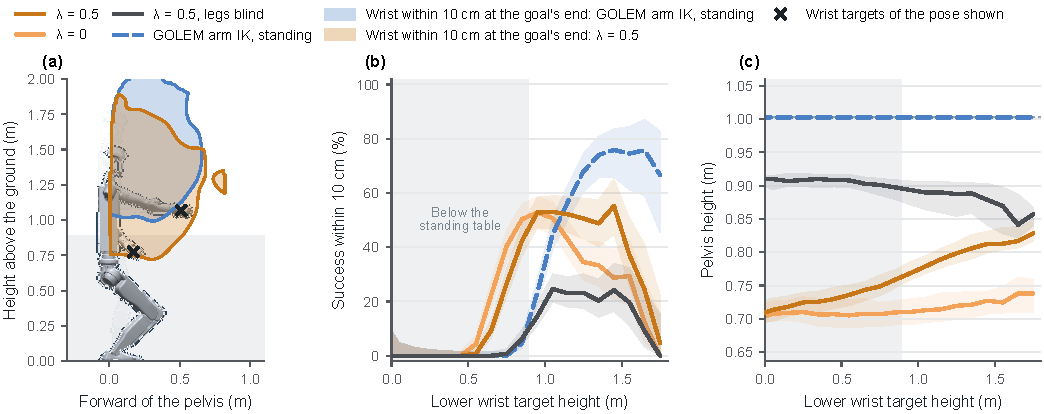
\includegraphics[width=\textwidth]{reach/figures/fig_hero.pdf}
  \caption{Reach of the $\lambda = 1$ policy with and without its legs' cooperation, on \reach{goals}{n} fixed
    goals. Left: wrist targets reached in at least half of the trials, drawn over the H1-2 in side view, for the
    policy with blind legs (blue) and the full policy (orange); the robot is shown at the end of a successful
    reach of the lowest goal it reached, with the standing pose behind it. Centre: success against the height of
    the lower wrist target. Right: pelvis height over the last second of each goal. Grey: targets below the
    lowest standing-reachable pose. Bands are 95\% Wilson intervals (centre) and interquartile ranges (right).}
  \label{fig:reach}
\end{figure*}

Of the goals whose lower target lies below the standing tables, the $\lambda = 1$ policy reached
\reach{l1/isaac}{success_below}\% and the same networks with blind legs reached
\reach{l1/isaac_legs_blind}{success_below}\%; GOLEM IK reached \reach{golem_ik/kinematic}{success_below}\% of
the \reach{golem_ik/kinematic}{n_below} such goals and \reach{golem_ik/kinematic}{success_above}\% of those above
(Fig.~\ref{fig:reach}). The operational floor was \reach{l1/isaac}{floor}\,cm above the ground for the full
policy and \reach{l1/isaac_legs_blind}{floor}\,cm with blind legs. % RESULT: one sentence on the gap.
For goals below the tables the full policy's pelvis dropped by a median of \reach{l1/isaac}{drop_below}\,cm,
against \reach{l1/isaac_legs_blind}{drop_below}\,cm with blind legs, so the crouch tracks the goal height only
when $\pi_L$ observes the goal. % RESULT: check the sign of this comparison before keeping "so".

Table~\ref{tab:depth} gives success by lowering $d$ on the unextended goals. Reaching goals 0.1 and 0.2\,m beyond
the standing tables ($e > 0$) requires leaning or stepping; the full policy reached
\reach{l1/isaac}{success_d0.0}\% of all goals at $d = 0$, which includes them.

\begin{table}[t]
  \centering
  \caption{Success (\%) by goal lowering $d$, standing-table goals without extension, three seeds per goal.}
  \label{tab:depth}
  \setlength{\tabcolsep}{4pt}
  \begin{tabular}{lrrrrrr}
    \toprule
    $d$ (m) & 0 & 0.2 & 0.4 & 0.6 & 0.8 & 1.0 \\
    \midrule
    $\lambda = 1$            & \reach{l1/isaac}{success_e0_d0.0} & \reach{l1/isaac}{success_e0_d0.2} & \reach{l1/isaac}{success_e0_d0.4} & \reach{l1/isaac}{success_e0_d0.6} & \reach{l1/isaac}{success_e0_d0.8} & \reach{l1/isaac}{success_e0_d1.0} \\
    $\lambda = 1$, blind legs & \reach{l1/isaac_legs_blind}{success_e0_d0.0} & \reach{l1/isaac_legs_blind}{success_e0_d0.2} & \reach{l1/isaac_legs_blind}{success_e0_d0.4} & \reach{l1/isaac_legs_blind}{success_e0_d0.6} & \reach{l1/isaac_legs_blind}{success_e0_d0.8} & \reach{l1/isaac_legs_blind}{success_e0_d1.0} \\
    $\lambda = 1$, IK arms   & \reach{l1/isaac_arms_ik}{success_e0_d0.0} & \reach{l1/isaac_arms_ik}{success_e0_d0.2} & \reach{l1/isaac_arms_ik}{success_e0_d0.4} & \reach{l1/isaac_arms_ik}{success_e0_d0.6} & \reach{l1/isaac_arms_ik}{success_e0_d0.8} & \reach{l1/isaac_arms_ik}{success_e0_d1.0} \\
    $\lambda = 0.5$          & \reach{l0.5/isaac}{success_e0_d0.0} & \reach{l0.5/isaac}{success_e0_d0.2} & \reach{l0.5/isaac}{success_e0_d0.4} & \reach{l0.5/isaac}{success_e0_d0.6} & \reach{l0.5/isaac}{success_e0_d0.8} & \reach{l0.5/isaac}{success_e0_d1.0} \\
    $\lambda = 0$            & \reach{l0/isaac}{success_e0_d0.0} & \reach{l0/isaac}{success_e0_d0.2} & \reach{l0/isaac}{success_e0_d0.4} & \reach{l0/isaac}{success_e0_d0.6} & \reach{l0/isaac}{success_e0_d0.8} & \reach{l0/isaac}{success_e0_d1.0} \\
    GOLEM IK (standing)      & \reach{golem_ik/kinematic}{success_e0_d0.0} & \reach{golem_ik/kinematic}{success_e0_d0.2} & \reach{golem_ik/kinematic}{success_e0_d0.4} & \reach{golem_ik/kinematic}{success_e0_d0.6} & \reach{golem_ik/kinematic}{success_e0_d0.8} & \reach{golem_ik/kinematic}{success_e0_d1.0} \\
    \bottomrule
  \end{tabular}
\end{table}

\subsection{Effect of reward sharing}
\label{sec:sharing}

Over all goals, $\lambda = 1$, $0.5$ and $0$ reached \reach{l1/isaac}{success}\%,
\reach{l0.5/isaac}{success}\% and \reach{l0/isaac}{success}\%, with operational floors of
\reach{l1/isaac}{floor}, \reach{l0.5/isaac}{floor} and \reach{l0/isaac}{floor}\,cm.
% RESULT: if lambda = 0 also crouches, the crouch follows from the legs observing the goal and sharing changes how
% far; if it does not, sharing is what produces it. State which, with the pelvis drop below the tables:
For goals below the tables their median pelvis drops were \reach{l1/isaac}{drop_below},
\reach{l0.5/isaac}{drop_below} and \reach{l0/isaac}{drop_below}\,cm.

\subsection{Balance and accuracy}
\label{sec:balance}

At $d = 0.6$\,m the $\lambda = 1$ policy kept a median minimum CoM margin of \reach{l1/isaac}{com_d0.6}\,cm and
fell in \reach{l1/isaac}{falls_d0.6}\% of trials; reached goals ended with a median wrist error of
\reach{l1/isaac}{err_d0.6}\,cm and a wrist jitter of \reach{l1/isaac}{jitter_d0.6}\,mm over the last
second, against \reach{l1/isaac}{err_d0.0}\,cm and \reach{l1/isaac}{jitter_d0.0}\,mm at $d = 0$.
Across the whole grid the policy fell in \reach{l1/isaac}{falls}\% of trials.

\subsection{Sim-to-sim transfer}
\label{sec:sim2sim}

We run the same goals in MuJoCo on the model of our lab's RoboCasa simulation, through a reimplementation of the
policy loop that reproduces the training environment's observations to $10^{-5}$ and its joint targets to
$2\times10^{-5}$\,rad from the same state, without retuning. With
RoboCasa's joint damping, armature and friction the $\lambda = 1$ policy reached \reach{l1/mujoco}{success}\%
of all goals and \reach{l1/mujoco}{success_below}\% of those below the tables, with
\reach{l1/mujoco}{falls}\% falls; with those three joint parameters set to the training values it reached
\reach{l1/mujoco_isaacphys}{success}\%. % RESULT: name the gap and its main cause.

% Sentences whose wording depends on a result still to come are marked % RESULT.
% Conditions: l1, l0.5, l0 are the three lambda runs at 91.2k steps (conditions.yaml); /isaac, /isaac_legs_blind,
% /isaac_arms_ik, /mujoco, /mujoco_isaacphys their evaluations; golem_ik/kinematic the IK reference. The preliminary
% l0.5_52k (paper_yaw_91k at 52.8k steps) is reported on the result page, not here.

\section{Experiments}
\label{sec:experiments}

We train $\pi_U$ and $\pi_L$ in Isaac Lab~\cite{mittal2025isaaclab} with the MAPPO implementation of
SKRL~\cite{serrano2023skrl}, with 4096 environments and a 50\,Hz policy over a 200\,Hz physics step, for
\wx{N environment steps} per run, one seed per $\lambda \in \{0, 0.5, 1\}$. All other settings are shared across
runs. The evaluation below holds every network and normalizer fixed and freezes the depth curriculum.

\subsection{Evaluation protocol}
\label{sec:protocol}

\textbf{Goals.} Every controller is scored on one fixed set of \reach{goals}{n} two-wrist goals. We draw
\reach{goals}{bases} pairs of wrist poses from the standing-reachable tables of Sec.~\ref{sec:upper} and lower each
pair by $d \in \{0, 0.1, \dots, \reach{goals}{depthmax}\}$\,m, the $z_{\mathrm{offset}}$ of training. To test reach away from
the body as well as below it, each lowered pair is also pushed $e \in \{0, 0.1, 0.2\}$\,m outward in the ground
plane, away from each shoulder. The lowest pose in the standing tables is \reach{goals}{standingfloor}\,cm above the
ground; a goal whose lower wrist target lies below that height cannot be reached without the legs. Goals are placed
in the standing frame at the moment they start and stay fixed in the world for 4\,s, as in training.

\textbf{Trials.} A trial resets the robot with the training reset distribution, holds a zero velocity command for
2\,s, then presents one goal. Policies act through their mean actions with observation noise on, and the learned
pelvis estimator moves the goal they observe (Sec.~\ref{sec:estimator}). We run three seeds per goal in Isaac Lab
with the training physics at its nominal values and pushes off.

\textbf{Metrics.} A trial succeeds when both wrists stay within 5\,cm and 0.35\,rad of their true world-frame goals
for 1\,s without a break, the criterion of the reach bonus. We report success with 95\% Wilson intervals, the wrist
error over the last second of successful trials, and the pelvis height over that second. For balance we report the
minimum signed distance of the centre of mass and of the divergent component of motion
$\xi = c_{xy} + \dot c_{xy}/\omega$, $\omega = \sqrt{g/z_c}$, to the edge of the support polygon, the base tilt,
planted-foot slip, and falls (tilt beyond 1\,rad). The operational floor of a controller is the lowest 0.1\,m band of
lower target height from which every band above it has at least 80\% success on the goals without extension.

\textbf{Controllers.} We compare the three $\lambda$ runs with three references. \emph{Blind legs} runs the
$\lambda = 1$ networks but gives $\pi_L$ the observation it has while standing in navigation mode, without the
wrist goals; its lower body balances and does not cooperate. \emph{IK arms} holds $\pi_U$'s residual at zero, so the
arms follow the damped-least-squares step alone. \emph{GOLEM IK} is the upper-body controller of our lab's deployed
stack, a quadratic-programming IK over the 14 arm joints with self-collision avoidance, solved on a standing robot
whose pelvis cannot move.

\subsection{Reach below the standing table}
\label{sec:reach}

\begin{figure*}[t]
  \centering
  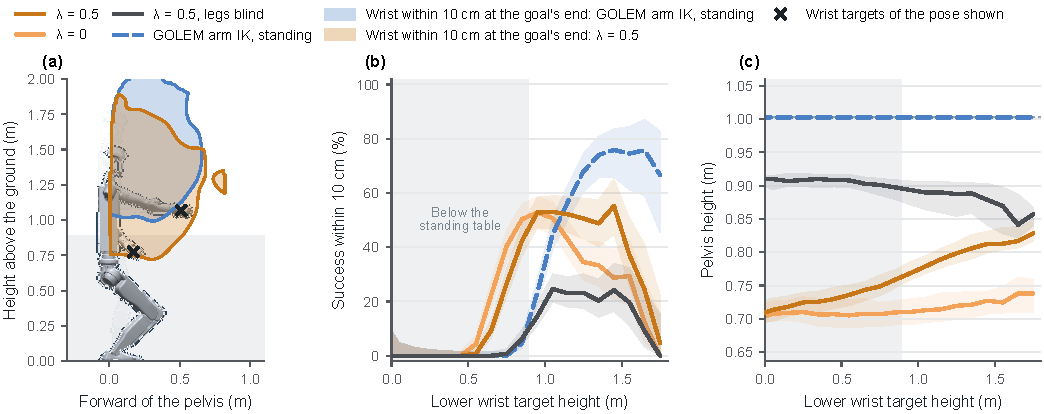
\includegraphics[width=\textwidth]{reach/figures/fig_hero.pdf}
  \caption{Reach of the $\lambda = 1$ policy with and without its legs' cooperation, on \reach{goals}{n} fixed
    goals. Left: wrist targets reached in at least half of the trials, drawn over the H1-2 in side view, for the
    policy with blind legs (blue) and the full policy (orange); the robot is shown at the end of a successful
    reach of the lowest goal it reached, with the standing pose behind it. Centre: success against the height of
    the lower wrist target. Right: pelvis height over the last second of each goal. Grey: targets below the
    lowest standing-reachable pose. Bands are 95\% Wilson intervals (centre) and interquartile ranges (right).}
  \label{fig:reach}
\end{figure*}

Of the goals whose lower target lies below the standing tables, the $\lambda = 1$ policy reached
\reach{l1/isaac}{success_below}\% and the same networks with blind legs reached
\reach{l1/isaac_legs_blind}{success_below}\%; GOLEM IK reached \reach{golem_ik/kinematic}{success_below}\% of
the \reach{golem_ik/kinematic}{n_below} such goals and \reach{golem_ik/kinematic}{success_above}\% of those above
(Fig.~\ref{fig:reach}). The operational floor was \reach{l1/isaac}{floor}\,cm above the ground for the full
policy and \reach{l1/isaac_legs_blind}{floor}\,cm with blind legs. % RESULT: one sentence on the gap.
For goals below the tables the full policy's pelvis dropped by a median of \reach{l1/isaac}{drop_below}\,cm,
against \reach{l1/isaac_legs_blind}{drop_below}\,cm with blind legs, so the crouch tracks the goal height only
when $\pi_L$ observes the goal. % RESULT: check the sign of this comparison before keeping "so".

Table~\ref{tab:depth} gives success by lowering $d$ on the unextended goals. Reaching goals 0.1 and 0.2\,m beyond
the standing tables ($e > 0$) requires leaning or stepping; the full policy reached
\reach{l1/isaac}{success_d0.0}\% of all goals at $d = 0$, which includes them.

\begin{table}[t]
  \centering
  \caption{Success (\%) by goal lowering $d$, standing-table goals without extension, three seeds per goal.}
  \label{tab:depth}
  \setlength{\tabcolsep}{4pt}
  \begin{tabular}{lrrrrrr}
    \toprule
    $d$ (m) & 0 & 0.2 & 0.4 & 0.6 & 0.8 & 1.0 \\
    \midrule
    $\lambda = 1$            & \reach{l1/isaac}{success_e0_d0.0} & \reach{l1/isaac}{success_e0_d0.2} & \reach{l1/isaac}{success_e0_d0.4} & \reach{l1/isaac}{success_e0_d0.6} & \reach{l1/isaac}{success_e0_d0.8} & \reach{l1/isaac}{success_e0_d1.0} \\
    $\lambda = 1$, blind legs & \reach{l1/isaac_legs_blind}{success_e0_d0.0} & \reach{l1/isaac_legs_blind}{success_e0_d0.2} & \reach{l1/isaac_legs_blind}{success_e0_d0.4} & \reach{l1/isaac_legs_blind}{success_e0_d0.6} & \reach{l1/isaac_legs_blind}{success_e0_d0.8} & \reach{l1/isaac_legs_blind}{success_e0_d1.0} \\
    $\lambda = 1$, IK arms   & \reach{l1/isaac_arms_ik}{success_e0_d0.0} & \reach{l1/isaac_arms_ik}{success_e0_d0.2} & \reach{l1/isaac_arms_ik}{success_e0_d0.4} & \reach{l1/isaac_arms_ik}{success_e0_d0.6} & \reach{l1/isaac_arms_ik}{success_e0_d0.8} & \reach{l1/isaac_arms_ik}{success_e0_d1.0} \\
    $\lambda = 0.5$          & \reach{l0.5/isaac}{success_e0_d0.0} & \reach{l0.5/isaac}{success_e0_d0.2} & \reach{l0.5/isaac}{success_e0_d0.4} & \reach{l0.5/isaac}{success_e0_d0.6} & \reach{l0.5/isaac}{success_e0_d0.8} & \reach{l0.5/isaac}{success_e0_d1.0} \\
    $\lambda = 0$            & \reach{l0/isaac}{success_e0_d0.0} & \reach{l0/isaac}{success_e0_d0.2} & \reach{l0/isaac}{success_e0_d0.4} & \reach{l0/isaac}{success_e0_d0.6} & \reach{l0/isaac}{success_e0_d0.8} & \reach{l0/isaac}{success_e0_d1.0} \\
    GOLEM IK (standing)      & \reach{golem_ik/kinematic}{success_e0_d0.0} & \reach{golem_ik/kinematic}{success_e0_d0.2} & \reach{golem_ik/kinematic}{success_e0_d0.4} & \reach{golem_ik/kinematic}{success_e0_d0.6} & \reach{golem_ik/kinematic}{success_e0_d0.8} & \reach{golem_ik/kinematic}{success_e0_d1.0} \\
    \bottomrule
  \end{tabular}
\end{table}

\subsection{Effect of reward sharing}
\label{sec:sharing}

Over all goals, $\lambda = 1$, $0.5$ and $0$ reached \reach{l1/isaac}{success}\%,
\reach{l0.5/isaac}{success}\% and \reach{l0/isaac}{success}\%, with operational floors of
\reach{l1/isaac}{floor}, \reach{l0.5/isaac}{floor} and \reach{l0/isaac}{floor}\,cm.
% RESULT: if lambda = 0 also crouches, the crouch follows from the legs observing the goal and sharing changes how
% far; if it does not, sharing is what produces it. State which, with the pelvis drop below the tables:
For goals below the tables their median pelvis drops were \reach{l1/isaac}{drop_below},
\reach{l0.5/isaac}{drop_below} and \reach{l0/isaac}{drop_below}\,cm.

\subsection{Balance and accuracy}
\label{sec:balance}

At $d = 0.6$\,m the $\lambda = 1$ policy kept a median minimum CoM margin of \reach{l1/isaac}{com_d0.6}\,cm and
fell in \reach{l1/isaac}{falls_d0.6}\% of trials; reached goals ended with a median wrist error of
\reach{l1/isaac}{err_d0.6}\,cm and a wrist jitter of \reach{l1/isaac}{jitter_d0.6}\,mm over the last
second, against \reach{l1/isaac}{err_d0.0}\,cm and \reach{l1/isaac}{jitter_d0.0}\,mm at $d = 0$.
Across the whole grid the policy fell in \reach{l1/isaac}{falls}\% of trials.

\subsection{Sim-to-sim transfer}
\label{sec:sim2sim}

We run the same goals in MuJoCo on the model of our lab's RoboCasa simulation, through a reimplementation of the
policy loop that reproduces the training environment's observations to $10^{-5}$ and its joint targets to
$2\times10^{-5}$\,rad from the same state, without retuning. With
RoboCasa's joint damping, armature and friction the $\lambda = 1$ policy reached \reach{l1/mujoco}{success}\%
of all goals and \reach{l1/mujoco}{success_below}\% of those below the tables, with
\reach{l1/mujoco}{falls}\% falls; with those three joint parameters set to the training values it reached
\reach{l1/mujoco_isaacphys}{success}\%. % RESULT: name the gap and its main cause.

% Sentences whose wording depends on a result still to come are marked % RESULT.
% Conditions: l1, l0.5, l0 are the three lambda runs at 91.2k steps (conditions.yaml); /isaac, /isaac_legs_blind,
% /isaac_arms_ik, /mujoco, /mujoco_isaacphys their evaluations; golem_ik/kinematic the IK reference. The preliminary
% l0.5_52k (paper_yaw_91k at 52.8k steps) is reported on the result page, not here.

\section{Experiments}
\label{sec:experiments}

We train $\pi_U$ and $\pi_L$ in Isaac Lab~\cite{mittal2025isaaclab} with the MAPPO implementation of
SKRL~\cite{serrano2023skrl}, with 4096 environments and a 50\,Hz policy over a 200\,Hz physics step, for
\wx{N environment steps} per run, one seed per $\lambda \in \{0, 0.5, 1\}$. All other settings are shared across
runs. The evaluation below holds every network and normalizer fixed and freezes the depth curriculum.

\subsection{Evaluation protocol}
\label{sec:protocol}

\textbf{Goals.} Every controller is scored on one fixed set of \reach{goals}{n} two-wrist goals. We draw
\reach{goals}{bases} pairs of wrist poses from the standing-reachable tables of Sec.~\ref{sec:upper} and lower each
pair by $d \in \{0, 0.1, \dots, \reach{goals}{depthmax}\}$\,m, the $z_{\mathrm{offset}}$ of training. To test reach away from
the body as well as below it, each lowered pair is also pushed $e \in \{0, 0.1, 0.2\}$\,m outward in the ground
plane, away from each shoulder. The lowest pose in the standing tables is \reach{goals}{standingfloor}\,cm above the
ground; a goal whose lower wrist target lies below that height cannot be reached without the legs. Goals are placed
in the standing frame at the moment they start and stay fixed in the world for 4\,s, as in training.

\textbf{Trials.} A trial resets the robot with the training reset distribution, holds a zero velocity command for
2\,s, then presents one goal. Policies act through their mean actions with observation noise on, and the learned
pelvis estimator moves the goal they observe (Sec.~\ref{sec:estimator}). We run three seeds per goal in Isaac Lab
with the training physics at its nominal values and pushes off.

\textbf{Metrics.} A trial succeeds when both wrists stay within 5\,cm and 0.35\,rad of their true world-frame goals
for 1\,s without a break, the criterion of the reach bonus. We report success with 95\% Wilson intervals, the wrist
error over the last second of successful trials, and the pelvis height over that second. For balance we report the
minimum signed distance of the centre of mass and of the divergent component of motion
$\xi = c_{xy} + \dot c_{xy}/\omega$, $\omega = \sqrt{g/z_c}$, to the edge of the support polygon, the base tilt,
planted-foot slip, and falls (tilt beyond 1\,rad). The operational floor of a controller is the lowest 0.1\,m band of
lower target height from which every band above it has at least 80\% success on the goals without extension.

\textbf{Controllers.} We compare the three $\lambda$ runs with three references. \emph{Blind legs} runs the
$\lambda = 1$ networks but gives $\pi_L$ the observation it has while standing in navigation mode, without the
wrist goals; its lower body balances and does not cooperate. \emph{IK arms} holds $\pi_U$'s residual at zero, so the
arms follow the damped-least-squares step alone. \emph{GOLEM IK} is the upper-body controller of our lab's deployed
stack, a quadratic-programming IK over the 14 arm joints with self-collision avoidance, solved on a standing robot
whose pelvis cannot move.

\subsection{Reach below the standing table}
\label{sec:reach}

\begin{figure*}[t]
  \centering
  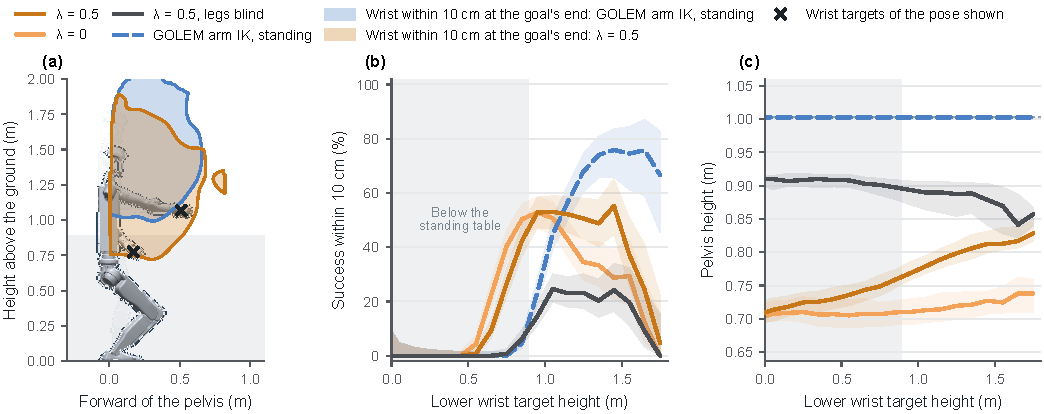
\includegraphics[width=\textwidth]{reach/figures/fig_hero.pdf}
  \caption{Reach of the $\lambda = 1$ policy with and without its legs' cooperation, on \reach{goals}{n} fixed
    goals. Left: wrist targets reached in at least half of the trials, drawn over the H1-2 in side view, for the
    policy with blind legs (blue) and the full policy (orange); the robot is shown at the end of a successful
    reach of the lowest goal it reached, with the standing pose behind it. Centre: success against the height of
    the lower wrist target. Right: pelvis height over the last second of each goal. Grey: targets below the
    lowest standing-reachable pose. Bands are 95\% Wilson intervals (centre) and interquartile ranges (right).}
  \label{fig:reach}
\end{figure*}

Of the goals whose lower target lies below the standing tables, the $\lambda = 1$ policy reached
\reach{l1/isaac}{success_below}\% and the same networks with blind legs reached
\reach{l1/isaac_legs_blind}{success_below}\%; GOLEM IK reached \reach{golem_ik/kinematic}{success_below}\% of
the \reach{golem_ik/kinematic}{n_below} such goals and \reach{golem_ik/kinematic}{success_above}\% of those above
(Fig.~\ref{fig:reach}). The operational floor was \reach{l1/isaac}{floor}\,cm above the ground for the full
policy and \reach{l1/isaac_legs_blind}{floor}\,cm with blind legs. % RESULT: one sentence on the gap.
For goals below the tables the full policy's pelvis dropped by a median of \reach{l1/isaac}{drop_below}\,cm,
against \reach{l1/isaac_legs_blind}{drop_below}\,cm with blind legs, so the crouch tracks the goal height only
when $\pi_L$ observes the goal. % RESULT: check the sign of this comparison before keeping "so".

Table~\ref{tab:depth} gives success by lowering $d$ on the unextended goals. Reaching goals 0.1 and 0.2\,m beyond
the standing tables ($e > 0$) requires leaning or stepping; the full policy reached
\reach{l1/isaac}{success_d0.0}\% of all goals at $d = 0$, which includes them.

\begin{table}[t]
  \centering
  \caption{Success (\%) by goal lowering $d$, standing-table goals without extension, three seeds per goal.}
  \label{tab:depth}
  \setlength{\tabcolsep}{4pt}
  \begin{tabular}{lrrrrrr}
    \toprule
    $d$ (m) & 0 & 0.2 & 0.4 & 0.6 & 0.8 & 1.0 \\
    \midrule
    $\lambda = 1$            & \reach{l1/isaac}{success_e0_d0.0} & \reach{l1/isaac}{success_e0_d0.2} & \reach{l1/isaac}{success_e0_d0.4} & \reach{l1/isaac}{success_e0_d0.6} & \reach{l1/isaac}{success_e0_d0.8} & \reach{l1/isaac}{success_e0_d1.0} \\
    $\lambda = 1$, blind legs & \reach{l1/isaac_legs_blind}{success_e0_d0.0} & \reach{l1/isaac_legs_blind}{success_e0_d0.2} & \reach{l1/isaac_legs_blind}{success_e0_d0.4} & \reach{l1/isaac_legs_blind}{success_e0_d0.6} & \reach{l1/isaac_legs_blind}{success_e0_d0.8} & \reach{l1/isaac_legs_blind}{success_e0_d1.0} \\
    $\lambda = 1$, IK arms   & \reach{l1/isaac_arms_ik}{success_e0_d0.0} & \reach{l1/isaac_arms_ik}{success_e0_d0.2} & \reach{l1/isaac_arms_ik}{success_e0_d0.4} & \reach{l1/isaac_arms_ik}{success_e0_d0.6} & \reach{l1/isaac_arms_ik}{success_e0_d0.8} & \reach{l1/isaac_arms_ik}{success_e0_d1.0} \\
    $\lambda = 0.5$          & \reach{l0.5/isaac}{success_e0_d0.0} & \reach{l0.5/isaac}{success_e0_d0.2} & \reach{l0.5/isaac}{success_e0_d0.4} & \reach{l0.5/isaac}{success_e0_d0.6} & \reach{l0.5/isaac}{success_e0_d0.8} & \reach{l0.5/isaac}{success_e0_d1.0} \\
    $\lambda = 0$            & \reach{l0/isaac}{success_e0_d0.0} & \reach{l0/isaac}{success_e0_d0.2} & \reach{l0/isaac}{success_e0_d0.4} & \reach{l0/isaac}{success_e0_d0.6} & \reach{l0/isaac}{success_e0_d0.8} & \reach{l0/isaac}{success_e0_d1.0} \\
    GOLEM IK (standing)      & \reach{golem_ik/kinematic}{success_e0_d0.0} & \reach{golem_ik/kinematic}{success_e0_d0.2} & \reach{golem_ik/kinematic}{success_e0_d0.4} & \reach{golem_ik/kinematic}{success_e0_d0.6} & \reach{golem_ik/kinematic}{success_e0_d0.8} & \reach{golem_ik/kinematic}{success_e0_d1.0} \\
    \bottomrule
  \end{tabular}
\end{table}

\subsection{Effect of reward sharing}
\label{sec:sharing}

Over all goals, $\lambda = 1$, $0.5$ and $0$ reached \reach{l1/isaac}{success}\%,
\reach{l0.5/isaac}{success}\% and \reach{l0/isaac}{success}\%, with operational floors of
\reach{l1/isaac}{floor}, \reach{l0.5/isaac}{floor} and \reach{l0/isaac}{floor}\,cm.
% RESULT: if lambda = 0 also crouches, the crouch follows from the legs observing the goal and sharing changes how
% far; if it does not, sharing is what produces it. State which, with the pelvis drop below the tables:
For goals below the tables their median pelvis drops were \reach{l1/isaac}{drop_below},
\reach{l0.5/isaac}{drop_below} and \reach{l0/isaac}{drop_below}\,cm.

\subsection{Balance and accuracy}
\label{sec:balance}

At $d = 0.6$\,m the $\lambda = 1$ policy kept a median minimum CoM margin of \reach{l1/isaac}{com_d0.6}\,cm and
fell in \reach{l1/isaac}{falls_d0.6}\% of trials; reached goals ended with a median wrist error of
\reach{l1/isaac}{err_d0.6}\,cm and a wrist jitter of \reach{l1/isaac}{jitter_d0.6}\,mm over the last
second, against \reach{l1/isaac}{err_d0.0}\,cm and \reach{l1/isaac}{jitter_d0.0}\,mm at $d = 0$.
Across the whole grid the policy fell in \reach{l1/isaac}{falls}\% of trials.

\subsection{Sim-to-sim transfer}
\label{sec:sim2sim}

We run the same goals in MuJoCo on the model of our lab's RoboCasa simulation, through a reimplementation of the
policy loop that reproduces the training environment's observations to $10^{-5}$ and its joint targets to
$2\times10^{-5}$\,rad from the same state, without retuning. With
RoboCasa's joint damping, armature and friction the $\lambda = 1$ policy reached \reach{l1/mujoco}{success}\%
of all goals and \reach{l1/mujoco}{success_below}\% of those below the tables, with
\reach{l1/mujoco}{falls}\% falls; with those three joint parameters set to the training values it reached
\reach{l1/mujoco_isaacphys}{success}\%. % RESULT: name the gap and its main cause.

% Sentences whose wording depends on a result still to come are marked % RESULT.
% Conditions: l1, l0.5, l0 are the three lambda runs at 91.2k steps (conditions.yaml); /isaac, /isaac_legs_blind,
% /isaac_arms_ik, /mujoco, /mujoco_isaacphys their evaluations; golem_ik/kinematic the IK reference. The preliminary
% l0.5_52k (paper_yaw_91k at 52.8k steps) is reported on the result page, not here.

\section{Experiments}
\label{sec:experiments}

We train $\pi_U$ and $\pi_L$ in Isaac Lab~\cite{mittal2025isaaclab} with the MAPPO implementation of
SKRL~\cite{serrano2023skrl}, with 4096 environments and a 50\,Hz policy over a 200\,Hz physics step, for
\wx{N environment steps} per run, one seed per $\lambda \in \{0, 0.5, 1\}$. All other settings are shared across
runs. The evaluation below holds every network and normalizer fixed and freezes the depth curriculum.

\subsection{Evaluation protocol}
\label{sec:protocol}

\textbf{Goals.} Every controller is scored on one fixed set of \reach{goals}{n} two-wrist goals. We draw
\reach{goals}{bases} pairs of wrist poses from the standing-reachable tables of Sec.~\ref{sec:upper} and lower each
pair by $d \in \{0, 0.1, \dots, \reach{goals}{depthmax}\}$\,m, the $z_{\mathrm{offset}}$ of training. To test reach away from
the body as well as below it, each lowered pair is also pushed $e \in \{0, 0.1, 0.2\}$\,m outward in the ground
plane, away from each shoulder. The lowest pose in the standing tables is \reach{goals}{standingfloor}\,cm above the
ground; a goal whose lower wrist target lies below that height cannot be reached without the legs. Goals are placed
in the standing frame at the moment they start and stay fixed in the world for 4\,s, as in training.

\textbf{Trials.} A trial resets the robot with the training reset distribution, holds a zero velocity command for
2\,s, then presents one goal. Policies act through their mean actions with observation noise on, and the learned
pelvis estimator moves the goal they observe (Sec.~\ref{sec:estimator}). We run three seeds per goal in Isaac Lab
with the training physics at its nominal values and pushes off.

\textbf{Metrics.} A trial succeeds when both wrists stay within 5\,cm and 0.35\,rad of their true world-frame goals
for 1\,s without a break, the criterion of the reach bonus. We report success with 95\% Wilson intervals, the wrist
error over the last second of successful trials, and the pelvis height over that second. For balance we report the
minimum signed distance of the centre of mass and of the divergent component of motion
$\xi = c_{xy} + \dot c_{xy}/\omega$, $\omega = \sqrt{g/z_c}$, to the edge of the support polygon, the base tilt,
planted-foot slip, and falls (tilt beyond 1\,rad). The operational floor of a controller is the lowest 0.1\,m band of
lower target height from which every band above it has at least 80\% success on the goals without extension.

\textbf{Controllers.} We compare the three $\lambda$ runs with three references. \emph{Blind legs} runs the
$\lambda = 1$ networks but gives $\pi_L$ the observation it has while standing in navigation mode, without the
wrist goals; its lower body balances and does not cooperate. \emph{IK arms} holds $\pi_U$'s residual at zero, so the
arms follow the damped-least-squares step alone. \emph{GOLEM IK} is the upper-body controller of our lab's deployed
stack, a quadratic-programming IK over the 14 arm joints with self-collision avoidance, solved on a standing robot
whose pelvis cannot move.

\subsection{Reach below the standing table}
\label{sec:reach}

\begin{figure*}[t]
  \centering
  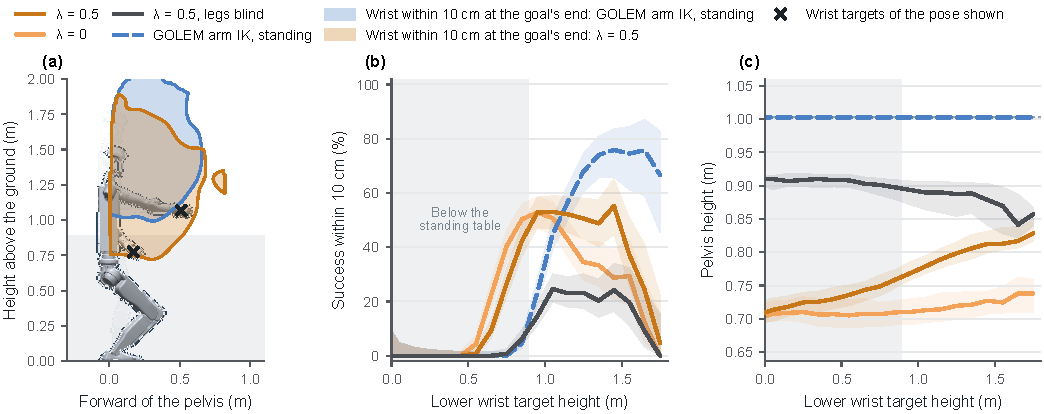
\includegraphics[width=\textwidth]{reach/figures/fig_hero.pdf}
  \caption{Reach of the $\lambda = 1$ policy with and without its legs' cooperation, on \reach{goals}{n} fixed
    goals. Left: wrist targets reached in at least half of the trials, drawn over the H1-2 in side view, for the
    policy with blind legs (blue) and the full policy (orange); the robot is shown at the end of a successful
    reach of the lowest goal it reached, with the standing pose behind it. Centre: success against the height of
    the lower wrist target. Right: pelvis height over the last second of each goal. Grey: targets below the
    lowest standing-reachable pose. Bands are 95\% Wilson intervals (centre) and interquartile ranges (right).}
  \label{fig:reach}
\end{figure*}

Of the goals whose lower target lies below the standing tables, the $\lambda = 1$ policy reached
\reach{l1/isaac}{success_below}\% and the same networks with blind legs reached
\reach{l1/isaac_legs_blind}{success_below}\%; GOLEM IK reached \reach{golem_ik/kinematic}{success_below}\% of
the \reach{golem_ik/kinematic}{n_below} such goals and \reach{golem_ik/kinematic}{success_above}\% of those above
(Fig.~\ref{fig:reach}). The operational floor was \reach{l1/isaac}{floor}\,cm above the ground for the full
policy and \reach{l1/isaac_legs_blind}{floor}\,cm with blind legs. % RESULT: one sentence on the gap.
For goals below the tables the full policy's pelvis dropped by a median of \reach{l1/isaac}{drop_below}\,cm,
against \reach{l1/isaac_legs_blind}{drop_below}\,cm with blind legs, so the crouch tracks the goal height only
when $\pi_L$ observes the goal. % RESULT: check the sign of this comparison before keeping "so".

Table~\ref{tab:depth} gives success by lowering $d$ on the unextended goals. Reaching goals 0.1 and 0.2\,m beyond
the standing tables ($e > 0$) requires leaning or stepping; the full policy reached
\reach{l1/isaac}{success_d0.0}\% of all goals at $d = 0$, which includes them.

\begin{table}[t]
  \centering
  \caption{Success (\%) by goal lowering $d$, standing-table goals without extension, three seeds per goal.}
  \label{tab:depth}
  \setlength{\tabcolsep}{4pt}
  \begin{tabular}{lrrrrrr}
    \toprule
    $d$ (m) & 0 & 0.2 & 0.4 & 0.6 & 0.8 & 1.0 \\
    \midrule
    $\lambda = 1$            & \reach{l1/isaac}{success_e0_d0.0} & \reach{l1/isaac}{success_e0_d0.2} & \reach{l1/isaac}{success_e0_d0.4} & \reach{l1/isaac}{success_e0_d0.6} & \reach{l1/isaac}{success_e0_d0.8} & \reach{l1/isaac}{success_e0_d1.0} \\
    $\lambda = 1$, blind legs & \reach{l1/isaac_legs_blind}{success_e0_d0.0} & \reach{l1/isaac_legs_blind}{success_e0_d0.2} & \reach{l1/isaac_legs_blind}{success_e0_d0.4} & \reach{l1/isaac_legs_blind}{success_e0_d0.6} & \reach{l1/isaac_legs_blind}{success_e0_d0.8} & \reach{l1/isaac_legs_blind}{success_e0_d1.0} \\
    $\lambda = 1$, IK arms   & \reach{l1/isaac_arms_ik}{success_e0_d0.0} & \reach{l1/isaac_arms_ik}{success_e0_d0.2} & \reach{l1/isaac_arms_ik}{success_e0_d0.4} & \reach{l1/isaac_arms_ik}{success_e0_d0.6} & \reach{l1/isaac_arms_ik}{success_e0_d0.8} & \reach{l1/isaac_arms_ik}{success_e0_d1.0} \\
    $\lambda = 0.5$          & \reach{l0.5/isaac}{success_e0_d0.0} & \reach{l0.5/isaac}{success_e0_d0.2} & \reach{l0.5/isaac}{success_e0_d0.4} & \reach{l0.5/isaac}{success_e0_d0.6} & \reach{l0.5/isaac}{success_e0_d0.8} & \reach{l0.5/isaac}{success_e0_d1.0} \\
    $\lambda = 0$            & \reach{l0/isaac}{success_e0_d0.0} & \reach{l0/isaac}{success_e0_d0.2} & \reach{l0/isaac}{success_e0_d0.4} & \reach{l0/isaac}{success_e0_d0.6} & \reach{l0/isaac}{success_e0_d0.8} & \reach{l0/isaac}{success_e0_d1.0} \\
    GOLEM IK (standing)      & \reach{golem_ik/kinematic}{success_e0_d0.0} & \reach{golem_ik/kinematic}{success_e0_d0.2} & \reach{golem_ik/kinematic}{success_e0_d0.4} & \reach{golem_ik/kinematic}{success_e0_d0.6} & \reach{golem_ik/kinematic}{success_e0_d0.8} & \reach{golem_ik/kinematic}{success_e0_d1.0} \\
    \bottomrule
  \end{tabular}
\end{table}

\subsection{Effect of reward sharing}
\label{sec:sharing}

Over all goals, $\lambda = 1$, $0.5$ and $0$ reached \reach{l1/isaac}{success}\%,
\reach{l0.5/isaac}{success}\% and \reach{l0/isaac}{success}\%, with operational floors of
\reach{l1/isaac}{floor}, \reach{l0.5/isaac}{floor} and \reach{l0/isaac}{floor}\,cm.
% RESULT: if lambda = 0 also crouches, the crouch follows from the legs observing the goal and sharing changes how
% far; if it does not, sharing is what produces it. State which, with the pelvis drop below the tables:
For goals below the tables their median pelvis drops were \reach{l1/isaac}{drop_below},
\reach{l0.5/isaac}{drop_below} and \reach{l0/isaac}{drop_below}\,cm.

\subsection{Balance and accuracy}
\label{sec:balance}

At $d = 0.6$\,m the $\lambda = 1$ policy kept a median minimum CoM margin of \reach{l1/isaac}{com_d0.6}\,cm and
fell in \reach{l1/isaac}{falls_d0.6}\% of trials; reached goals ended with a median wrist error of
\reach{l1/isaac}{err_d0.6}\,cm and a wrist jitter of \reach{l1/isaac}{jitter_d0.6}\,mm over the last
second, against \reach{l1/isaac}{err_d0.0}\,cm and \reach{l1/isaac}{jitter_d0.0}\,mm at $d = 0$.
Across the whole grid the policy fell in \reach{l1/isaac}{falls}\% of trials.

\subsection{Sim-to-sim transfer}
\label{sec:sim2sim}

We run the same goals in MuJoCo on the model of our lab's RoboCasa simulation, through a reimplementation of the
policy loop that reproduces the training environment's observations to $10^{-5}$ and its joint targets to
$2\times10^{-5}$\,rad from the same state, without retuning. With
RoboCasa's joint damping, armature and friction the $\lambda = 1$ policy reached \reach{l1/mujoco}{success}\%
of all goals and \reach{l1/mujoco}{success_below}\% of those below the tables, with
\reach{l1/mujoco}{falls}\% falls; with those three joint parameters set to the training values it reached
\reach{l1/mujoco_isaacphys}{success}\%. % RESULT: name the gap and its main cause.
